%%%%%%%%%%%%%%%%%%%%%%%%%%%%%%%%%%%%%%%%%%%%%%%%%%%%
% Document type, global settings, and packages
%%%%%%%%%%%%%%%%%%%%%%%%%%%%%%%%%%%%%%%%%%%%%%%%%%%%

\documentclass[12pt]{report}   %12 point font for Times New Roman
\usepackage{graphicx}  %for images and plots
\usepackage[letterpaper, left=1.5in, right=1in, top=1in, bottom=1in]{geometry}
\usepackage{setspace}  %use this package to set linespacing as desired
\usepackage{times}  %set Times New Roman as the font
\usepackage[explicit]{titlesec}  %title control and formatting
\usepackage[titles]{tocloft}  %table of contents control and formatting
\usepackage[backend=bibtex, style=numeric-comp,sortcites=true,sorting=none, bibstyle=nature]{biblatex}  %reference manager
\usepackage[bookmarks=true, hidelinks]{hyperref}
	%\renewcommand{\chapterautorefname}{Chapter} %Make chapter-->Chapter

\usepackage{booktabs} %for tables lines
\usepackage[page]{appendix}  %for appendices
\usepackage{rotating}  %for rotated, landscape images
\usepackage[normalem]{ulem}  %for italicized text
\usepackage{epigraph}
\usepackage{amsmath, amsthm, amssymb, amsfonts} %Math libraries
\renewcommand{\vec}[1]{\mathbf{#1}} %Vector bold
\DeclareMathOperator{\erf}{erf}    %erf


\usepackage[font=small,labelfont=bf]{caption} %Caption control
\usepackage{siunitx}       %SI Units
\usepackage[symbols,nogroupskip,nonumberlist,stylemods,style=index]{glossaries-extra} %Glossary
\usepackage{indentfirst} %Indents first para after chapter and section
\usepackage[hang, flushmargin, bottom]{footmisc} %Footnote at bottom only
%Footnote with no marker
\newcommand\blfootnote[1]{%
  \begingroup
  \renewcommand\thefootnote{}\footnote{#1}%
  \addtocounter{footnote}{-1}%
  \endgroup
}
\usepackage[nameinlink]{cleveref} %CleverCrossRef
\crefname{appendix}{Appendix}{Appendices} %Creating appendix reference


\usepackage[textcolor=black,figwidth=0.5\linewidth,disable]{todonotes} 
%%%%%%%%%%%%%%%%%%%%%%%%%%%%%%%%%%%
% Notes
%%%%%%%%%%%%%%%%%%%%%%%%%%%%%%%%%%%
  %Notes for writing to disable \usepackage[disable]{todonotes}
\reversemarginpar
\makeatletter
\renewcommand{\todo}[2][]{%
    \@todo[caption={#2}, #1]{\begin{spacing}{0.5}#2\end{spacing}}%
} 
\makeatother 

%%%%%%%%%%%%%%%%%%%%%%%%%%%%%%%%%%%
% Glossary
%%%%%%%%%%%%%%%%%%%%%%%%%%%%%%%%%%%
%\setlength{\glsdescwidth}{15cm}
%\newglossary[slg]{symbolslist}{syi}{syg}{Symbolslist} % create add. symbolslist
%\glsaddkey{unit}{\glsentrytext{\glslabel}}{\glsentryunit}{\GLsentryunit}{\glsunit}{\Glsunit}{\GLSunit}
%\glssetnoexpandfield{unit}
\makeglossaries                                   % activate glossaries-package
\loadglsentries{glossary}
%%%%%%%%%%%%%%%%%%%%%%%%%%%%%%%%%%%
% Bibliography
%%%%%%%%%%%%%%%%%%%%%%%%%%%%%%%%%%%

%Add your bibliography file here
\bibliography{references/HeatLibrary-newUU.bib}

%Add your graphics path here
\graphicspath{{figures/}}

% prevent certain fields in references from printing in bibliography
\AtEveryBibitem{\clearfield{issn}}
\AtEveryBibitem{\clearlist{issn}}

\AtEveryBibitem{\clearfield{language}}
\AtEveryBibitem{\clearlist{language}}

\AtEveryBibitem{\clearfield{doi}}
\AtEveryBibitem{\clearlist{doi}}

\AtEveryBibitem{\clearfield{url}}
\AtEveryBibitem{\clearlist{url}}

\AtEveryBibitem{\clearfield{issue}}
\AtEveryBibitem{\clearlist{issue}}

\AtEveryBibitem{\clearfield{month}}
\AtEveryBibitem{\clearlist{month}}

\AtEveryBibitem{%
	\ifentrytype{online}
	{}
	{\clearfield{urlyear}\clearfield{urlmonth}\clearfield{urlday}}}
	
%%%%%%%%%%%%%%%%%%%%%%
%%%%%%My Commands%%%%%%%%%
\newcommand{\angstrom}{\textup{\AA}}
\newcommand{\sige}[2]{Si$_{#1}$Ge$_{#2}$}
\newcommand{\algas}[2]{Al$_{#1}$Ga$_{#2}$As}
%\newcommand{\nm}{nm}
\newcommand{\etal}{\textit{et al.}\ }

%%%%%%%%%%%%%%%%%%%%%%
% Start of Document
%%%%%%%%%%%%%%%%%%%%%%

\begin{document}
\doublespacing  %set line spacing

%%%%%%%%%%%%%%%%%%%%%%%%%%%%%%%%%%%%%
% Title Page
%%%%%%%%%%%%%%%%%%%%%%%%%%%%%%%%%%%%%

%% Define your thesis title, your name, your school, and your month and year of graduation here

\newcommand{\thesisTitle}{Exploring Thermal Transport in Semiconductor Nanostructures}
\newcommand{\yourName}{Abhinav Malhotra}
\newcommand{\yourSchool}{Chemical \& Biomolecular Engineering}
\newcommand{\yourMonth}{August}
\newcommand{\yourYear}{2019}

%%%%%%%%%%%%%%%%%%%%%%%%%%%%%%%%%%%%%%%%%%%%%%%%%%%%%%%%%
% Do not edit these lines unless you wish to customize
% the template
%%%%%%%%%%%%%%%%%%%%%%%%%%%%%%%%%%%%%%%%%%%%%%%%%%%%%%%%%



\begin{titlepage}
\begin{center}

\begin{singlespacing}

\textbf{\MakeUppercase{\thesisTitle}}\\
\vspace{10\baselineskip}
A Dissertation\\
Presented to\\
The Academic Faculty\\
\vspace{3\baselineskip}
By\\
\vspace{3\baselineskip}
\yourName\\
\vspace{3\baselineskip}
In Partial Fulfillment\\
of the Requirements for the Degree\\
Doctor of Philosophy in the\\
School of \yourSchool\\
\vspace{3\baselineskip}
Georgia Institute of Technology\\
\vspace{\baselineskip}
\yourMonth{} \yourYear{}
\vfill
Copyright \copyright{} \yourName{} \yourYear{}

\end{singlespacing}

\end{center}
\end{titlepage}



\currentpdfbookmark{Title Page}{titlePage}  %add PDF bookmark for this page

%%%%%%%%%%%%%%%%%%%%%%%%%%%%%%%%%%%%%
% Approval Page
%%%%%%%%%%%%%%%%%%%%%%%%%%%%%%%%%%%%%

%% Define your committee members. If you have less than 6, simple delete/comment the unused lines

\newcommand{\committeeMemberOne}{Dr. Martin Maldovan, Advisor}
\newcommand{\committeeMemberOneDepartment}{School of Chemical \& Biomolecular Engineering \newline School of Physics}
\newcommand{\committeeMemberOneAffiliation}{Georgia Institute of Technology}

\newcommand{\committeeMemberTwo}{Dr. David S. Sholl}
\newcommand{\committeeMemberTwoDepartment}{School of Chemical \& Biomolecular Engineering}
\newcommand{\committeeMemberTwoAffiliation}{Georgia Institute of Technology}

\newcommand{\committeeMemberThree}{Dr. Elsa Reichmanis}
\newcommand{\committeeMemberThreeDepartment}{School of Chemical \& Biomolecular Engineering}
\newcommand{\committeeMemberThreeAffiliation}{Georgia Institute of Technology}

\newcommand{\committeeMemberFour}{Dr. Michael A. Filler}
\newcommand{\committeeMemberFourDepartment}{School of Chemical \& Biomolecular Engineering}
\newcommand{\committeeMemberFourAffiliation}{Georgia Institute of Technology}

\newcommand{\committeeMemberFive}{Dr. Zhuomin Zhang}
\newcommand{\committeeMemberFiveDepartment}{George W. Woodruff School of Mechanical Engineering}
\newcommand{\committeeMemberFiveAffiliation}{Georgia Institute of Technology}

\newcommand{\approvalDay}{08}
\newcommand{\approvalMonth}{July}
\newcommand{\approvalYear}{2019}

%%%%%%%%%%%%%%%%%%%%%%%%%%%%%%%%%%%%%%%%%%%%%%%%%%%%%%%%%
% Do not edit these lines unless you wish to customize
% the template
%%%%%%%%%%%%%%%%%%%%%%%%%%%%%%%%%%%%%%%%%%%%%%%%%%%%%%%%%


\begin{titlepage}
\begin{singlespacing}
\begin{center}

\textbf{\MakeUppercase{\thesisTitle}}\\
\vspace{10\baselineskip}

\end{center}
\vfill

%Define minipages, depending on how many authors there are
\ifdefined\committeeMemberFour

Approved by:
\vspace{2\baselineskip}		%adjust the number in front of "\baselineskip" for alignment

\begin{minipage}[b]{0.41\textwidth}
	
	\committeeMemberOne\\
	\committeeMemberOneDepartment\\
	\textit{\committeeMemberOneAffiliation}\\
	
	\committeeMemberTwo\\
	\committeeMemberTwoDepartment\\
	\textit{\committeeMemberTwoAffiliation}\\
	
	\committeeMemberThree\\
	\committeeMemberThreeDepartment\\
	\textit{\committeeMemberThreeAffiliation}\\
	
	\vspace{0\baselineskip}		%adjust the number in front of "\baselineskip" for alignment
	
\end{minipage}
\hspace{0.1\textwidth}
\begin{minipage}[b]{0.41\textwidth}
	
	\committeeMemberFour\\
	\committeeMemberFourDepartment\\
	\textit{\committeeMemberFourAffiliation}\\
	\vskip 1\baselineskip       %I added
	
	\ifdefined\committeeMemberSix
	\committeeMemberFive\\
	\committeeMemberFiveDepartment\\
	\textit{\committeeMemberFiveAffiliation}\\
	
	\committeeMemberSix\\
	\committeeMemberSixDepartment\\
	\textit{\committeeMemberSixAffiliation}\\
	%REDUNDDANT
	\vspace{-4\baselineskip}    
	Date Approved: \approvalMonth{} \approvalDay, \approvalYear
	\vspace{3\baselineskip}		%adjust the number in front of "\baselineskip" for alignment
	
	\else
	%-------MY OPERATION HERE
	\committeeMemberFive\\
	\committeeMemberFiveDepartment\\
	\textit{\committeeMemberFiveAffiliation}\\
	\vskip -1\baselineskip
	\leavevmode
	\\ \\ \\ \\ \\ \\ Date Approved: \approvalMonth{} \approvalDay, \approvalYear
	\vspace{-1.2\baselineskip}		%adjust the number in front of "\baselineskip" for alignment
	
	\fi
	
\end{minipage}

\else

\hspace{0.6\textwidth}
\begin{minipage}[b]{0.4\textwidth}
	
	Approved by:
	\vspace{2\baselineskip}		%adjust the number in front of "\baselineskip" for alignment
	
	\committeeMemberOne\\
	\committeeMemberOneDepartment\\
	\textit{\committeeMemberOneAffiliation}\\
	
	\committeeMemberTwo\\
	\committeeMemberTwoDepartment\\
	\textit{\committeeMemberTwoAffiliation}\\
	
	\committeeMemberThree\\
	\committeeMemberThreeDepartment\\
	\textit{\committeeMemberThreeAffiliation}\\
	
	\vspace{2\baselineskip}		%adjust the number in front of "\baselineskip" for alignment
	
	Date Approved: \approvalMonth{} \approvalDay, \approvalYear
	\vspace{\baselineskip}		%adjust the number in front of "\baselineskip" for alignment
	
\end{minipage}

\fi





\end{singlespacing}
\end{titlepage}


%%%%%%%%%%%%%%%%%%%%%%%%%%%%%%%%%%%%%
% Epigraph
%%%%%%%%%%%%%%%%%%%%%%%%%%%%%%%%%%%%%

%% Define your quote and author for the epigraph here

\newcommand{\yourQuote}{Their minds sang with the ecstatic knowledge that either what they were doing was completely and utterly and totally impossible or that physics had a lot of catching up to do. \newline}
\newcommand{\yourAuthor}{The Hitchhiker's Guide to Galaxy}

%%%%%%%%%%%%%%%%%%%%%%%%%%%%%%%%%%%%%%%%%%%%%%%%%%%%%%%%%
% Do not edit these lines unless you wish to customize
% the template
%%%%%%%%%%%%%%%%%%%%%%%%%%%%%%%%%%%%%%%%%%%%%%%%%%%%%%%%%

\begin{titlepage}
\begin{center}

\vspace*{\fill}
\yourQuote\\ 
\textit{\yourAuthor}
\vspace*{\fill}

\end{center}
\end{titlepage}



%%%%%%%%%%%%%%%%%%%%%%%%%%%%%%%%%%%%%
% Dedication
%%%%%%%%%%%%%%%%%%%%%%%%%%%%%%%%%%%%%

% Define your dedication statement here

\newcommand{\yourDedication}{To Mom and Dad.}

%%%%%%%%%%%%%%%%%%%%%%%%%%%%%%%%%%%%%%%%%%%%%%%%%%%%%%%%%
% Do not edit these lines unless you wish to customize
% the template
%%%%%%%%%%%%%%%%%%%%%%%%%%%%%%%%%%%%%%%%%%%%%%%%%%%%%%%%%

\begin{titlepage}
\begin{center}

\vspace*{\fill}
\yourDedication\\
\vspace*{\fill}

\end{center}
\end{titlepage}


%%%%%%%%%%%%%%%%%%%%%%%%%%%%%%%%%%%%%
% Acknowledgments
%%%%%%%%%%%%%%%%%%%%%%%%%%%%%%%%%%%%%

\pagenumbering{roman}
\addcontentsline{toc}{chapter}{Acknowledgments}
\setcounter{page}{4} % set the page number appropriately based on the number of intro pages
\setlength{\parskip}{1em}
\clearpage
\begin{centering}
\textbf{ACKNOWLEDGEMENTS}\\
\vspace{\baselineskip}
\end{centering}

%Insert your dedication text here
Last five years have presented me with amazing opportunities and I have a lot of people to thank for this extraordinary journey. Foremost, my advisor Dr. Martin Maldovan whose passion for science and patience for naive questions made him the perfect mentor for me. I am forever grateful to him for exposing me to a wide-array of ideas; we had some amazing discussions on topics from technology to philosophy, filled with stimulating thoughts and boisterous laughter, which I will always cherish.

I am particularly grateful to Dr. Michael Filler for his feedback on my research and it has been a pleasure to learn from his insights. His podcast, Nanovation, continues to fuel my interest in nanotechnology while making commutes more bearable. I am also grateful to Dr. Zhuomin Zhang, Dr. David Sholl and Dr. Elsa Reichmanis for letting me learn from their vast academic experience and always providing me helpful feedback about my research. 

I would like to acknowledge my experimental collaborators, Dr. Gözde Tütüncüoglu, Dr. Shannon Yee and his research lab, Dr. Sampath Kommandur, Aravindh Rajan and Patrick Creamer. I also thank my group and office-mates Dr. Juan Manuel and Kartik Kothari for amazing discussions we had and ideas that we produced these past years. Georgia Tech has really been a cracking place to work because of all of you! 

I am grateful to the Defense Advanced Research Projects Agency (DARPA), Defense Sciences Office (DSO), and the Army Research Office (ARO) for their financial support of my PhD.

I would like to recognize my mentors at IIT Roorkee, Dr. Shashi and Dr. Surendra Kumar who instilled in me a passion for research. Dr. Shashi was an inspiration for me and will always be dearly missed.

My biggest supporters, my Mom and Dad, thank you for all the things that you have done for me and selflessly supporting me in all my decisions. My brother Dr. Suhail Malhotra for being the best partner in crime. We have always made each other a little better and a little stronger, one day at a time. I am also ever grateful to my sister-in-law Dr. Parminder for her infectious optimism in everything that she does, to Rishi Sidhu for the numerous discussions we continue to share that always make my days brighter, to my uncle Dr. Satpal Ahuja who continues to be a role model to pursue excellence, quietly and honestly, and to all my friends I made in Atlanta, in particular Mayank, Kong and Anshuman, for being a part of special moments that shaped my last five years. 

Finally, the one person who has accompanied me on nearly every step of this journey, Akanksha. She has been my best friend a long time before I decided to come to Georgia Tech. From the decision to come to Atlanta together, to listening to multiple iterations of almost every presentation, she has selflessly been there every step of the way. It was her positive outlook and unending support that propelled me onwards. Thank you for giving meaning to everything that I do.

\clearpage
%\pagenumbering{gobble}  %remove page number on summary page

\setlength{\parskip}{0em}
%\addtocontents{toc}{\cftpagenumbersoff{chapter}}

%\currentpdfbookmark{Acknowledgments}{acknowledgments}
%\addtocontents{toc}{\cftpagenumberson{chapter}}


%%%%%%%%%%%%%%%%%%%%%%%%%%%%%%%%%%%%%
% Table of Contents
%%%%%%%%%%%%%%%%%%%%%%%%%%%%%%%%%%%%%

% Format for Table of Contents
\renewcommand{\cftchapdotsep}{\cftdotsep}  %add dot separators
\renewcommand{\cftchapfont}{\bfseries}  %set title font weight
\renewcommand{\cftchappagefont}{}  %set page number font weight
\renewcommand{\cftchappresnum}{Chapter }
\renewcommand{\cftchapaftersnum}{:}
\renewcommand{\cftchapnumwidth}{5em}
\renewcommand{\cftchapafterpnum}{\vskip\baselineskip} %set correct spacing for entries in single space environment
\renewcommand{\cftsecafterpnum}{\vskip\baselineskip}  %set correct spacing for entries in single space environment
\renewcommand{\cftsubsecafterpnum}{\vskip\baselineskip} %set correct spacing for entries in single space environment
\renewcommand{\cftsubsubsecafterpnum}{\vskip\baselineskip} %set correct spacing for entries in single space environment

%format title font size and position (this also applys to list of figures and list of tables)
\titleformat{\chapter}[display]
{\normalfont\bfseries\filcenter}{\chaptertitlename\ \thechapter}{0pt}{\MakeUppercase{#1}}

\renewcommand\contentsname{Table of Contents}

\begin{singlespace}
\tableofcontents
\end{singlespace}

\currentpdfbookmark{Table of Contents}{TOC}

\clearpage

%%%%%%%%%%%%%%%%%%%%%%%%%%%%%%%%%%%%%
% List of figures and tables
%%%%%%%%%%%%%%%%%%%%%%%%%%%%%%%%%%%%%

\addcontentsline{toc}{chapter}{List of Tables}
\begin{singlespace}
	\setlength\cftbeforetabskip{\baselineskip}  %manually set spacing between entries
	\listoftables
\end{singlespace}

\clearpage

\addcontentsline{toc}{chapter}{List of Figures}
\begin{singlespace}
\setlength\cftbeforefigskip{\baselineskip}  %manually set spacing between entries
\listoffigures
\end{singlespace}

\clearpage

%%%%%%%%%%%%%%%%%%%%%%%%%%%%%%%%%%%%%
%List of abbreviations
%%%%%%%%%%%%%%%%%%%%%%%%%%%%%%%%%%%%%
%\addcontentsline{toc}{chapter}{List of Symbols}
%\begin{singlespace}
\printunsrtglossary[type=symbols, style=long3col, title={List of Symbols}]
%\end{singlespace}



%%%%%%%%%%%%%%%%%%%%%%%%%%%%%%%%%%%%%%%%%%%%%%%%%%%%%%%%%%%%%%%%%
% This is the Summary (abstract should be separate document)
%%%%%%%%%%%%%%%%%%%%%%%%%%%%%%%%%%%%%%%%%%%%%%%%%%%%%%%%%%%%%%%%%
\setlength{\parskip}{1.0em}
\clearpage
\thispagestyle{empty}
\begin{centering}
\textbf{SUMMARY}\\
\vspace{\baselineskip}
\end{centering}

Advances in nanotechnology have opened doors for a rational design of semiconductor materials with engineered thermal properties. This ability to control nanoscale thermal transport properties is key for advancing multiple technologies including thermoelectrics which have immense potential as power generators as well as for waste-heat recovery, optoelectronics such as quantum cascade lasers which are used in applications from long-range communication to medical surgery, and the ubiquitous microelectronic transistors which power our laptops and phones. Thus, a fundamental understanding of the conduction of heat in semiconductor nanostructures is foundational for accelerating human progress.

The conduction of heat in solid state semiconductors is controlled by the thermal vibrations that originate on the application of a thermal gradient. These thermal vibrations, or phonons, are the carriers of heat whose transport properties can be controlled via their interactions with surfaces in the nanostructure. Thus, the flow of heat can be modulated by designing the nanostructure and engineering the phonon-surface interaction. Predicting the flow of heat at nanometer length scales by modeling the interaction of phonons with surfaces in a nanostructure in order to understand thermal conduction in semiconductor nanostructures is the central objective of this thesis. 

To achieve this objective, we first create a predictive model for nanoscale thermal transport for nanowires and thin-films in \Cref{chap:predictive}. The created model incorporates experimentally quantifiable descriptors, such as surface roughness and correlation length, in order to evaluate the role of phonon reflection from surfaces on thermal transport. We extend the predictive model in \Cref{chap:diff_boundary} to a  generic case where both the surfaces of the thin-film are distinct, a situation that arises in experimental growth of free-standing thin-films, and show the  spatial evolution of thermal flux in thin-films as a function of surface conditions analogous to fluid flow in confined geometries. We use the case of distinct boundaries to model nanotubes in \Cref{chap:nt}, which have recently gained experimental attention. Importantly, in all of these cases we can predict not only the thermal conductivity but also the proportion of heat carried by individual phonons which is key for rational thermal material design.

In the second half of the thesis we focus on planar layered nanostructures to understand the effects of phonon transmission (in addition to reflection) on thermal properties. In \Cref{chap:layered} we model planar bi-layer and tri-layer nanostructures and show that contrary to the commonly held notion that thermal conductivity at the nanoscale can only be reduced, these layered structures present an opportunity to locally enhance thermal conductivity. We uncover the phenomenon of phonon injection that is central to these effects. We also apply the newly developed understanding to film-on-substrate systems, which are a common semiconductor growth platform and highlight the importance of phonon coupling effects on thermal properties of this system. In \Cref{chap:slxp}, we study cross-plane thermal transport in superlattices and predict the role of all relevant length scales, i.e. surface roughness, period length and superlattice size on thermal properties, which would be of profound practical importance.

Overall, we have created thermal transport models for a variety of nanostructures which include cylindrical cross-section structures -- nanowires and nanotubes, and planar structures -- thin-films, bi-layers, tri-layers and superlattices. We elucidated the role of phonon scattering at surfaces (both reflection and transmission) in experimentally realizable nanostructures using quantifiable surface descriptors. The methodology and the findings of this thesis advance nanoscale thermal transport literature by providing a fundamental and quantitative understanding about the transport of heat in semiconductor nanostructures.


%\todo{revisit.}
\pagenumbering{gobble}  %remove page number on summary page

%%%%%%%%%%%%%%%%%%%%%%%%%%%%
%
% Chapters
%
%%%%%%%%%%%%%%%%%%%%%%%%%%%%
\setlength\epigraphwidth{8cm}
\setlength\epigraphrule{0pt}

%%%%%%%%%%%%%%%%%%%%%%
% formatting
%%%%%%%%%%%%%%%%%%%%%%

% resume page numbering for rest of document
\clearpage
\pagenumbering{arabic}
\setcounter{page}{1} % set the page number appropriately

% Adjust chapter title formatting
\titleformat{\chapter}[display]
{\normalfont\bfseries\filcenter}{\MakeUppercase\chaptertitlename\ \thechapter}{0pt}{\MakeUppercase{#1}}  %spacing between titles
\titlespacing*{\chapter}
  {0pt}{0pt}{30pt}	%controls vertical margins on title

% Adjust section title formatting
\titleformat{\section}{\normalfont\bfseries}{\thesection}{1em}{#1}

% Adjust subsection title formatting
\titleformat{\subsection}{\normalfont}{\uline{\thesubsection}}{0em}{\uline{\hspace{1em}#1}}

% Adjust subsubsection title formatting
\titleformat{\subsubsection}{\normalfont\itshape}{\thesubsection}{1em}{#1}

%%%%%%%%%%%%%%%%
% Chapter 1
%%%%%%%%%%%%%%%%
\setlength{\parskip}{0em}
%!TEX root = thesis.tex
\chapter{Introduction}
\label{chap:intro}

\section{Heat and Nanotechnology}

The understanding and control of thermal transport processes has been central to human progress over the course of our evolution. From the discovery of fire by friction, to harnessing the thermal energy via the steam engine, the path of human progress has been paved with thermal energy. Now, with the burgeoning advances in nanotechnology, understanding and controlling heat flow at the nanoscale has become a key scientific and technological challenge. Just as the in-depth understanding of transport of electrons and photons revolutionized the fields of electronics and photonics \cite{RN486,book_maldovan}, similar degree of progress in nanoscale phononics (phonon is the thermal carrier in semiconductor solids) has the potential to propel energy research and create fundamental and novel discoveries about flow of heat. Technologically, nanoscale thermal conduction is central to the performance of microelectronic processors, optoelectronic devices such as lasers and light emitting diodes, and for energy materials such as thermoelectrics. Take for instance the modern-day nanometer scale computer processors, these high performance devices can have localized spatial locations called hot-spots where the magnitude of thermal flux \gls{J} can exceed 10 \si{\watt\per\centi\meter\squared} \cite{rev_Majum_thermoelec,rev_Moore} a value greater than the Solar flux reaching the Earth (Solar constant = 0.13 \si{\watt\per\centi\meter\squared}) \cite{solarconstant}. The efficient dissipation of heat is central to the usability of these devices. In addition to the lack of space to incorporate heat dissipation solutions, the problem is further compounded by the reduction of thermal conductivity at these nano length scales as compared to the bulk \cite{book_Zhuomin}. This reduction of thermal conduction arises from the interaction of heat carriers (i.e. phonons) with nanostructures, which inhibits their heat transporting ability. Furthermore, heat dissipation also impacts the efficiency of optoelectronic devices such as photo-detectors and light emitting diodes \cite{book_rogalski_infrared}. The reduced nanoscale thermal conductivities are not always negative in their impact, as low thermal conductivity coupled with high electrical conductivity allows thermoelectric devices to convert waste-heat into electricity efficiently. These thermoelectrics further have the capability to generate power for off-grid applications and to even cool down microelectronic hot-spots \cite{rev_snyder,rev_thermoelec_tritt,rev_Majum_thermoelec}. Due to its ubiquity, thermal energy transport thus remains central to current technological development and these examples are illustrative of the potential impact that a rational thermal design of nanoscale materials can have in advancing important technologies central to the modern civilization.

  \section{Nanoscale Thermal Conduction and Phonons}
Thermal conduction is the dominant mechanism of heat conduction in solids, and occurs when a temperature gradient, which acts as the thermal driving force, is applied across the solid. Fourier's Law is used in bulk systems to describe the heat conduction \cite{book_Bird},

\begin{equation}
J_x = -\kappa \nabla_x T
\label{eq:fourier}
\end{equation} 

where \gls{Jx} is the the conductive thermal flux generated by the applied temperature gradient \gls{gradT} in the $x$-direction, and \gls{K} is the corresponding thermal conductivity in the same direction.  The microscopic origins of thermal conduction lie in the vibrations of atoms that create a net transport of energy from the hotter end to the cooler end \cite{book_Reif}. From this atomic perspective, thermal transport in non-metallic crystalline solids is described as the transport of atomic vibrations with broadband frequencies that are generated and move under an applied temperature gradient. Quantized lattice vibrations are called \textit{phonons} and can be considered to be the particles of heat \cite{book_Ashcroft}. Thermal conduction in semiconductor nanostructures can thus be described as the net transport of phonons from the high temperature region to the low temperature region. 
\par Phonons are characterized by their frequency \gls{freq} of vibration, their propagation wavevector \gls{k}, and their longitudinal or transversal polarization. Phonons in solid materials can exist in a broadband range of frequencies \gls{freq} determined by the dispersion relation $\omega(\mathbf{k})$, a fundamental material property giving the relation between the phonon frequency  \gls{freq} and the phonon wavevector \gls{k} for each polarization. Being able to establish how much heat can be conducted in a solid material requires knowledge of three fundamental phonon transport properties -- how much energy phonons can carry (\gls{hbar}\gls{freq}$_\mathbf{k}$), how fast they can move (group velocity \gls{vg}$_\mathbf{k}$), and how far they can travel (mean-free-path \gls{mfp}$_\mathbf{k}$). We note that in nanostructures, length scales smaller than mean-free-paths of bulk phonons create interactions between phonons and surfaces, which are central to the modification of thermal properties at the nanoscale. We further note that all the phonon transport properties are dependent on wavevector \gls{k} and when combined together determine ability of the material to conduct heat. Thus, the transport of heat under a thermal gradient is an aggregate behavior of phonons generated within the nanostructure at each spatial location $r$, moving along all directions with their wavevector dependent thermal transport properties, \gls{hbar}\gls{freq}$_\mathbf{k}$, \gls{vg}$_\mathbf{k}$, and \gls{mfp}$_\mathbf{k}$, and their statistically averaged transport is contained in the thermal conductivity \gls{K},

\begin{equation}
{J_x}=-\kappa \nabla_x T = -\frac{1}{t}\,{\int_{0}^{t} \sum_{pol} \Big[ \frac{1}{8 \pi^3}\iiint \hbar\omega_{\mathbf{k}}\dfrac{\partial f^{BE}}{\partial T}v^x_{\mathbf{k}}\ell^x_{\mathbf{k}}({r}) \,d^3{k} \Big]} \,d{r}\:\nabla_x T
\label{eq:phonon_fourier}
\end{equation} 

where, the contribution of each phonon at each spatial location $r$ is integrated over the complete \gls{k}-space, summed for each phonon polarization $pol$, and averaged over the size \gls{t} of the nanostructure to determine the effective thermal conductivity \gls{K} of the nanostructure in the direction of the gradient.\footnote{For calculations of thermal transport along a particular direction, say $x$, the components of group velocity \gls{vg}$^x_\mathbf{k}$ and mean-free-path \gls{mfp}$^x_\mathbf{k}$ are used.} Note that the equilibrium Bose-Einstein population \gls{fBE} is a function of temperature and phonon energy. Importantly, \Cref{eq:phonon_fourier} highlights a key fundamental physical aspect, that is nanoscale thermal conduction is a spatially local phenomenon. Under such spatial locality, phonons at different spatial location in general, have distinct mean-free-paths, and therefore contribute distinctly to thermal transport \cite{maldovan2011tf,ownSpatialTF}. This physical nature arises due to the differing influence of surfaces on different spatial  locations, and distinguishes nanoscale thermal transport from bulk-scale transport. This distinction also underlies the observation that thermal conductivity at the nanoscale is a strong function of nanostructure size \cite{book_Ziman,ownNW,ownTF}. The structure-size dependent thermal conductivity is characteristic of the \emph{quasi-ballistic transport} regime, which is the primary focus of this thesis. Contrarily, in the \emph{diffusive transport} regime, the thermal conductivity is not linked to structure size as seen at the bulk-scale \cite{book_Bird}.
 
\section{The Phonon Boltzmann Transport Equation}
A quasi-ballistic regime of phonon transport is characterized by the existence of two kinds of phonon scattering events. The first is the scattering of phonons due to nanostructure surfaces \cite{book_Ziman}. This phonon-surface interaction is spatially discrete in nature, since it can occur only at specific locations in the nanostructure, i.e. at boundaries. The second kind of interaction that occurs throughout the volume of the nanostructure is the anharmonic phonon-phonon scattering \cite{book_Ashcroft}. Other volumetric events include phonon-alloy and phonon-impurity scattering. Both kinds of scattering events -- discrete and volumetric -- influence the thermal transport in nanostructures by modifying the transport of phonons.  Thus, in order to model thermal transport for a wide range of conditions, the modeling tool of choice should at minimum possess the capability to include the scattering physics, with the flexibility of adding new features as required.

To this end, the Boltzmann transport equation (BTE) provides a rigorous framework to mathematically represent the transport of phonons. At steady state and under a single-mode relaxation time approximation, the BTE for phonons can be written as \cite{book_Ziman,ownCoupling1},

\begin{equation}
\mathbf{v}(\mathbf{k}) \cdot \nabla f(\mathbf{k},\mathbf{r})  + \frac{f(\mathbf{k},\mathbf{r})-f^{BE}(\mathbf{k},\mathbf{r})}{\tau(\mathbf{k})}=0
\label{eq:bte_ss}
\end{equation} 				
where \gls{f} is the phonon population function deviated from the equilibrium Bose-Einstein population \gls{fBE} due to the applied driving force. The relaxation time \gls{tau} accounts for the anharmonic phonon scattering effects, and can be obtained from first-principle calculations \cite{stokes_bulkSi_tau,bAs_broido}, or iteratively by matching experimental bulk conductivity measurements to model predictions \cite{aksamijaNW,maldovan2011tf}.\footnote{While both these approaches have been shown to yield similar outputs for Silicon (see \Cref{app:si_relaxation_rates}) first principle approach can be useful for new materials or materials without sufficient experiments, while the iterative approach is useful to  obtain temperature dependent functional forms of relaxation time cheaply.} For emphasis, the dependence of quantities on wavevector \gls{k} and position $r$ are explicitly written. A closed form solution to \Cref{eq:bte_ss} is nanostructure dependent and spatial boundary conditions for phononic populations are required \cite{ownKK1,ownCoupling1,ownCoupling2,RN396} . Therefore, we discuss the exact methodology for obtaining non-equilibrium phononic populations \gls{f} in specific chapters as required. Once the non-equilibrium populations are calculated as a function of position for each phonon mode, thermal conductivity can be obtained using,

\begin{equation}
J_x=-\kappa \nabla_x T = -\frac{1}{t}\,{\int_{0}^{t} \sum_{pol} \Big[ \frac{1}{8 \pi^3}\iiint \hbar\omega_{\mathbf{k}}v^x_{\mathbf{k}}f_{\mathbf{k}}({r}) \,d^3{k} \Big]} \,d{r}
\label{eq:pop_fourier}
\end{equation} 

	A comparison between \Cref{eq:phonon_fourier} and \eqref{eq:pop_fourier} shows that there is a fundamental connection between mean-free-path \gls{mfp} and phononic population \gls{f}. We explicitly show in thin-films (see \Cref{chap:diff_boundary}) that both equations are equivalent and either of them can be used to obtain thermal properties. Thus, for nanowires and nanotubes (see \Cref{chap:predictive,chap:nt}), \Cref{eq:phonon_fourier} is evaluated since geometrically obtaining mean-free-paths is simpler. On the other hand, in layered nanostructures (see \Cref{chap:layered,chap:slxp}) the calculation of phononic population \gls{f} by solving the BTE allows for a more tractable solution allowing us to evaluate \Cref{eq:pop_fourier} to obtain thermal properties in these nanostructures.
	
\section{Outline of the Thesis}
The overarching vision of this thesis is to explore the phenomenon of nanoscale thermal conduction in different nanostructures. Aligned with this vision, the work contained in this dissertation is divided into two main parts,
\begin{itemize}
\item First, we explore nanostructures in which the interaction of phonons with surfaces is focused on reflection i.e. backward scattering.  The nanostructures of this category included in this thesis are nanowires, thin-films and nanotubes. 
	\begin{itemize}
	
	\item In \Cref{chap:predictive}, we formulate a predictive mathematical model that incorporates experimentally quantifiable surface descriptors as inputs for phonon-surface scattering. Such a model allows for quantifying the role of surfaces in nanoscale thermal transport while allowing for a comparison with measurements.
	
	\item In \Cref{chap:diff_boundary}, we extend the model to a general case of thin-films with distinct surfaces. We use the model to show the spatial distribution of thermal flux and draw the analogy with fluid flow.
	
	\item In \Cref{chap:nt}, we utilize the developed model to evaluate thermal conduction in semiconductor nanotubes. This study allows for an understanding of cylindrical geometries with distinct inner and outer surfaces and is utilized in explaining experimental measurements.
	\end{itemize}
	
	\item Second, we explore nanostructures in which phonons upon interacting with surfaces can be reflected and transmitted, i.e. both backward and forward scattered. The nanostructures of this category included in this thesis are semiconductor bi-layers, tri-layers and superlattices.
	\begin{itemize}
	\item In \Cref{chap:layered}, we model layered nanostructures under an in-plane temperature gradient to understand the role of phonon transmission. This novel study allows us to uncover a novel phenomenon of phonon coupling, which can be utilized to locally modulate thermal properties at the nanoscale.
	\item In \Cref{chap:slxp}, we model cross-plane thermal transport in superlattices allowing for an exploration across multiple length scales -- roughness, period and size. 
	\end{itemize}
	
\end{itemize}







%%%%%%%%%%%%%%%%
% Chapter 2
%%%%%%%%%%%%%%%%

%!TEX root = thesis.tex
\chapter{Thermal Transport in Nanowires and Thin-Films}\label{chap:predictive}
\section{Introduction}\blfootnote{Portions of this chapter have originally been published in \cite{ownNW} ``Impact of Phonon Surface Scattering on Thermal Energy Distribution of Si and SiGe Nanowires" (2016), \textit{Scientific Reports}, Vol. 6 (25818), and in \cite{ownTF} ``Surface Scattering Controlled Heat Conduction in Semiconductor Thin Films" (2016), \textit{Journal of Applied Physics}, Vol. 120 (204305). Reproduced from \cite{ownNW} under a CC BY 4.0 License, and from \cite{ownTF} with permission from AIP Publishing.}
The development of rigorous nanoscale thermal transport models requires the inclusion of the phonon-boundary scattering effects.  At the small length scales of nanostructures such as thin-films and nanowires, the physical boundaries of these structures provide a scattering mechanism for phonons. In fact, phonon surface scattering has been extensively used in the last decade to obtain significant reductions in heat conduction, and a large number of low-thermal conductivity nanostructures have been fabricated experimentally including thin-films  \cite{RN136,RN122,RN127,RN189,RN109} and nanowires \cite{RN20,RN88,NW_hochbaum,RN111,RN130,RN337,RN483}. Despite the key role played by phonon-surface interactions, these have been treated approximately in existing models. For instance, simplified kinetic theory models have relied on the Matthiessen’s rule \cite{book_Ziman} to provide an effective relaxation time to account for the reduced mean-free-paths of phonons due to boundary scattering. The intrinsic inaccuracy in the Matthiessen’s rule is the treatment of boundary scattering as an internal volumetric phenomenon (i.e., similar to phonon-phonon scattering mechanisms), while in reality the surface interaction occurs only at discrete points located at the surface. Furthermore, theoretical models have not focused on studying the phonon-surface interaction to mathematically elucidate the underlying physics rigorously. Simplified approaches have been utilized historically which do not account for all physical variables critically needed to describe this interaction, namely -- incident phonon momentum and angle as well as the surface characteristics, such as roughness and correlation length. Commonly, these approaches include the constant specularity assumption (which ignores the momentum dependence of scattering) and Ziman’s formula (which assumes all phonons to be normally incident) \cite{book_Ziman}. In addition, contrary to established approaches in optics and acoustics \cite{RN8}, the effects of rough surface shadowing on phonon surface scattering have also been unexplored in thermal phonon transport.  As a result, there is currently a need for accurately describing phonon-surface interactions in order to understand, predict, and control heat conduction processes at the nanoscale. Without achieving such fundamental understanding, it is difficult to create truly predictive models that can transition from matching with experimentally measured thermal conductivity values towards predicting transport quantities such as thermal spectra and guiding experiments to obtain rationally designed nanostructures for thermal applications.

\section{Calculating Mean-Free-Paths in Nanowires and Thin-Films}\label{sec:MFPRedModel}
The first step in obtaining predictive models is to distinguish between discrete boundary scattering events and volumetric internal scattering events. Here, we show an approach based on the a kinetic picture of phonon transport, that allows for treating boundary scattering events as discrete \cite{maldovan2011tf,RN115}. Once the accurate phononic mean-free-paths are available, they can be used to calculate transport properties, for instance thermal conductivity as shown in \Cref{eq:phonon_fourier}. In order to do so, a fundamental statistical definition of mean-free-path is used to account for the role of boundaries on phonon transport. The probability density function for phonon internal scattering in bulk as phonons propagate internally along the path length $\xi$ given by \cite{RN221},
\begin{equation}
\dfrac{dP}{d\xi}= \dfrac{1}{\ell^{\text{bulk}}}\exp(-\dfrac{\xi}{\ell^{\text{bulk}}})
\label{eq:ch2-prob}
\end{equation}
marks the starting point of this calculation. Under the assumption that the phonons in nanostructures follow similar internal relaxation rates, the change in phononic mean-free-paths \gls{mfp} in the semiconductor nanostructures stems from the introduction of boundary scattering processes. Thus, the central aim of this section is to define a framework in which the effects of boundaries can be included to evaluate phononic mean-free-paths. For illustration, we choose a thin-film to describe the mathematics behind such a calculation, while noting that the formulation holds true for any nanostructure (including nanowires) in which the geometrical distance between two successive phonon scatterings is constant. 
% Schematic 0
\begin{figure}[hbt]
	\centering 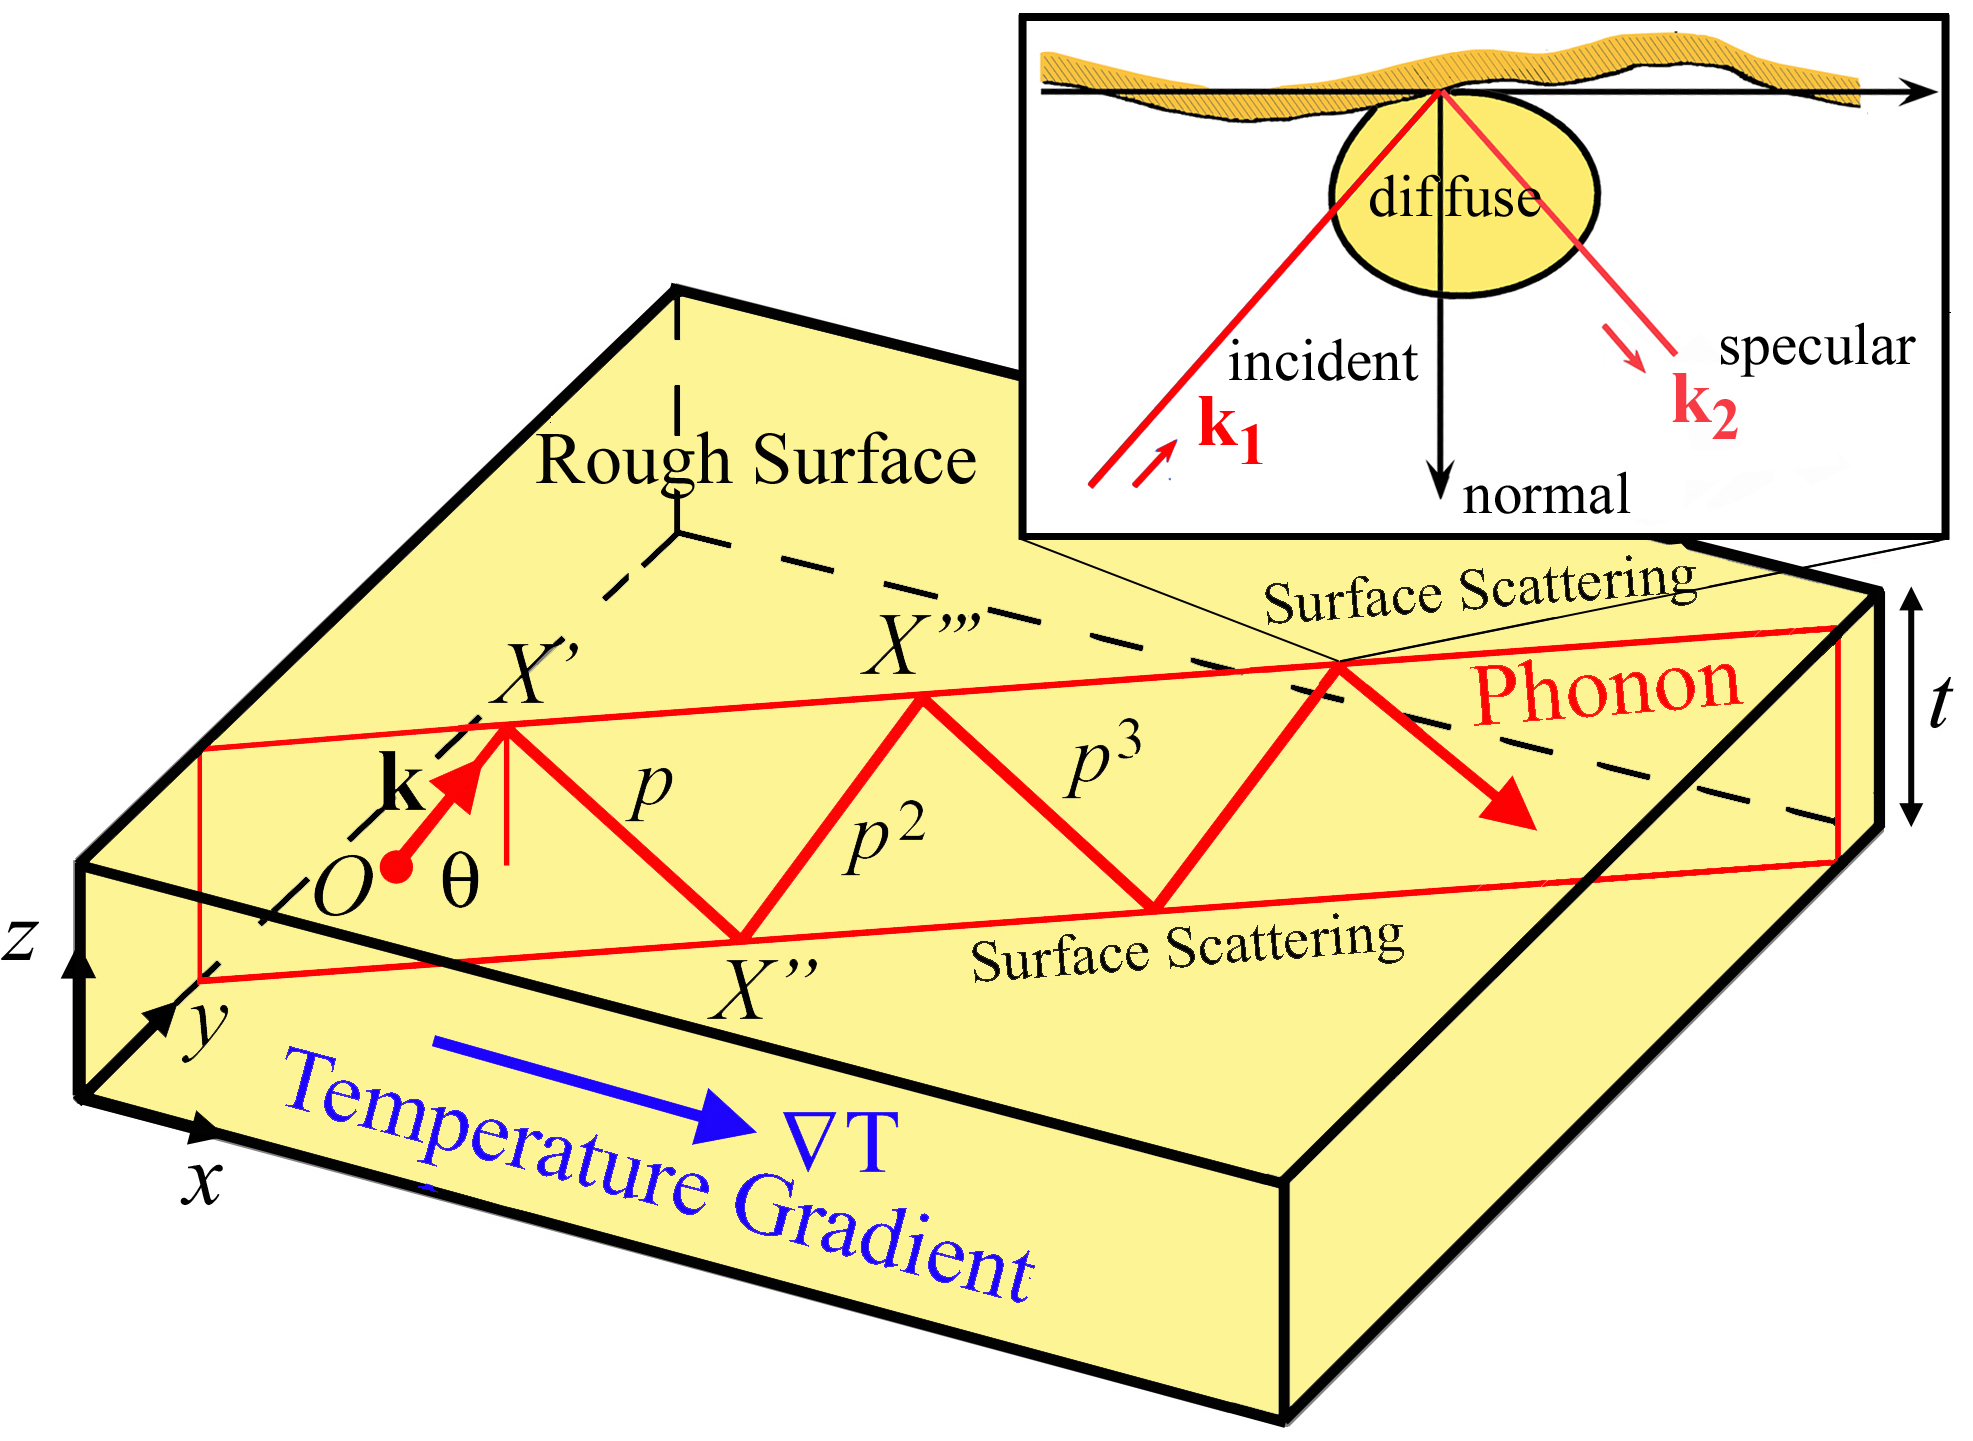
\includegraphics[width=0.95\textwidth]{/ch2/Fig1-SchematicTF.jpg}
	\caption{Schematic showing the in-plane phonon transport in a thin-film of thickness \gls{t}. The temperature gradient is applied along the $x$-direction. Phonons with wavevector \gls{k} originate at a random location O and reach the boundary at an angle \gls{theta} with the surface normal. A fraction \gls{p} of phonons are reflected specularly while the rest $1-p$ scatter diffusively at every interaction with the boundary, leading to a reduction in their mean-free-paths $\ell_{\vec{k}}$ in the thin film as compared to the bulk value $\ell^{\text{bulk}}_{\vec{k}}$.}
	\label{fig:ch2-tf_scatter_schematic}
\end{figure}
\par 
For now we lump the effect of surfaces into a \textit{specularity parameter} \gls{p} that defines the fraction of incident phonons to undergo a specular reflection, and reserve the discussion on the physical nature of the specularity parameter for \Cref{sec:BK}. During a specular reflection, a fraction \gls{p} of phonons preserve their angle of incidence \cite{book_Ziman}. On the other hand, remaining $1-p$  fraction of phonons are diffusively scattered in all directions. The diffusive scattering of a portion of phonons is central to the reduction of phononic mean-free-paths in nanostructures. For the case shown in \Cref{fig:ch2-tf_scatter_schematic}, phonons originating at point $O$ located at a distance $z$ from the upper boundary propagate at an arbitrary angle \gls{theta} with the surface normal towards the upper surface. At every interaction with the surfaces of the nanostructure, a proportion \gls{p} of incident phonons are scattered specularly, while the rest are scattered diffusively. We note that in general, phonons can encounter the interfaces repeatedly, so that in order to define their mean-free-path we use,
\begin{equation}
\ell=\int_{0}^{\infty}\xi dP
\end{equation}
By writing $OX^{'}=\Lambda$, the contribution to the mean-free-path for phonons starting at $O$ up to the point $X^{'}$ can be written as,
\begin{equation}
\ell^{{OX^{'}}}=\int_{0}^{\Lambda}{\xi dP} + (1-p)\int_{\Lambda}^{\infty}{\xi dP}
\end{equation}
where the second term represents the diffusively scattered phonons at $X^{'}$. Subsequent propagation of specularly scattered phonons from $X^{'}$ to $X^{''}$ yields the contribution,
\begin{equation}
\ell^{{X^{'}X^{''}}}=p \Bigg( \int_{\Lambda}^{\Lambda+\Lambda^*}{\xi dP} + (1-p)\int_{\Lambda+\Lambda^*}^{\infty}{\xi dP} \Bigg)
\end{equation}
where $X^{'}X^{''}=\Lambda^*=X^{'''}=...$ , allowing us to write subsequent contributions as series. We note that the mean-free-paths are dependent on phonon wave-vectors, thus we introduce a subscript \gls{k} to explicitly indicate the dependence. By using \Cref{eq:ch2-prob} to replace $dP$ with path-length traveled and sum over the total path to obtain the mean-free-paths of phonons in thin-films and nanowires as a reduction from bulk mean-free-paths.
\begin{equation}
\ell_{\vec{k}}(z)= \ell_{\vec{k}}^{\text{bulk}} \Bigg[ 1 - \dfrac{(1-p)\exp\Big(-\dfrac{\Lambda(z,\theta)}{\ell_{\vec{k}}^{\text{bulk}}}\Big)}{1-p\exp\Big(-\dfrac{\Lambda^*(t,\theta)}{\ell_{\vec{k}}^{\text{bulk}}}\Big)} \Bigg]
\label{eq:ch2-mfp_reduced}
\end{equation}

%-----------------BK--------------------
\section{Determining Specularity Parameter: Role of Surface and Phonon Properties}\label{sec:BK}
In the phonon-surface scattering process, the properties of both the surface and the incident phonons determine the dynamics. In order to characterize surfaces, a measure of the variation from a mean plane (i.e. roughness \gls{eta}) and the distance between two roughness features (i.e. correlation length 
\gls{cl}), are used. Such a description is suitable from a practical experimental standpoint as well since a surface can only be described statistically as a point-to-point description would be nearly impossible. The incident phonon properties include the incident phonon momentum ($\hbar\vec{k}$) and the incident angle with the surface normal \gls{thetai}. When a phononic population moving under an applied gradient interacts with a surface, a portion of it can be backward scattered, i.e. reflected into the same medium, while the other can be forward scattered, i.e. transmitted, across the surface into adjoining medium. These forward and backward scattering of phonons at the surface can be specular or diffuse, whose probability depends on surface properties as well as incident phonon properties. Since our purpose is to determine the specularity parameter \gls{p} for reflection, we treat the surface as a sold-air interface. To obtain the specularity parameter, the phonon field scattered by a random rough surface and its mean power over different directions is analyzed. Such a statistical behavior of rough surfaces and knowledge of their reflection coefficients have been extensively considered in studies of electromagnetic wave phenomena and acoustics \cite{RN101,book_Beckmann}. Here, we utilize the quasi-classical Beckmann-Kirchhoff (BK) framework to obtain a relation between specularity parameter and phonon wavelength, incident angle, surface roughness, and correlation length. 
\subsection{Beckmann-Kirchhoff Surface Scattering Theory}
To utilize the BK framework, we first define a one-dimensional surface S of length 2D in the ${\hat{x}}_0$ direction that separates the two solid media. Any point on such a surface can be described using a position vector \textbf{r}, 
\begin{equation}\label{eq:ch2-1} 
\mathbf{r}=x{\ \hat{\mathbf{x}}}_0+\zeta\left(x\right){\hat{\mathbf{z}}}_0                                         
\end{equation}
% Schematic 2
\begin{figure}[hbt]
	\centering 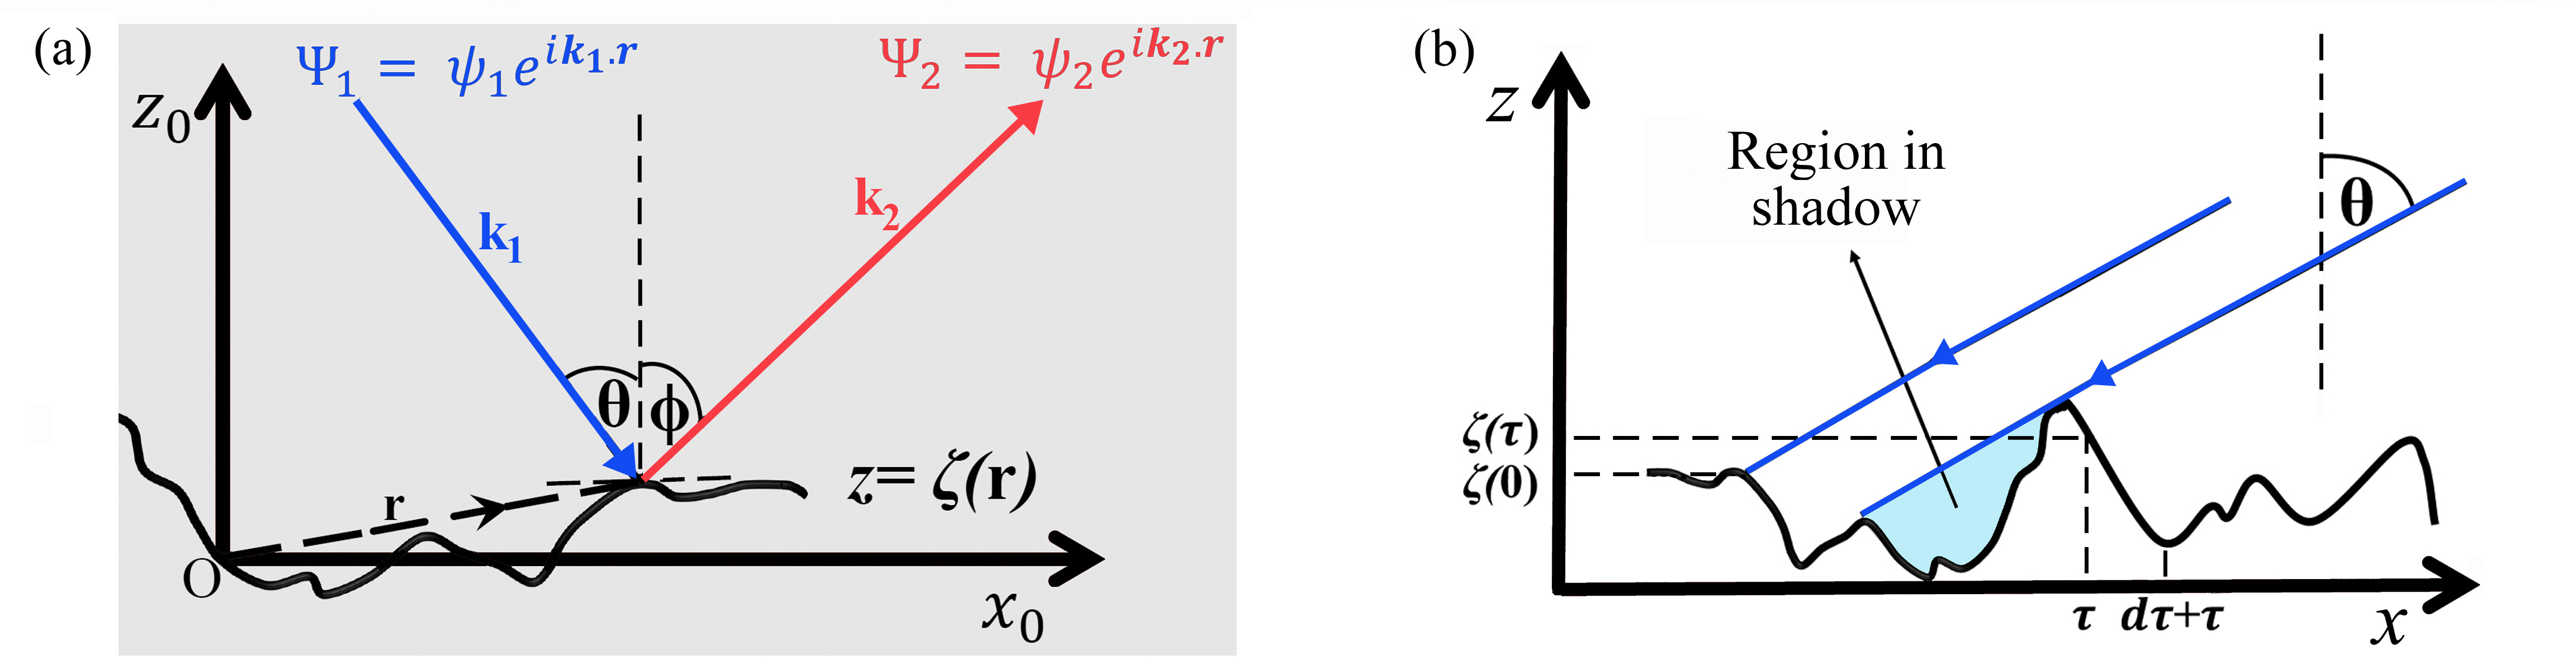
\includegraphics[width=\textwidth]{/ch2/Figure1-2.jpg}
	\caption{Schematic representation of phonon-surface interaction. (a) Incident $\Psi_{1}$ and scattered $\Psi_{2}$ phonon fields with angle of incidence \gls{theta} and scattered angle \gls{phi} from a rough surface $z = \zeta (\vec{r})$, where \gls{r} is the position vector and $\vec{k}_{1}$ and $\vec{k}_{2}$ are the corresponding wavevectors. (b) Surface shadowing. Phonons are incident with wavevector \gls{k} at angle of incidence \gls{theta} measured clockwise from the $z$ axis. Shadows are cast along the $-x$ direction reducing the surface area available for scattering.}
	\label{fig:ch2-bk_schematic2}
\end{figure}

We note that the BK method relies on the Kirchhoff approximation which requires that the surface gradients are small enough so that the field at a local tangent plane to any point on the surface approximates the field on the surface itself. Importantly, this approximation does not impose any restriction on the surface roughness (which has been a criticism of perturbation based approaches \cite{RN83}) but requires that the surface gradients are small enough so that only a minimal number of sharp features exist \cite{book_Beckmann}. Furthermore, a single scattering event from surface roughness is assumed and edge-effects are neglected. Initially, we assume that surface shadowing effects [\Cref{fig:ch2-bk_schematic2}(b)] are negligible. This is later relaxed to incorporate the effect of correlation length on specularity. In order to completely define surface properties, we assume that the distribution of surface features that obey Gaussian statistics. Under such distribution of height variations $w(z)$ around a mean plane centered at $\zeta=0$, the mathematical definition of the surface roughness can be extracted from,
\begin{equation}\label{eq:ch2-2}
w\left(z\right)=\frac{1}{\eta\sqrt(2\pi)}\exp\left(-\frac{z^2}{2\eta^2}\right)	
\end{equation}
In addition to surface roughness, a complete description of the surface also requires the information on the correlation length \gls{cl}, i.e. the distance between similar height variations. For a Gaussian distribution, the auto-correlation function enables a mathematical definition of correlation length between two repeated height variations at $x_1$ and $x_2$, and a large correlation length \gls{cl} translates to gradual slopes for the height variations. 
\begin{equation}\label{eq:ch2-31}
C\left(x_1,x_2\right)=\exp\left(-\frac{({x_1-x_2)}^2}{\mathcal{L}^2}\right)                                                  
\end{equation}
For simplification, phonons are treated as a plane-wave in this formulation with their incident field written as $\Psi_1=\psi_1e^{i\mathbf{k}_1.\mathbf{r}}$. Note that the time-dependent factor $\exp(-i\omega t)$ has been dropped since conservation of phonon energy in scattering processes is implied. Writing the Helmholtz wave equation for the total field $\Psi$,
\begin{equation}\label{eq:ch2-3}
{(\nabla}^2+k^2)\Psi=0
\end{equation}
where $k$ denotes the modulus of the wavevector \gls{k}, Green’s function theory gives the solution of the wave equation at an interior point in terms of the values of the function $\Psi$ and its normal derivative on the surface S. The scattered field $\Psi_2$ at a point of observation $X$ located at a distance $d$ from the point of incidence $(x,\zeta\left(x\right))$ at the surface is obtained using the boundary conditions, 
\begin{equation}\label{eq:ch2-4}
\Psi_{S}=(1+R)\Psi_1
\end{equation}
\begin{equation}\label{eq:ch2-5}
\left(\frac{\partial\Psi}{\partial n}\right)_{S}=\left(1-R\right)\Psi_1{\ i\ \mathbf{k}}_1.\mathbf{n}
\end{equation}
where $R$ denotes the reflection coefficient for a smooth plane and \textbf{n} is the normal to the surface. In general, $R$ may depend on the angle of incidence of the field and the physical properties of the media at both sides of the surface. However, we consider a perfectly free surface (due to the large mechanical contrast for solid-air interfaces) and therefore the reflection coefficient $R=-1$. Under the above formulation, the normalized scattered field from a one-dimensional surface yields the following expression \cite{book_Beckmann},
\begin{equation}\label{eq:ch2-6}
\widetilde{\Psi}(\theta,\varphi)=\frac{\Psi_2(\theta,\varphi)}{\Psi_2(\theta,\varphi=\theta)}=\frac{1}{2D}\sec{\theta}\frac{1+\cos{(\theta+\varphi)}}{\cos{\theta}+\cos{\varphi}}\int_{-D}^{+D}e^{i\left(\mathbf{k}_1-\mathbf{k}_2\right).\mathbf{r}}dx
\end{equation}
 where the phonons incident at angle $\theta$ and scattered at an angle $\varphi$, denoted by $\Psi_2(\theta,\varphi)$, are expressed in terms of the phonons scattered in the specular direction by a smooth, perfectly free surface with the same dimensions, i.e. $\Psi_2(\theta,\varphi=\theta)$. Using \Cref{eq:ch2-6}, we can evaluate the mean energy carried by the backward scattered phonons from the whole surface by evaluating the square of the scattered field $<\widetilde{\Psi}{\widetilde{\Psi}}^\ast>$. For the Gaussian surface under consideration here, the energy associated with the scattered field evaluates to \cite{ownNW},
\begin{equation}\label{eq:ch2-7}
\begin{split}
<\widetilde{\Psi}{\widetilde{\Psi}}^\ast>\ =\ e^{-\eta^2\left(\mathrm{k}_{1,z}-\mathrm{k}_{2,z}\right)^2}
\Bigg(\left(\frac{\sin{\left(\mathrm{k}_{1,x}D-\mathrm{k}_{2,x} D\right)}}{\left(\mathrm{k}_{1,x}D-\mathrm{k}_{2,x} D\right)}\right)^2 + \frac{\sqrt\pi\mathcal{L}}{2D}\left(\frac{1+\cos{\left(\theta+\varphi\right)}}{\cos{\theta}+\cos{\varphi}}\right)^2 \times \\ \sum_{j=1}^{\infty}\frac{\eta^{2j}\left(\mathrm{k}_{1,z}-\mathrm{k}_{2,z}\right)^{2j}}{j!\sqrt j}e^\frac{\left(\mathrm{k}_{1,x}D-\mathrm{k}_{2,x} D\right)^2\mathcal{L}^2}{4j} \Bigg)
\end{split}
\end{equation} 
%-------------------------------
% Schematic 1000000000000000000000000000
\begin{figure}[hbt]
	\centering 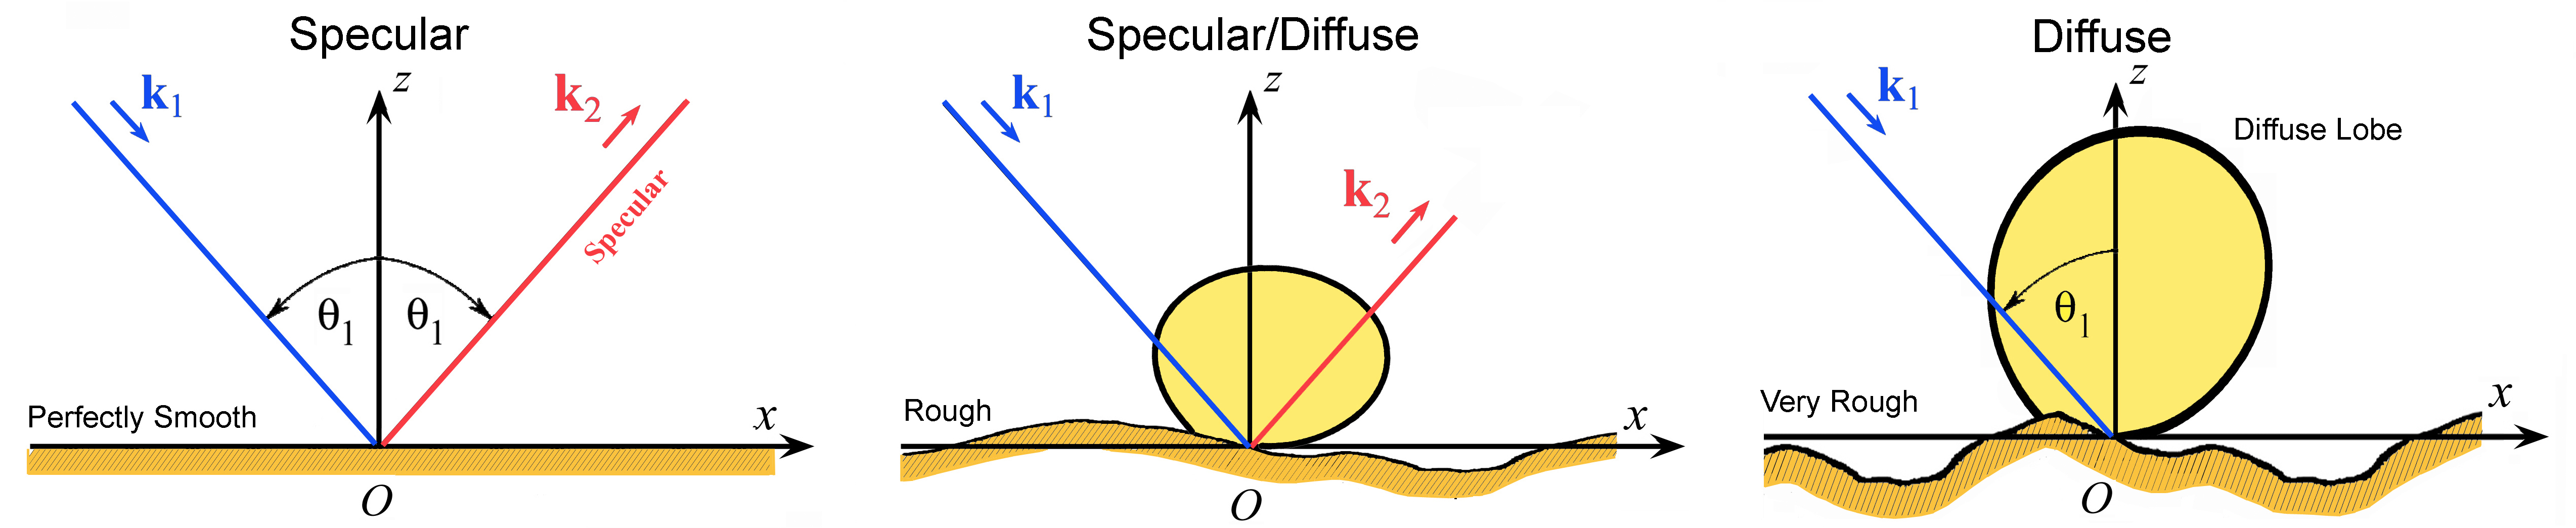
\includegraphics[width=\textwidth]{/ch2/Figure1-1.jpg}
	\caption{Schematic representation of role of roughness showing the transition from specular reflection to diffuse
scattering. \textit{Left:} Perfectly smooth surface showing perfect reflection. \textit{Centre:} Rough surface with partially
specular/partially diffuse scattering. \textit{Right:} Very rough surface exhibiting complete diffuse scattering.}
	\label{fig:ch2-bk_schematic1}
\end{figure}
%------------------
\Cref{eq:ch2-7} is also referred to as the Beckmann-Kirchhoff surface scattering model and represents a complex angular distribution of the scattered energy in a thin-film when phonons are incident at an angle $\theta$. In particular, the first term represents the specular scattering of phonons and has a sharp contribution when the scattering angle $\varphi\approx \theta$ and quickly decays at other angles. Thus, to obtain a specularity parameter \gls{p} (i.e. the proportion of specularly scattered phonons) in the limit when surface correlation length \gls{cl} is large as compared to incident phonon wavelength (i.e. $k_1\mathcal{L}\gg1$), the contribution of the first term representing the specularly scattered phonons is considered to obtain,
\begin{equation}
p=\ \exp(-\eta^2(\mathrm{k}_{1,z}-\mathrm{k}_{2,z})^2)=\ \exp(-4\eta^2\mathrm{k}_1^2\cos^2{\theta})                                     
\end{equation}

\subsection{Surface Shadowing Correction}
The Beckmann-Kirchhoff model derived above does not incorporate the phenomena of shadowing in the formulation. However, it is well understood \cite{RN86} that shadowing plays an important role in accurately predicting the scattered intensity at grazing incident angles. Shadowing is the phenomena when a portion of the surface is hidden from the incident wave by other points on the surface [\Cref{fig:ch2-bk_schematic2}(b)]. A shadowing function is introduced to account for this phenomenon mathematically and is defined as the ratio of the unscreened surface to the total surface. The shadowing correction is applied to the previously developed Beckmann-Kirchhoff scattering model by multiplying the surface area with the spatially averaged shadowing function \cite{book_Beckmann}. The initially expression obtained for shadowing was improved upon in later works \cite{RN299,RN87} and the improvement was verified by a computer generated simulation \cite{RN92}. For the case of application to heat transport, we utilize the accurate formulation presented by Wagner \cite{RN299}. 
The function $S$ to quantify the shadowing for an arbitrary point on the surface is defined as unity for points not in shadow and zero for shaded parts of the surface. The spatial averaging of this function yields the shadowing function. Considering an arbitrary point on the surface at $\tau=0$ [\Cref{fig:ch2-bk_schematic2}(b)], and define the probability,
\begin{equation}
S\left(\theta,\tau\right)=\text{Probability $\zeta\left(0\right)$ is not shaded by the surface up to $\zeta\left(\tau\right)$}
\end{equation}
allowing for definition of  $S(\theta)$ as:
\begin{equation}
S(\theta)=\lim_{\tau\to\infty} S\left(\theta,\tau\right)
\end{equation}
Based on this formulation, the shadowing function $S(\theta)$ can be expressed as \cite{RN299},
\begin{equation}
S\left(\theta\right)=\frac{\left(1+\erf\ {\left(\dfrac{0.5\mathcal{L}}{\eta}\cot\theta\right)}\right)\left(1-\exp{\left(-2B\right)}\right)}{4B}
\label{eq:shadowing-full}
\end{equation}
where
\begin{equation}
B=\frac{\exp{\left(-\dfrac{{0.25\mathcal{L}}^2}{\eta^2}{\cot}^2\theta\right)}-\left(\dfrac{0.886\mathcal{L}}{\eta}\cot\theta\right)\left(1-\erf\left(\dfrac{0.5\mathcal{L}}{\eta}\cot\theta\right)\right)}{3.545\dfrac{\mathcal{L}}{\eta}\cot\theta}
\end{equation}
For application to heat transport and models based on the specularity parameter \gls{p}, we consider a case of bistatic scattering where the scattered angle \gls{phi} lies between 0 and $\pi/2$ radians. In particular, for specular reflection the scattered angle is equal to the incident angle \gls{theta}. The shadowing function thus obtained would accurately account for the surface shadows for the Beckmann-Kirchhoff model previously described, particularly at grazing incidence angles. In particular, the bistatic shadowing function $S(\theta,\varphi)$ in the specular direction $(\varphi=\theta)$ can be expressed as,
\begin{equation}\label{eq:shadowing}
 S(\theta,\varphi=\theta)=\dfrac{\erf(\dfrac{0.5\mathcal{L}}{\eta}\cot\theta)(1-\exp(-4B))}{4B}	  	
\end{equation}
A numerical calculation of \Cref{eq:shadowing-full} is shown in \Cref{app:shadowing}. Note that the shadowing function used for calculations (\Cref{eq:shadowing}) in our heat transport model is a subset of the general function presented. Thus, the inclusion of shadowing effects enables the development of a predictive heat transport model at nanoscale, accounting for both momentum and angle dependent scattering of phonons.
%---------------------_RESULTS_----------------
\section{Predictions of Thermal Conductivity}
\subsection{Nanowires}
% NW
Looking at the literature, one of the first papers to experimentally measure thermal conductivity in silicon nanowires and show the effect of reduced diameters was by Li and coworkers \cite{RN20}. They reported the thermal conductivity of four individual nanowires of diameters \gls{dia} = 115 nm, 56 nm, 37 nm and 22 nm measured at temperatures from \gls{T} = 20 to 320 \si{\kelvin}. Since their aim was to study the impact of diameter reduction on the bulk thermal conductivity, there was no attempt to control or modify the surface roughness. The strong impact of surface roughness on nanowire conductivity was experimentally demonstrated in 2008 by Hochbaum \etal via the fabrication of rough surface nanowires of diameters \gls{dia} = 115 nm, 98 nm and 50 nm using an electroless etching (EE) method \cite{NW_hochbaum}. An attempt to quantitatively understand the lowered conductivity in rough square nanowires was subsequently made by Hippalgaonkar \etal \cite{RN191}. A further study \cite{RN131} on nanowires of diameters \gls{dia} = 50–100 nm provided insights on the range of correlation lengths. The study found that correlation length \gls{cl} ranged from 5–15 nm with average value of 9.6 nm. A later study \cite{RN67} used such etching technique for diameters \gls{dia} = 110–150 nm and gained control over the roughness of the nanowires by controlling the etching time. Such method of study was further advanced \cite{RN130} by reducing the etching rates from 100 nm/s to 0.5 nm/s and nanowires with lower roughness \gls{eta} = 1–2 nm but a similar \gls{cl} of 4–10 nm were reported. It is essential to view all this data together to truly comprehend the complexity of the problem of heat transport in silicon nanowires as shown in \Cref{fig:ch2-nwdatadump}. The experimental points lie in a region with upper and lower boundary determined by the data-sets of Li \etal and Hochbaum \etal respectively. The data visualization leads us to believe that at the current level of theoretical understanding, fabrication methodology and experimental measurement techniques, future results on reduced thermal conductivity by rough surface nanowires will continue to lie within this region. Although it is well accepted that increased roughness should lead to decreased thermal conductivities, this trend cannot be explicitly drawn from the data in the figure. This can be viewed as a complexity of the problem and shows the importance of improving the current level of theory, in addition to the need for precise and accurate measurement techniques of surface parameters (roughness, correlation length) as well as thermal conductivity, which is currently an intense research area in experimental works. In contrast to silicon, the same level of depth is not present in the case of Si-Ge alloyed nanowires. Most widely used SiGe dataset is from the work of Kim \etal \cite{RN111} and Lee \etal \cite{RN520}. However, like the initial studies on Si nanowires, there was no attempt made to quantify the surface characteristics.
%---Fig--
\begin{figure}[hbt]
	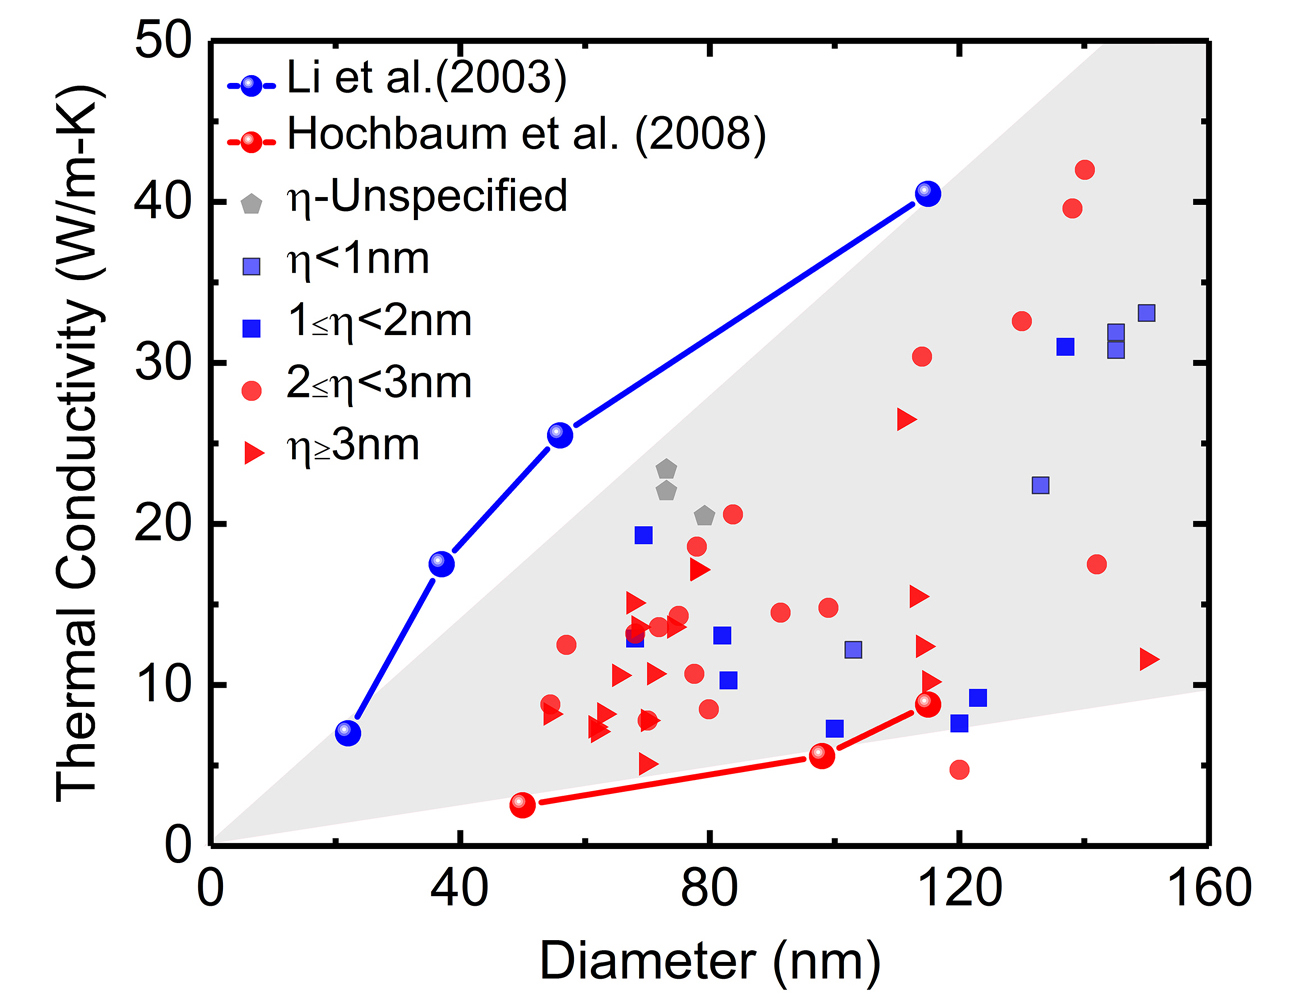
\includegraphics[width=\textwidth]{/ch2/Figure-NW-data.jpg}
	\caption{Current state of room temperature thermal conductivity engineering of nanowires. Thermal conductivity measurements by Li \etal \cite{RN20} on VLS nanowires and Hochbaum \etal \cite{NW_hochbaum} on electroless etched nanowires form an envelope around all other measurements, indicative of an experimental bound on thermal conductivity. Reprinted from ``Phononic Pathways towards Rational Design of Nanowire Heat Conduction" (2019), \textit{Nanotechnology}, Malhotra, A. and Maldovan, M. © IOP Publishing. Reproduced with permission.}
	\label{fig:ch2-nwdatadump}
\end{figure}
\todo{take permission from nanotechnology when published}
We use our surface scattering model (i.e. Beckmann-Kirchhoff formulation with shadowing and angle and momentum dependent phonon scattering) to predict Si and SiGe nanowire thermal conductivities. We find excellent agreement with experimental data-set for the un-etched nanowires of diameters 115 nm, 56 nm, 37 nm \cite{RN20} and 122 nm \cite{RN111} in \Cref{fig:ch2-nw-K}. Since no surface parameters were reported in these experiments, we assume a boundary disorder in the order of Si crystal unit cell (0.4 nm–0.6 nm) and a large enough correlation (10\gls{eta}), compared to those described in etching experiments above, as the wires were not roughened intentionally. Our accurate predictions in un-etched nanowires can be further seen in \Cref{fig:ch2-nw-K}(b) where using the previous assumptions about surface parameters, we also find a good comparison with the experimental values \cite{RN131}. For etched nanowires, the theoretical calculations are in agreement with experiments \cite{RN131,RN130} but the results are slightly larger than the experimental values. The inclusion of an amorphous layer \cite{RN103,RN240} at the boundary (to account for the chemically etched surfaces) is insufficient to account for this reduction. This enhanced reduction could be the result of micro-structural changes which appear as a result of the etching process, as suggested by D. Cahill \cite{RN67}. Additional strains in the silicon crystal introduced due to these changes were not included in our model. We also apply our model to SiGe alloy nanowires and found a similar agreement in \Cref{fig:ch2-nw-K}(c) with the experimental data by taking a higher value of roughness ($\sim 3\times$ Si lattice constant). This is consistent with a previous comparison \cite{RN289} which uses a boundary scattering description with $p = 0$. We note that accounting for changes in relaxation times due to mass difference of point defects \cite{RN289,RN132} and experimental measurements \cite{RN111,RN520} are very sensitive to impurity (alloy) fraction, a slight inaccuracy or mismatch in the reported defect percent against the actual fraction could account for the observed lowered conductivity. Interestingly, for both Si and SiGe nanowires, the BK model provides agreement with experimental results even at low temperatures where the minimum correlation length for strict applicability of the Kirchhoff approximation is expected to be higher. In addition, we predict the thermal conductivity of Si and SiGe nanowires as a function of diameter for different roughness and correlation lengths. The numerical predictions for Si nanowires in \Cref{fig:ch2-nw-K} show how the diameter reduction lowers the thermal conductivity due to the emergence of the non-diffusive (quasi-ballistic) regime of heat conduction where phonon-interface scattering plays an important role. The thermal conductivity is larger for longer correlation lengths, since the probability of phonons undergoing specular reflection is higher due to the larger distance between two surface features. We also predict the thermal conductivities for alloyed nanowires and the diameter dependence for \sige{0.90}{0.10} nanowires shows a similar trend as seen in Si for a quasi-ballistic regime. The magnitude of thermal conductivities in this case, however, are one order of magnitude smaller due to alloying effects. Our model with all the relevant physical parameters and surface scattering phenomena is thus able to predict the thermal conductivities of Si and SiGe nanowires. The presence of crystal strains and/or additional impurities in the samples could lead to lower thermal conductivities (as observed experimentally for etched nanowires).
%---Fig--
\begin{sidewaysfigure}[hbtp]
	\includegraphics[width=\textwidth]{/ch2/Figure-NW-K.jpg}
	\caption{Calculations from our model for (a) Unetched Si nanowires, (b) Unetched and etched Si nanowires and (c) SiGe nanowires for different diameters \gls{dia}. Comparison of the thermal conductivity as a function of temperature from our model shows agreement with experimental measurements (symbols) \cite{RN20,RN131,RN111,RN130,RN116}. (d,e) Theoretical predictions using our approach (BK method with shadowing) for nanowires of different diameters at room temperature with different surface characteristics (roughness and correlation length) for pure Si and SiGe alloys, respectively.}
	\label{fig:ch2-nw-K}
\end{sidewaysfigure}

\subsection{Thin-Films}
% TF
We next use our developed model to predict the thermal conductivities of Si thin films and compare the results with experimental measurements for a wide range of temperatures \gls{T} = 20 K–500 K and film thicknesses \cite{RN217,RN127,RN126,RN128,RN124,RN227,RN274,RN189,RN125}. Similar to experimental surface roughnesses in nanowires, we assume that the surface correlation length is generally in the order of \gls{cl} $\sim$ 10\gls{eta} and take the roughness values in the range of the dimension of the lattice unit cell are a reasonable approximation for un-etched silicon thin films. We note that recent works have assumed a completely diffusive boundary behavior as a good approximation of the surface behavior for most Si thin film samples \cite{RN208,RN217}. In \Cref{fig:ch2-tf-K} the distinction between a fully diffusive boundary and a free Si interface with \gls{eta} $\sim$ 0.5 nm and \gls{cl} $\sim$ 5 nm (i.e. 10\gls{eta}) can be clearly seen. Importantly, we show that the assumption of a fully diffusive boundary is valid only for small thin film dimensions and our accurate model is able to match completely the experimental results. We further note that the incorrect usage of the Ziman formula (with a $\pi^3$ in the exponent instead of $\pi^2$) can lead to overestimation of the scattering at the boundaries \cite{RN208}. Approximating Si nanostructure boundaries as perfectly diffusive is computationally simpler but is expected to be a reasonable assumption only for a reduced range of thicknesses. 
\par We also calculate the thermal conductivity of SiGe alloyed thin films, which are predicted to be an order of magnitude lower than Si thin films. This is the result of the added scattering for short-wavelength (or high-frequency) phonons due to the mass difference between Si and Ge. Variations in surface roughness and correlation lengths can significantly modify the thermal conductivity in these films as shown in \Cref{fig:ch2-tf-K}(c). The thermal conductivity is higher for larger correlation lengths and smaller roughness. This is explained by the fact that the probability of phonons undergoing specular reflection is higher when the surface is smooth and there is more separation between two surface features. The higher correlation length reduces the shadowing effects at the boundary, allowing a larger proportion of the surface to be exposed to phonons. As a result, using our model, precise predictions of the thermal conductivity can be made based on quantifiable surface characteristics (i.e., surface roughness and correlation lengths), which are critical physical parameters influencing thermal transport. 
\par The variation of thermal conductivity with surface roughness for different thicknesses and fixed correlation length is shown in \Cref{fig:ch2-tf-K}(d). The increase in surface roughness does not affect the thin-film thermal conductivity beyond a certain value ($\eta>$ 1.5 nm and 2 nm for Si and \sige{0.90}{0.10} thin-films, respectively) which indicates the complete onset of diffuse surface scattering. In an experimental setup, however, the roughening/etching of semiconductor surfaces may introduce additional strains or dislocations \cite{RN67} or cause the oxide layer formation along the interface \cite{RN393}, which can additionally affect the thermal conductivity.
%Figure TF K
\begin{figure}[hbt]
	\includegraphics[width=\textwidth]{/ch2/Figure-TF-K.jpg}
	\caption{Thermal conductivity predictions and comparison with experimental measurements \cite{RN274,RN189,RN127,RN126,RN217,RN128,RN124,RN227,RN125}. (a) Thermal conductivity as a function of temperature for Si and SiGe thin films of different thicknesses. Predicted thermal conductivity of (b) Si and (c) \sige{0.80}{0.20} thin films as a function of thickness for different surface conditions. (d) Thermal conductivity as a function of surface roughness for Si and \sige{0.90}{0.10} thin-films of thickness 500 nm (black squares), 100 nm (red-circles) and 20 nm(blue-triangles) at room temperature. The correlation length is \gls{cl} = 10\gls{eta}. Arrows indicate the onset of complete diffuse scattering.}
	\label{fig:ch2-tf-K}
\end{figure}
%SPECTRA SECTION
\newpage
\section{Predictions of Thermal Spectra}
\label{sec:pred_thermalspectra}
A current fundamental challenge in nanoscale heat transport is to precisely predict how much heat is carried by phonons with different wavelengths and mean-free-paths, i.e. normalized cumulative thermal conductivity or thermal spectra. The thermal conductivity accumulation function (i.e., the thermal energy distribution or heat spectra) as a function of wavelength \gls{wl} (or mean-free-path \gls{mfp}) is the proportion of the heat carried by phonons with wavelengths smaller than \gls{wl} (or \gls{mfp}), and provides the distribution of the heat among phonons with different wavelengths and mean-free-paths. Access to such thermal energy distribution would allow to explain the existence of ballistic versus diffuse regimes, phonon confinement, and wave interference effects \cite{RN362}. In recent years, significant efforts have been conducted to reconstruct the mean-free-path accumulative thermal conductivity of bulk materials via the combination of the suppression function and experimental measurements \cite{RN236,RN273,RN217,RN129}. This recently proposed experimental route to obtain heat spectra can be readily compared to DFT-based numerical calculations \cite{stokes_bulkSi_tau}. Importantly, if such deep knowledge of fundamental phonon transport properties in bulk materials is to be routinely extended to nanostructures, an accurate description of phonon surface scattering is critically needed beyond the standard assumption of complete diffuse scattering. In particular, a major research question that needs to be answered is the precise determination of the proportion of thermal phonons that are specularly and diffusively scattered at surfaces. The answer to this question has remained limited under the empirical approaches relying on overall relaxation times or using a constant value for the surface specularity \gls{p} (i.e. the proportion of specularly reflected phonons) without accounting for underlying physics of phonons and surfaces. The accurate prediction of thermal spectra using the described model incorporating both surface characteristics and incident phonon properties is the central goal of this section.
\subsection{Methodology}
In order to calculate thermal spectra as a function of frequency \gls{freq}, we apply a numerical approach where we create multiple \textit{bins} spanning 0.2 THz each. Similar bins of 10 nm and 2 nm were used for thermal spectra as a function of mean-free-path \gls{mfp} and wavelength \gls{wl}, respectively. Based on these bins, we numerically determine the wave-vectors \gls{k} for all polarizations that lead to frequencies (or mean-free-paths or wavelengths) lying in the bin. This approach of binning wave-vectors allow for limiting the calculation to desired \gls{freq} (or \gls{mfp} or \gls{wl}) ranges. The spectral contribution of phonons belonging to a particular wave-vector bin to overall thermal transport is evaluated by using,
\begin{equation}
\mathrm{Spectra} =\dfrac{\kappa_\mathrm{bin}}{\kappa_\mathrm{total}}\times 100\% = \dfrac{\sum_{\vec{k'}\in\,\mathrm{bin}} \hbar\omega_{\mathbf{k'}}\dfrac{\partial f^{BE}}{\partial T}v_{\mathbf{k'}}\ell_{\mathbf{k'}}}{\sum_{\forall\,\vec{k}} \hbar\omega_{\mathbf{k}}\dfrac{\partial f^{BE}}{\partial T}v_{\mathbf{k}}\ell_{\mathbf{k}}}\times 100\%
\end{equation}

\subsection{Bulk Si Spectra}
%Spectra Bulk
\begin{figure}[hbt]
  \centering \includegraphics[width=\textwidth]{/ch2/Figure-NW-Spectra0.jpg}
  \caption{(a) Comparisons between mean-free-path heat spectrum (normalized cumulative conductivity) for bulk Si from our calculations, first principle approaches \cite{stokes_bulkSi_tau}, and reconstruction from experiments \cite{RN273,RN129,RN217}. (b) Calculated wavelength heat spectrum for bulk Si and SiGe alloy, and (c) Calculated mean-free-path heat spectrum for \sige{0.90}{0.10} nanowire and the reconstructed spectrum using Ziman’s formula for \gls{eta} = 0.1 nm \cite{RN129}.}
  \label{fig:ch2-nw-spectra-0}
\end{figure}
\par We first predict the heat spectrum of bulk Si and SiGe materials and compare it against computationally expensive DFT calculations \cite{stokes_bulkSi_tau} and more recent experimental approaches that reconstruct the conductivity measurement into a heat spectrum as a function of phonon mean-free-path by use of a suppression function \cite{RN273,RN129,RN217}. We note the strong agreement between all approaches in \Cref{fig:ch2-nw-spectra-0}(a) enabling a prediction about the bulk silicon mean-free-path heat spectrum with certainty. Another important feature that needs to be considered is the thermal phonon wavelengths. Since the experimental reconstruction approach for the heat spectrum can provide only the mean-free-path spectra, we are restricted to compare our bulk calculations to DFT in \Cref{fig:ch2-nw-spectra-0}(b). Once again, our calculations for bulk silicon is in close agreement with DFT calculations \cite{stokes_bulkSi_tau}. In addition, we present our predictions for the heat spectrum of bulk \sige{0.90}{0.10} alloy. As mentioned previously, with the introduction of Ge atoms in the matrix, the spectrum shows a marked change towards longer phonon wavelengths (and larger mean-free-paths). It can thus be postulated that any change from a pure bulk structure (e.g. defects, interfaces etc.) affects both the thermal conductivity and the phonon heat spectrum. 
\par For the case of nanowires in \Cref{fig:ch2-nw-spectra-0}(c), the reconstructed heat spectrum as a function of mean-free-paths is available only for a \sige{0.90}{0.10} \cite{RN129}. This reconstruction is based on a Ziman formulation (normal incidence) for phonon boundary scattering which is expected to overestimate the effect of the boundaries \cite{ownNW}. Our results using the BTE formulation with the same assumptions show a close agreement with this reconstructed mean-free-path. Next, we look at the details of the thermal spectra in nanowires using our model.
\subsection{Nanowires}
Using our surface scattering model, we calculate the wavelength and mean-free-path heat spectra for Si nanowires for different diameters, surface roughness, and correlation lengths. \Cref{fig:ch2-nw-spectra-1} quantitatively shows how the introduction of rough boundaries strongly shifts the nanowire heat spectrum to shorter wavelengths and shorter mean-free-paths with respect to bulk silicon. For example, in bulk Si, the dominant heat carrying phonons (10–90\%) have a wavelength \gls{wl} $\sim$ 0.9–10 nm while in a nanowire of 100 nm diameter [\Cref{fig:ch2-nw-spectra-1}(a)], the dominant spectrum shifts to 0.6–2.5 nm range. A similar effect is seen in the mean-free-path spectrum which shows a marked shift from 0.1 \si{\micro}m–100 \si{\micro}m (bulk) to 15–200 nm (nanowire) [\Cref{fig:ch2-nw-spectra-1}(b)]. Such a spectrum shift is a direct consequence of the transition from bulk to a nanowire structure. In general, with the introduction of the boundaries, phonons with longer mean-free-paths (and larger wavelengths) can interact more strongly with the boundaries than those with shorter mean-free-paths. Since the roughened boundary provides an additional scattering mechanism, these phonons scatter more and achieve local equilibrium. The additional boundary scattering not only reduces the nanowire thermal conductivity as compared to bulk, but also strongly modifies the phonon heat spectra. \Cref{fig:ch2-nw-spectra-1} also shows the marked shift to shorter wavelengths and mean-free-paths with increasing surface roughness. By increasing the roughness from 0.5 nm to 1.5 nm, there is a shift to shorter wavelengths and smaller mean-free-paths in the thermal phonon distribution caused by the enhanced diffuse scattering.
%Spectra NW 1
\begin{figure}[hbtp]
  \centering 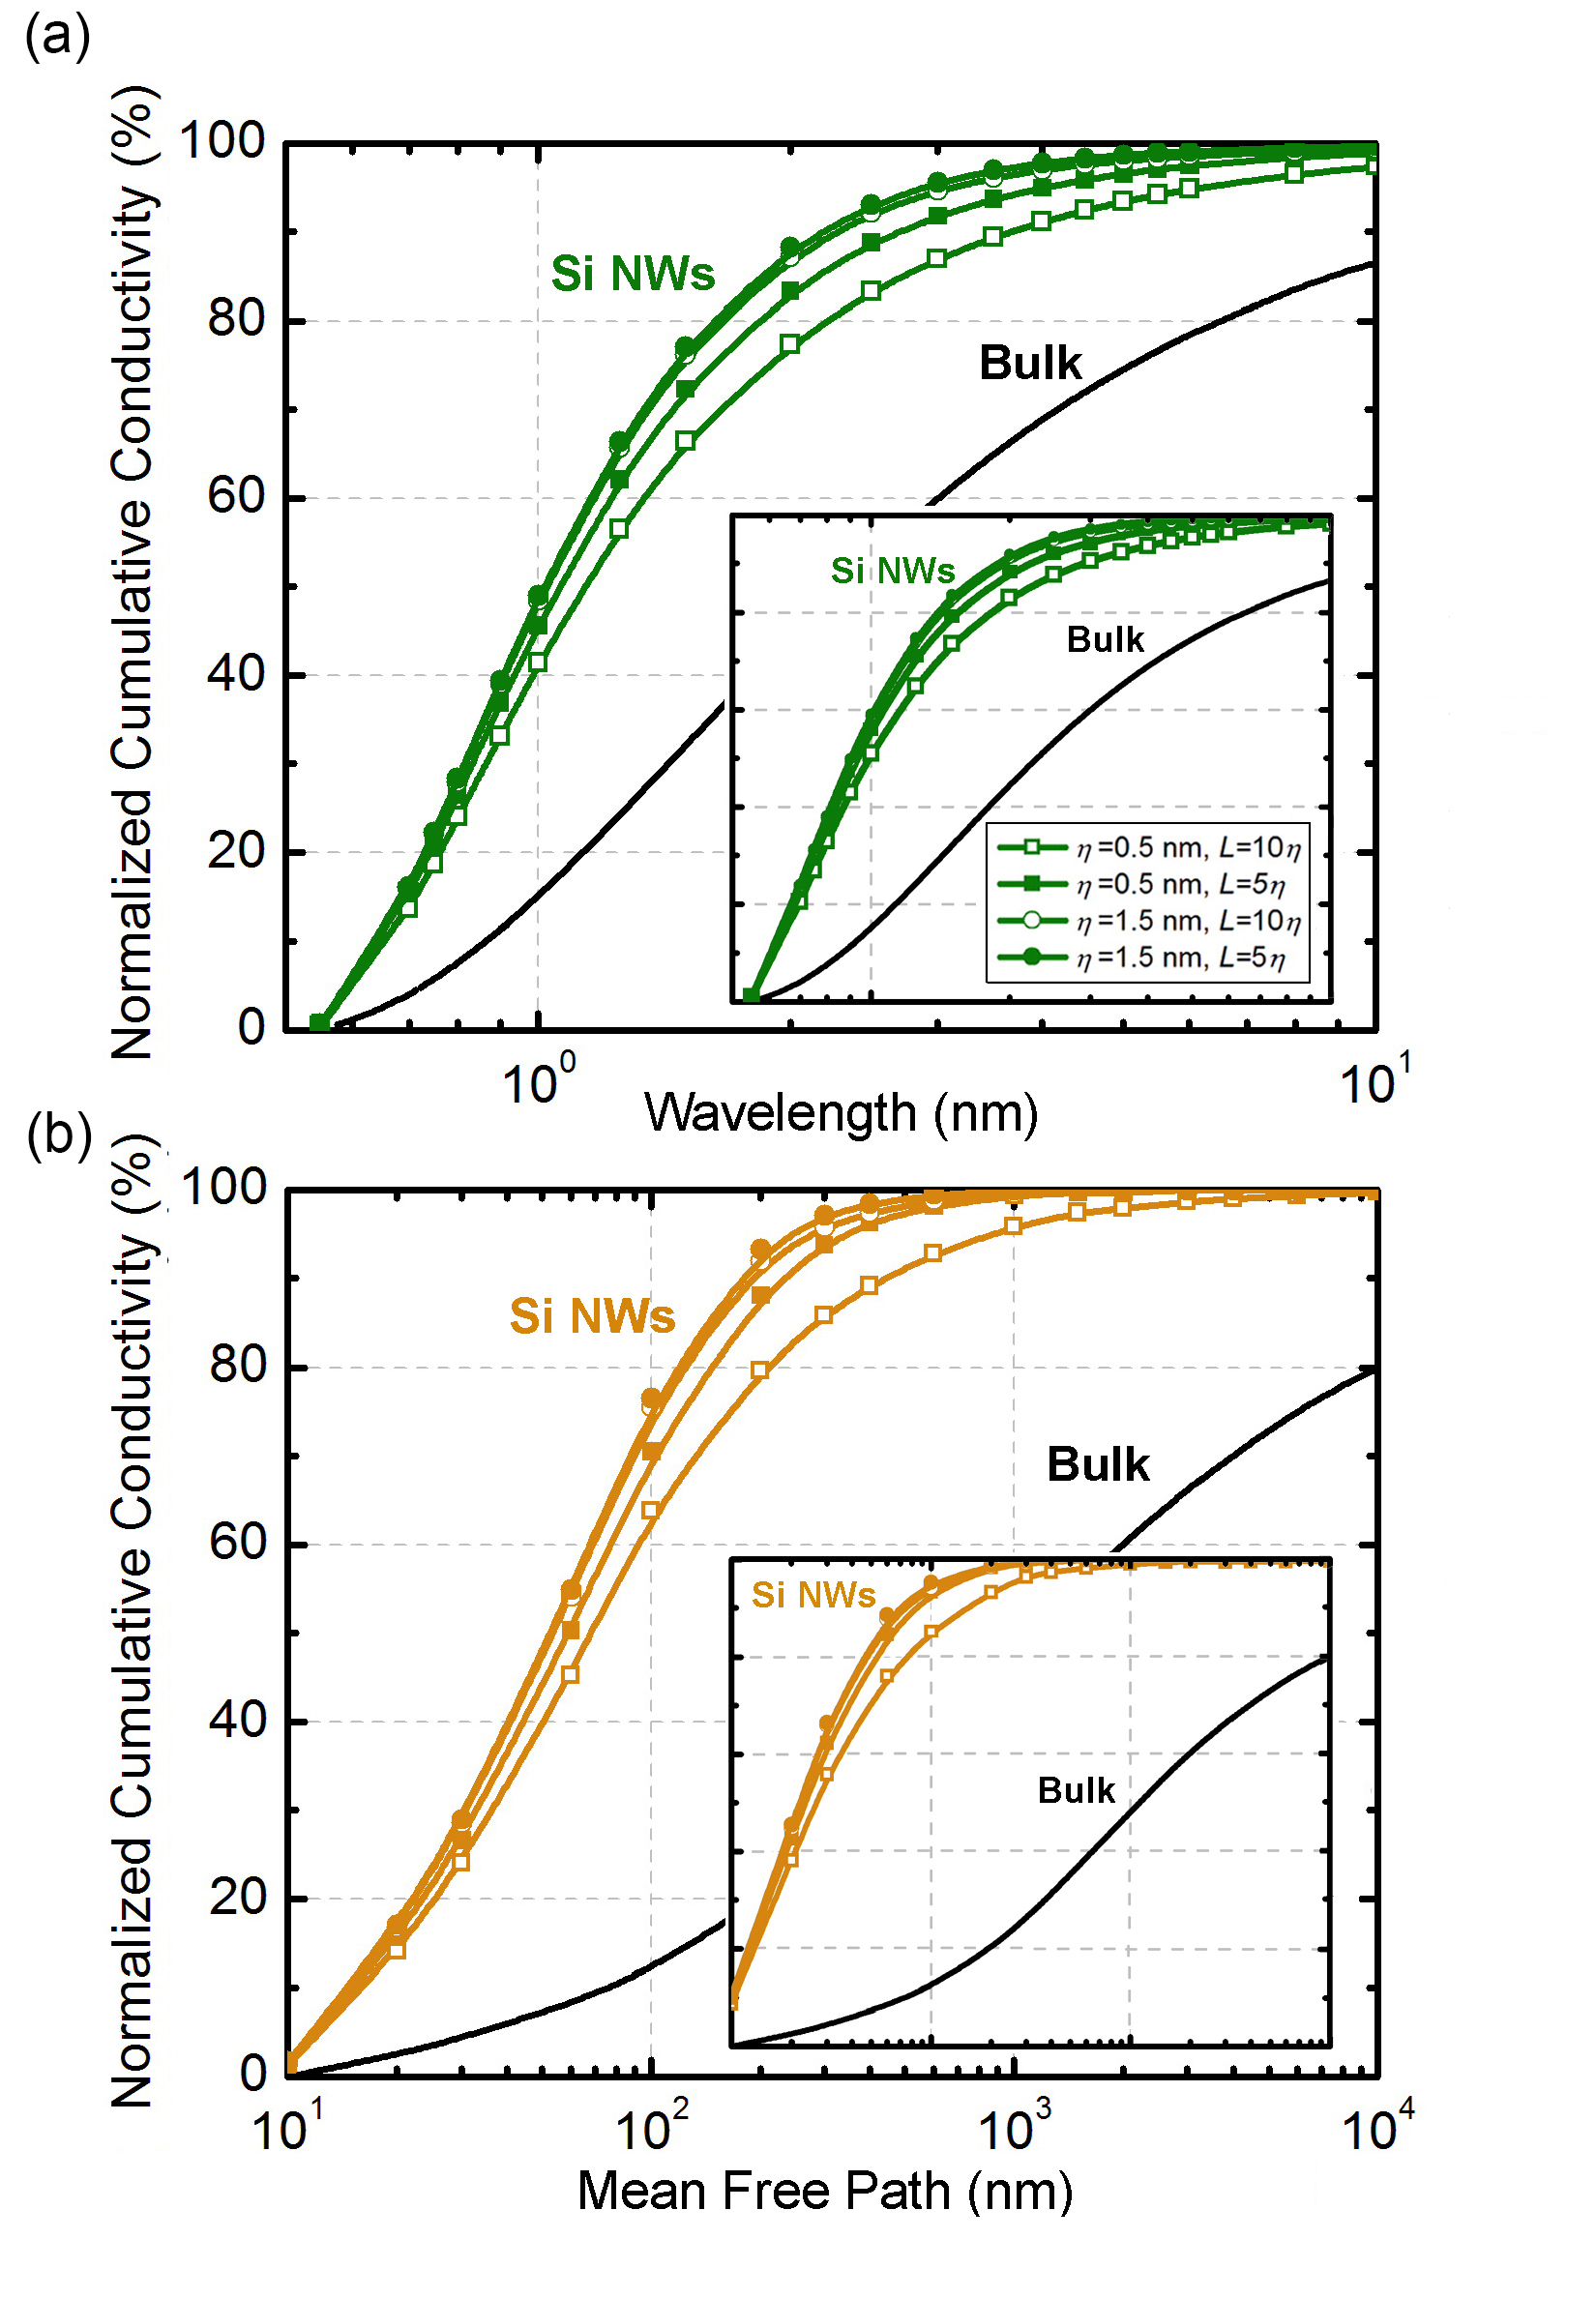
\includegraphics[width=0.85\textwidth]{/ch2/Figure-NW-Spectra1.jpg}
  \caption{Numerical prediction for heat spectra of silicon nanowires at room temperature. (a) Wavelength spectrum and (b) Mean-free-path spectrum for diameter \gls{dia} = 100 nm. Inset shows the calculations for \gls{dia} = 30 nm. Heat spectra are plotted for different roughness \gls{eta} and correlations lengths \gls{cl}. Bulk silicon spectrum is also shown as reference.}
  \label{fig:ch2-nw-spectra-1}
\end{figure} 
\par We also investigated the effects of the surface correlation lengths on the heat spectra. For a given surface roughness, a smaller correlation length enhances the impact of scattering at the boundary. This is seen as an enhanced shift in the heat spectra towards shorter mean-free-paths and smaller wavelengths (i.e. blue-shift). For example, in a Si nanowire with \gls{dia} = 100 nm and surface roughness \gls{eta} = 0.5 nm, phonons with wavelengths shorter than 2 nm carry $\sim$77\% of total heat if the correlation length is \gls{cl} = 5 nm. However, this proportion increases to 83\% if the correlation length is shortened to \gls{cl} = 2.5 nm. Similarly, in the case of the mean-free-path spectrum, phonons with mean-free-paths less than 200 nm carry 79\% of heat if \gls{cl} = 5 nm. Reducing this correlation length to \gls{cl} = 2.5 nm increases the heat carried by these phonons to 88\%. Importantly, these detailed modifications of the heat spectra cannot be predicted by approximate boundary scattering models. We note that the surface correlation length provides a statistical quantification of the distance between repeated roughness features. The frequent appearance of “hills and valleys” for a surface with small correlation length contributes towards more shadowing, modifying the probability of specular reflection. The enhanced shadowing for small correlations lengths increases the overall boundary effect causing the nanowire heat spectra to be dominated by shorter wavelength and smaller mean-free-paths. We also performed a comparison of the previous results with the spectra for a smaller nanowire (\gls{dia} = 30 nm) and found an additional shift of the spectrum to lower wavelength and mean-free-paths [\Cref{fig:ch2-nw-spectra-1}, insets]. This is consistent since the effects of boundary scattering are slightly more pronounced in a smaller diameter nanowire because a larger range of phonons can interact strongly with the nanowire surfaces.

It is important to note that, in contrast to surface scattering, the addition of mass-defects in the Si crystalline lattice in the form of Ge atoms is an effective mechanism to reduce the thermal conductivity by scattering phonons with shorter wavelengths and smaller mean-free-paths \cite{RN132,RN98}. For this reason, the dominant wavelengths and the mean-free-paths in low Ge concentration SiGe alloys are higher as compared to pure silicon. This means that while surface scattering shifts the bulk heat spectra to short wavelengths, alloy scattering shifts the bulk spectra to long wavelengths. We found that in a SiGe nanowire, where the spectra are already shifted in comparison with Si, the effect of boundary scattering is again seen by a transition to shorter mean-free-paths and wavelengths (i.e. blue-shift) [\Cref{fig:ch2-nw-spectra-2}]. This is similarly explained by the ability of the phonons with longer wavelengths (and mean-free-paths) to “see” the boundaries more effectively and have a higher interfacial interaction. An interesting property of the alloyed nanowire spectrum is the larger and broader ranges of the dominant region. If we consider the range of the middle 80\% of the heat spectrum (10–90\% of heat), the phonon mean-free-paths lie in the range of 5 nm–3 \si{\micro}m while the wavelengths are in the range of 1–20 nm. The exact value certainly depends on the roughness and correlation length of the surface under consideration. This is significantly larger and wider than the ranges seen for Si nanowires. These spectrum features are a consequence of the combined effects of alloyed scattering and boundary scattering. We note that while Ge atoms are very effective in scattering short mean-free-path (and small wavelength) phonons, boundaries are effective in interacting with phonons of larger mean-free-paths (and longer wavelengths). This leaves a larger and relatively broader “middle” range as the major conductor of the heat in the SiGe alloyed nanowires. The effects of reducing the correlation lengths via the enhanced shadowing of nanowire surface is still observed similarly to Si nanowires.
%Spectra NW 2
\begin{figure}[hbtp]
  \centering 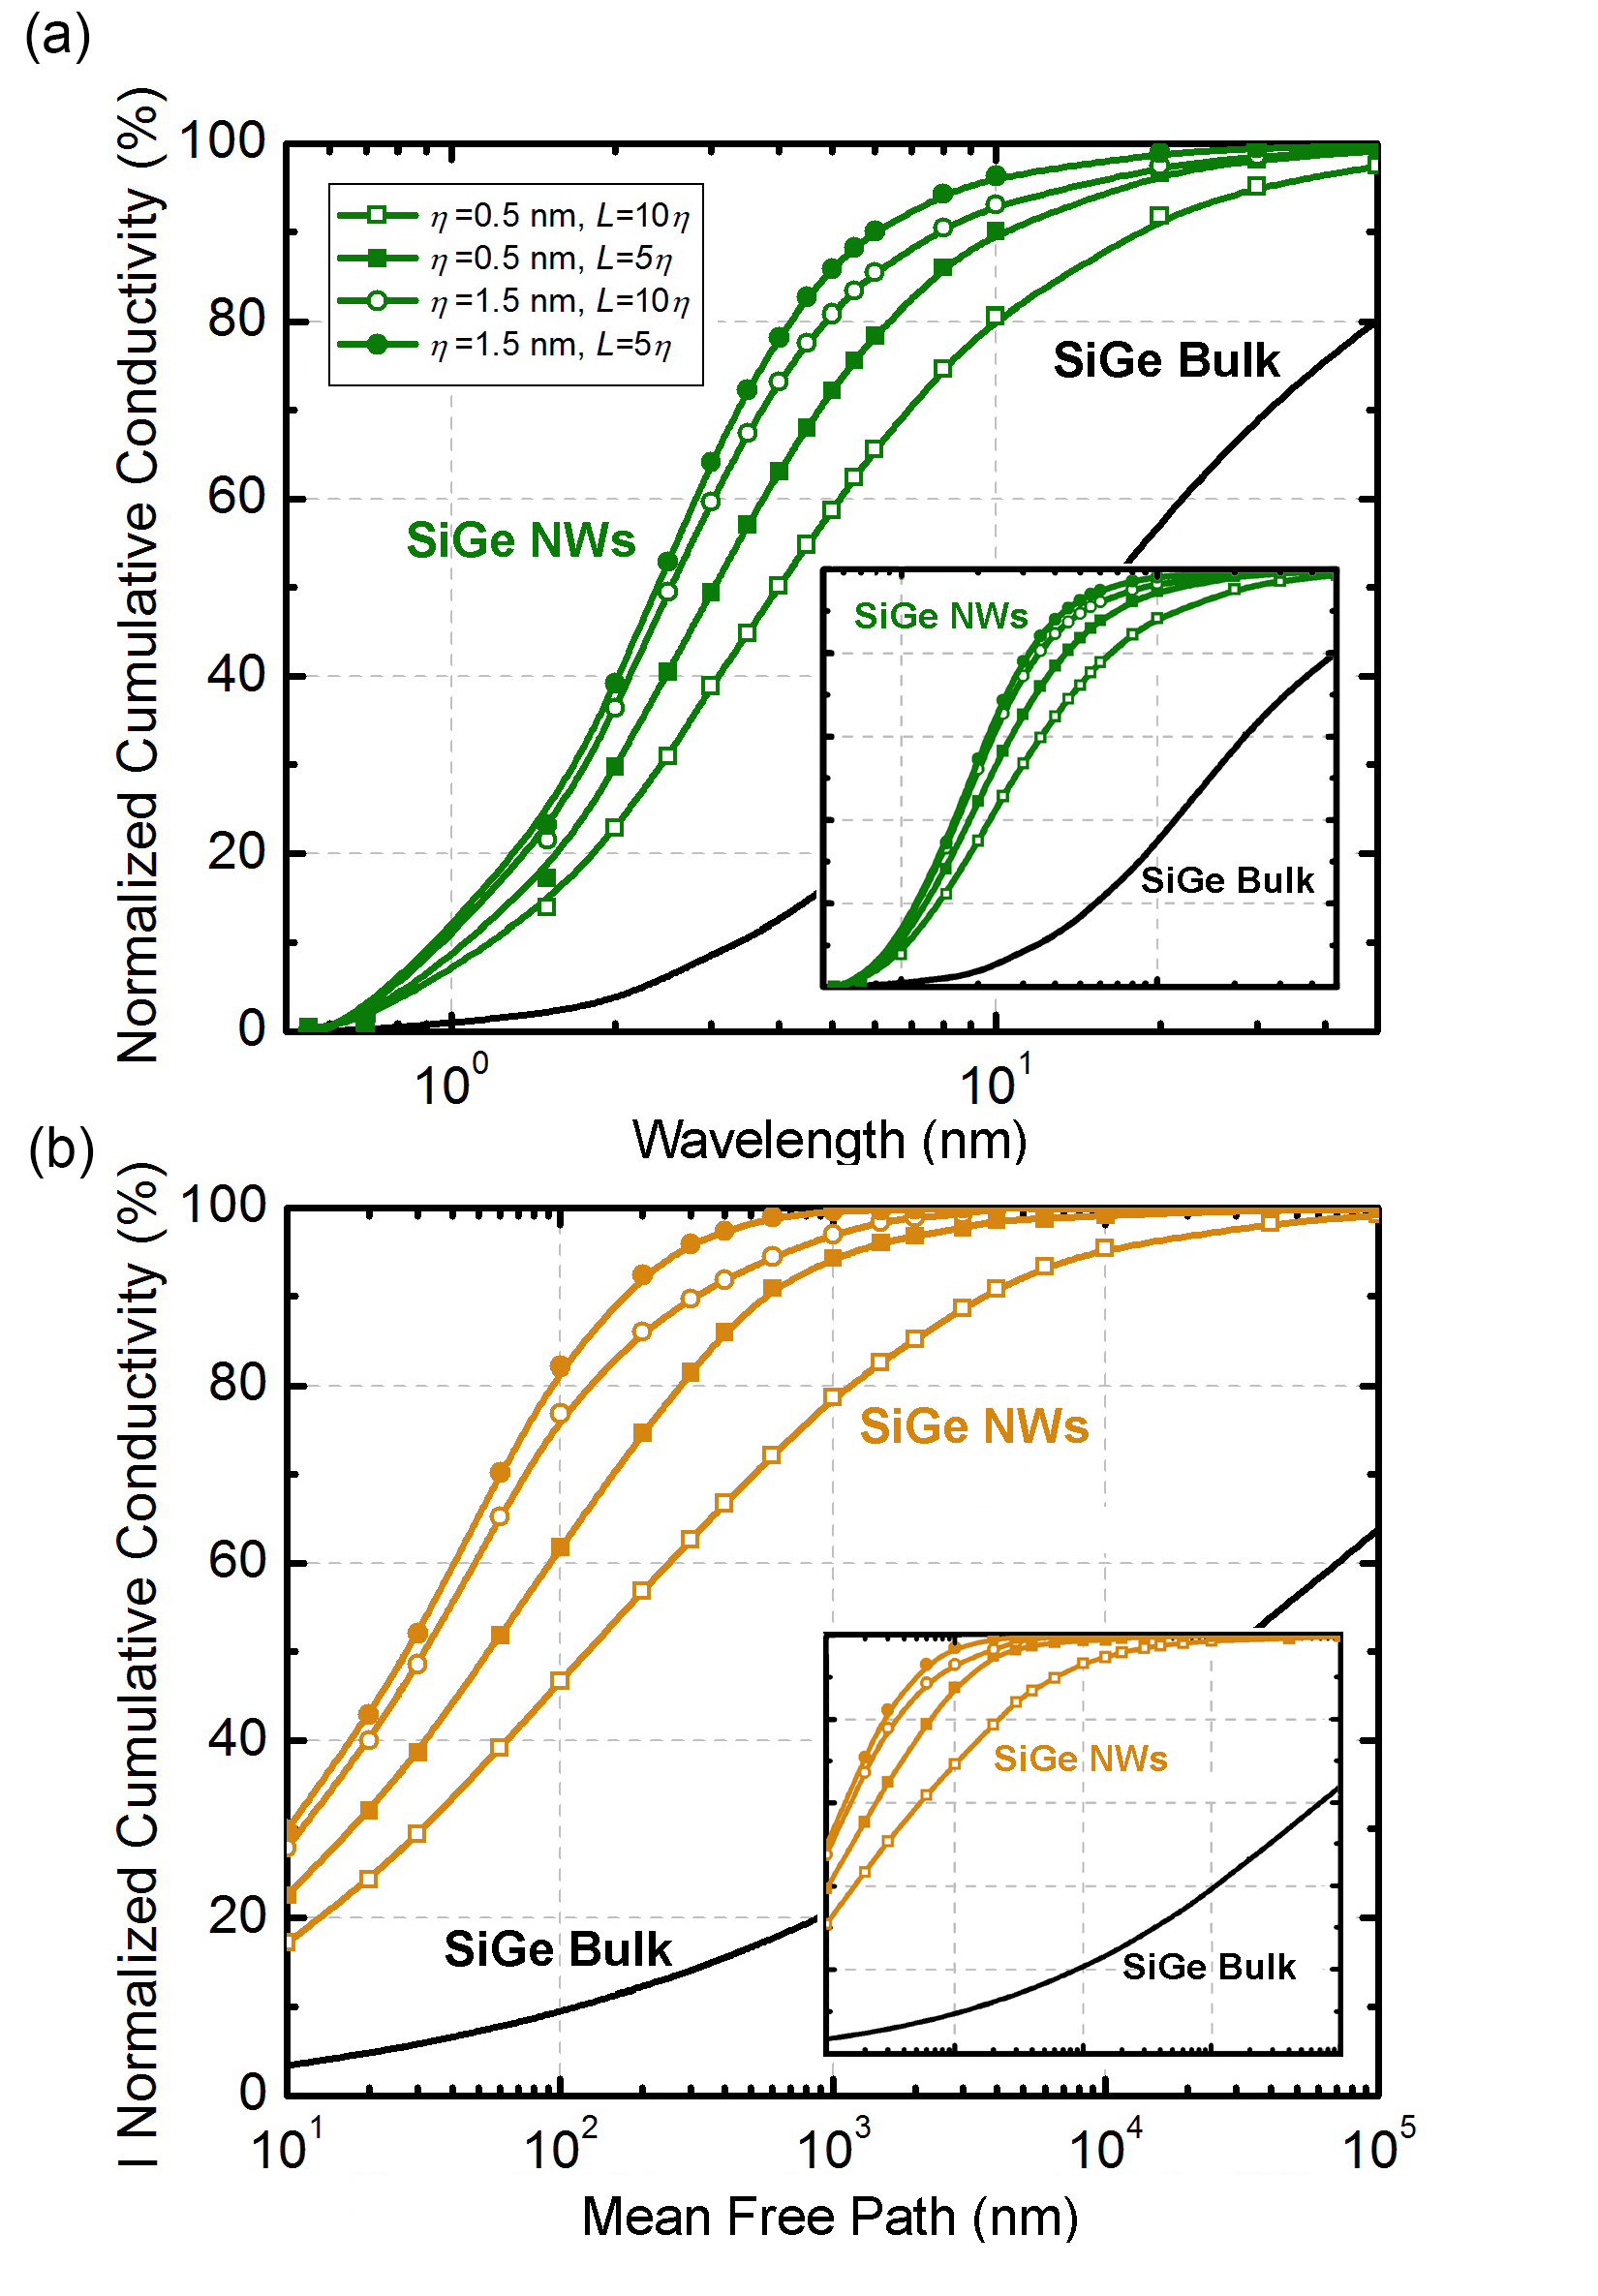
\includegraphics[width=0.85\textwidth]{/ch2/Figure-NW-Spectra2.jpg}
  \caption{Wavelength heat spectra for \sige{0.90}{0.10} alloy nanowires at room temperature for (a) \gls{dia} = 100 nm (and inset for \gls{dia} = 30 nm). (b) Mean-free-path heat spectrum for nanowire diameters \gls{dia} = 100 nm and 30 nm.}
  \label{fig:ch2-nw-spectra-2}
\end{figure}

%------TF------
\subsection{Thin-Films}
Using our model, we predict the thermal conductivity accumulation function for silicon thin films of 100 nm and 30 nm thickness and study the effects of surface roughness by choosing two vastly varying surface conditions -- a smooth (\gls{eta} = 0.5 nm, \gls{cl} = 10\gls{eta}) and a rough (\gls{eta} = 1.5 nm, \gls{cl} = 3\gls{eta}) interface, respectively [\Cref{fig:ch2-tf-spectra-1}]. We find that the introduction of different interfaces can differently modify the accumulation function to shorter wavelengths and shorter mean-free-paths with respect to bulk silicon. For example, in bulk Si, the dominant heat-carrying phonons (20\%–80\%) have a mean-free-path of 0.2 \si{\micro}m–10 \si{\micro}m (wavelengths 1–7 nm). The introduction of a smooth boundary in a 100 nm thin film, however, alters these ranges to 40 nm–420 nm (0.85–2.5 nm) and a rough interface modifies these to 35 nm–300 nm (0.80 nm–2 nm). The observed shift of the accumulation functions to shorter wavelengths and mean-free-paths is the consequence of greater diffuse surface scattering of phonons. Phonons with longer mean-free-paths can effectively interact with the rough surface, while the smaller correlation length creates a surface with enhanced shadowing. This combination of increased roughness and shortened correlation length leads to phonons with shorter mean-free-paths (and wavelengths) to become dominant thermal carriers. These trends in the accumulation function are also observed in the thinner 30 nm silicon thin film [\Cref{fig:ch2-tf-spectra-1}, insets].
%Spectra TF 1
\begin{figure}[hbt]
  \centering \includegraphics[width=\textwidth]{/ch2/Figure-TF-Spectra1.jpg}
  \caption{Numerical predictions for the thermal conductivity accumulation functions for Si and SiGe thin films at room temperature. (a) Wavelength spectrum and (b) Mean-free-path spectrum for thickness \gls{t} = 100 nm. Insets, show the corresponding calculations for \gls{t} = 30 nm. Accumulation functions are plotted for different roughness \gls{eta} and correlations lengths \gls{cl}. Accumulation functions for \sige{0.90}{0.10} alloyed thin films are also calculated as a function of phonon (c) Wavelength and (d) Mean-free-paths. Black solid lines show the bulk thermal conductivity accumulation as reference.}
  \label{fig:ch2-tf-spectra-1}
\end{figure}
\par We also consider SiGe alloy films and predict the thermal conductivity accumulation under different surface conditions. It is important to note that there is a significant modification in the bulk \sige{0.90}{0.10} energy spectra (with respect to bulk Si) due to the mass-difference scattering generated by atomically heavier Ge atoms, which are effective in scattering high frequency phonons. This results in the middle 60\% of the energy to be carried by phonons of mean-free-path 1 \si{\micro}m–500 \si{\micro}m (wavelength 6–60 nm) in bulk SiGe. For the 100 nm SiGe thin film, the additional phonon boundary scattering creates a dominant region of phonons with mean-free-paths ranging from 25 nm–1500 nm (2 nm–10 nm) for a smooth boundary and 10 nm–250 nm (1.5 nm–5 nm) for a rough boundary. Effect of temperature on the thermal conductivity accumulation function is also explored in \Cref{fig:ch2-tf-spectra-2} for Si thin film (\sige{0.90}{0.10} in inset) of thickness 100 nm with smooth (\gls{eta} = 0.5 nm, \gls{cl} = 10\gls{eta}) and rough (\gls{eta} = 1.5 nm, \gls{cl} = 3\gls{eta}) interfaces. We note that the accumulation functions are determined by two mechanisms acting on different phonon wavelengths -- increase in temperature excites short wavelength phonons, while surfaces primarily scatter large wavelength (and mean-free-path) phonons, suppressing their contribution [\Cref{fig:ch2-tf-spectra-2}(a)]. In addition, in SiGe alloys, mass difference scattering promotes large-wavelength phonons as dominant carriers, allowing the boundary scattering mechanism to act on a broader range of heat-carrying phonons [\Cref{fig:ch2-tf-spectra-2}(b)]. 
%Spectra TF 2
\begin{figure}[hbt]
  \centering 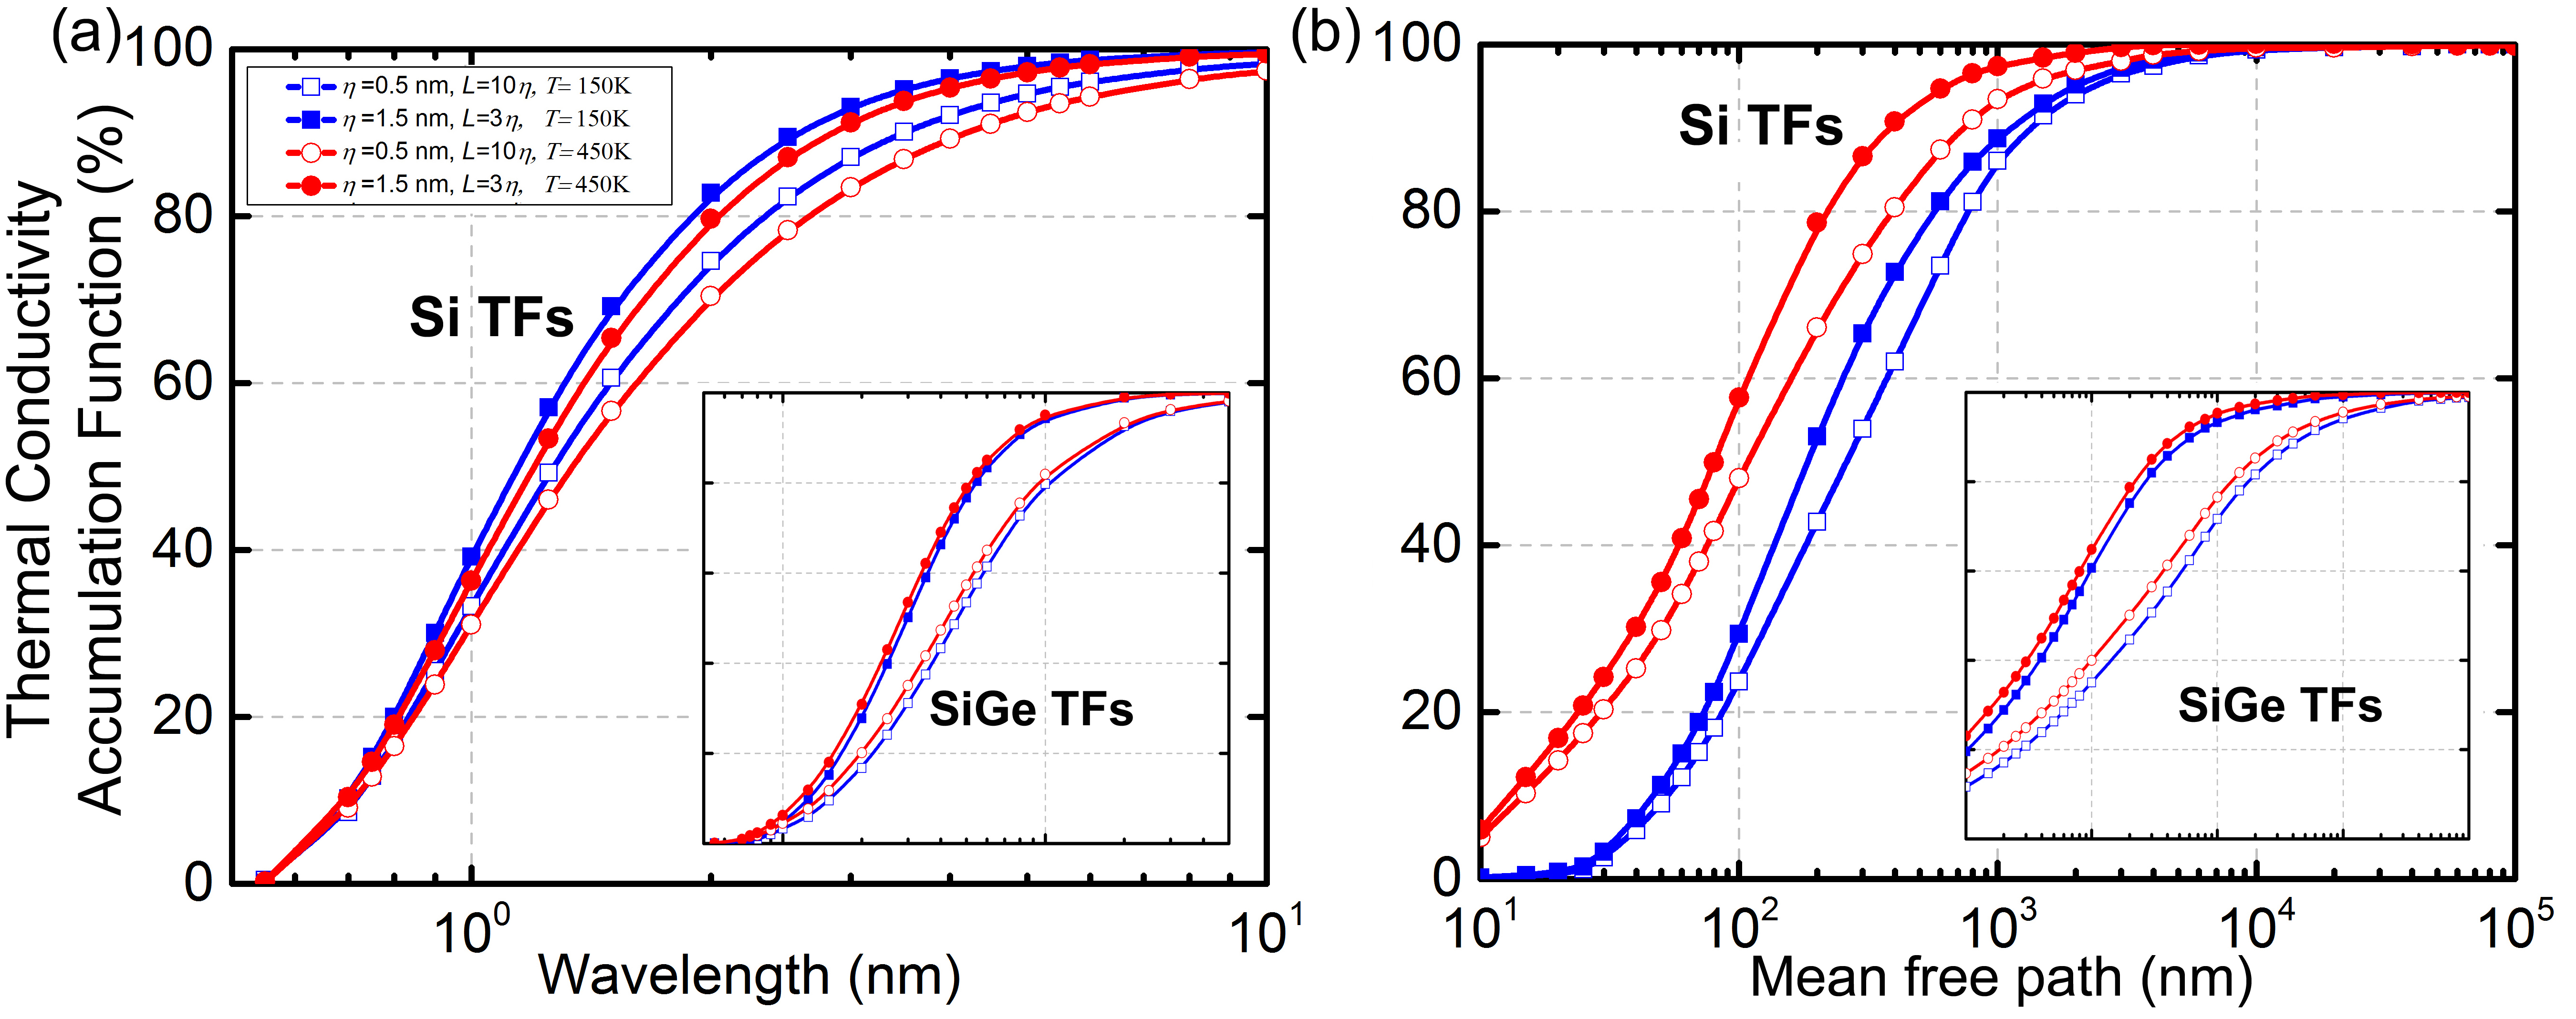
\includegraphics[width=\textwidth]{/ch2/Figure-TF-Spectra2.jpg}
  \caption{Dependence of the accumulation functions on temperature (450 K in red lines and 150 K in blue lines) for Si thin film (\sige{0.90}{0.10}, insets) of thickness \gls{t} = 100nm and rough (\gls{eta} = 1.5 nm, \gls{cl} = 3\gls{eta} filled symbols) and smooth (\gls{eta} = 0.5 nm, \gls{cl} = 10\gls{eta}, open symbols) boundaries. The accumulation function is presented across phonon (a) wavelengths and (b) mean-free-paths.}
  \label{fig:ch2-tf-spectra-2}
\end{figure}
\par These results show how the specific surface properties and temperatures can significantly modify the thermal conductivity accumulation, opening a way forward to the rational design of the semiconductor-air interfaces, which can be utilized to tailor the desired thermal transport properties in nanostructures. This principle of purposely modified phonon transport properties is illustrated in \Cref{fig:ch2-tf-spectra-3}, where surface properties, thicknesses, and alloying are used to modulate the thermal energy distribution of silicon. Introduction of alloy atoms creates a shift towards a large-wavelength energy spectra (i.e., red-shift). A film with a perfectly smooth surface would exhibit the energy spectra of the bulk alloy but surface roughening and thickness variations can be made to blue-shift towards shorter wavelength spectra. A rougher interface and a smaller film size both favor blue-shift of wavelength spectra as the effects of boundary scattering are more pronounced. As a result, the amount of thermal energy carried by phonons with wavelengths in the range 1–10 nm can be designed to be from $\sim$ 30\% to 90\%.
%Spectra TF 3
\begin{figure}[hbt]
  \centering 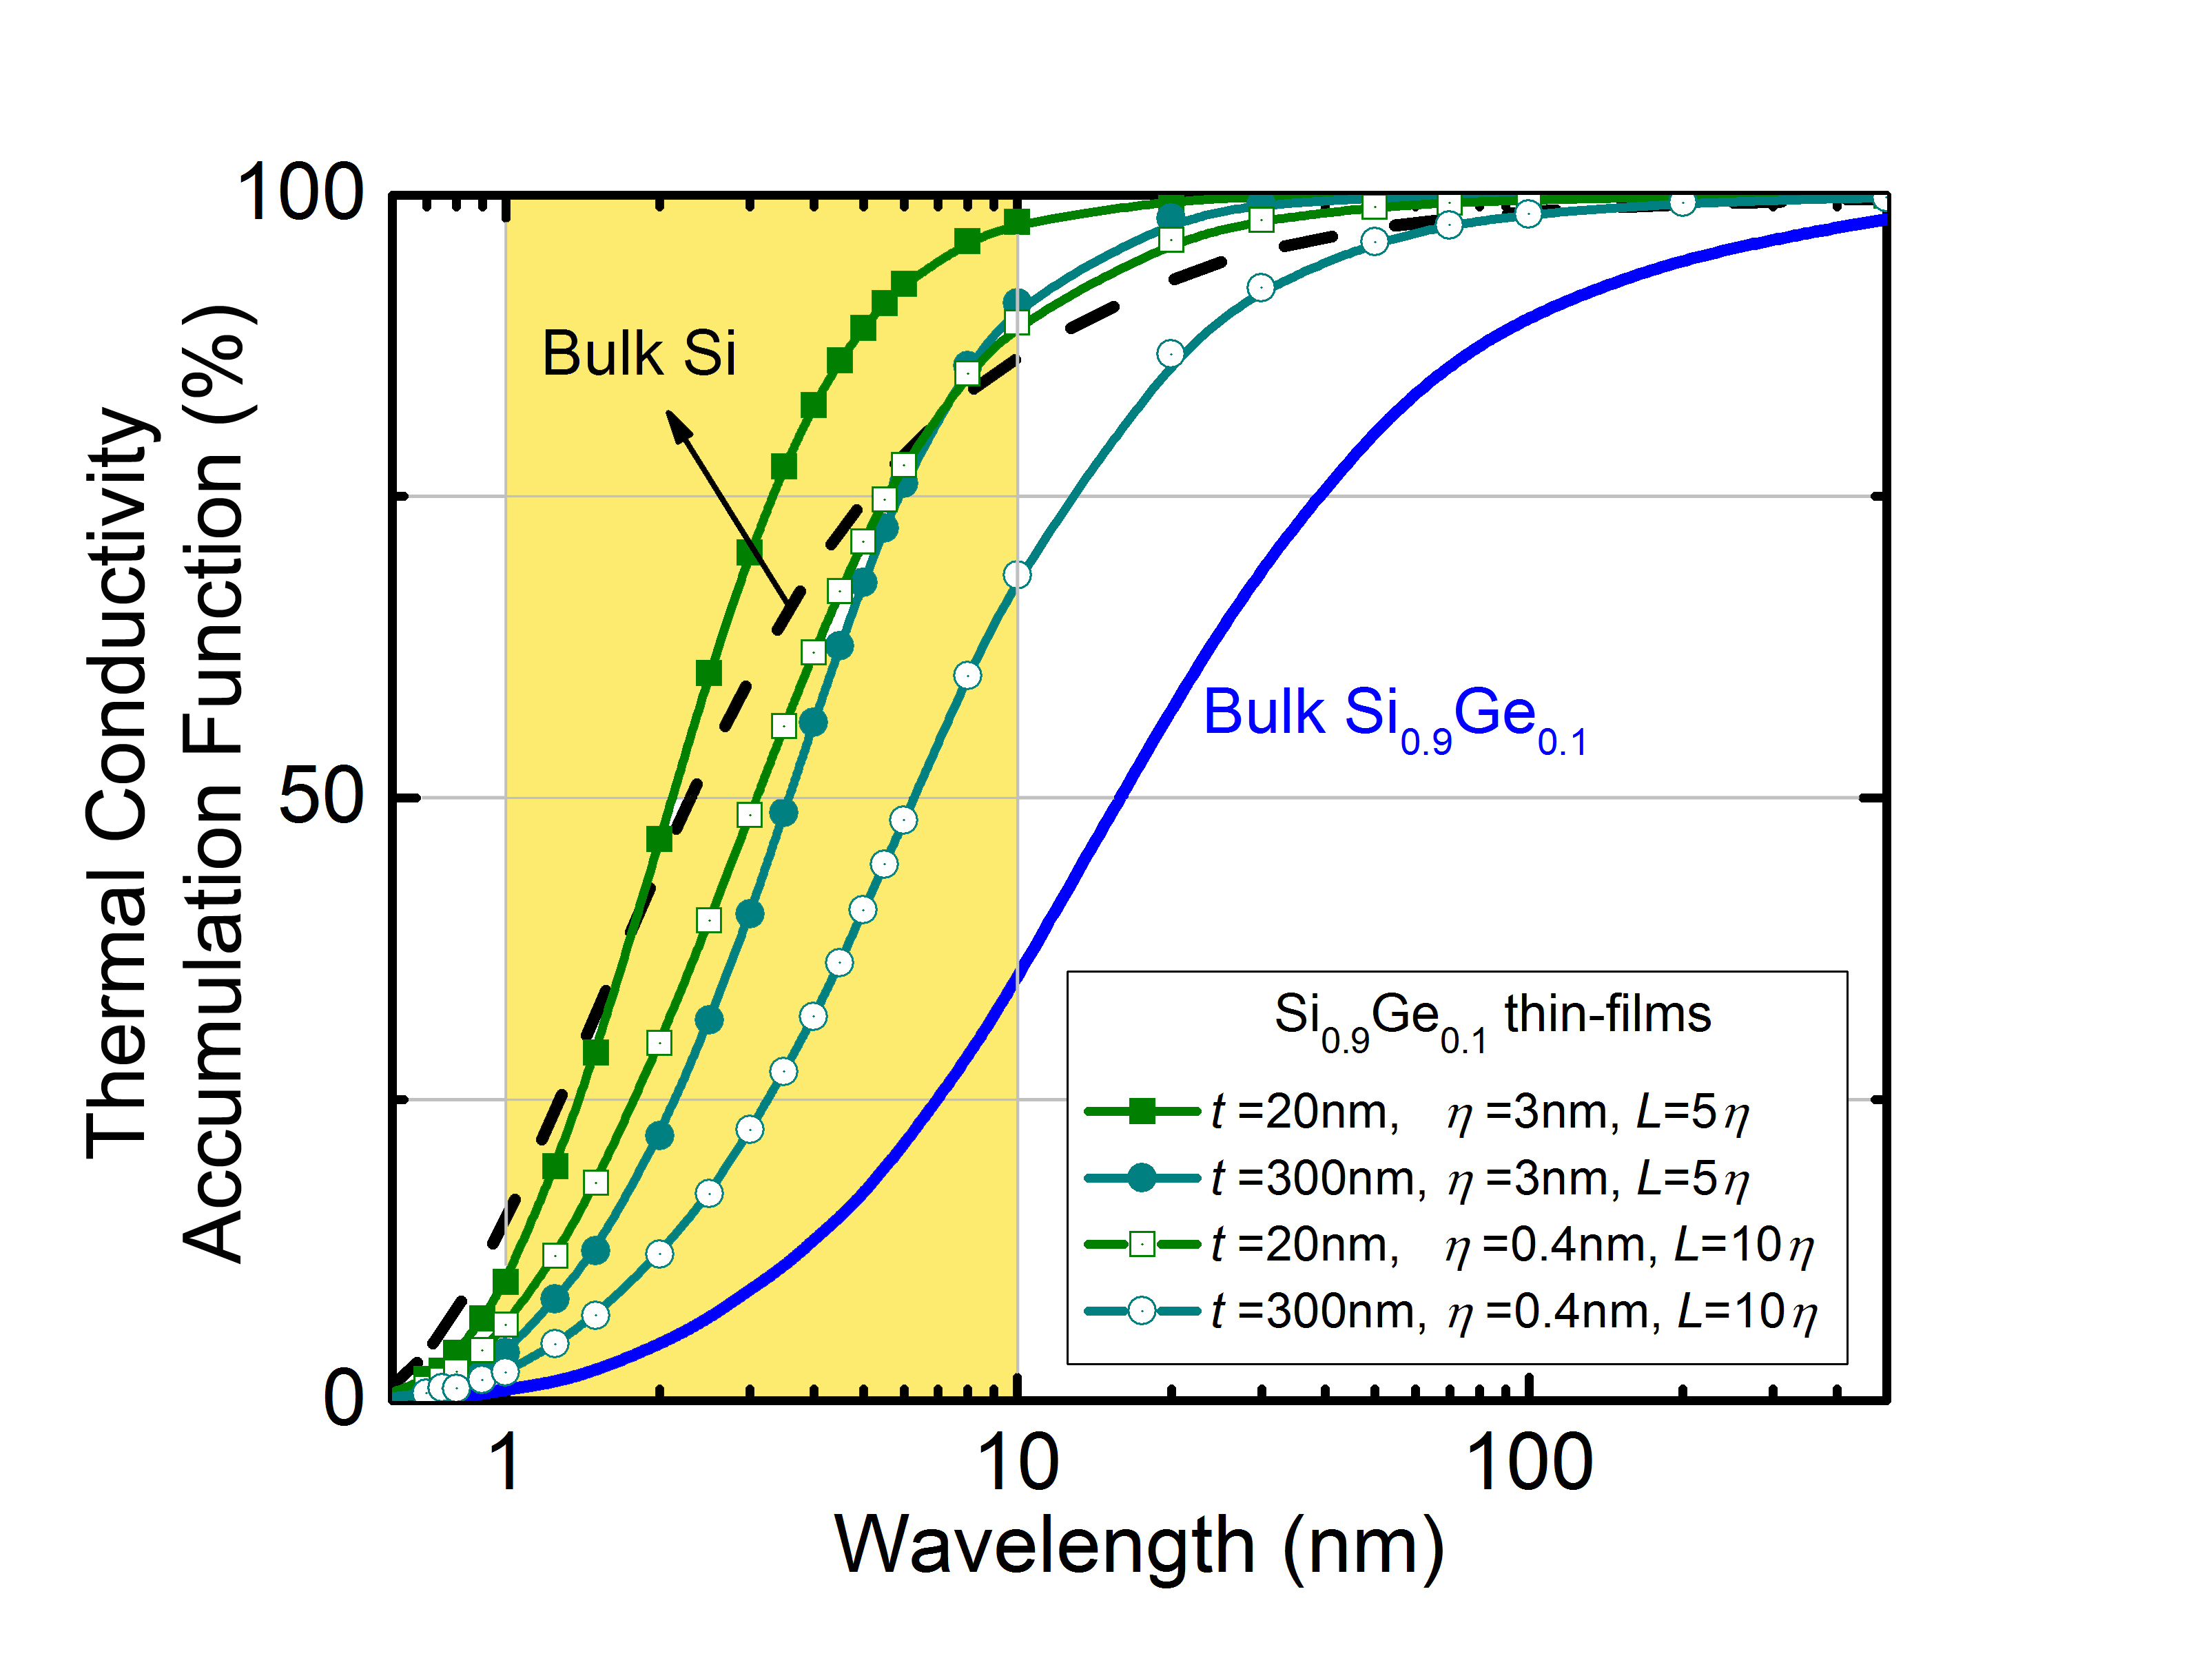
\includegraphics[width=\textwidth]{/ch2/Figure-TF-Spectra3.jpg}
  \caption{Thermal conductivity accumulation (or heat spectra) modification in \sige{0.90}{0.10} thin-films at room temperature by varying surface properties and thicknesses. Bulk Si and \sige{0.90}{0.10} accumulation functions are presented as reference. The proportion of heat carried by phonons with wavelengths \gls{wl} = 1–10 nm can be made to vary from 30\% to 90\% by tuning phonon scattering.}
  \label{fig:ch2-tf-spectra-3}
\end{figure}

\section{Estimating the Importance of Phonon Confinement}
It is important to highlight that advances in manufacturing techniques have enabled the production of thin films with very small thicknesses. At very small length scales, phonon quantum effects can become important and can play an important role in heat transport \cite{RN205,RN153}. Using our surface scattering and heat transport model, we show the emergence and impact of phonon quantum confinement effects \cite{RN139} in Si and SiGe thin-films. We note that a similar function can be defined for nanowires \cite{ownNW}. The introduction of the film boundaries allows for the creation of spatially confined phonons which behave as standing waves in the direction normal to the surfaces. We define a Confinement Contribution Fraction (CCF) to quantify the potential influence of phonon confinement in thin-films. CCF is calculated as the proportion of thermal energy conducted by phonons which can satisfy the confinement criteria in a nanostructure. Note that confined phonons may show modified transport properties, such as group velocities, due to coherent interference and resultant modified dispersion relations. Thus, a thin-film whose thermal conductivity values can be highly influenced by phonon quantum confinement exhibit a higher CCF value. The conditions that need to be satisfied by a phonon to be confined are twofold. First criterion requires mean-free-paths \gls{mfp} be sufficiently long so that phonons can effectively ``see" the two film boundaries. Second, Si-air interfaces (which behave as boundaries of infinite potential for the phonons) restrict and quantize the allowed wave vectors propagating in the direction normal to the surfaces when brought close together. Phonons with wavelengths larger than 2\gls{t} $\cos\theta$ (where \gls{t} is the thickness, and \gls{theta} the angle with surface normal) are entirely transformed to non-propagating modes, while larger k-space phonons can still propagate but subject to confinement effects \cite{book_Zangwill}. On the basis of this limiting condition, we define the minimum [i.e., $\lambda_1>2t\cos\theta$] and upper threshold [$\lambda_2>(2t\cos\theta)/5$] of the impact of confinement effects on heat conduction in Si and SiGe thin films and calculate the Confinement Contribution Fractions, CCF\textsubscript{min} and CCF\textsubscript{max}, respectively [\Cref{fig:ch2-confinement}(a) and (b)]. Note that the condition for $\lambda_2$ is an estimate to gauge the maximum influence of confinement in nanostructures based on the fact that the allowed wavelengths are discrete and quantized in a nanostructure. Specifically, the first five quantized values are separated to a larger degree than the subsequent values, and therefore, the middle-point of an order of magnitude change is taken as a measure of strong confinement effects (i.e., $\lambda_2$). Solid (CCF\textsubscript{min}) and dotted (CCF\textsubscript{max}) lines have similar values at large thicknesses because of the inability of the phonons to see the two interfaces due to phonon-phonon scattering. For intermediate thicknesses, the two lines separate as the wavelength conditions begin to dictate the possibility of confinement. At small thicknesses, even though a wide range of phonons can satisfy the wavelength confinement conditions, only a limited number of them with sufficiently large mean-free-paths (to form a standing wave) can show confinement. In general, rougher interfaces exhibit smaller confinement influenced conductivity as shown by smaller CCF values for \gls{eta} = 0.5 nm than \gls{eta} = 0.25 nm (\gls{cl} = 10\gls{eta} for both cases) and the contribution of phonon confinement effects reduces (marked by decreasing CCF) with increasing thicknesses. An analysis for temperature shows that confinement effects are significantly enhanced at lower temperatures as longer wavelength (and mean-free-path) phonons carry more heat. For example, in Si thin films of roughness 0.5 nm and \gls{cl} = 5 nm, CCF = 0.02 at room temperatures for 10 nm thick structures in contrast to CCF = 0.13 at 20 K. We note that for thicker (\gls{t}$\sim$30 nm) Si thin films at room temperatures, CCF values for typical interfacial roughness (\gls{eta} = 0.5 nm) quantitatively indicate that phonon confinement effects are negligible, while for very smooth interfaces (\gls{eta} = 0.25 nm) these effects are shown to be small. Similar trends with temperature are observed in the case of \sige{0.90}{0.10} alloyed thin films (CCF = 0.05 and 0.18 at 300 K and 20 K, respectively). Importantly, the use of only 10\% Ge makes the alloyed thin films a better candidate to explore confinement as compared to pure Si. This is due to the efficient scattering of small wavelengths by heavier atoms of Ge in the crystalline lattice of Si which shifts the thermal conductivity accumulation function towards larger wavelength thermal phonons as compared to crystalline Si.
\begin{figure}[hbt]
  \centering 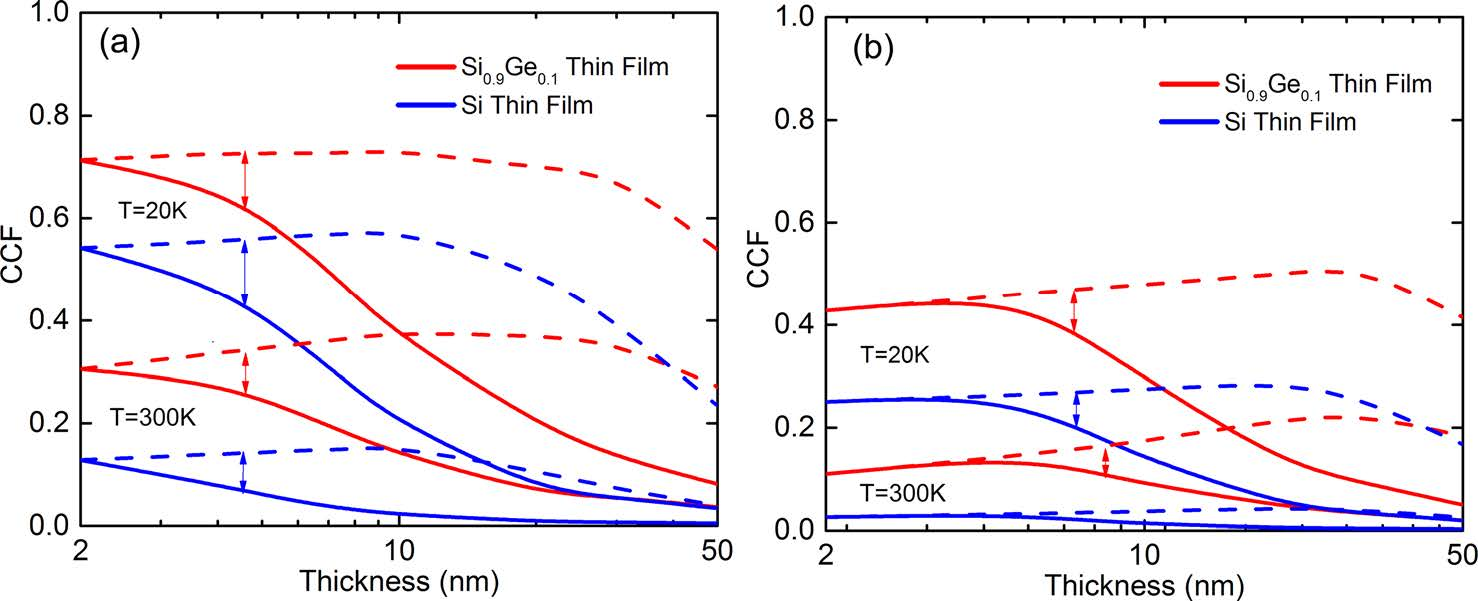
\includegraphics[width=\textwidth]{/ch2/Figure-TF-confinement.jpg}
  \caption{Confinement Contribution Functions (CCF) calculated at room temperature and \gls{T} = 20 K for thin films with correlation lengths \gls{cl} = 10\gls{eta} and roughness (a) \gls{eta} = 0.25 nm (b) \gls{eta} = 0.5 nm. CCF\textsubscript{min} (solid line) is the minimum contribution of confined modes to conductivity due to mode conversion in spatially confined nanostructures, while CCF\textsubscript{max} (dashed line) gives an upper threshold to this contribution. Double arrows are used as guide to the eyes.}
  \label{fig:ch2-confinement}
\end{figure}

\section{Summary}
The absence of rigorous theoretical descriptions for phonon-surface interaction have precluded the creation of truly predictive models which rely on experimentally quantifiable descriptors and embody key physics of phonon-surface scattering. To address this issue, we introduced an approach to predict heat transport in nanowires and thin films by considering the reduction in phonon mean-free-paths via the Beckmann-Kirchhoff rough surface scattering theory along with rough surface shadowing. This approach considers all critically relevant physical variables behind the phonon interface interactions and phonon transport viz. phonon momentum, angle of incidence of phonons with the surface, surface roughness and surface correlation length. We developed a model that could determine the energy distribution using the thermal conductivity accumulation function across phonon mean-free-paths and wavelengths in Si and SiGe nanowires and thin films with varying surface conditions. The applicability of our model is demonstrated by the excellent agreement with a range of experimental measurements. These results help to fundamentally understand heat transport at the nanoscale and provide a route to accurately establish the transport mechanisms with the use of experimentally quantifiable parameters.	

%%%%%%%%%%%%%%%%
% Chapter 3
%%%%%%%%%%%%%%%%

%!TEX root = thesis.tex
\chapter{Evolution of Thermal Flux in Asymmetric Thin-Films}
\label{chap:diff_boundary}
\section{Introduction}\blfootnote{Portions of this chapter have originally been published in \cite{ownSpatialTF} ``Spatial Manipulation of Thermal Flux in Nanoscale Films" (2017), \textit{Nanoscale and Microscale Thermophysical Engineering}, Vol. 21 (3), published by Taylor \& Francis.} 
 Although studies on the reduction in thermal conductivity of nanoscale thin films have attracted significant interest in recent years \cite{RN286,RN120,RN46,RN127,RN207,RN204,maldovan2011tf,RN189,RN208}, the spatial distribution of the heat flux and the possibility of modulating the flow of thermal energy within the nanostructure have received little attention. In this chapter, we study the effect of distinct surface properties on thermal transport in asymmetric thin-films. Previously in \Cref{chap:predictive}, we showed the development of thermal transport model for thin-films that assumed that the thin-film was symmetric, i.e. both the boundaries possessed identical surface features. Here, we extend the previous model to move beyond the symmetric nanostructure approximation and use the developed model to study the role of film thickness, alloying, and temperature on spatial distribution of thermal flux within thin films. We show that designing the physical properties of thin-film surfaces provides a control over the path taken by the thermal energy; for example, whether heat flows close to a surface or near the center of the film. We also show the strong dependence of these spatial flux profiles on the film thickness, temperature and alloying. The results presented in this work are valuable for the interpretation of theoretical and experimental measurements of thermal conductivities in semiconductor thin films, especially in the general case where the two surfaces of thin films may possess distinct surface specularities independent of one another, for which currently there are no theoretical models that can connect computations with measurements. Our findings help to advance the understanding of the nature of thermal fluxes within reduced geometries and provide an avenue for better integration of experimental and computational research efforts in the area of nanoscale thermal transport.
\section{Methodology}\label{sec:ch3-method}
The failure of Fourier’s laws at small length and timescales in nanoscale thin films marks a shift away from fully diffusive transport to a quasi-ballistic regime and necessitates the treatment of heat conduction via phonon transport. In the kinetic picture of quasi-ballistic transport, since the mean-free-paths of heat conducting phonons are longer than the thickness of the thin-films, it causes a change in their ability to conduct heat. In the phononic populations approach, this change in thermal properties can be understood as the deviation of phonon populations away from equilibrium. Here, we show \textit{two equivalent methodologies} that approach this transport physics in thin-films from the kinetic picture and phononic population perspective, respectively. 	
\subsection{System Description}
The system of interest is a thin-film [\Cref{fig:ch3-schematic}, top], of thickness \gls{t}. The surfaces of the thin-film are assumed to be independent of each other, thus have distinct surface properties in general. These distinct surface properties give rise to their individual specularity parameters, denoted as $p^{L}$ and $p^{U}$ for the lower and upper surface, respectively. Importantly, in both the formulations the surface specularity \gls{p} is not an arbitrary parameter but rather describes the physical interactions between phonons and thin-film boundaries and depends on the surface characteristics (roughness and correlation length) and phonon properties (incident angle on the surface and momentum), and physically represents the proportion of phonons that are specularly scattered upon interacting with the surface.

% schematic
\begin{figure}[hbt]
	\centering 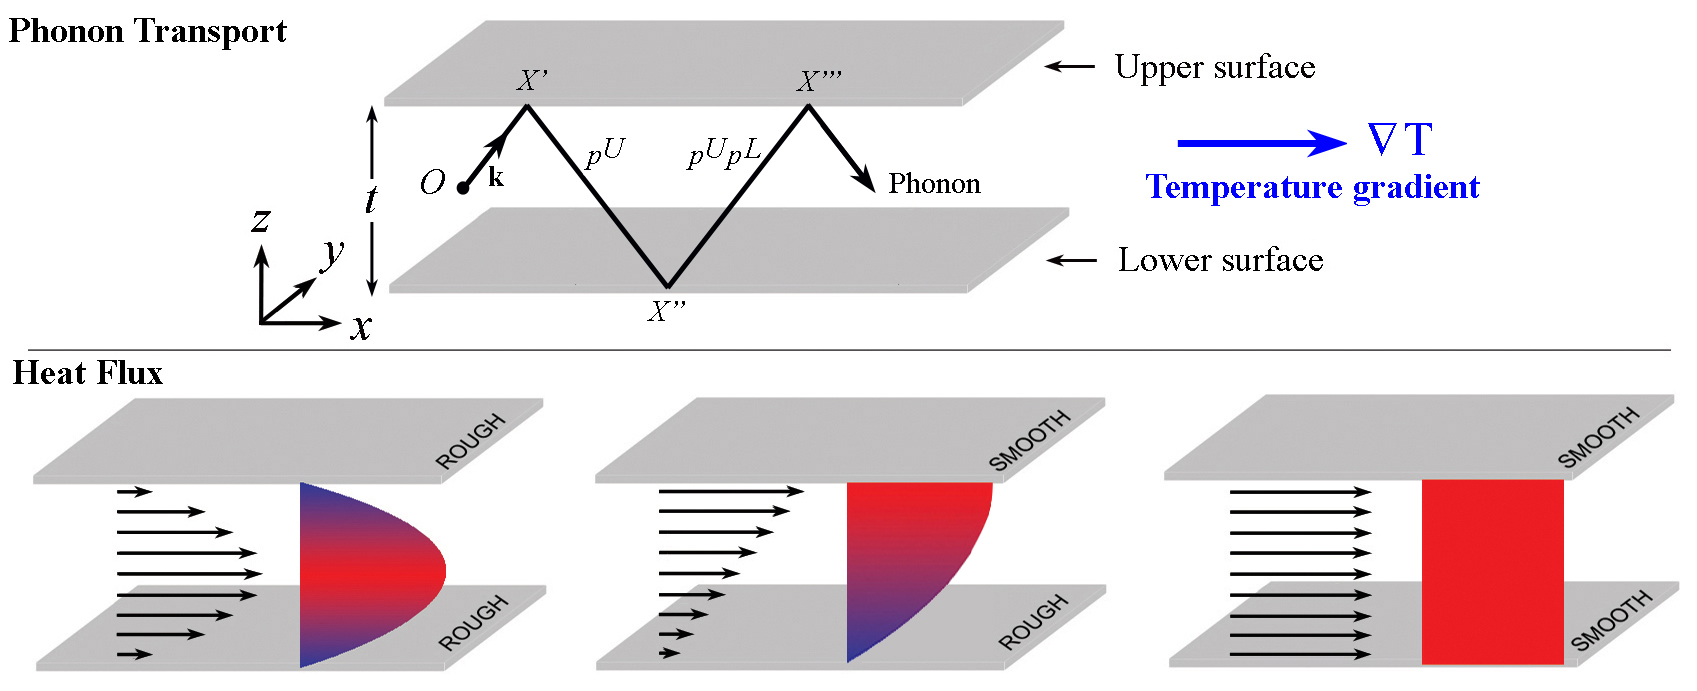
\includegraphics[width=\textwidth]{/ch3/Fig1.jpg}
	\caption{Top: Schematic representation of phonon transport in thin films where phonons originating at point O inside a thin film of thickness \gls{t} move under a thermal gradient \gls{gradT} along the in-plane direction. In the figure, the wavevector \gls{k} leads the phonon toward the upper surface possessing surface specularity $p^{U}$ and upon scattering is directed toward the lower surface possessing surface specularity $p^{L}$. Bottom: Schematic representation of heat flux spatial distribution within thin films depending on the surface conditions (smooth or rough) of the boundaries.}
	\label{fig:ch3-schematic}
\end{figure}

\subsection{Reduced Mean-Free-Path Approach}
Similar to the derivation shown in \Cref{sec:MFPRedModel}, we evaluate the changes in phononic mean-free-paths \gls{mfp}. Here, however, since the two surfaces are distinct, the model needs to differentiate among phonons originating with positive and negative wave vectors along the z-coordinate [\Cref{fig:ch3-schematic}, top]. For example, phonons with positive $\mathbf{k}_{z}$ will see first the upper surface at $z = t$ and will thus be first scattered at point $X^{'}$ accompanied by change in sign of $\vec{k}_{z}$. At every interaction with the upper surface, a proportion of phonons, $1-p^{U}$ are scattered diffusively. Similarly, phonons with initial negative $\mathbf{k}_{z}$ interact with lower surface at $z=0$ first where $1-p^{L}$ proportion of incident phonons are scattered diffusively. By writing $OX^{'}=\Lambda$, the contribution to the mean-free-path for phonons up to the point $X^{'}$ is evaluated to be,

\begin{equation}
\ell_{\vec{k}}^{{OX^{'}}}=\int_{0}^{\Lambda}{\frac{r}{\ell_{\vec{k}}^{\textrm{bulk}}}\exp\Big({-\frac{r}{\ell_{\vec{k}}^{\textrm{bulk}}}} \Big)\,dr} + (1-p^{U})\int_{\Lambda}^{\infty} {\frac{\Lambda}{\ell_{\vec{k}}^{\textrm{bulk}}}\exp\Big({-\frac{r}{\ell_{\vec{k}}^{\textrm{bulk}}}}\Big)\,dr}
\label{eq:ox}
\end{equation} 
For phonons subsequently specularly reflected and moving between $X^{'}$ and $X^{''}$, the contribution to the mean-free-path can analogously be written as,
\begin{equation}
\ell_{\vec{k}}^{{X^{'}X^{''}}}=p^{U}\int_{\Lambda}^{\Lambda+\Lambda^{*}}{\frac{r}{\ell_{\vec{k}}^{\textrm{bulk}}}\exp\Big({-\frac{r}{\ell_{\vec{k}}^{\textrm{bulk}}}} \Big)\,dr} + p^{U}(1-p^{L})\int_{\Lambda+\Lambda^{*}}^{\infty} {\frac{\Lambda+\Lambda^{*}}{\ell_{\vec{k}}^{\textrm{bulk}}}\exp\Big({-\frac{r}{\ell_{\vec{k}}^{\textrm{bulk}}}}\Big)\,dr}
\label{eq:xx}
\end{equation} 
Note that the first term in \Cref{eq:xx} represents the contribution of the fraction $p^{U}$ of phonons that are specularly reflected at $X^{'}$ and the second term represents the contribution of the fraction $p^{U} (1-p^{L})$ of phonons that are diffusively scattered upon interacting with the surface at $X^{''}$. The total reduced mean-free-path can be obtained by summing the contributions from terms in \Cref{eq:ox,eq:xx} and the successive terms expanded similarly, which yields the general form of the reduced mean-free-path for a thin film with arbitrary, distinct surface specularities at the film boundaries as:

\begin{equation}
\ell_{\vec{k}}(z)= 
\begin{cases}
\ell_{\vec{k}}^{\textrm{bulk}}\Bigg(\dfrac{1-\Theta_1 + p^L p^U \Theta_2 \Theta_3 - (1-p^U + p^U \Theta_2 ) \Theta_3 }{1-\Theta_1}\Bigg) & \text{if}\: \vec{k}_z >0 \\
\ell_{\vec{k}}^{\textrm{bulk}}\Bigg(\dfrac{1-\Theta_1 + p^L p^U \Theta_2 \Theta_3 - (1-p^L + p^L \Theta_2 ) \Theta_3 }{1-\Theta_1}\Bigg) & \text{if}\: \vec{k}_z <0	
\end{cases}
\label{eq:mfp_ch3}
\end{equation} 
where,
\begin{align}\label{eq:mfp_params_ch3}
	\Theta_1 &= p^L p^U \exp (-2\Lambda^*/\ell_{\vec{k}}^{\textrm{bulk}}) \nonumber \\
	\Theta_2 &= \exp (-\Lambda^*/\ell_{\vec{k}}^{\textrm{bulk}}) \\
	\Theta_3 &= \exp (-\Lambda/\ell_{\vec{k}}^{\textrm{bulk}}) \nonumber
\end{align}

Thus, \Cref{eq:mfp_ch3,eq:mfp_params_ch3} are used to obtain the reduced phonon mean-free-paths which depend on the spatial position within the thin-film. Thus, the thermal flux obtained using these mean-free-paths is dependent on the spatial position as indicated by the integrand of the spatial domain in \Cref{eq:phonon_fourier}. 

\subsection{Non-equilibrium Population Distribution Approach}
The local population of phonons \gls{f}$(r)$ in a thin-film under an in-plane gradient is deviated from equilibrium Bose-Einstein distribution \gls{fBE}. For a steady state BTE (see \Cref{eq:bte_ss}) applied to a thin-film, the solution to non-equilibrium phonon populations can be written as \cite{book_Ziman}:

\begin{equation}\label{eq:ch3-5}
  f_\vec{k}=  f_\vec{k}^{BE}-\tau_\vec{k}\frac{\partial f_\vec{k}^{BE}}{\partial T}\Bigg(1+\Phi_\vec{k}\exp\Big(-\dfrac{z}{\tau_\vec{k} v_\vec{k}}\Big)\Bigg)v_\vec{k}\cdot \nabla T 
\end{equation}
where $\Phi_\vec{k}$ is determined by the boundary conditions of the thin-film. As a result, a closed-form solution of the BTE in terms of local phonon populations or equivalently, in terms of a deviation function $g_\vec{k} = f_\vec{k} - f_\vec{k}^{BE}$ of phonon populations from equilibrium, can be obtained by imposing the boundary conditions for the thin-film geometry. The boundary conditions can be written following a balance of phonon populations incoming and outgoing from the surfaces. The phononic deviation functions are divided into two components, $g_\vec{k}^+$ and $g_\vec{k}^-$ denoting the populations with positive and negative z-components of \gls{k}.
\begin{align}\label{eq:boundary_conditions_ch3_1}
	[f^{BE}+g_\vec{k}^+(z=0)] &= p^L [f^{BE}+g_\vec{k}^-(z=0)]+[1-p^L]f^{BE} \\
	[f^{BE}+g_\vec{k}^-(z=t)] &= p^U [f^{BE}+g_\vec{k}^+(z=t)]+[1-p^U]f^{BE}
\label{eq:boundary_conditions_ch3_2}
\end{align}

Using \Cref{eq:boundary_conditions_ch3_1,eq:boundary_conditions_ch3_2}, the deviation from equilibrium can be calculated to be,
\begin{equation}\label{eq:ch3_g}
g_\vec{k}(z)=
\begin{cases} 
-\tau_\vec{k}v_{\vec{k}|x}\frac{\partial f_\vec{k}^{BE}}{\partial T}\frac{\partial T}{\partial x}\Big[1-\frac{1-p^L+p^L(1-p^U)\exp(-t/\tau_\vec{k}v_{\vec{k}|z})}{1-p^Lp^U\exp(-2t/\tau_\vec{k}v_{\vec{k}|z})}\exp\Big(-\dfrac{z}{\tau_\vec{k}v_{\vec{k}|z}}\Big) \Big] & \: \vec{k}_z >0 \\
-\tau_\vec{k}v_{\vec{k}|x}\frac{\partial f_\vec{k}^{BE}}{\partial T}\frac{\partial T}{\partial x}\Big[1-\frac{1-p^U+p^U(1-p^L)\exp(t/\tau_\vec{k}v_{\vec{k}|z})}{1-p^Lp^U\exp(2t/\tau_\vec{k}v_{\vec{k}|z})}\exp\Big(-\dfrac{z-t}{\tau_\vec{k}v_{\vec{k}|z}}\Big) \Big] & \: \vec{k}_z <0
% & \: \vec{k}_z <0	
\end{cases}
\end{equation}
where the $x$ and $z$ in the subscripts represent the components along those Cartesian directions. 
\subsection{Equivalence of Approaches}
In order to establish the fundamental equivalence of the two mathematical interpretations of behavior of phonons i.e. the kinetic approach to model modified phononic mean-free-paths and the deviation of phononic populations from equilibrium, we calculate the spatially averaged thermal conductivity from the two approaches using \Cref{eq:phonon_fourier} and \Cref{eq:pop_fourier}, respectively. We create test cases covering a range of conditions under varying roughness, correlation lengths, temperature and thin-film thickness which are detailed in \Cref{tab:parameters-validation}. 
\\
% This is a table
\begin{table}[hbt]
\centering
\caption{Test cases to examine the equivalence between reduced mean-free-path approach and deviation of population from equilibrium approach.}
\resizebox{\linewidth}{!}{%
\begin{tabular}{lcccccc} 
\toprule[\heavyrulewidth]\toprule[\heavyrulewidth]
Case \# & Thickness~(nm) & \begin{tabular}[c]{@{}l@{}}Upper Surface \\Roughness (nm)\end{tabular} & \begin{tabular}[c]{@{}l@{}}Lower Surface \\Roughness (nm)\end{tabular} & $\mathcal{L}^U/\eta^U$ & $\mathcal{L}^L/\eta^L$ & Temperature (K)  \\ 
\hline
A       & 30             & 0.5                                                                    & 0.5                                                                    & 8              & 10             & 300             \\
B       & 50             & 0.1                                                                    & 0.5                                                                    & 10             & 8              & 50              \\
C       & 100            & 0.5                                                                    & 0.5                                                                    & 10             & 10             & 300             \\
D       & 200            & 0.01                                                                   & 1.0                                                                    & 20             & 6              & 800             \\
E       & 500            & 0.25                                                                   & 1.5                                                                    & 15             & 8              & 300             \\
F       & 2000           & 0.5                                                                    & 0.5                                                                    & 10             & 10             & 300             \\
\bottomrule[\heavyrulewidth]
\end{tabular}
}
\label{tab:parameters-validation}
\end{table}

Average conductivity is evaluated using the gradient along with the integral of local flux distributions over the thickness of the film. The comparison of the conductivities is presented in \Cref{fig:ch3-validation}, from which it is evident that the two approaches generate nearly identical values of thermal conductivities for different values of thickness and surface properties which establishes the equivalency between the methods. The adjusted R-square of the linear fit between calculated values from the two approaches for the six cases is \textgreater 0.999, establishing the equivalence. Since the two approaches are mathematically equivalent, further analysis can be conducted by proceeding with any of the two methods without any loss of generality. In \Cref{sec:results_ch3}, we choose to use the reduced mean-free-path approach to calculate transport properties for two major reasons. Firstly, reduced mean-free-path approach preserves the mean-free-paths of phonons explicitly which are an important physical quantity especially for rational design of materials and in understanding behavior of phonons and heat at nanoscale. Secondly, a higher computational efficiency is achieved in the numerical integration routine in reduced mean-free-path approach reducing the cost of implementation.
% schematic
\begin{figure}[hbt]
	\centering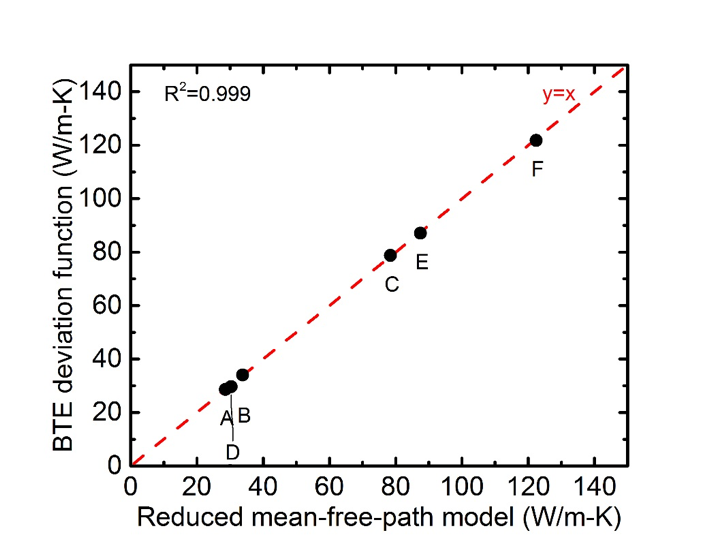
\includegraphics[width=0.75\textwidth]{/ch3/Fig2.png}
	\caption{Comparison between averaged thermal conductivity obtained from reduced mean-free-path model ($x$-axis) and deviation function via a semi-analytical BTE solution ($y$-axis), showing the equivalence of the two approaches}
	\label{fig:ch3-validation}
\end{figure}

\subsection{Note on Surface Specularity}
To obtain the surface specularity at the distinct thin-film boundaries, we utilize our previously developed (see \Cref{sec:BK}) BK surface scattering model extended with surface shadowing effects on heat conduction. The surface specularity \gls{p} obtained from the BK and shadowing theory contains a description of phonon–surface scattering that accounts for its dependence on all relevant physical variables -- phonon properties (momentum and incident angle \gls{thetai} via the wave-vector \gls{k}) and surface characteristics (roughness \gls{eta} and correlation length \gls{cl}); that is, $p = p(k, \theta_i, \eta, \mathcal{L})$.

\section{Results and Discussion}\label{sec:results_ch3}
Using our approach, we move beyond simplifying assumptions about phonon-surface scattering (e.g., constant specularity or complete diffuse scattering) in thin films and connect the physical properties of general surfaces with the spatial distribution of the thermal flux within the thin films. We note that the analogy between transport of momentum, heat, and mass has been central in many fields of engineering \cite{book_Bird}. For continuum fluids, the “no-slip” condition at a solid-fluid interface generates fluid flux spatial distributions in a number of interesting fluid phenomena, including the dynamics of falling films, flow in confined geometries, and boundary layers. Interestingly, such no-slip behavior of momentum-flux has no classical analogue in thermal transport at the continuum bulk scale. However, the existence of spatial boundaries in thin films creates a thermal flux that is a function of the spatial location within the film, analogous to fluid dynamics. 

Before analyzing the effects of surface conditions on local heat flux distributions, we apply our methodology to a particular case of a thin film of thickness \gls{t} = 100 nm at room temperature under a temperature gradient (1 K/\si{\micro}m) with equal surface properties on the two very rough boundaries (i.e., complete diffusive scattering). \Cref{fig:ch3-comparison} shows the effect of phonon–surface interactions on the local heat flux and quantitatively shows that heat conduction in a thin film with completely diffusive boundaries can be considered analogous to no-slip fluid flow in a rectangular pipe with fixed walls in the sense that the thermal flux reaches a maximum at the center. However, a clear distinction between momentum and heat transport in the form of a nonzero local value of heat flux near diffusive domain boundaries should be noted. The physical mechanism behind this spatial dependence of thermal flux distribution is the momentum randomization of diffusively scattered phonons at the surfaces, which reduces the phonon mean-free-paths depending on the distance between the surface and the point where the phonon originates [\Cref{fig:ch3-schematic}]. The agreement in the values of normalized flux for the particular case of identical diffusive surfaces \cite{RN445,RN276} serves as validation of the reduced mean-free-path methodology. Our proposed model, however, allows us to consider more general and realistic surface conditions, including different surface roughnesses and correlation lengths, as well as independent surface conditions on the two boundaries of the films.
%figure
\begin{figure}[hbt]
	\centering\includegraphics[width=0.95\textwidth]{/ch3/Fig3.jpg}
	\caption{Comparison of normalized heat flux in a 100nm Si thin film with fully diffusive upper and lower surfaces calculated by the reduced mean-free-path model (this work), Monte Carlo simulations \cite{RN445}, and variance-reduced Monte Carlo calculation \cite{RN276}. A maximum flux value is used for normalization.}
	\label{fig:ch3-comparison}
\end{figure}

Next, we use the flexibility of our reduced mean-free-path approach in terms of being able to treat general surface properties and study thermal transport properties and spatial distributions of thermal energy in thin films with surfaces possessing different roughnesses. We first analyze the effect of surface conditions on thermal flux distribution in a silicon thin film. We introduce a spatial asymmetry in the nanostructure by changing the surface properties of the boundaries of the thin film. Specifically, the roughness \gls{eta} (and correlation length \gls{cl}) for the upper surface is fixed to be $\eta^U$ = 4 nm ($\mathcal{L}^U = 10\eta^U$), and the surface properties of the lower surface are varied by changing the surface roughness to be $\eta^L$ = 0.25, 0.50, and 4.0 nm and maintaining the correlation length-to-roughness ratio ($\mathcal{L}^L = 10\eta^L$). In \Cref{fig:ch3-results-flux}, we show the existence of a thermal transport regime where heat conduction is spatially asymmetric, and the root of such a phenomenon lies in the differential behavior of the surface boundaries. As seen in the central panel of \Cref{fig:ch3-results-flux}, in a silicon film of thickness \gls{t} = 100 nm at room temperature, a roughness reduction at the lower surface (and corresponding correlation length) compared to the upper surface is accompanied by an increased asymmetry in the thermal flux, with more heat current flowing through the lower half of the film, as indicated by the increasing difference between the values of the thermal flux at the two boundaries. Additionally, the locus of peak flux shifts toward the lower surface as the difference in the roughness between the two boundaries is increased; that is, a larger proportion of thermal energy flows through the lower half of the thin film. Another key aspect of the flux profiles is the forward shift in the overall heat flux values corresponding to a net higher conduction in films with smoother surfaces. These results quantitatively show how an asymmetry in the surface properties of the two thin-film boundaries creates an asymmetry in the thermal flux within a thin film. \Cref{fig:ch3-results-flux}(a-c) show that the impact of distinct surface conditions on flux distributions is maintained across different thicknesses \gls{t} = 10, 100, 1000 nm. Note that the magnitude of flux increases overall with increasing thickness because the thermal transport at these length scales is quasi-ballistic and dependent on the size of the nanostructure. Importantly, the shape of the spatial flux diagram shows that, at an increased thickness [\Cref{fig:ch3-results-flux}(c)], the difference between the flux conducted near the edges of the thin film and at the center significantly increases. We also show in \Cref{fig:ch3-results-flux}(b,d,e) the impact of changes in temperature on the spatial distribution of thermal flux. A stronger role of the interfaces at lower temperatures is observed in the effective thermal flux due to the larger bulk phonon mean-free-paths. The changed magnitude of flux with temperature is also a consequence of modified internal scattering rates, with reduced phonon-phonon scattering rates occurring at lower temperatures. For the range of temperatures considered (\gls{T} = 100, 300, 700 K), the effects on the internal spatial distribution of the thermal energy is less pronounced than those arising from a change in the thickness of the film. Importantly, we have shown that heat flow can be manipulated to move closer to the center or near a surface of the film by purposely modifying the surface properties.
\par The observed behavior showing larger heat flux near smoother interfaces leads us to postulate that whereas a very rough diffuse boundary is analogous to fixed walls in fluid flow, a surface with small roughness (and in the limiting case of unity specularity) would be analogous to a plug fluid flow regime \cite{book_Bird}. We note that a surface boundary with specularity \gls{p} = 1 requires perfectly smooth thin-film boundaries devoid of any surface perturbations, which are difficult to create in experimentally grown Si nanostructures \cite{RN274,RN337}. \Cref{fig:ch3-results-flux-fluid}(a) shows normalized thermal flux profiles in thin films with limiting theoretical surface specularity values \gls{p} = 0 (completely diffuse) and \gls{p} = 1 (completely specular) for all phonons irrespective of their wavelength or incident angle. It is clearly seen that the heat flux near a diffusive boundary is suppressed, whereas phonon conduction near a specular boundary is less affected. Interestingly, when both surface boundaries are entirely specular, a constant thermal flux profile is obtained, analogous to a ``perfect plug flow" fluid velocity profile in a closed conduit. In this specular case, there is no randomization of phonon momentum upon encountering the surface, and the thermal flux is transported uninhibited. Such a constant thermal flux profile is also expected in bulk crystals. A nearly perfect plug flow is found in films with thicknesses in which the effects of the boundaries and interfacial phonon dynamics are negligible, as shown in the heat flux distribution calculated for a film of \gls{t} = 100 \si{\micro}m at room temperature [\Cref{fig:ch3-results-flux-fluid}(b)]. Most of the volume in a 100 \si{\micro}m silicon film is far away from the influence of the boundaries and exhibits a nearly constant, surface-independent flux similar to a perfect plug flow regime. Still the phonons close to the surfaces still interact with the boundaries (despite the overall dominating effect of internal phonon scattering processes in thicker films), creating their reduced mean-free-paths. %figure
\clearpage
\begin{sidewaysfigure}[hbt]
	\centering\includegraphics[width=1\textwidth]{/ch3/Fig4.jpg}
	\caption{Thermal flux profiles in Si thin films under a temperature gradient of 1\si{\kelvin\per\micro\meter} are shown as a function of temperature (\gls{T} = 100, 300, and 700 K) and thicknesses (\gls{t} = 10 nm, 100 nm, and 1 \si{\micro}m). Moving left to right, the thickness increases (upper panels) and the temperature decreases (lower panels). The central panel (b) shows the flux profiles at \gls{T} = 300 K and thickness \gls{t} = 100 nm. The surface roughness of the upper boundary is \gls{eta} = 4 nm and the roughness of the lower boundary is varied as \gls{eta} = 4 nm (blue), 0.5 nm (green), and 0.25 nm (red lines). The correlation length \gls{cl} is 10 times the roughness at both the surfaces.}
	\label{fig:ch3-results-flux}
\end{sidewaysfigure}
\clearpage
%figure
\begin{figure}[hbt]
	\centering\includegraphics[width=1\textwidth]{/ch3/Fig5.jpg}
	\caption{(a) Normalized thermal flux profiles in an Si thin film with varying surface conditions (limiting cases \gls{p} = 0 and \gls{p} = 1) are shown for a film thickness of \gls{t} = 100 nm at room temperature. (b) Nearly ideal plug flow profile development in very thick films where variations in thermal flux spatial distribution is constrained around the boundaries.}
	\label{fig:ch3-results-flux-fluid}
\end{figure}

Thus, the thermal flux deviates significantly from the bulk value only at spatial locations in the vicinity of the thin-film boundaries. However, because this deviation occurs in a very small spatial domain (compared to the overall thickness of the film), the averaged thermal conductivity is nearly unaffected by the deviations from plug flow flux profile in such large thickness films.
\section{Summary}
In this chapter, we analyzed the most general case of thin films; i.e., films with boundaries possessing independent surface properties. To study heat conduction processes in such thin-films, we developed two approaches. The first approach is based on determining the reduced phonon mean-free-path while the second approach is based on solving BTE to obtain non-equilibrium phonon populations. After establishing their equivalence, the former approach was utilized to evaluate thermal fluxes. We found that heat flux can be engineered to flow close to a surface or near the center of the film. We also showed the existence of heat transport regimes resembling fluid flow in confined geometries. The development of asymmetry in thermal flux with increasing difference between interface roughness properties were established. The results in this chapter show that computational tools with accurate boundary scattering mechanisms can yield insights about thermal transport phenomena and underscore the importance of interfacial phonon dynamics in heat conduction pathways in nanostructures. Furthermore, the methods described here move beyond the commonly used diffuse scattering surface assumptions, enabling the surfaces of nanostructures to be precisely described, strengthening the predictive power of models.


%%%%%%%%%%%%%%%%
% Chapter 4
%%%%%%%%%%%%%%%%

%!TEX root = thesis.tex
\chapter{Thermal Transport in Nanotubes }
\label{chap:nt}
\section{Introduction}\blfootnote{Portions of this chapter have originally been published in \cite{ownNT} ``Thermal Transport in Semiconductor Nanotubes" (2019), \textit{International Journal of Heat and Mass Transfer}, Vol. 130 (368), Elsevier Publishing.}
One-dimensional nanostructures such as nanowires, nanotubes, and nanofibers have exhibited potential in the development of more efficient thermoelectrics \cite{NW_hochbaum}, electronics \cite{RN502,RN425}, optoelectronics \cite{RN421,RN420}, and catalysts \cite{RN424,RN426}. The continuing advances in both top-down and bottom-up growth of semiconductor nanostructures have enabled the creation of novel 1-D morphologies which include nanotubes (or tubular nanowires) \cite{RN427,RN429}, core-shell heterostructures \cite{RN452,RN141,RN432}, and wires with different cross-sectional geometries \cite{RN145,RN483}. Here we focus on tubular nanowires or nanotubes, which have been experimentally studied recently and have been identified as potential energy materials \cite{RN456,RN436}. 

As we noted in previous chapters, the change in thermal transport properties in nanoscale semiconductors from their bulk values stems from the modifications in the transport dynamics of phonons. Despite their vast potential in thermal applications, a precise understanding of phonon transport in semiconductor nanotubes and the role of interfacial properties has remained limited. Early numerical and analytical attempts to model thermal transport in nanotubes had relied on the simplified assumption of frequency-independent phonon mean-free-paths (i.e. ‘gray approximation’) \cite{RN431}. Atomistic simulations while accounting for the broadband nature of phonon transport, have remained limited to very small structural sizes owing to their high computational requirements \cite{RN432}. The treatment of boundaries without considering experimentally quantifiable surface properties such as surface roughness or correlation lengths limits the insights provided by thermal transport models. In addition, the use of frequency-independent specularities for phonon-boundary interactions and the Matthiessen’s rule to combine phonon-boundary and phonon-phonon interactions into an effective phonon mean-free-path have also prevented the accurate description of phonon dynamics in nanotubes \cite{RN437}.

\section{Model}
% Schematic
\begin{figure}[hb]
	\centering 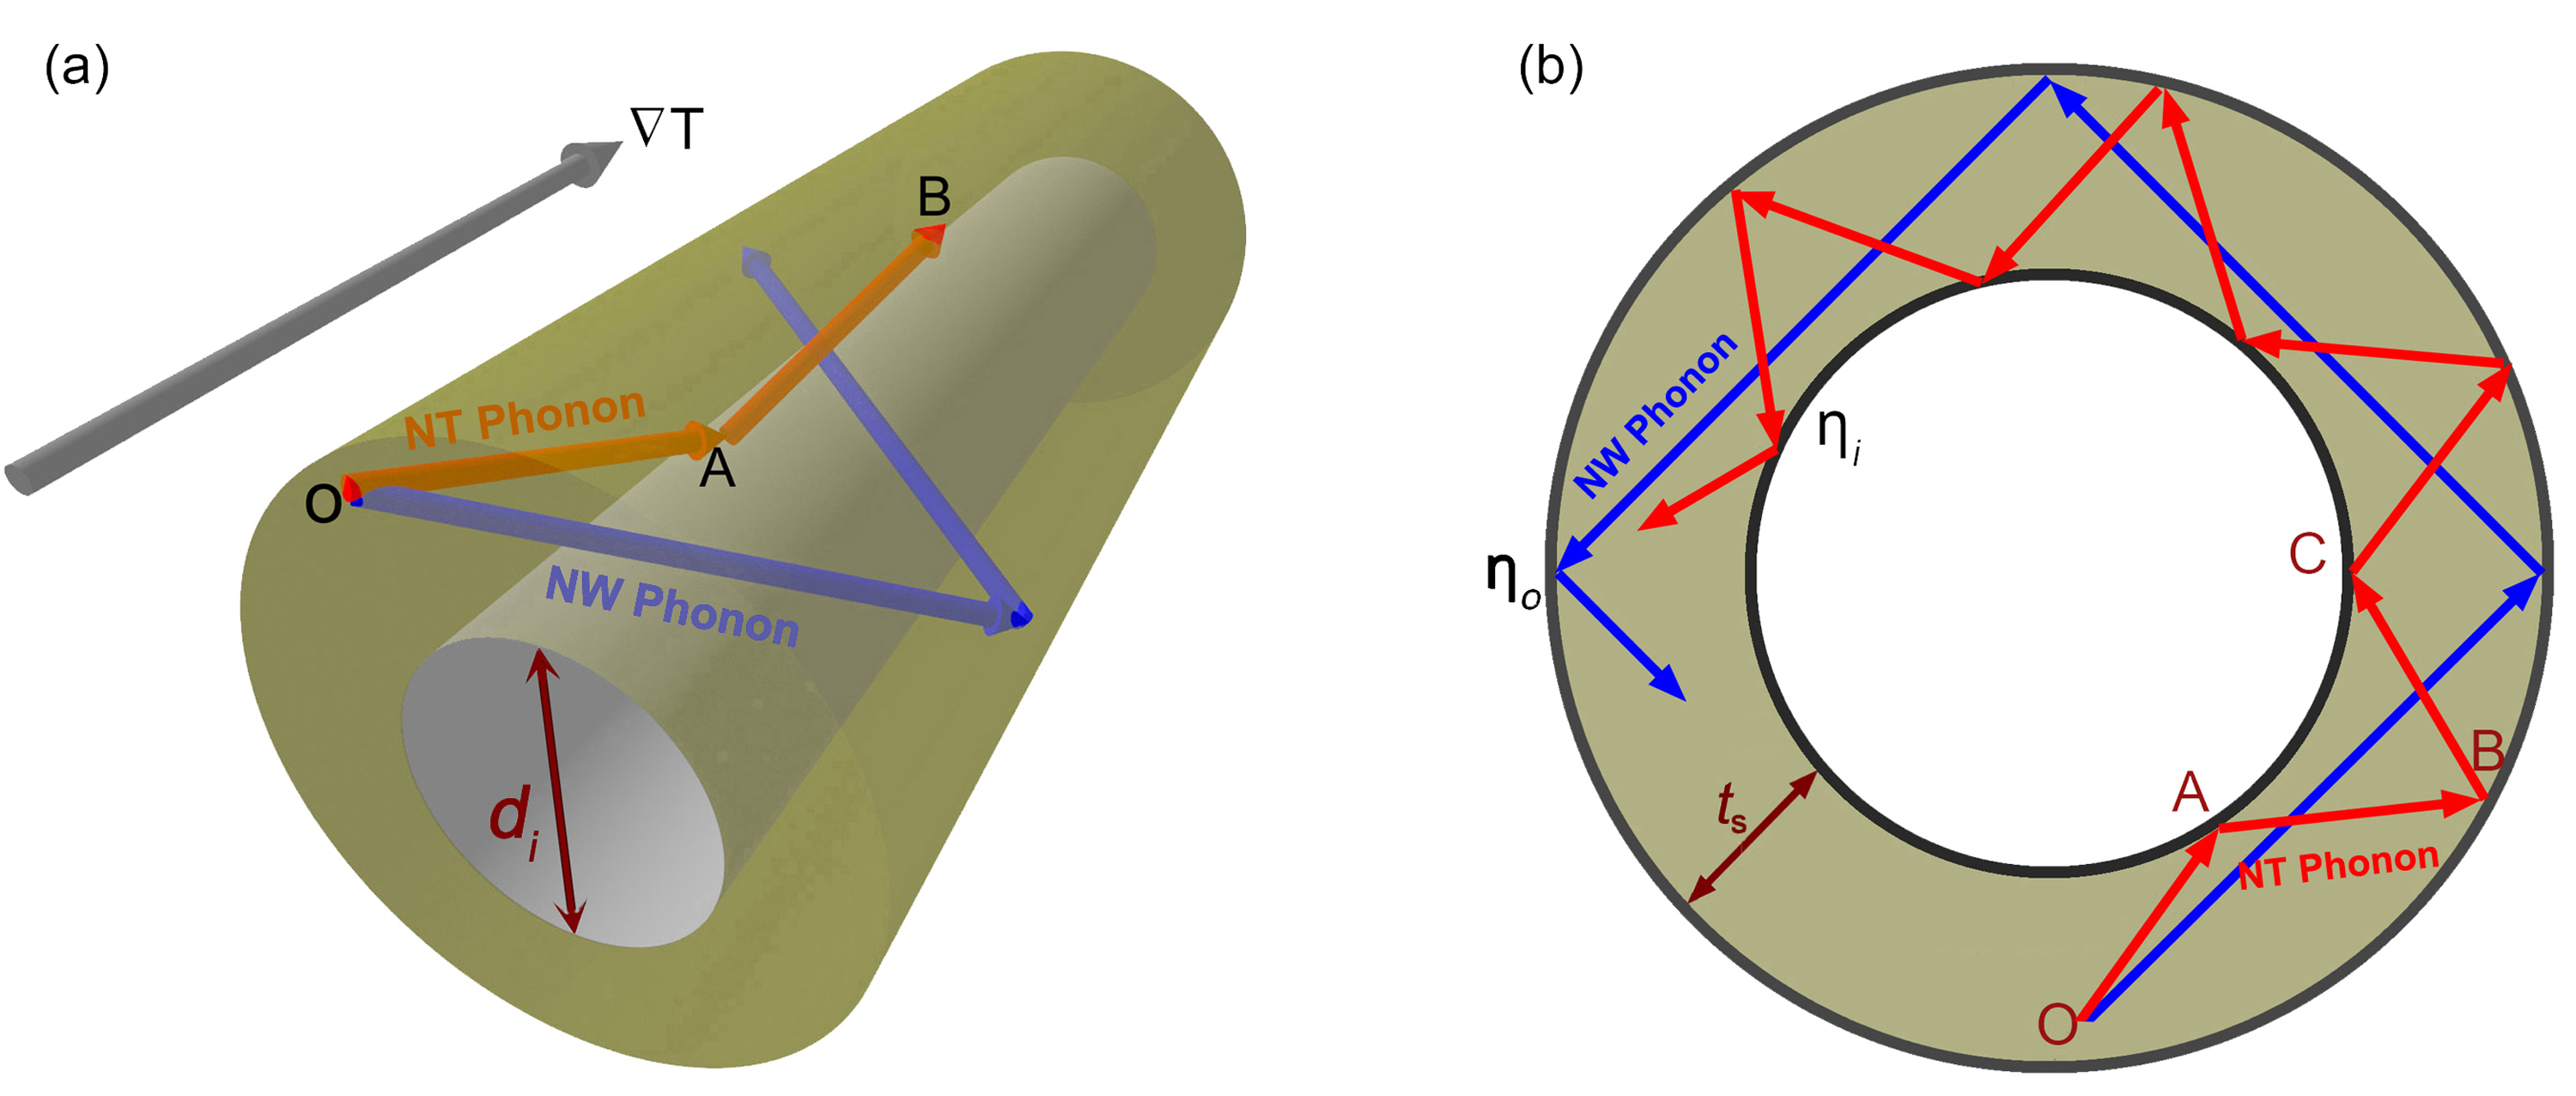
\includegraphics[width=0.95\textwidth]{/ch4/Figure1.jpg}
	\caption{Schematic representations of NT (red) and NW (blue) phonons within a nanotube. (a) NT phonons interact with both inner and outer surfaces while NW phonons interact only with the outer surface. (b) Cross-sectional view of the nanotube with the projections of the phonon trajectories.}
	\label{fig:nt_schematic}
\end{figure}

We show in \Cref{fig:nt_schematic}, a nanotube with inner diameter \gls{di} and outer diameter \gls{do}, creating a silicon shell of thickness \gls{ts}. We note that in a nanotube there are inner and outer surface boundaries which in general can have distinct characteristics from each other. Phonons in nanotubes can be classified on the basis of the presence (or absence) of interaction with the inner boundary based on their angle of propagation and point of origin O within the nanowire. \emph{Phonons that interact with both the inner and outer boundaries are termed as NT phonons and are shown with red arrows, while phonons that propagate unperturbed by the presence of the inner silicon-air interface are termed as NW phonons and shown with blue arrows}. The thermal gradient is applied along the axial direction of the nanotube. \Cref{fig:nt_schematic}(b) is the two-dimensional projection of the phonon transport within a nanotube showing the successive reflections of phonons at the surfaces for both NT and NW phonons. At each of these phonon-surface interactions, part of the thermal energy is specularly reflected while part is lost due to diffusive phonon scattering occurring at the surfaces. We note that our model can selectively incorporate this fundamental difference between the propagation properties of NT and NW phonons in addition to the specific surface scattering properties at the internal and external boundaries. Prediction of thermal transport properties such as thermal conductivity in nanotubes requires analysis of both NT and NW phonon contributions to thermal energy transport. The thermal transport properties of NT phonons are captured via a novel formalism accounting for the reduction in their mean-free-paths upon interaction with the inner and outer boundaries each with its individual specularity \gls{p}$_{in}$ and \gls{p}$_{out}$, respectively. Note that this model of NT phonons is directly derived from the method for asymmetric thin-films shown in \Cref{sec:ch3-method}. At every phonon-outer boundary scattering, $1 - $\gls{p}$_{out}$ proportion of phonons are scattered diffusively, while $1 - $\gls{p}$_{in}$ are diffusively scattered at the inner boundary. For NT phonons with initial propagation direction towards the outer nanotube boundary, the reduced phonon mean-free-paths are calculated as follows,

%Equations here


%\begin{equation}
\begin{align}\label{eq:nt_mode}
\ell_{\vec{k},r,\theta,\textrm{surface-properties}}^{\textrm{NT-mode}} =
&\overbrace{ \int_{0}^{\Lambda}{\frac{r}{\ell_{\vec{k}}^{\textrm{bulk}}}e^{-\frac{r}{\ell_{\vec{k}}^{\textrm{bulk}}}}\,dr} +(1-p_{\textrm{out}})\int_{\Lambda}^{\infty} {\frac{\Lambda}{\ell_{\vec{k}}^{\textrm{bulk}}}e^{-\frac{r}{\ell_{\vec{k}}^{\textrm{bulk}}}}\,dr} }^\text{1st Scattering Event}  \nonumber \\
+&\overbrace{p_{\textrm{out}} \int_{\Lambda}^{\Lambda+\Lambda^{*}}{\frac{r}{\ell_{\vec{k}}^{\textrm{bulk}}}e^{-\frac{r}{\ell_{\vec{k}}^{\textrm{bulk}}}}\,dr} +p_{\textrm{out}}(1-p_{\textrm{in}})\int_{\Lambda+\Lambda^{*}}^{\infty} {\frac{\Lambda+\Lambda^{*}}{\ell_{\vec{k}}^{\textrm{bulk}}}e^{-\frac{r}{\ell_{\vec{k}}^{\textrm{bulk}}}}\,dr} }^\text{2nd Scattering Event}\nonumber \\
+&\overbrace{p_{\textrm{out}}p_{\textrm{in}} \int_{\Lambda+\Lambda^{*}}^{\Lambda+2\Lambda^{*}}{\frac{r}{\ell_{\vec{k}}^{\textrm{bulk}}}e^{-\frac{r}{\ell_{\vec{k}}^{\textrm{bulk}}}}\,dr} +p_{\textrm{out}}p_{\textrm{in}}(1-p_{\textrm{out}})\int_{\Lambda+2\Lambda^{*}}^{\infty} {\frac{\Lambda+2\Lambda^{*}}{\ell_{\vec{k}}^{\textrm{bulk}}}e^{-\frac{r}{\ell_{\vec{k}}^{\textrm{bulk}}}}\,dr} }^\text{3rd Scattering Event}\nonumber \\
+&{\dots}
\end{align}
%\end{equation} 
%!!!!!!!!!!!

where the specularities $p_{in}$ and $p_{out}$ of inner and outer nanotube surfaces depend on \gls{k}, \gls{r}, \gls{eta}, and \gls{cl} i.e. phonon wave number and angle of propagation \gls{theta}, spatial position along the propagation direction, surface roughness and correlation length, respectively. The symbols $\Lambda = OA$, $\Lambda^{*} = AB (=BC)$ correspond to the distances depicted in \Cref{fig:nt_schematic}(b). The reduced mean-free-paths for phonons with their initial propagation direction towards the inner surface can be analogously evaluated by exchanging $p_{in}$ and $p_{out}$ in \Cref{eq:nt_mode}. Note that the sum over infinitely large number of scattering events determines the reduced mean-free-path of the NT phonons. In contrast to NT phonons, the thermal transport properties of NW phonons, as their name suggests, are similar to those in nanowires (see \Cref{chap:predictive}) since in this case the phonons are unperturbed by the presence of the inner boundary of the nanotube [blue modes in \Cref{fig:nt_schematic}(b)]. For NW phonons, a simpler expression for the reduced mean-free-paths can be obtained similar to \Cref{eq:ch2-mfp_reduced}.

The interaction of phonons with the nanostructure boundaries is the key factor that allows for a control over thermal transport properties at the nanoscale and their modification from bulk values. The influence of boundaries on thermal transport becomes stronger with reducing dimensions and the corresponding increase in surface-to-volume ratio. Thus, it is imperative to consider rigorous descriptions of phonon-boundary scattering to accurately predict thermal phonon transport. To describe the phonon-boundary interaction in the nanotube, we use the Beckmann-Kirchhoff surface scattering model and surface shadowing approach (detailed in \Cref{sec:BK}) to determine the surface specularity \gls{p}, which is the proportion of phonons that are specularly reflected upon interacting with a boundary (the proportion $1-p$ is diffusely scattered).

\section{Results and Discussion}
\subsection{Role of Shell Thickness}
A key indicator of phonon transport in nanostructures is the surface-to-volume ratio, and for nanotubes it is inversely proportional to the shell thickness \gls{ts}. Thus, we start our analysis by quantifying the impact of shell thickness on thermal conductivity \gls{K} by considering a pure Si nanotube and two silicon-germanium alloy nanotubes -- \sige{0.90}{0.10}, \sige{0.95}{0.05}, all with fixed outer diameter \gls{do} of 100 nm [\Cref{fig:nt_fig2}]. The outer diameter selection is similar to previously experimentally grown crystalline nanotubes \cite{RN436}. We fix the correlation length \gls{cl} to be ten times the roughness \gls{eta} for simplicity in analysis \cite{ownNW}.  We also consider bulk dispersion relations apply, as the coherent effects and quantum confinement are expected to be small at the temperature and structural conditions (thickness and roughness scales) considered in this study \cite{RN240,RN447}. Additionally, for the scattering from small proportion of Ge atoms in a Si host, we use effective medium approach based on Rayleigh scattering of phonons from a virtual crystal of Si and alloyed Ge. This approach has been shown to accurately provide the bulk SiGe thermal conductivity dependence on alloying with Ge \cite{RN132,RN289}. 

% Fig2
\begin{figure}[hbt]
	\centering 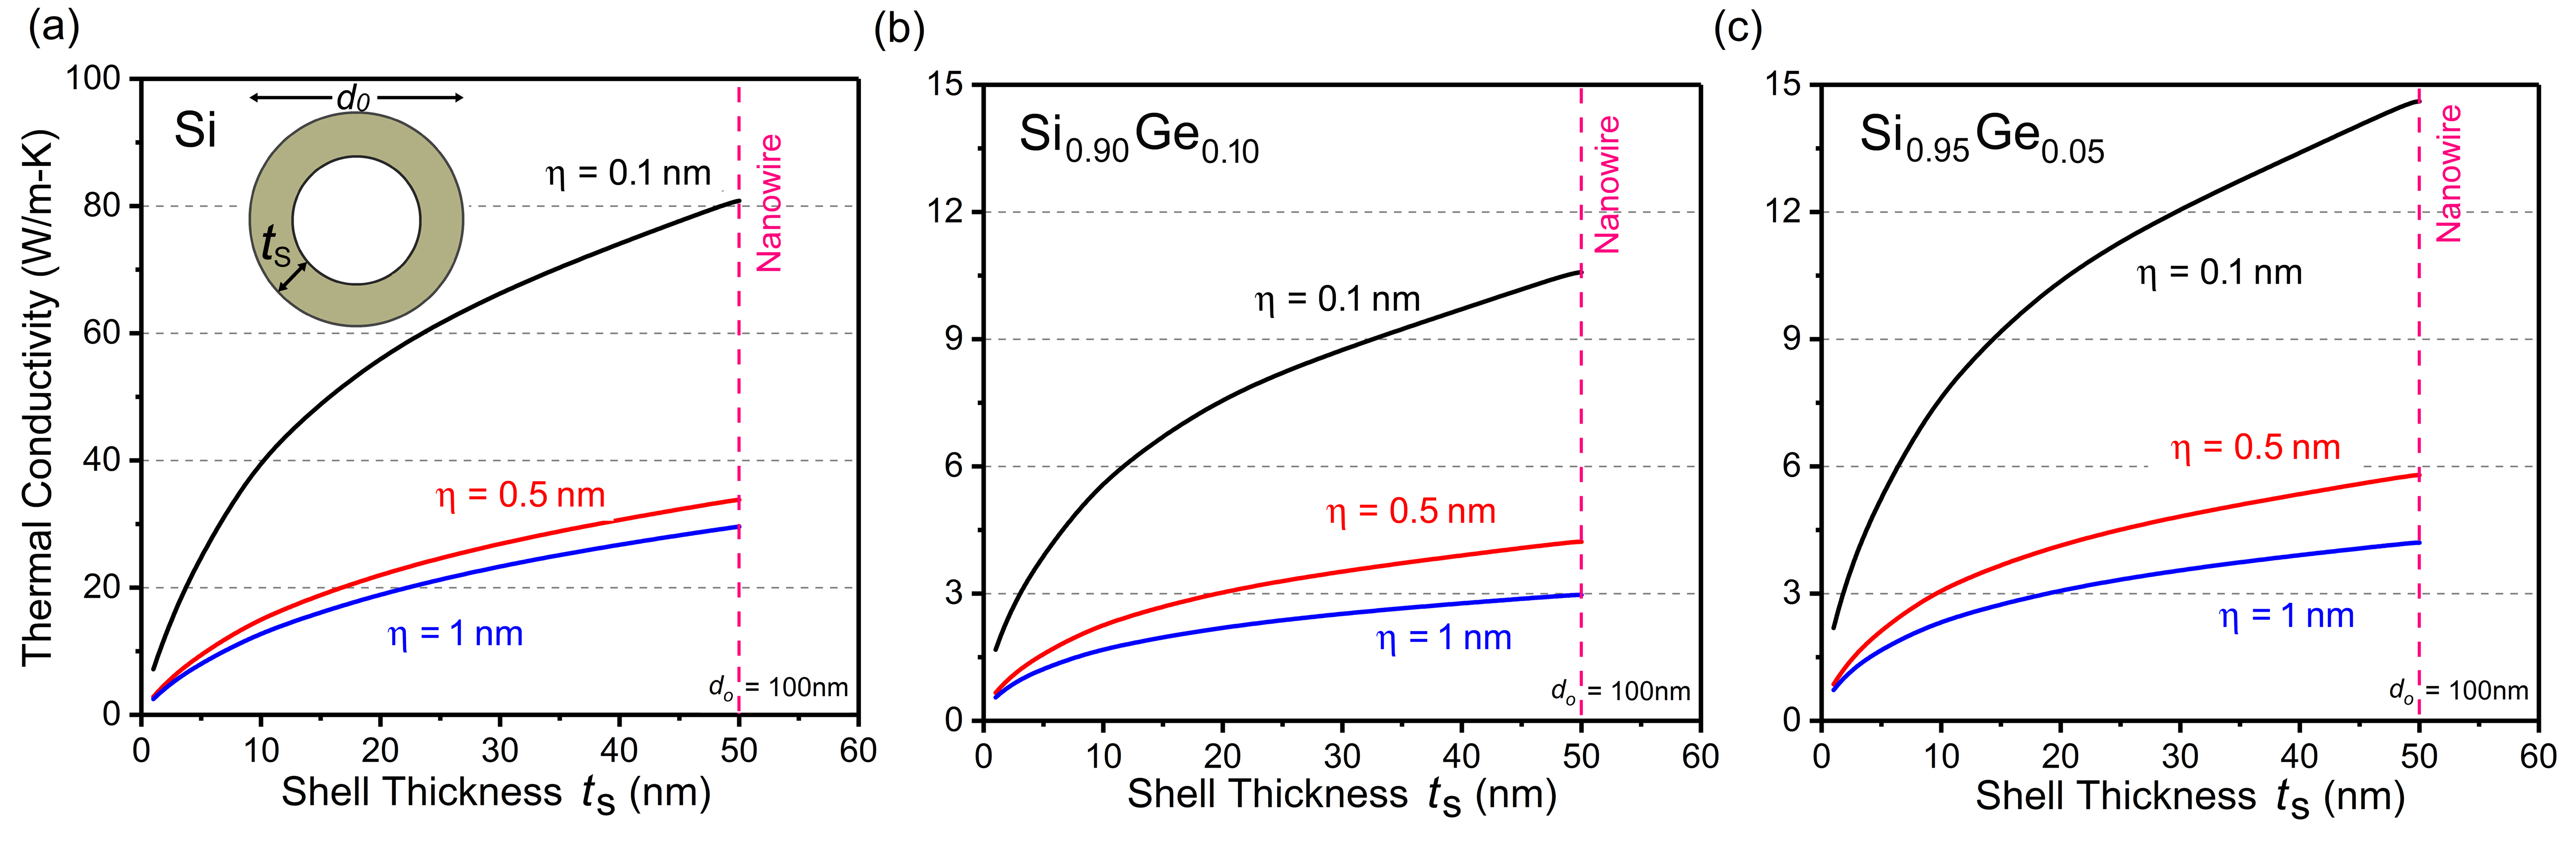
\includegraphics[width=\textwidth]{/ch4/Figure2.jpg}
	\caption{Thermal conductivity of nanotubes at room temperature as a function of shell thickness \gls{ts} for (a) crystalline silicon, (b) silicon nanotubes with 10\% alloyed germanium, and (c) silicon nanotubes with 5\% alloyed germanium. The outer diameter \gls{do} is 100 nm and the inner and outer boundaries are assumed to have identical surface properties \gls{eta}.}
	\label{fig:nt_fig2}
\end{figure}

We show in \Cref{fig:nt_fig2} how for all the cases increasing surface roughness reduces the thermal conductivity of the nanotube due to more diffusive scattering of phonons at boundaries. Additionally, we show that the reduction in nanotube shell thickness leads to a decreasing thermal conductivity owing to the increased surface-to-volume ratio. Note that, in contrast to nanowires, nanotubes provide an avenue to access lower thermal conductivity regimes even with large experimentally realizable outer diameters, making them a promising candidate for low thermal conductivity applications.


\subsection{Predictions of Thermal Spectra}

\begin{figure}[b!]
	\centering 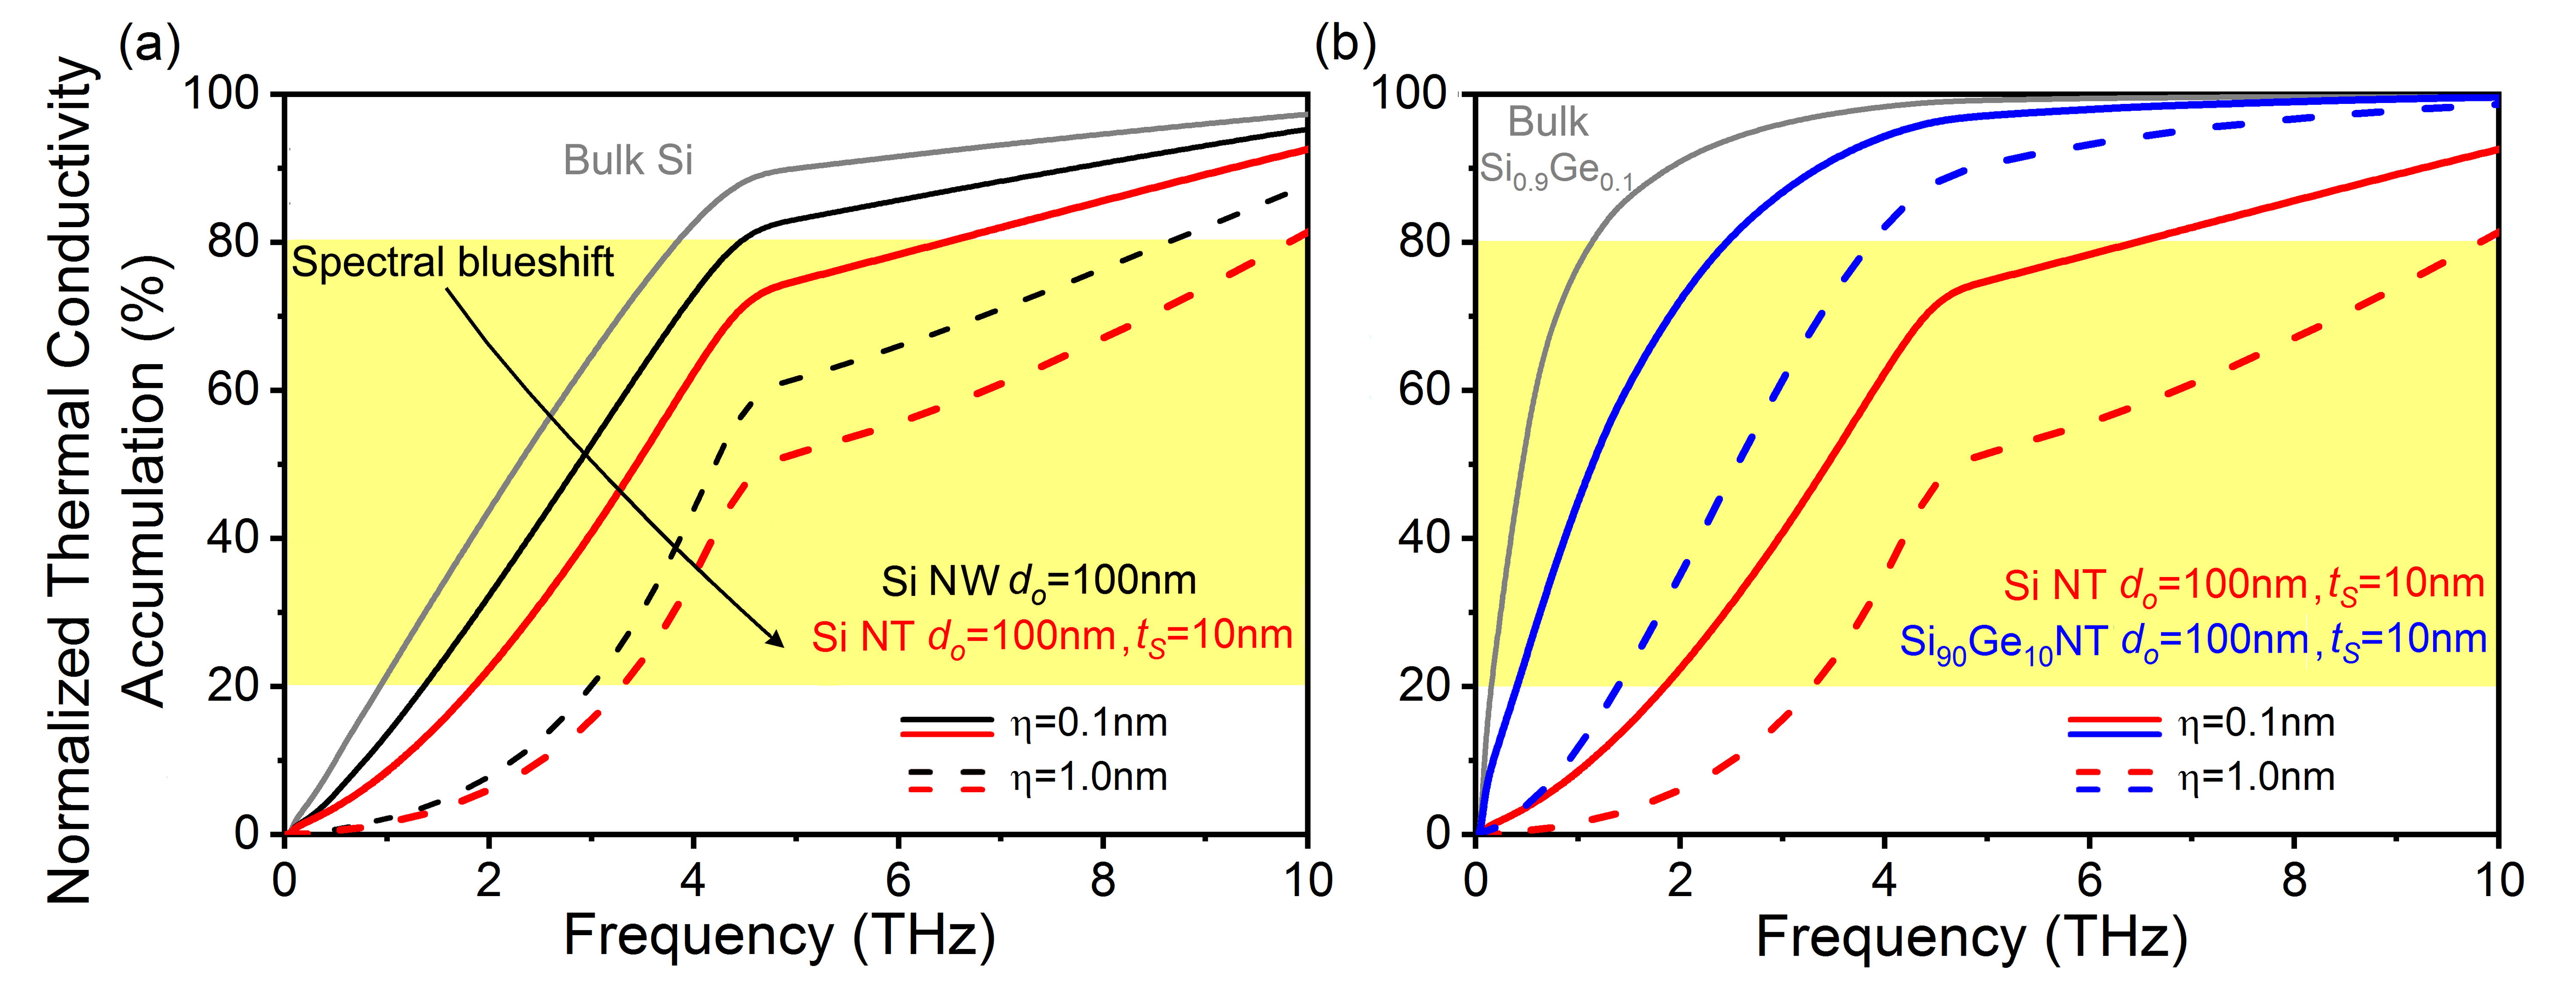
\includegraphics[width=\textwidth]{/ch4/Figure3.jpg}
	\caption{Frequency heat-spectra (or normalized thermal conductivity accumulation functions) for (a) bulk Si (gray line), 100 nm diameter Si nanowires (black), and Si nanotubes of outer diameter 100 nm and shell thickness 10 nm (red) at room temperature. The effect of alloying is shown in (b) where the spectra for bulk \sige{0.90}{0.10} is shown in gray and for an alloyed nanotube in blue. Si nanotubes are shown for reference in red as in (a). The solid and dotted lines represent surface roughnesses of \gls{eta} = 0.1 and \gls{eta} = 1.0 nm.}
	\label{fig:nt_fig3}
\end{figure}

\begin{figure}[b!]
	\centering 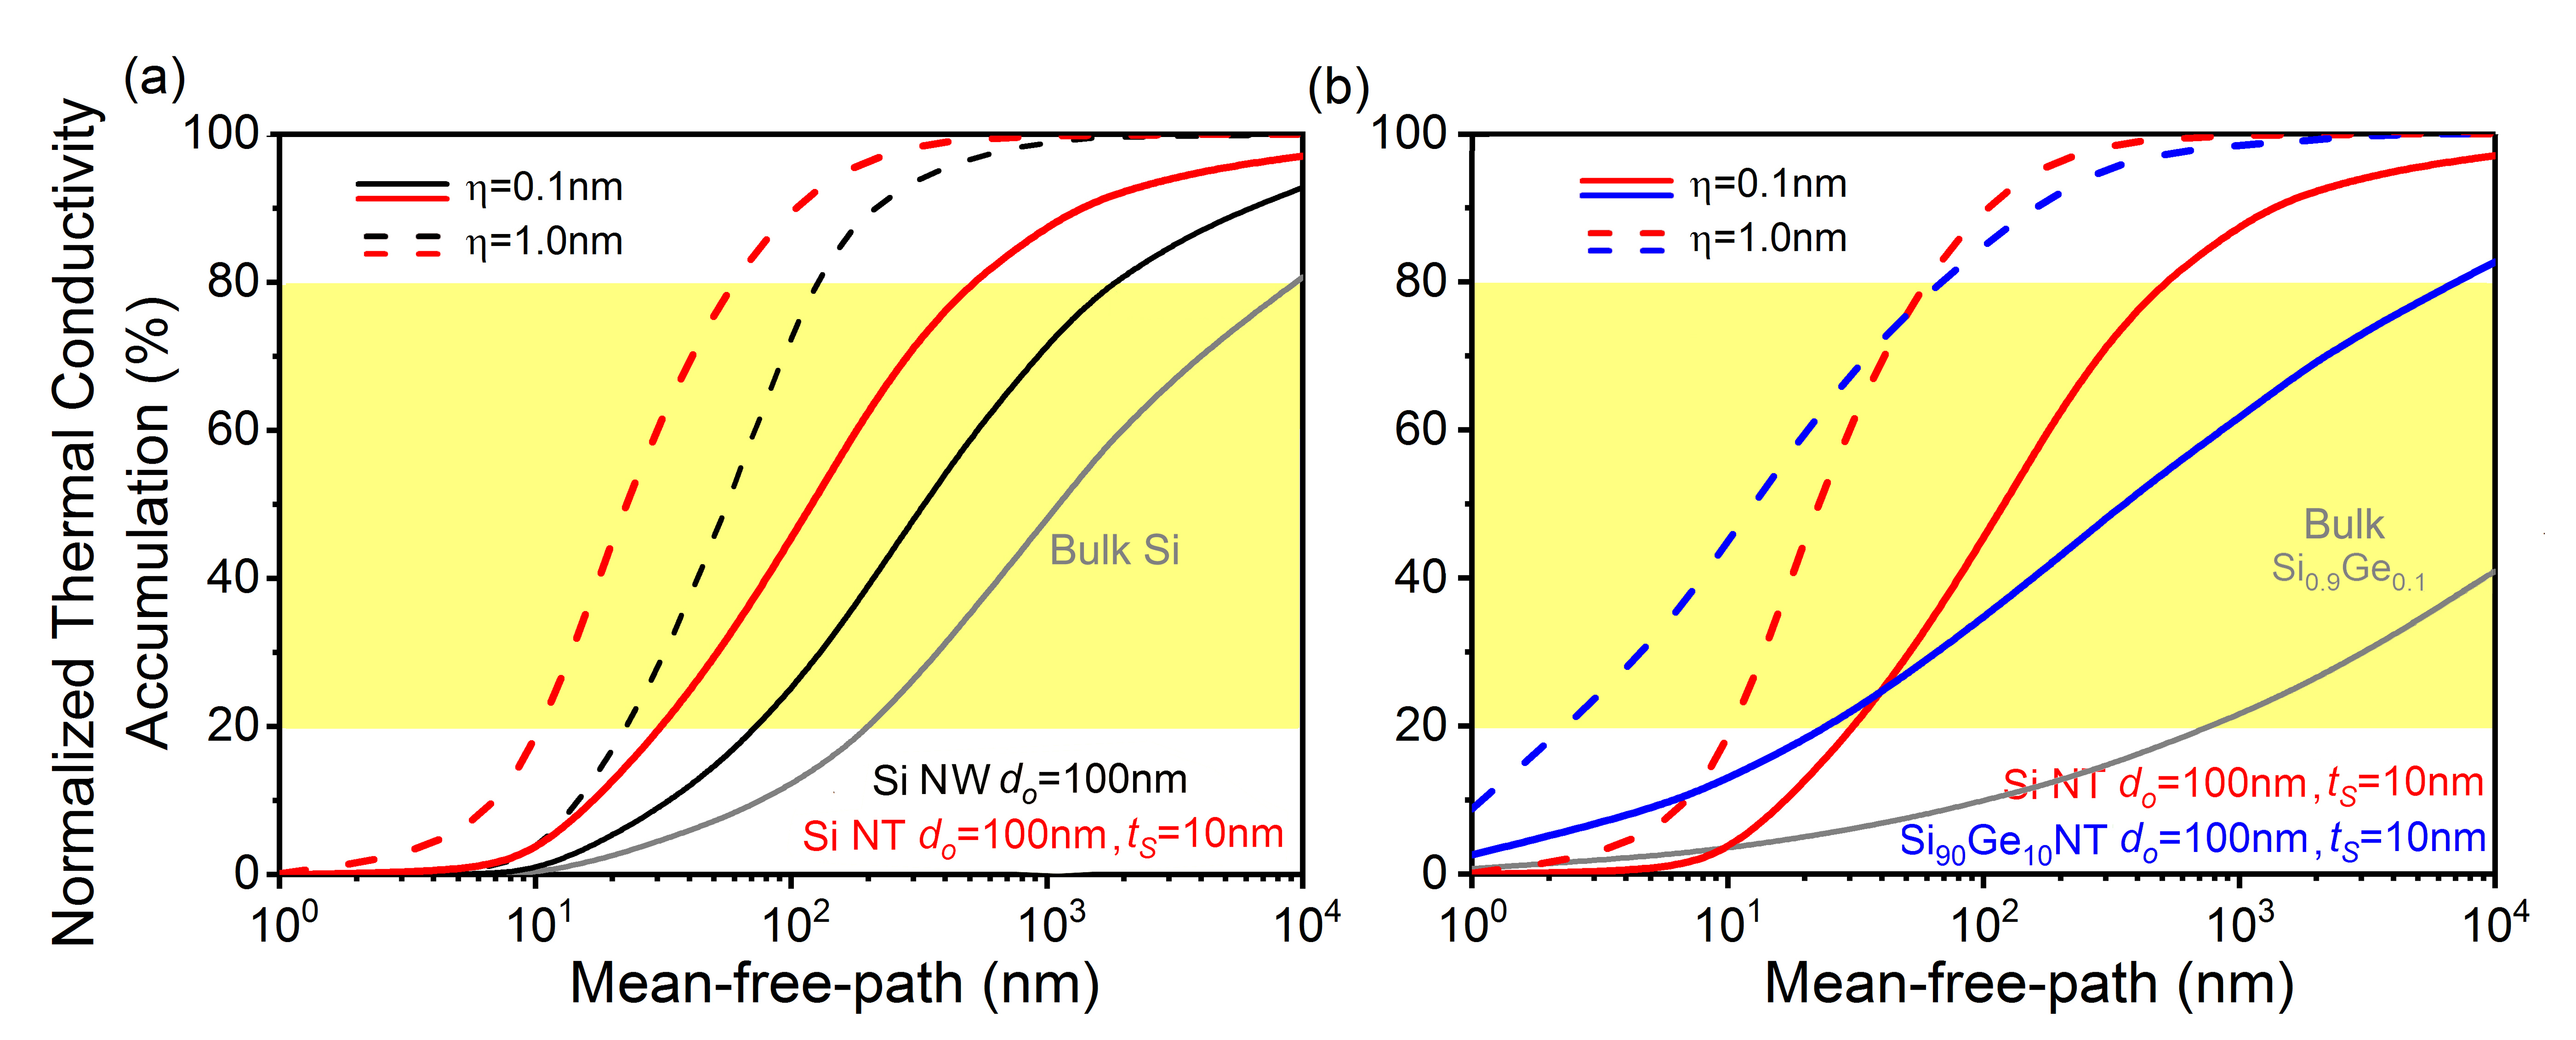
\includegraphics[width=\textwidth]{/ch4/Figure4.jpg}
	\caption{Mean-free-path heat spectra for (a) Si nanotubes (red) and nanowires (black) and (b) Si (red) and \sige{0.90}{0.10} nanotubes (blue) at \gls{T} = 300 K. Solid and dotted lines represent surface roughnesses of \gls{eta} = 0.1 nm and \gls{eta} = 1.0 nm, respectively. Bulk heat spectra are shown in gray.}
	\label{fig:nt_fig4}
\end{figure}

To elucidate the thermal transport mechanisms in nanotubes and understand the effects of impurity atoms in host lattice and surfaces, we next predict and analyze the frequency and mean-free-path thermal conductivity accumulation functions for several different structural and physical nanotube conditions. These heat spectra are the foundational basis for designing thermal materials for targeted applications (see \Cref{sec:pred_thermalspectra}). Starting with bulk Si, our calculations show that at room temperature, the addition of alloy atoms impacts the amount of heat carried by high frequency phonons strongly, moving the middle 60\% of heat spectra from the range 1–4 THz [\Cref{fig:nt_fig3}(a), solid gray line] to low frequency phonons with frequencies $<$ 1 THz [\Cref{fig:nt_fig3}(b), solid gray line]. That is, there is \emph{red shift} in the phonon frequency spectrum. The mean-free-path spectra for bulk Si [\Cref{fig:nt_fig4}] shows a corresponding shift towards larger mean free paths when Ge alloy atoms are present. We note that with Ge alloying, phonons with smaller mean-free-paths (also, higher frequencies) 	are scattered efficiently due to Rayleigh scattering by impurities (i.e. $\tau\!\sim\!\omega^{4}$), causing the proportion of heat transported by large mean-free-path phonons to increase. For example, we find that for alloyed nanotubes with smooth surfaces, 20\% of heat is carried by phonons of mean-free-paths larger than 10 $\mu$m in agreement with results from nanowires (see \Cref{chap:predictive}). In addition to alloying, surface scattering provides an extra degree to further tailor the frequency and mean-free-path heat spectra. For example, a Si nanowire of outer diameter \gls{do} = 100 nm and roughness \gls{eta} = 0.1 nm [\Cref{fig:nt_fig3}(a), solid black line] has its heat spectra blue-shifted to high frequencies with respect to bulk silicon [\Cref{fig:nt_fig3}(a), solid gray line]. The corresponding mean-free-path spectra moves towards smaller mean-free-paths. This blue-shift in heat spectra arises due to the presence of phonon-boundary scattering, which primarily reduces the mean-free-path of low-frequency phonons since high-frequency phonons have short mean-free-path phonons and are not able to interact with the boundaries. Importantly, nanotubes allow leveraging the phonon-boundary scattering mechanisms to strongly manipulate the heat spectra. For instance, a Si nanotube of the same outer diameter \gls{do} of 100 nm and roughness 0.1 nm on inner and outer boundaries and with a shell thickness \gls{ts} = 10 nm [\Cref{fig:nt_fig3}(a) and \Cref{fig:nt_fig4}(a), solid red line] shows a stronger blue shift to higher frequencies and shorter mean-free-paths than a nanowire of the same outer diameter. Furthermore, the effect of increasing roughness tends to blue shift the spectra to high frequencies as evidenced by the spectra of a nanotube with 1 nm roughness on both inner and outer boundaries \Cref{fig:nt_fig3}(a) and \Cref{fig:nt_fig4}(a), dashed red line]. Small surface roughness is therefore more appropriate from a thermal wave-effect perspective, as lower frequencies and larger mean-free-paths are better suited for coherent phonon manipulation in nanostructured materials. Note that SiGe alloy nanotubes can help to reduce the thermal phonon frequencies with respect to Si nanotubes [\Cref{fig:nt_fig3}(b), blue vs red lines], while preserving a long range of mean-free-paths [\Cref{fig:nt_fig4}(b), blue lines]. For instance, in Si NT with surface roughness \gls{eta} = 1 nm, the middle 60\% of heat is carried by phonons of $\sim$ 3–10 THz frequency range and 10–60 nm mean-free-path range. With alloying, the frequency range red-shifts to 1.5–4 THz, while mean-free-paths shift to 3–70 nm.


\subsection{Role of Different Inner and Outer Surface Conditions}

\begin{figure}[t!]
	\centering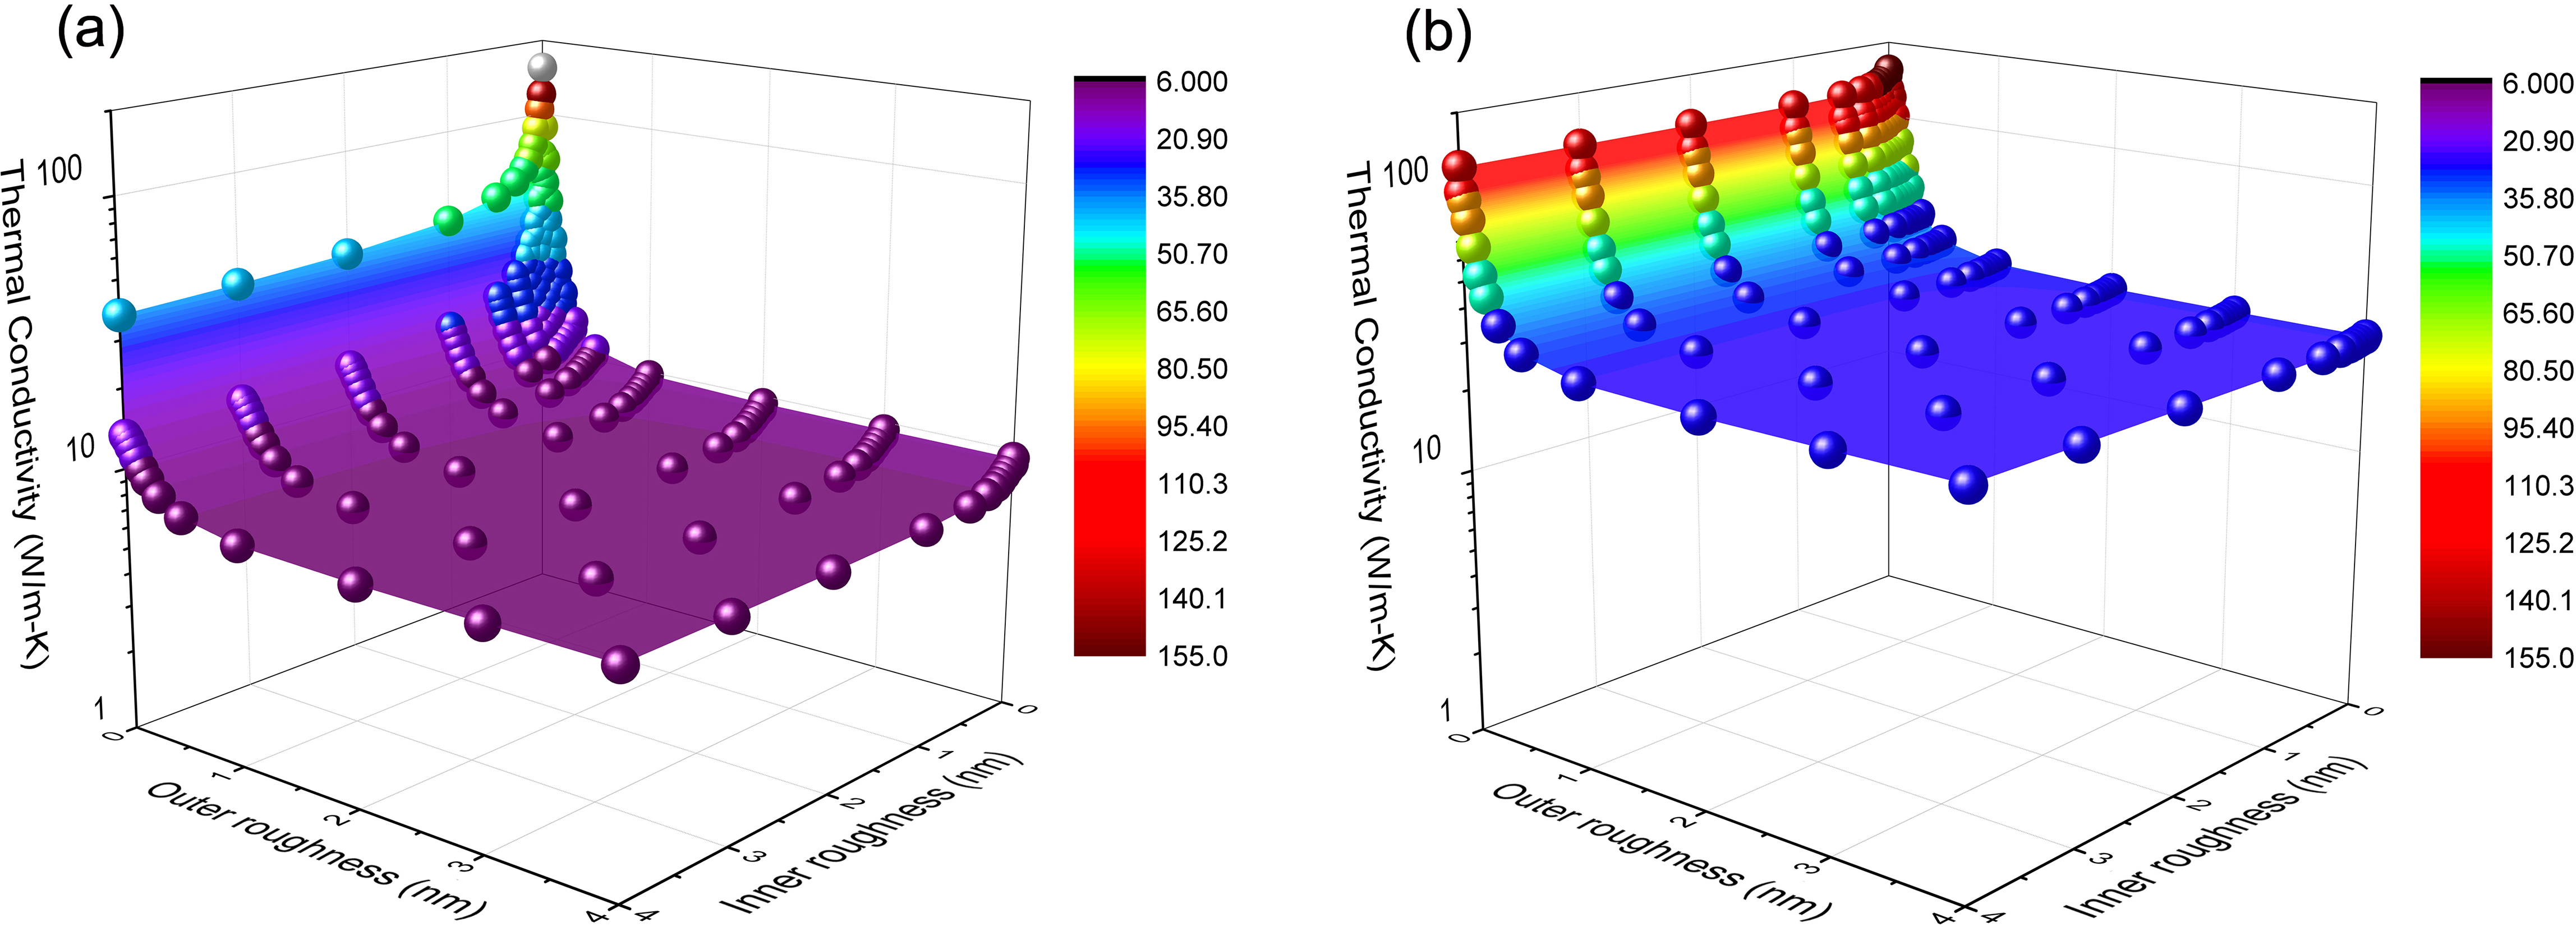
\includegraphics[width=\textwidth]{/ch4/Figure6.jpg}
	\caption{Thermal conductivity of Si nanotubes as a function of both inner and outer surface roughness \gls{eta}$_{in}$ and \gls{eta}$_{out}$ with (a) shell thickness \gls{ts} = 4 nm and (b) shell thickness \gls{ts} = 40 nm. Both nanotubes have outer diameter \gls{do} = 100 nm.}
	\label{fig:nt_fig6}
\end{figure}

Since in general the inner and outer surface nanotube surfaces could be exposed to different processing conditions, we next study phonon thermal transport in nanotubes where the inner and outer surfaces have different roughnesses. We consider two nanotubes: a thin shell nanotube with \gls{ts} = 4 nm and a thicker nanotube with \gls{ts} = 40 nm. The outer diameter for the thin shell nanotube is \gls{do} = 100 nm, similar to experimental grown nanotubes \cite{RN436}. The choice of these nanotubes allows for an analysis over a wide spectrum of structural dimensions. For a thin-shell nanotube (i.e. \gls{ts} = 4 nm) [\Cref{fig:nt_fig6}(a)] the thermal conductivity is more affected by the inner roughness in contrast to a nanotube with thicker outer shell (i.e., \gls{ts} = 40 nm) [\Cref{fig:nt_fig6}(b)]. The differential influence of inner boundary properties on thermal conductivity arises due to higher number of NT phonons in a thinner shell nanotube than a thicker nanotube. In a thicker shell nanotube, NW phonons, which remain unperturbed by the presence of inner surface conditions, are in higher proportions. It can also be observed that the thermal conductivity of Si nanotubes reduces with increasing roughness of surfaces, approaching a saturation roughness (or asymptotic behavior) indicative of the onset of nearly fully diffusive surface ($p_{in}\sim p_{out}\sim 0$). The saturation roughness is expected to be a function of the temperature following the mean-free-path heat spectra described previously. At room temperature this saturation roughness value is found to be in the order of \gls{eta} $\sim$ 2 nm. 

\begin{figure}[hbt]
	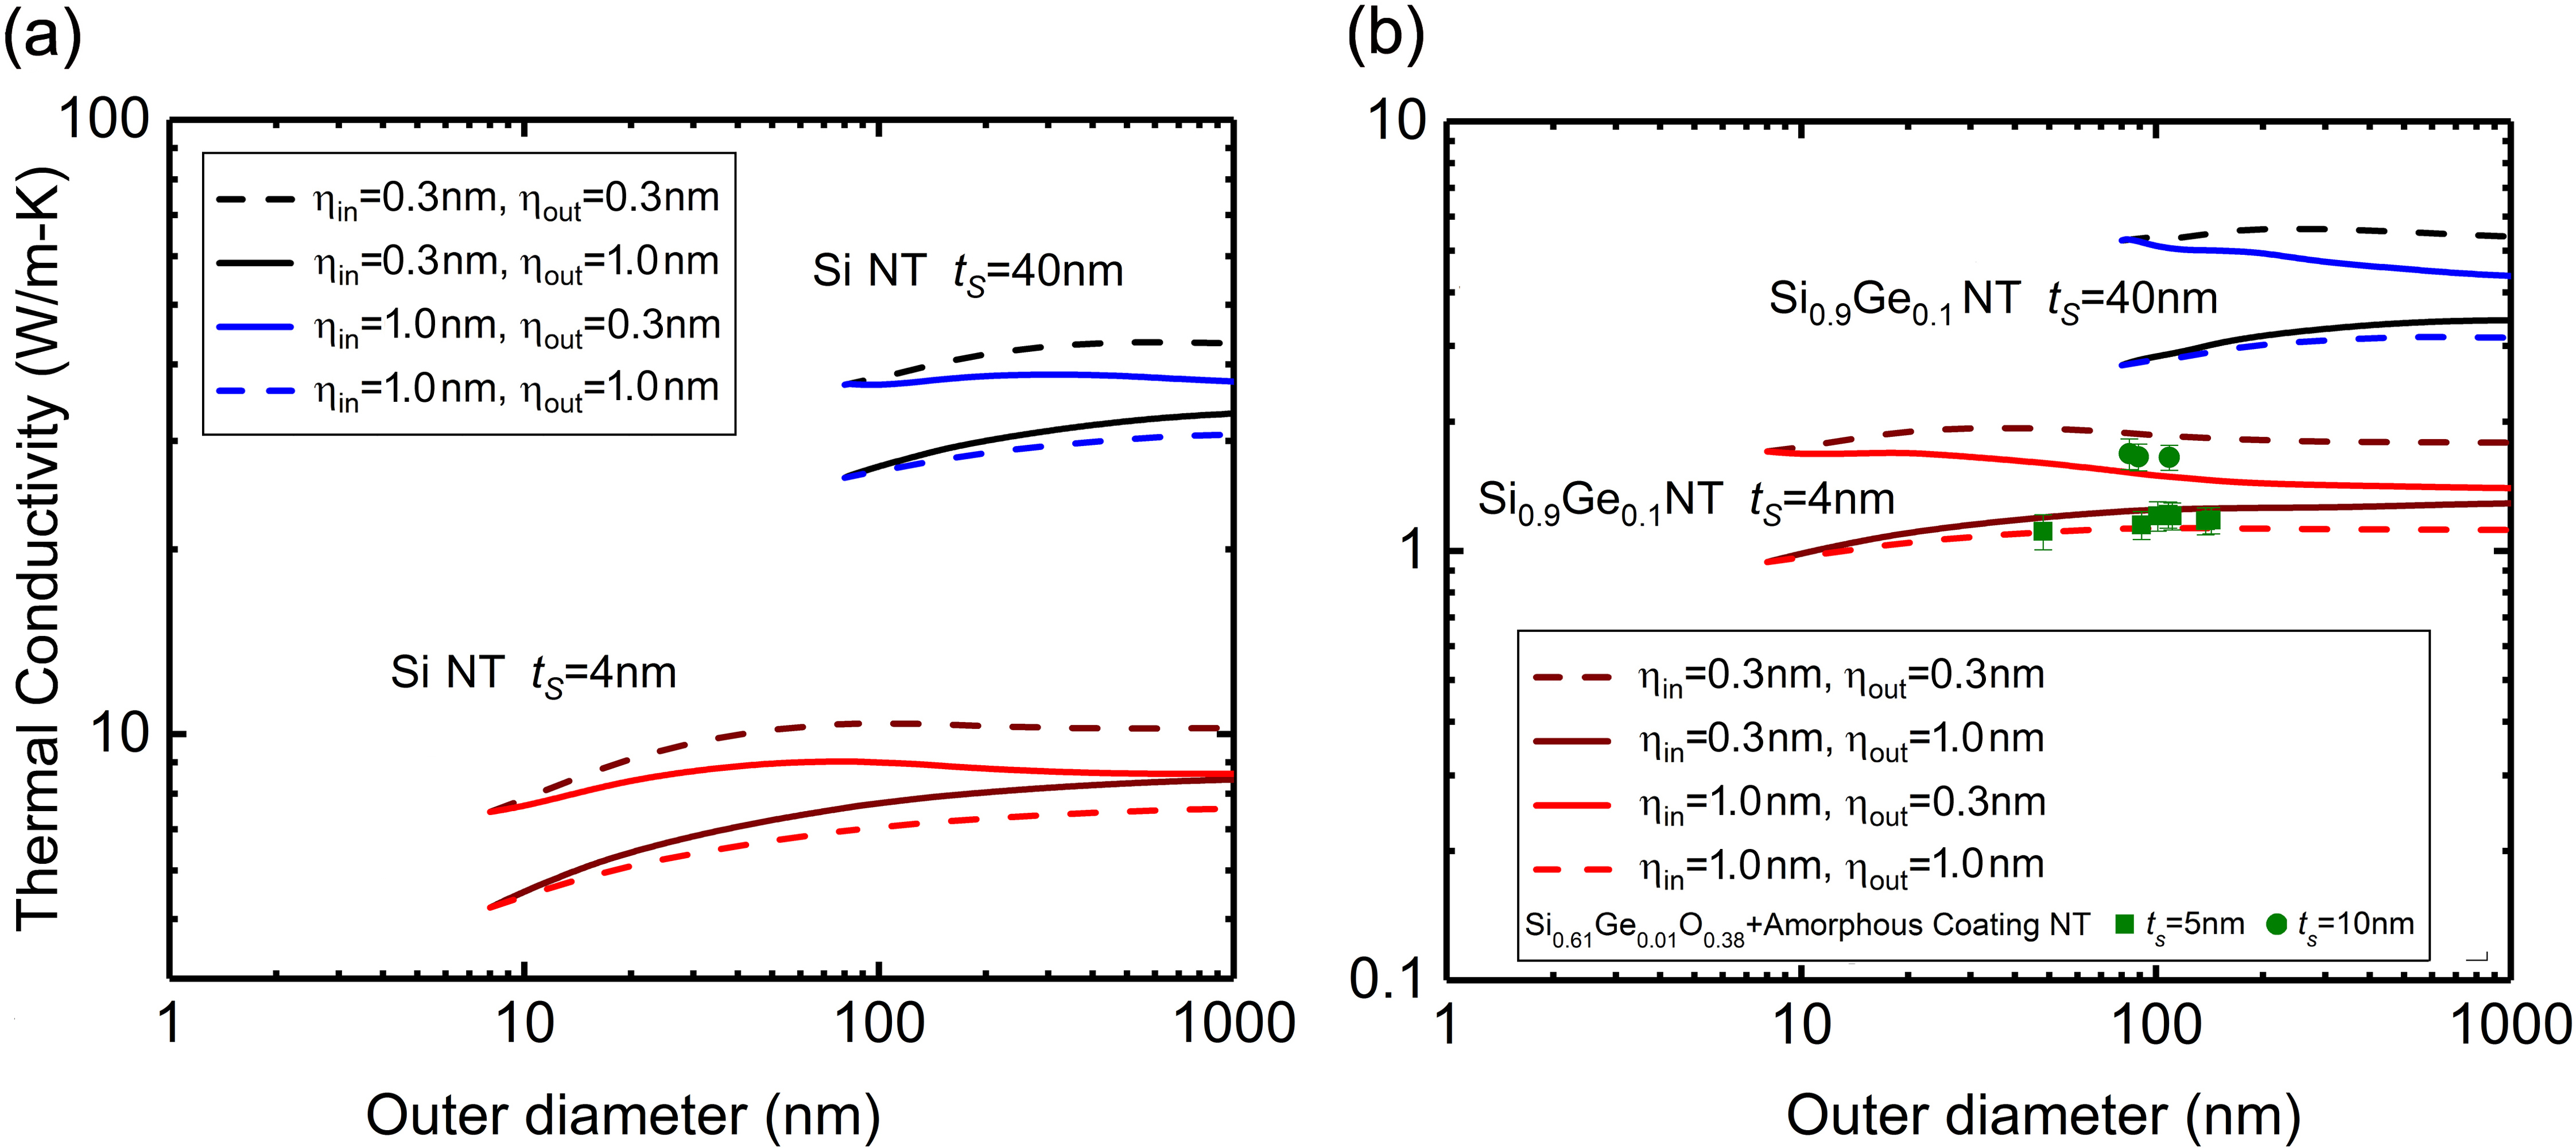
\includegraphics[width=\textwidth]{/ch4/Figure7.jpg}
	\caption{The thermal conductivity for (a) Si nanotubes and (b) \sige{0.90}{0.10} nanotubes as a function of outer diameter with varying surface roughnesses. Black and blue lines correspond to thicker shell (\gls{ts} = 40 nm) nanotube while wine and red lines correspond to thinner shell nanotube (\gls{ts} = 4 nm).}
	\label{fig:nt_fig7}
\end{figure}

To understand the correlation between the outer diameter, surface properties, and thermal conductivity, we next fix the shell thickness \gls{ts} as 4 nm and 40 nm while varying the outer diameter for Si [\Cref{fig:nt_fig7}(a)] and \sige{0.90}{0.10} [\Cref{fig:nt_fig7}(b)] nanotubes. The starting point of every curve at small outer diameters corresponds to the thermal conductivity when the inner diameter approaches zero (i.e. when the nanotube approaches a nanowire). In both Si and \sige{0.90}{0.10} nanotubes, the effect of a higher surface roughness leading to a lower thermal conductivity than smoother surface nanotube is observed. The thermal conductivity for the cases with two surfaces having distinct roughnesses (solid lines) are different from one another and show differential sensitivity to changing outer diameter highlighting the role of individual properties. The conductivity behavior with diameter in both these cases is a consequence of changing proportion of NT and NW modes in these structures, since for a fixed shell thickness, a larger outer diameter causes more phonons to interact with the inner surface transforming more NW phonons to NT phonons. We note that the sensitivity of thermal conductivity to increasing outer diameter for thin nanotubes is diminished as they begin to approach a ‘thin-film’ like structure \cite{RN431}.

\section{Summary}
We analyzed the behavior of thermal energy transport in an emerging class of one-dimensional nanomaterials viz. semiconductor nanotubes. Using frequency-dependent phonon properties and quantifiable surface properties, we presented a rigorous physical description of heat conduction that captures the underlying phonon dynamics in these novel nanostructures. Our model allowed us to evaluate nanotube thermal conductivities for a wide range of material and structural properties including alloying, outer diameters, shell thicknesses and temperatures; \emph{while preserving the ability to treat the two surfaces independently with their distinct roughnesses}. The independent treatment of the two surfaces was used to explain their differential role in thermal transport in these nanostructures. We concluded that in general, the thermal conductivity of the nanotube depends on the outer diameter even for the same shell thickness. We showed that the experimentally observed independence between these quantities could be explained by a combination of addition of impurity atoms to the Silicon lattice and surface roughness. The frequency and mean-free-path heat spectra showed in this thesis are a critical step towards fully discerning thermal conduction in these nanostructures and moving towards a guided material design. The methodology and the results of this chapter provide a fundamental understanding into thermal transport phenomenon in low-dimensional nanotube structures.







%%%%%%%%%%%%%%%%
% Chapter 5
%%%%%%%%%%%%%%%%

%!TEX root = thesis.tex
\chapter{Phonon Coupling in Semiconductor Bi-layers and Tri-layers}
\label{chap:layered}
%INTRODUCTION%
\section{Introduction} \blfootnote{Portions of this chapter have originally been published in \cite{ownCoupling1} ``Enhancing Thermal Transport in Layered Nanomaterials" (2018), \textit{Scientific Reports}, Vol. 8 (1880); in \cite{ownCoupling2} ``Modulating Thermal Conduction via Phonon Spectral Coupling" (2018), \textit{Journal of Applied Physics}, Vol. 124 (124302); and in \cite{ownKK1} ``Unconventional Thermal Transport in Thin Film-on-Substrate Systems" (2018), \textit{Journal of Physics D: Applied Physics}, Vol. 51 (365302). Reproduced from \cite{ownCoupling1} under a CC BY 4.0 License, from \cite{ownCoupling2} with permission from AIP Publishing, and from \cite{ownKK1} with permission from IOP Publishing.}
The ability to reduce heat conduction at nanoscale has been propelled by advances in the understanding of phonon transport processes in semiconductors. In recent years, suppression of thermal conduction by orders of magnitude has been achieved through the diffuse scattering of phonons at nanostructure surfaces. Nanowires, thin-films, nanotubes, superlattices, polycrystals, and nanocomposites with extremely low thermal conductivities have been introduced which find applications as efficient thermoelectric materials \cite{RN136,NW_hochbaum,RN417,RN29,RN88,RN158,RN320,RN132,RN394,RN393,RN240,RN294,ownNW,ownTF,ownSpatialTF}. Nanostructuring has thus primarily been used to reduce the thermal conductivities for a wide range of temperatures, and was the underlying motivation of \Cref{chap:predictive,chap:diff_boundary,chap:nt}. 
\par However, under a rational material design paradigm to create thermal materials, it is paramount to possess the ability to achieve both very low and very high thermal conductivities. Accessing the ability to enhance thermal conduction at nanoscale requires the development of novel approaches based on a deep understanding of phonon transport behavior. Furthermore, progress in many technological areas is hinged upon enhancing thermal transport. For instance, the performance of micro- and nano-electronic devices is hindered by the creation of hot-spots and high working temperatures as small sizes limit efficient heat dissipation (see \Cref{chap:intro}). This need to obtain increased thermal conductivities has also motivated recent efforts to study the effects of interfacial disorder \cite{RN265}, extremely low temperature \cite{RN397}, and texturing of interfaces \cite{RN398} on changes in thermal conductance. Additionally, being able to devise physical mechanisms that would allow to increase thermal conduction is of crucial importance in the efficiency of electronic and optoelectronic devices. For example, long laser lifetimes necessitate an upper bound on the temperature of active layers thus making efficient heat removal a crucial aspect of designing laser systems \cite{ownKK1}. In addition, heat accumulation in the depletion layer of photo-detectors can lead to device failure at high optical power \cite{kk-li2003}. An increase in dark current with temperature leading to increased power dissipation can also result in thermal runaway and failure \cite{kk-Lorenzen2001}. In contrast to the extensive amount of work on achieving reduced thermal conduction in nano systems, approaches that can enhance thermal conduction have been limited. In particular, increased thermal dissipation in thin-films and layered nanomaterials would have a critical impact on performances of electronic and optoelectronic devices.
\par In this chapter, we formulate a mathematical model to study thermal transport in layered nanomaterials based on solving the BTE for non-equilibrium phonon populations. We briefly discussed such method in \Cref{chap:diff_boundary} for free-standing thin-films. Here, we show a more generic development that can account for both backward scattering (i.e., reflection) and forward scattering (i.e., transmission) of phonons at an interface between two nanostructured semiconductors. Using this model, we elucidate the role of phonon coupling on the local thermal conductivity of each layer in the structure. Specifically, we show the impact of phonon coupling on thermal conductivity of Si and Ge layers in a Si-Ge-Si tri-layer structure and highlight that phonon coupling can be used to enhance the thermal conductivity of the Ge layer. We analyze the root-cause of such an occurrence with our model and study the role of different structural parameters, including surface properties and layer sizes. Finally, we apply the model to technologically important structures, i.e. film-on-substrate architectures (FOS), and show that thermal conduction in these film-on-substrate systems is distinct from free-standing thin films highlighting the role of phonon coupling for design of devices and in interpreting read-out from experiments.
%METHOD
\section{Method}
%Figure
\begin{figure}[hbt]
  \centering 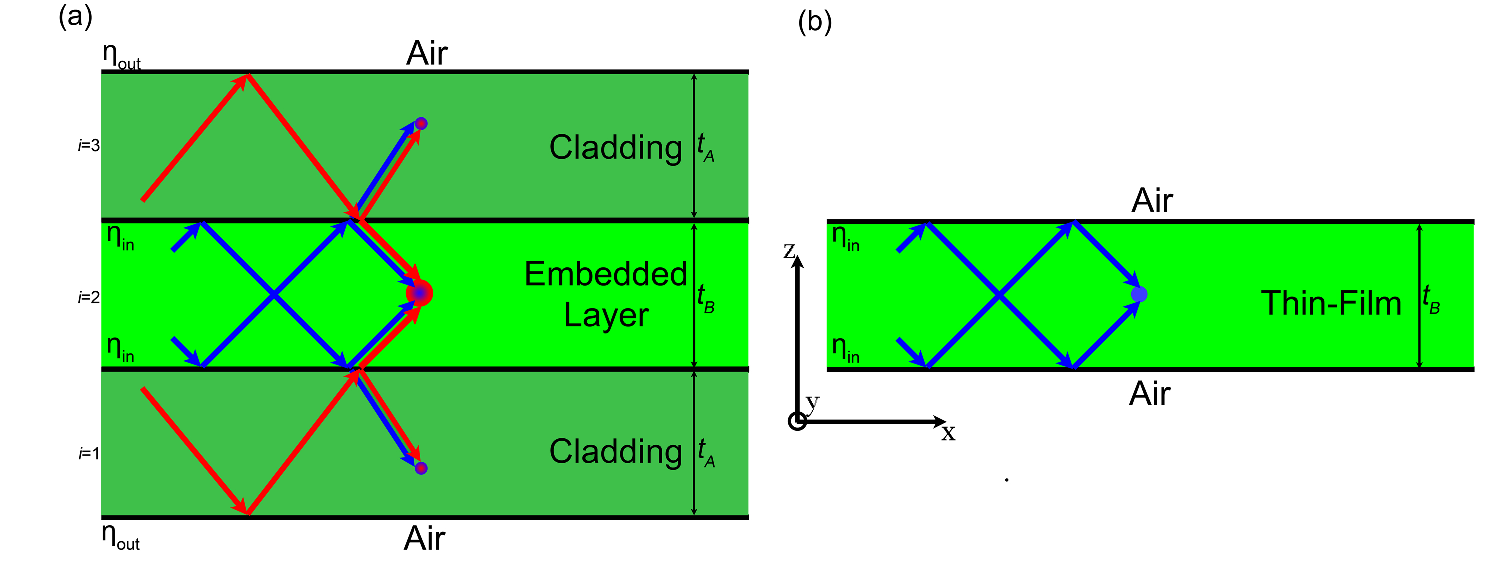
\includegraphics[width=1.0\textwidth,scale=1.5]{ch5/Fig1.pdf}
  \caption{(a) A tri-layer architecture (A-B-A) made of an embedded B layer with thickness $t_2$ and cladding A layers with thicknesses $t_1$. The roughness of the inner surface between embedded and cladding layers is $\eta_{in}$ and the roughness of the cladding-air outer interface is $\eta_{out}$. Arrows illustrate the phonon injection mechanism, wherein phonons from the cladding layers A couple across the inner interface to net replace phonons in the embedded layer B. As a result of phonon coupling, the thermal conductivity $\kappa_{\text{B}}$ of the embedded layer can be enhanced or reduced from the free-standing thin-film value $\kappa_{\text{B-free}}$ as shown in (b). Note that the arrow colors are illustrative, and phonons in each layer have the dispersion and relaxation rates of the corresponding layer material (i.e., after coupling, phonons do not keep the properties of the layer in which they originated).}
    \label{fig:ch5_schematic_coupling}
\end{figure}
We first analyze tri-layer systems comprising an inner embedded layer of material B, which is cladded on both the sides by layers of material A with same thickness [\Cref{fig:ch5_schematic_coupling}] to create A-B-A layered architectures. The inner interface between embedded and cladding layers and the outer interface between cladding layers and air have different surface properties. Thus, the tunable structural properties that determine phonon transport are the thicknesses of the layers and the inner and outer surface properties. To study the fundamental phonon transport processes occurring in these structures, we use the Boltzmann transport equation, which allows to accurately incorporate detailed surface characteristics in thermal conductivity numerical predictions. The general solution of phononic population \gls{f}$_i$ can be obtained in terms of the deviation in phononic population \gls{g}$_i$ from the equilibrium distribution \gls{f}$_i^{BE}$ in layer $i$, at a distance $z$ from the interface upon application of a gradient ${\partial T}/{\partial x}$ in the in-plane $x$ direction to the entire tri-layer structure, and is given by \cite{RN396,ownSpatialTF,book_Ziman}\footnote{also see \Cref{eq:ch3-5}},
\begin{equation}
  g_i^\pm=  -v_{i|x} \tau_{i}\frac{\partial T}{\partial x}\frac{\partial f_{i}^{BE}}{\partial T}\Bigg(1+\Phi_{i}^\pm\exp\Big(\dfrac{\mp z}{\tau_{i} |v_{i}\cos \theta_i|}\Big) \Bigg)
\label{eq:ch5-gpm}
\end{equation}
where $v_{i|x}$ denotes the x-component of the phonon group velocity $\vec{v}$, \gls{tau} is the relaxation time, \gls{thetai} is the angle of incidence at the interface, and $\Phi_i^\pm$ are determined by requiring the phonon distribution function to satisfy the boundary conditions described below. We note that $g^\pm$ depends on the direction of phonon propagation indicated by + and - symbols for positive and negative z-components of the wave-vector, respectively. The boundary conditions for the tri-layer system at the outer cladding-air interfaces are,
\begin{equation}
  g_1^+= p_{out}\, g_1^- \: \textrm{at}  \: z=0  
\end{equation}
and, 
\begin{equation}
  g_3^-= p_{out}\, g_3^+ \: \textrm{at} \: z=t_1+t_2+t_1
\end{equation}
where $p_{out}$ is the specularity of the cladding air interface and $t_2$ is the thickness of the embedded layer (i = 2), which is cladded between two layers of $t_1$ thickness each ($i$ = 1 and 3). We note that $p_{out}$ is a function of both surface and incident phonon properties and can be determined using BK approach (see \Cref{sec:BK}). At the inner interface between cladding and embedded layer, in addition to a fraction of incident phonons get specularly reflected ($P_{ij}$), a fraction of phonons can also get specularly transmitted ($T_{ij}$), while the rest are diffusively scattered. An extension of the BK scattering theory is required to account for the transmission effects and is detailed in Refs. \cite{RN396,RN340}. Under such an approach the specularly reflected and transmitted phonon fractions can be obtained by, 
\begin{equation}
P_{ij} = Z_{ij}^{2} \exp{(-4\eta^{2} k_{i}^{2} \cos^{2} \theta_{i})}
\label{eq:bezak_reflection}
\end{equation} 
and
\begin{equation}
T_{ij} = (1-Z_{ij}^{2}) \exp{(-\eta^{2} (k_{i} \cos\theta_{i}-k_{j}\cos\theta_{j})^{2})}
\label{eq:bezak_transmission}
\end{equation} 
respectively. In these expressions, $k_i$ and $k_j$ are the incident and transmitted phonon wavenumbers, \gls{thetai} and \gls{thetai} are the incidence and transmission angles, and $Z_{ij}$ is the acoustic impedance between the two media across the surface dependent on the densities $\rho$ and phonon velocities $v$ in the two media.
\begin{equation}
Z_{ij} = \Bigg( \frac{ \rho_{i}v_{i}\cos\theta_{i}-\rho_{j}v_{j}\cos\theta_{j} }{ \rho_{i}v_{i}\cos\theta_{i}+\rho_{j}v_{j}\cos\theta_{j} } \Bigg)^{2}
\label{eq:bezak_acc_mismatch}
\end{equation} 
The role of surface conditions can be explicitly observed, and it is expected that the probability of specular reflection and transmission of phonons diminishes with increasing surface disorder. Note that since the momentum component parallel to the surface is preserved for specularly scattered phonons, it gives rise to the preservation of reflection angle and Snell’s law for specular transmission.
\begin{equation}
k_{i}\cos\theta_{i} = k_{j}\cos\theta_{j}
\label{eq:snells_law}
\end{equation} 
Additionally, the effects of correlations between surface asperities are quantified using the correlation length \gls{cl} which impacts the coefficients $P_{ij}$ and $T_{ij}$ and is accounted via surface shadowing as discussed in \Cref{sec:BK}. If a particular mode is subject to total internal reflection or there is no overlap between phonon dispersions, the phonon transmission is $T_{ij} = 0$ and there is no phonon spectral coupling. For these modes, surface scattering and mean-free-path reduction are equivalent to those in a free-standing thin-film. By considering phonon reflection and transmission, the boundary conditions at the internal surfaces are,
\begin{equation}\label{BM2}
\begin{aligned}
 g_1^- &= P_{12}g_1^+ + T_{12}g_2^- && \text{at}\; z=t_1\\
 g_2^+ &= P_{21}g_2^- + T_{12}g_1^+ && \text{at}\; z=t_1\\
 g_2^- &= P_{23}g_2^+ + T_{23}g_3^- && \text{at}\; z=t_1+t_2\\
 g_3^+ &= P_{32}g_3^- + T_{23}g_2^+ && \text{at}\; z=t_1+t_2
\end{aligned}
\end{equation}
Thus, numerical solutions of non-equilibrium phononic populations are obtained by evaluating these equations using LAPACK solvers in FORTRAN. The thermal properties of individual layer $i$ are then evaluated using \Cref{eq:phonon_fourier}. Thus, using a mode-by-mode numerical methodology based on the Boltzmann transport equation, we are able to include phonon coupling at the interfaces in the computation of thermal transport properties in tri-layer architectures. Moreover, the methodology described above can further be extended to layered nanomaterials with arbitrary number of layers by modifying the appropriate boundary conditions to evaluate the deviation functions for each layer, as will be done in \Cref{chap:slxp}.
\section{Results and Discussion}
In order to analyze the development of thermal conductivity, we focus on a Si-Ge-Si architecture. The mutual interaction between phonons of two layers is based on the ability of phonons to be transmitted at the interface. In general, upon interacting with a surface, a fraction of phonons undergoes specular reflection and transmission, while the rest are randomized along all angular directions. First, we leverage this mutual exchange of phonons via transmission, to increase the thermal conductivity of a germanium thin-film embedded between silicon layers with respect to a free-standing germanium thin-film with the same physical properties. Second, we show the origins of this increase of Ge layer conductivity comes at the cost of the conductivity of the Si layer.  
%Figure
\begin{figure}[hbt]
  \centering 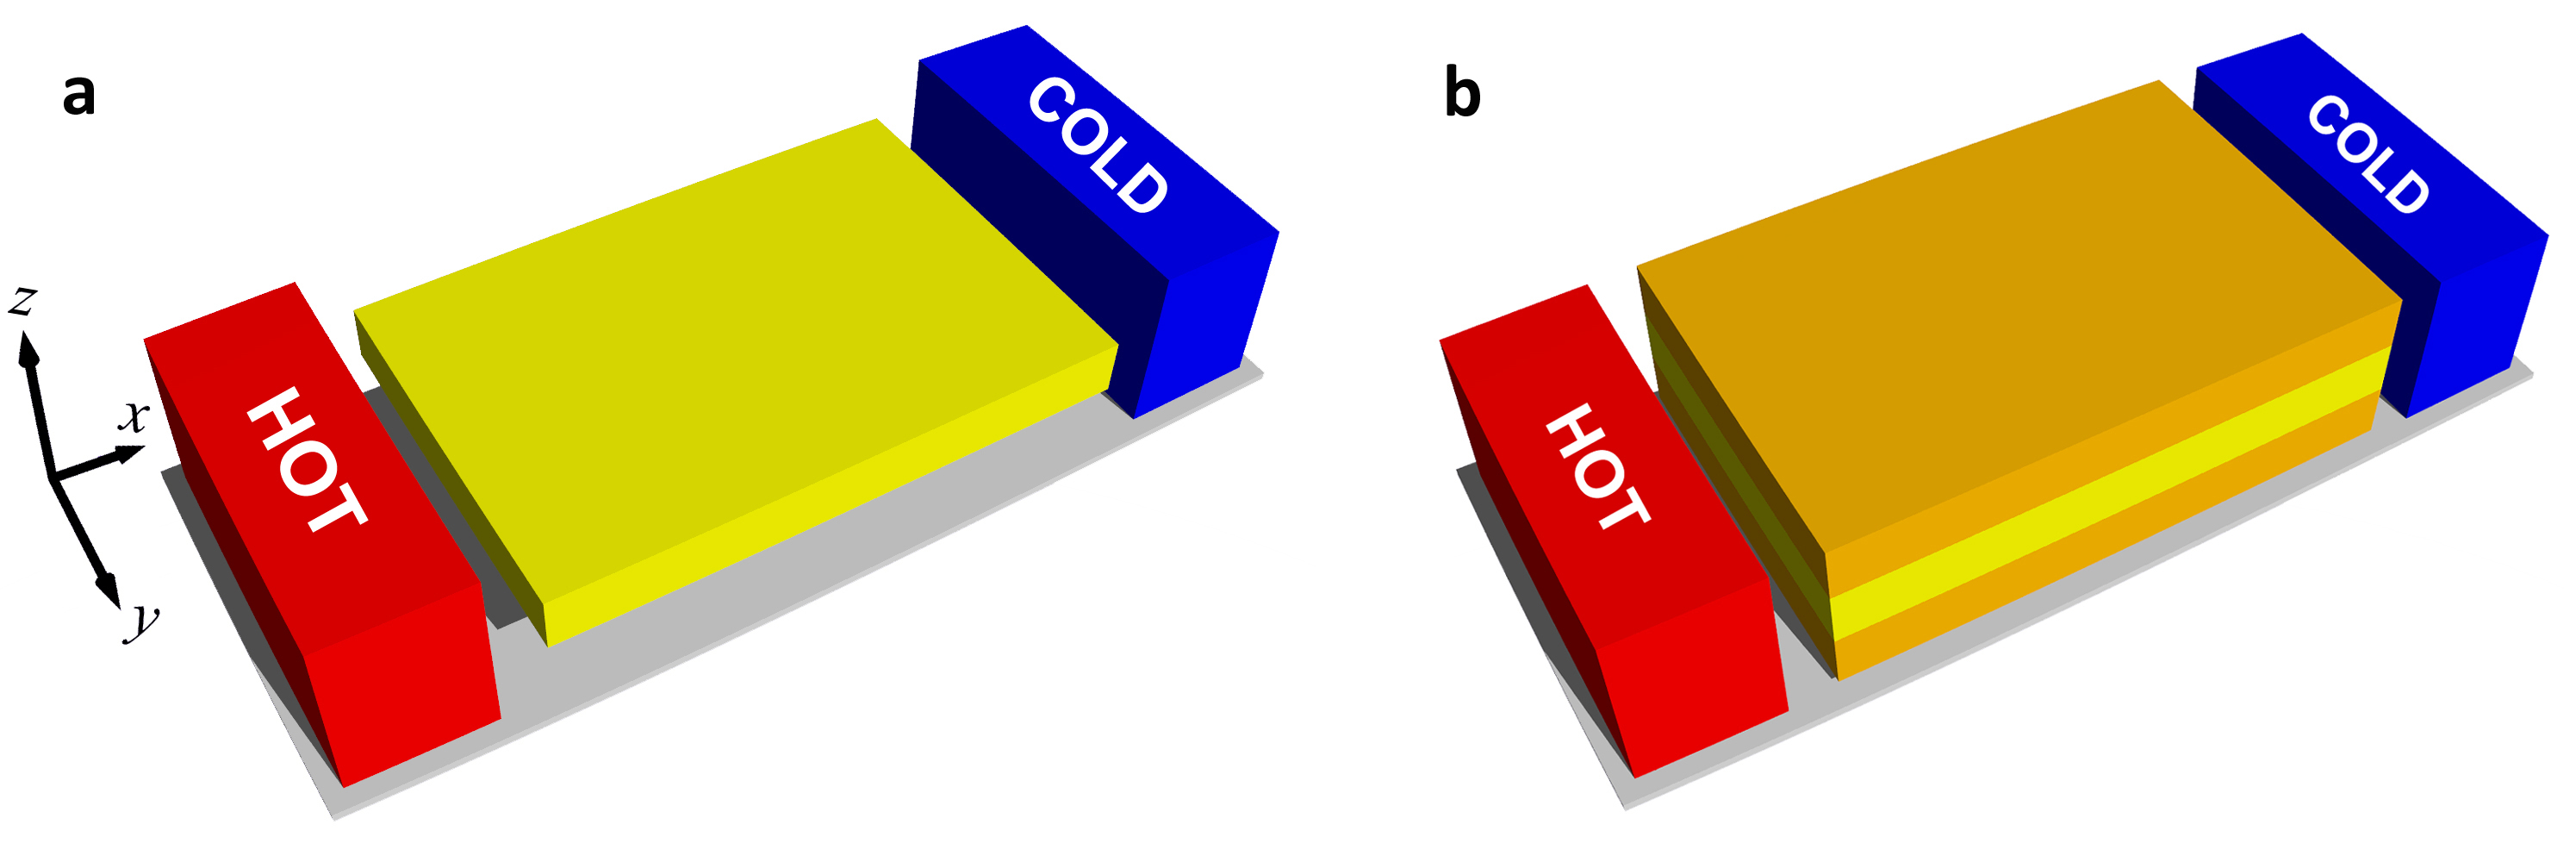
\includegraphics[width=1.0\textwidth]{figures/ch5/Fig1tl.jpg}
  \caption{Tri-layer superlattice nanostructure in (a). Schematic for a free-standing germanium thin film (yellow) in (b). By embedding the germanium thin film between silicon layers (orange) the thermal conductivity of the germanium film can be increased. The temperature gradient is applied to the whole structure in the $x$-direction.}
  \label{fig:ch5-tl}
\end{figure}

\subsection{Enhancement of Ge Layer Conductivity}
The calculated thermal conductivities of a germanium thin film in the tri-layer structure are shown in \Cref{fig:ch5-enh1} as a function of the thickness of the silicon cladding layer $t_{\text{Si}}$, where a significant enhancement in thermal conductivity of the germanium film over the free-standing counterpart is observed. Note that the dispersion relations in the [100] direction were used for these calculations, as reported in literature \cite{RN388}. We find that it is possible to nearly double the thermal conductivity (\textgreater90\% enhancement) of a 10 nm germanium thin-film by using two 1 \si{\micro}m thick silicon samples as cladding. Two cases for the specularities of the cladding-air interface are considered, \gls{p}$_{out}$ = 0 and 1, to cover all possibilities in terms of the quality of the silicon-air interfaces \cite{book_Ziman}. The germanium-silicon interface has roughness \gls{eta} = 0.1 nm. A germanium thin-film with given physical properties (surface roughness, correlation length, and thickness) without any cladding is used as the baseline measure for comparison. It is also observed that the larger the cladding thickness, the larger the increase in the thermal conductivity of the germanium thin film. This is because, for larger thicknesses of the silicon cladding layers, phonon scattering at the interfaces is reduced (see \Cref{chap:predictive}) and silicon phonon mean free paths are not shortened previously to their injection in germanium. Note that the enhancement of conductivity via injection of phonons is not unbounded with increasing cladding thickness, rather it begins to saturate as shown in \Cref{fig:ch5-enh1}(a). Clearly, increasing cladding thickness beyond the saturation limit is of no additional advantage from the perspective of enhancement, as the thermal conductivity contribution of phonons that can interact with the embedded layer has already been maximized. The specularity of the cladding-air interface is another factor that can influence the injection of phonons into the embedded layer. At the same cladding thickness, the observed enhancement of thermal conductivity in the embedded layer is higher for larger cladding-air surface specularities. This behavior is consistent since a more diffuse cladding shortens the phonon mean-free-paths, and therefore a larger thickness is required to improve the injection efficiency. Note that at sufficiently large cladding thicknesses, the impact of the quality of the silicon-air interface on germanium thermal conductivity enhancement begins to diminish and in the case of a bulk silicon cladding it would be expected that the enhancement is the same irrespective of the roughness of the cladding-air surface. Note that coherent modifications to the phonon dispersion relations can be neglected at room temperature owing to the choice of embedded layer thicknesses \cite{RN372}.
%Figure
\begin{figure}[hbtp]
  \centering 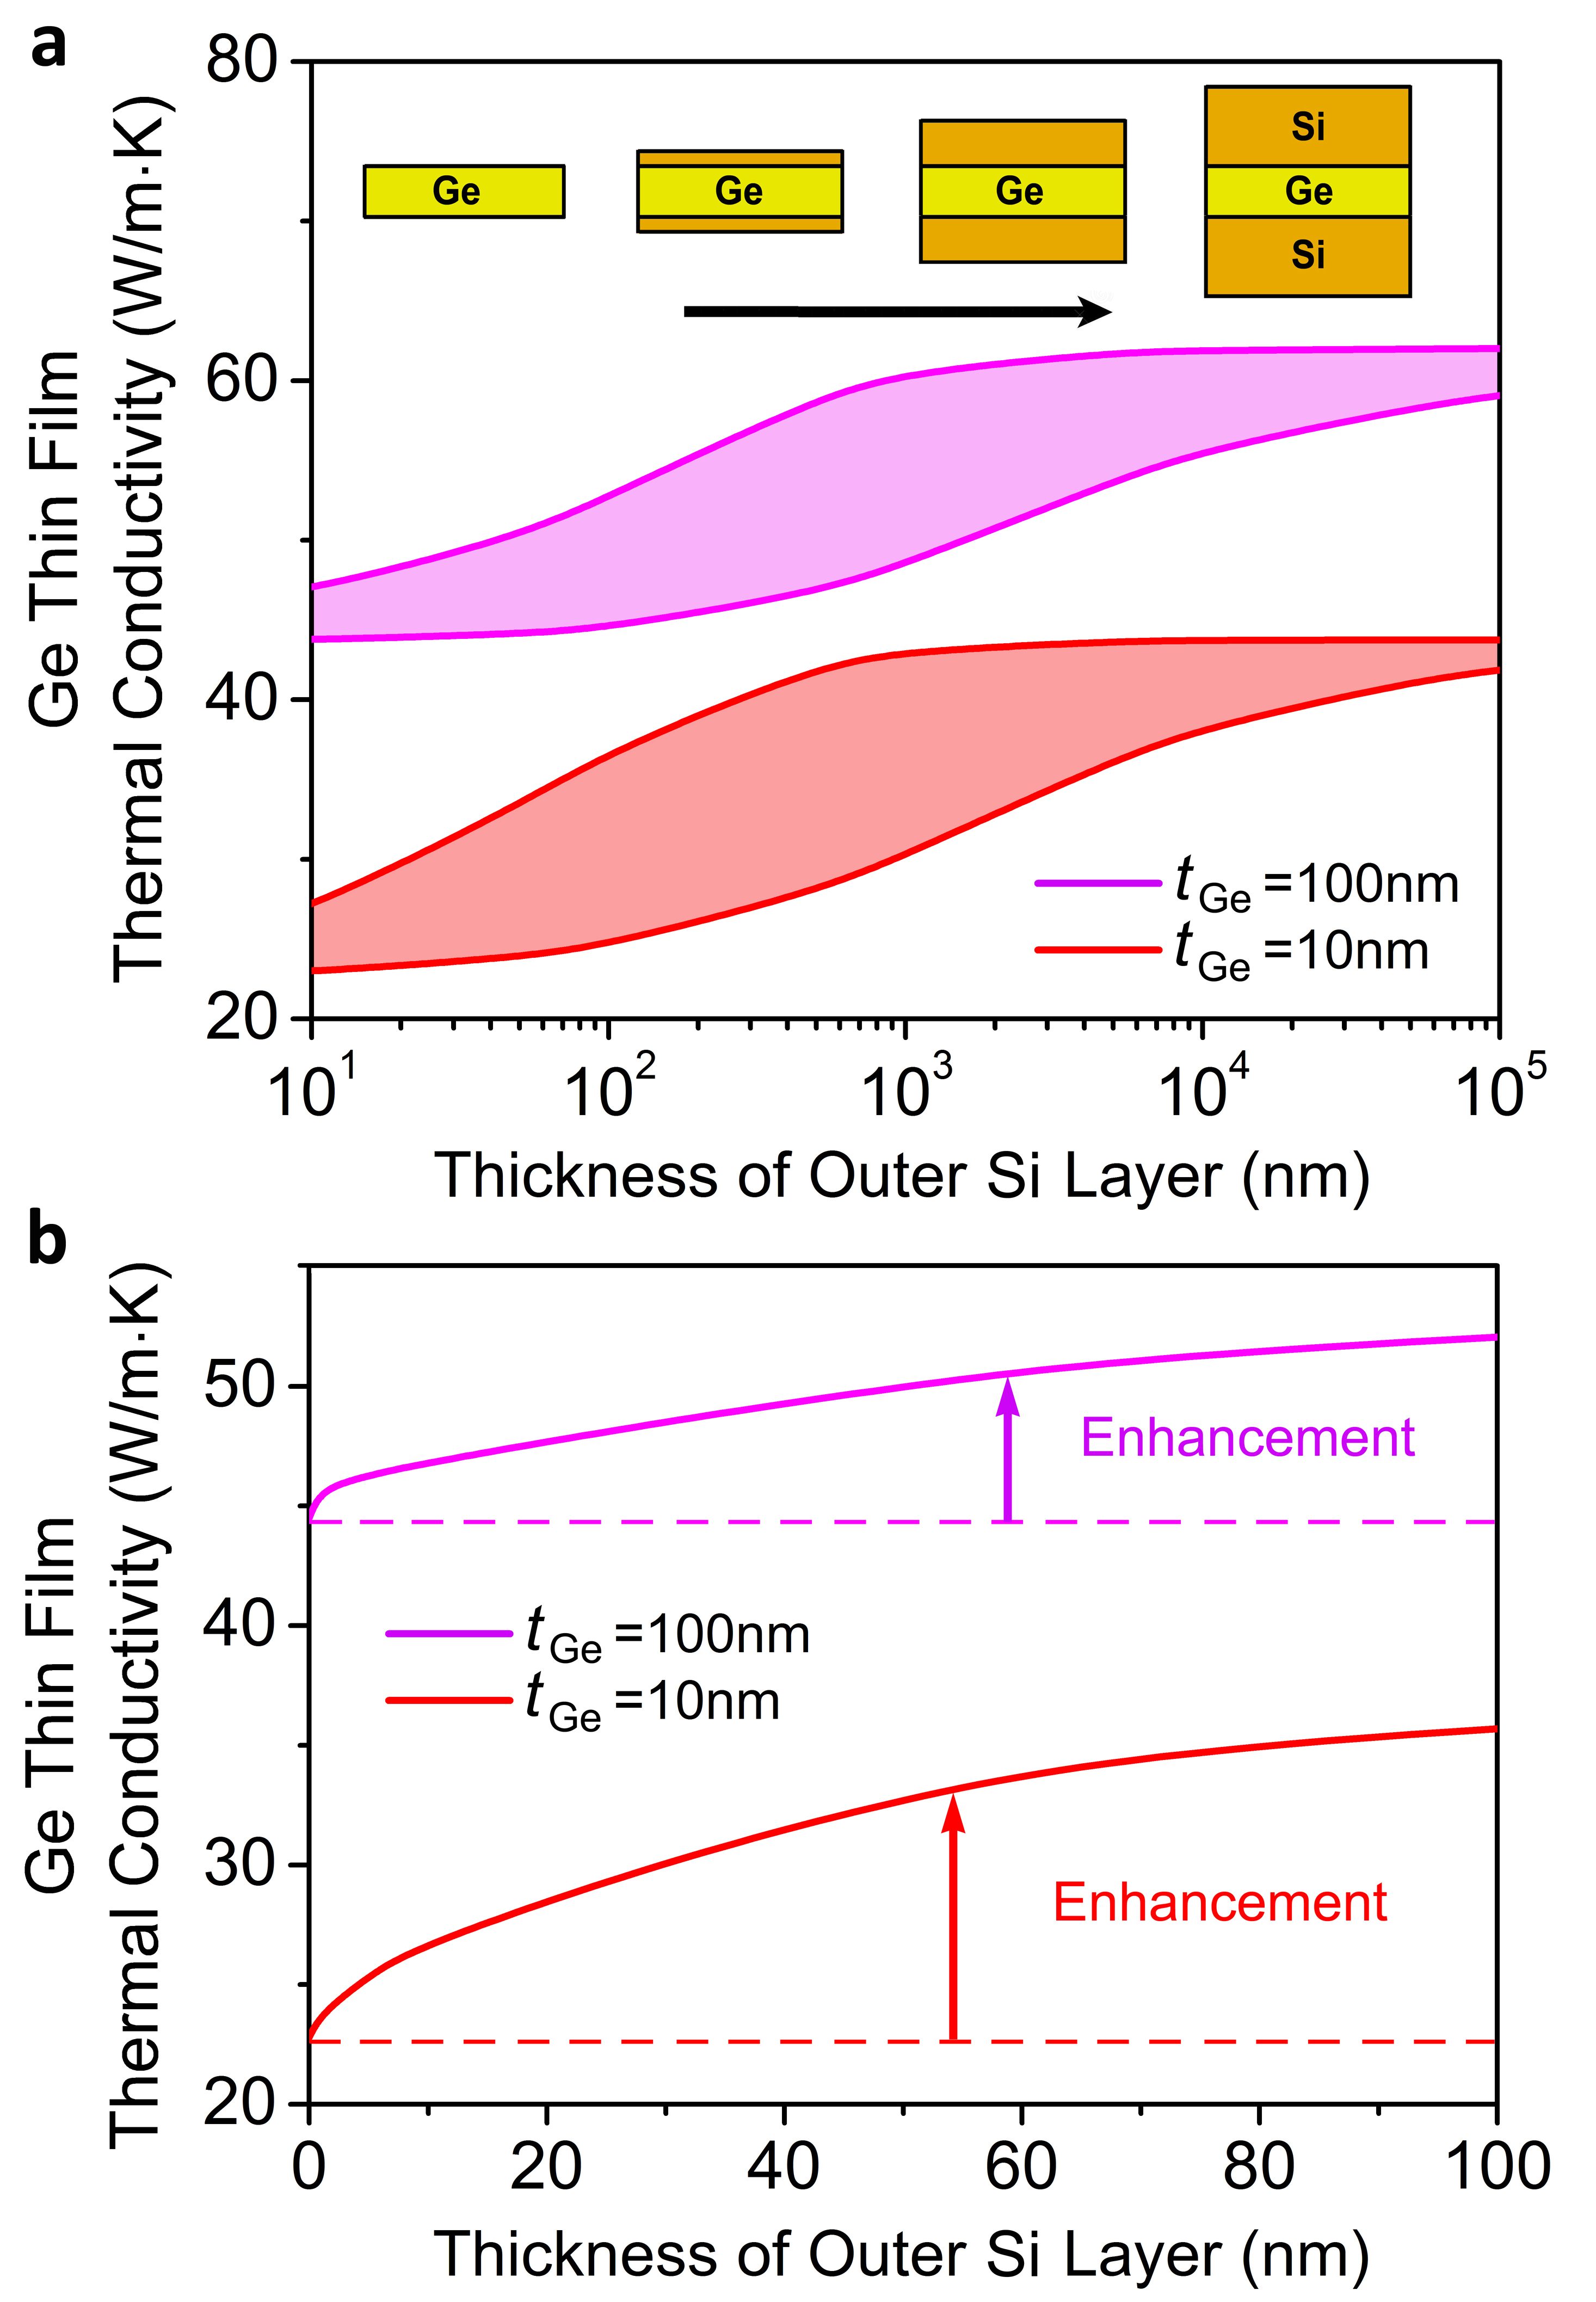
\includegraphics[width=0.80\textwidth]{figures/ch5/Fig1-enh.jpg}
  \caption{Increased thermal conductivity. (a) Colored areas show the enhancement in the thermal conductivity of a germanium thin film as a function of increasing thickness of the silicon cladding layer. The top and bottom lines correspond to silicon-air surface specularities \gls{p} = 1 and \gls{p} = 0, respectively, covering all possibilities in terms of surface roughness. The germanium-silicon interface has roughness \gls{eta} = 0.1 nm and correlation length \gls{cl} = 20\gls{eta}. (b) Enhanced thermal conductivity of an embedded germanium film (solid lines) with respect to a free-standing germanium thin film (dotted lines) having the same physical properties. The germanium-silicon interface has \gls{eta} = 0.1 nm, \gls{cl} = 20\gls{eta} while the silicon-air surface specularity is equal to one. The temperature gradient is in the plane of the films.}
    \label{fig:ch5-enh1}
\end{figure}
\par \Cref{fig:ch5-enh2} show the impact of silicon-germanium interface roughness on the increased thermal conductivity of the germanium film. Significant enhancements ($\sim$100\%) in thermal conductivities of the 10 nm embedded layer with roughness values in range of \gls{eta} = 0.1–0.4 nm can be achieved by using 1 \si{\micro}m silicon layers as cladding. Additionally, with increasing thickness of the embedded germanium layer, the maximum enhancement is reduced as the cladding is only able to inject phonons into a part of the thicker embedded germanium film. That is, the proportion of region in the germanium layer that is able to augment its local conductivity with the injected phonons from silicon decreases, leading to a smaller enhancement in thermal conductivity. Another interesting observation is that the thermal conductivity of a germanium thin-film can be enhanced beyond the bulk thermal conductivity of germanium at room temperature (60 W/m-K) using the described tri-layer architecture. However, it is important to note that the thermal conductivity enhancement in the embedded-layer occurs at the cost of reducing the thermal conductivity of the silicon cladding layer (as compared to a baseline silicon film of similar physical properties). In general, the reduction in thermal conductivity of the cladding layer would depend on structural properties including layer thicknesses and roughness. For a large ratio of cladding-to-embedded layer thickness, this reduction would be small since phonons from a small region near the interface would be able to couple across the interface. In simple words, the cladding layers allow for an enhancement of the thermal conductivity in the embedded layer by injecting phonons with sufficiently long mean-free-paths across the interface. 
%Figure
\begin{figure}[hbt]
  \centering 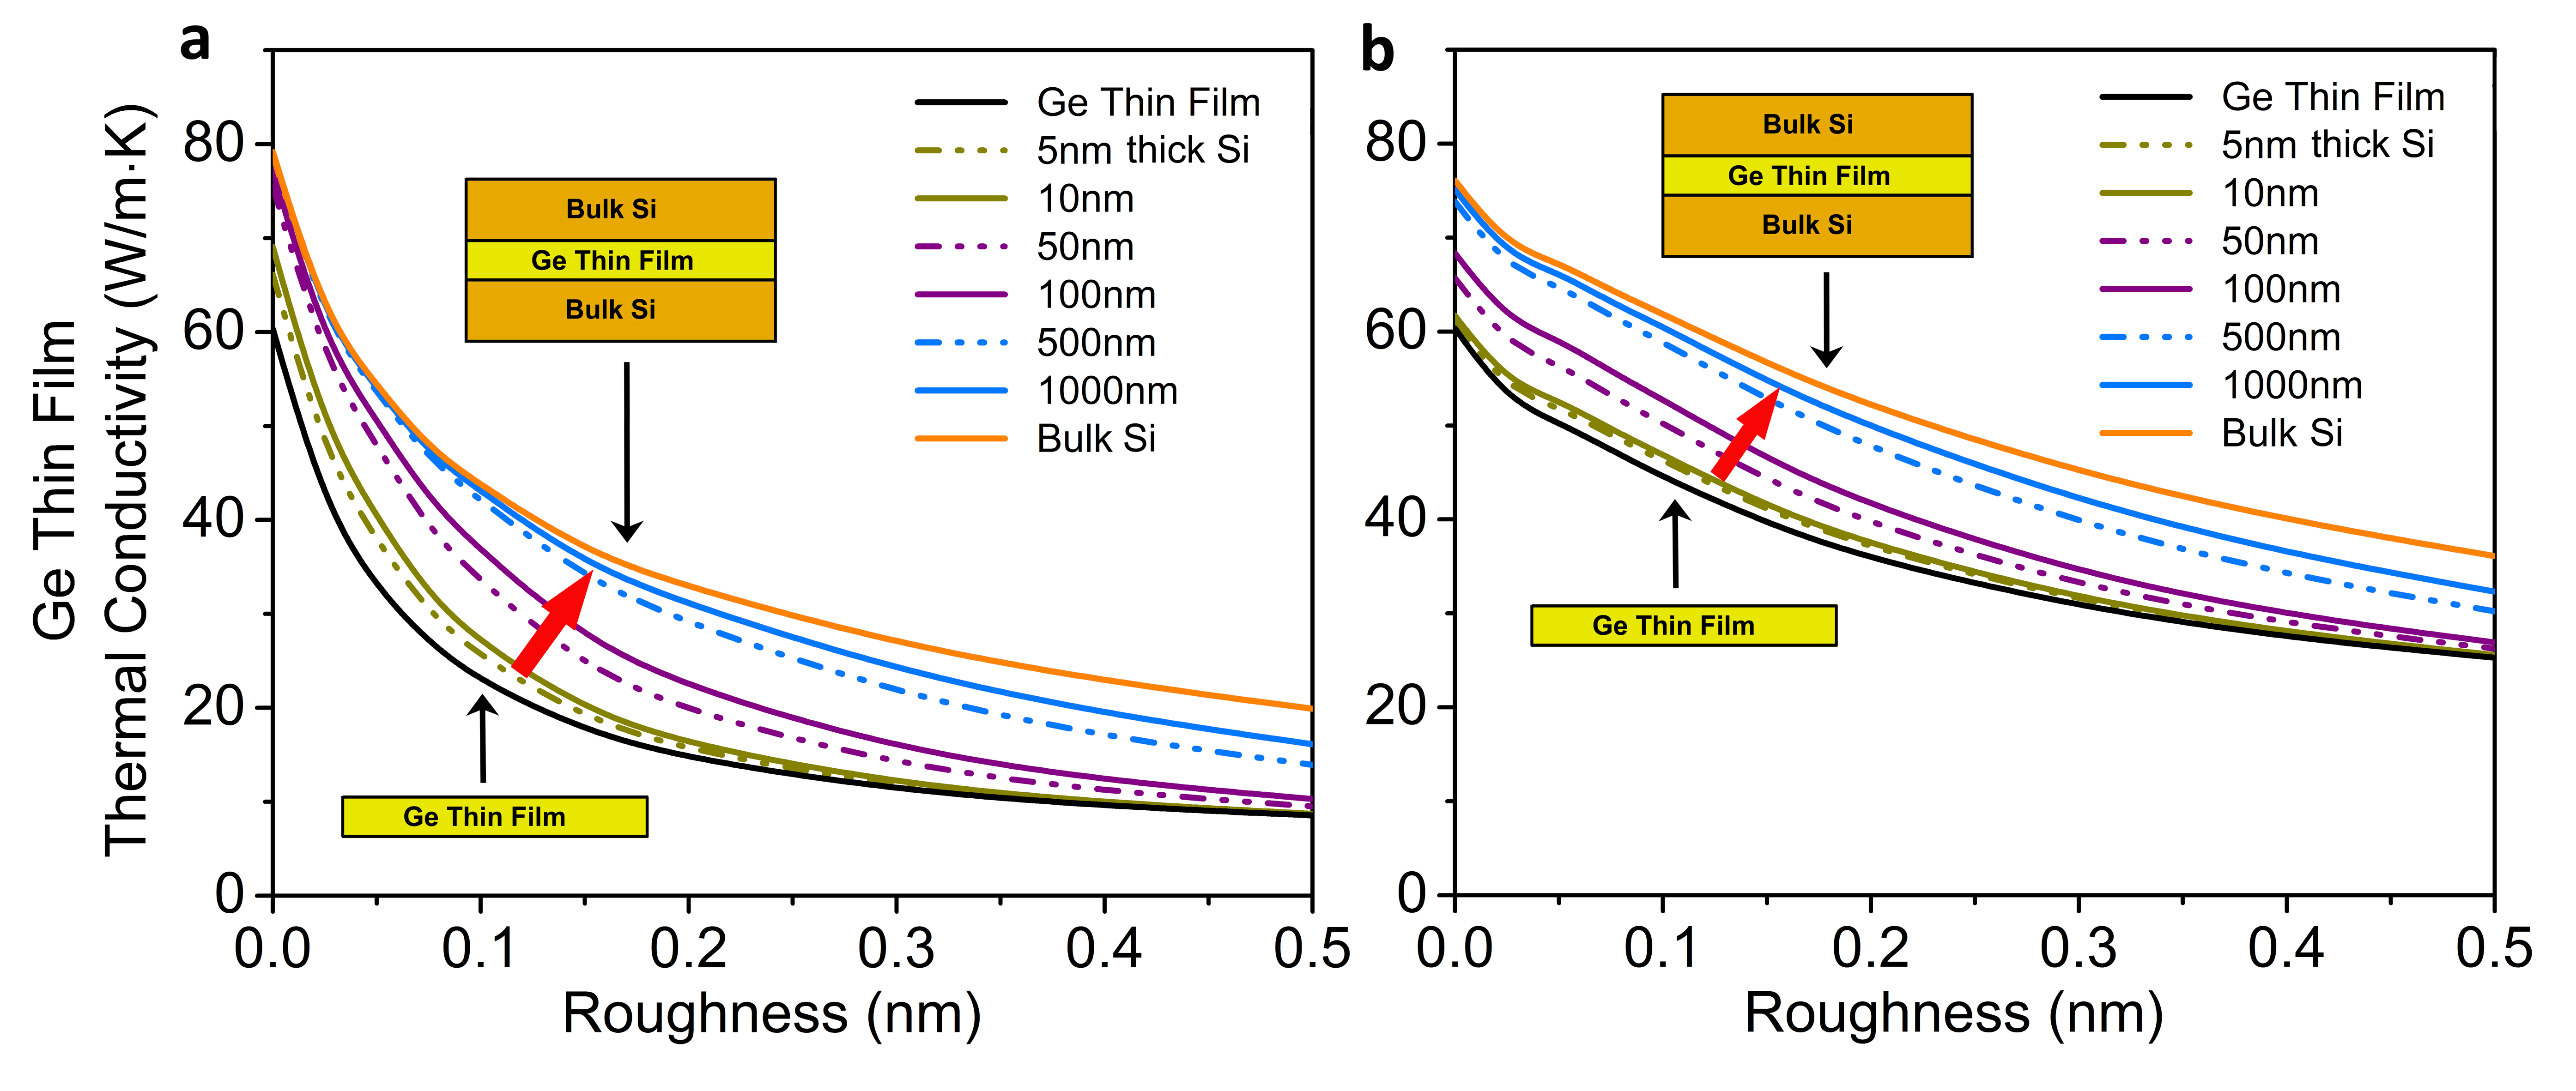
\includegraphics[width=1.0\textwidth]{figures/ch5/Fig2-enh.jpg}
  \caption{Enhanced heat conduction. Thermal conductivity increase for the embedded germanium film as a function of the silicon-germanium interface roughness. The germanium thin film thickness is (a) $t_{\text{Ge}}$ = 10 nm and (b) $t_{\text{Ge}}$ = 100 nm. Color lines correspond to different thicknesses of the silicon layers, increasing from no silicon layer to bulk silicon (indicated by red arrow). The enhancement in the thermal conductivity of the embedded germanium film, with respect to the free-standing germanium thin film with same properties, is observed for various surface roughnesses and silicon layer thicknesses.}
  \label{fig:ch5-enh2}
\end{figure}
%Figure
\begin{figure}[hbt]
  \centering 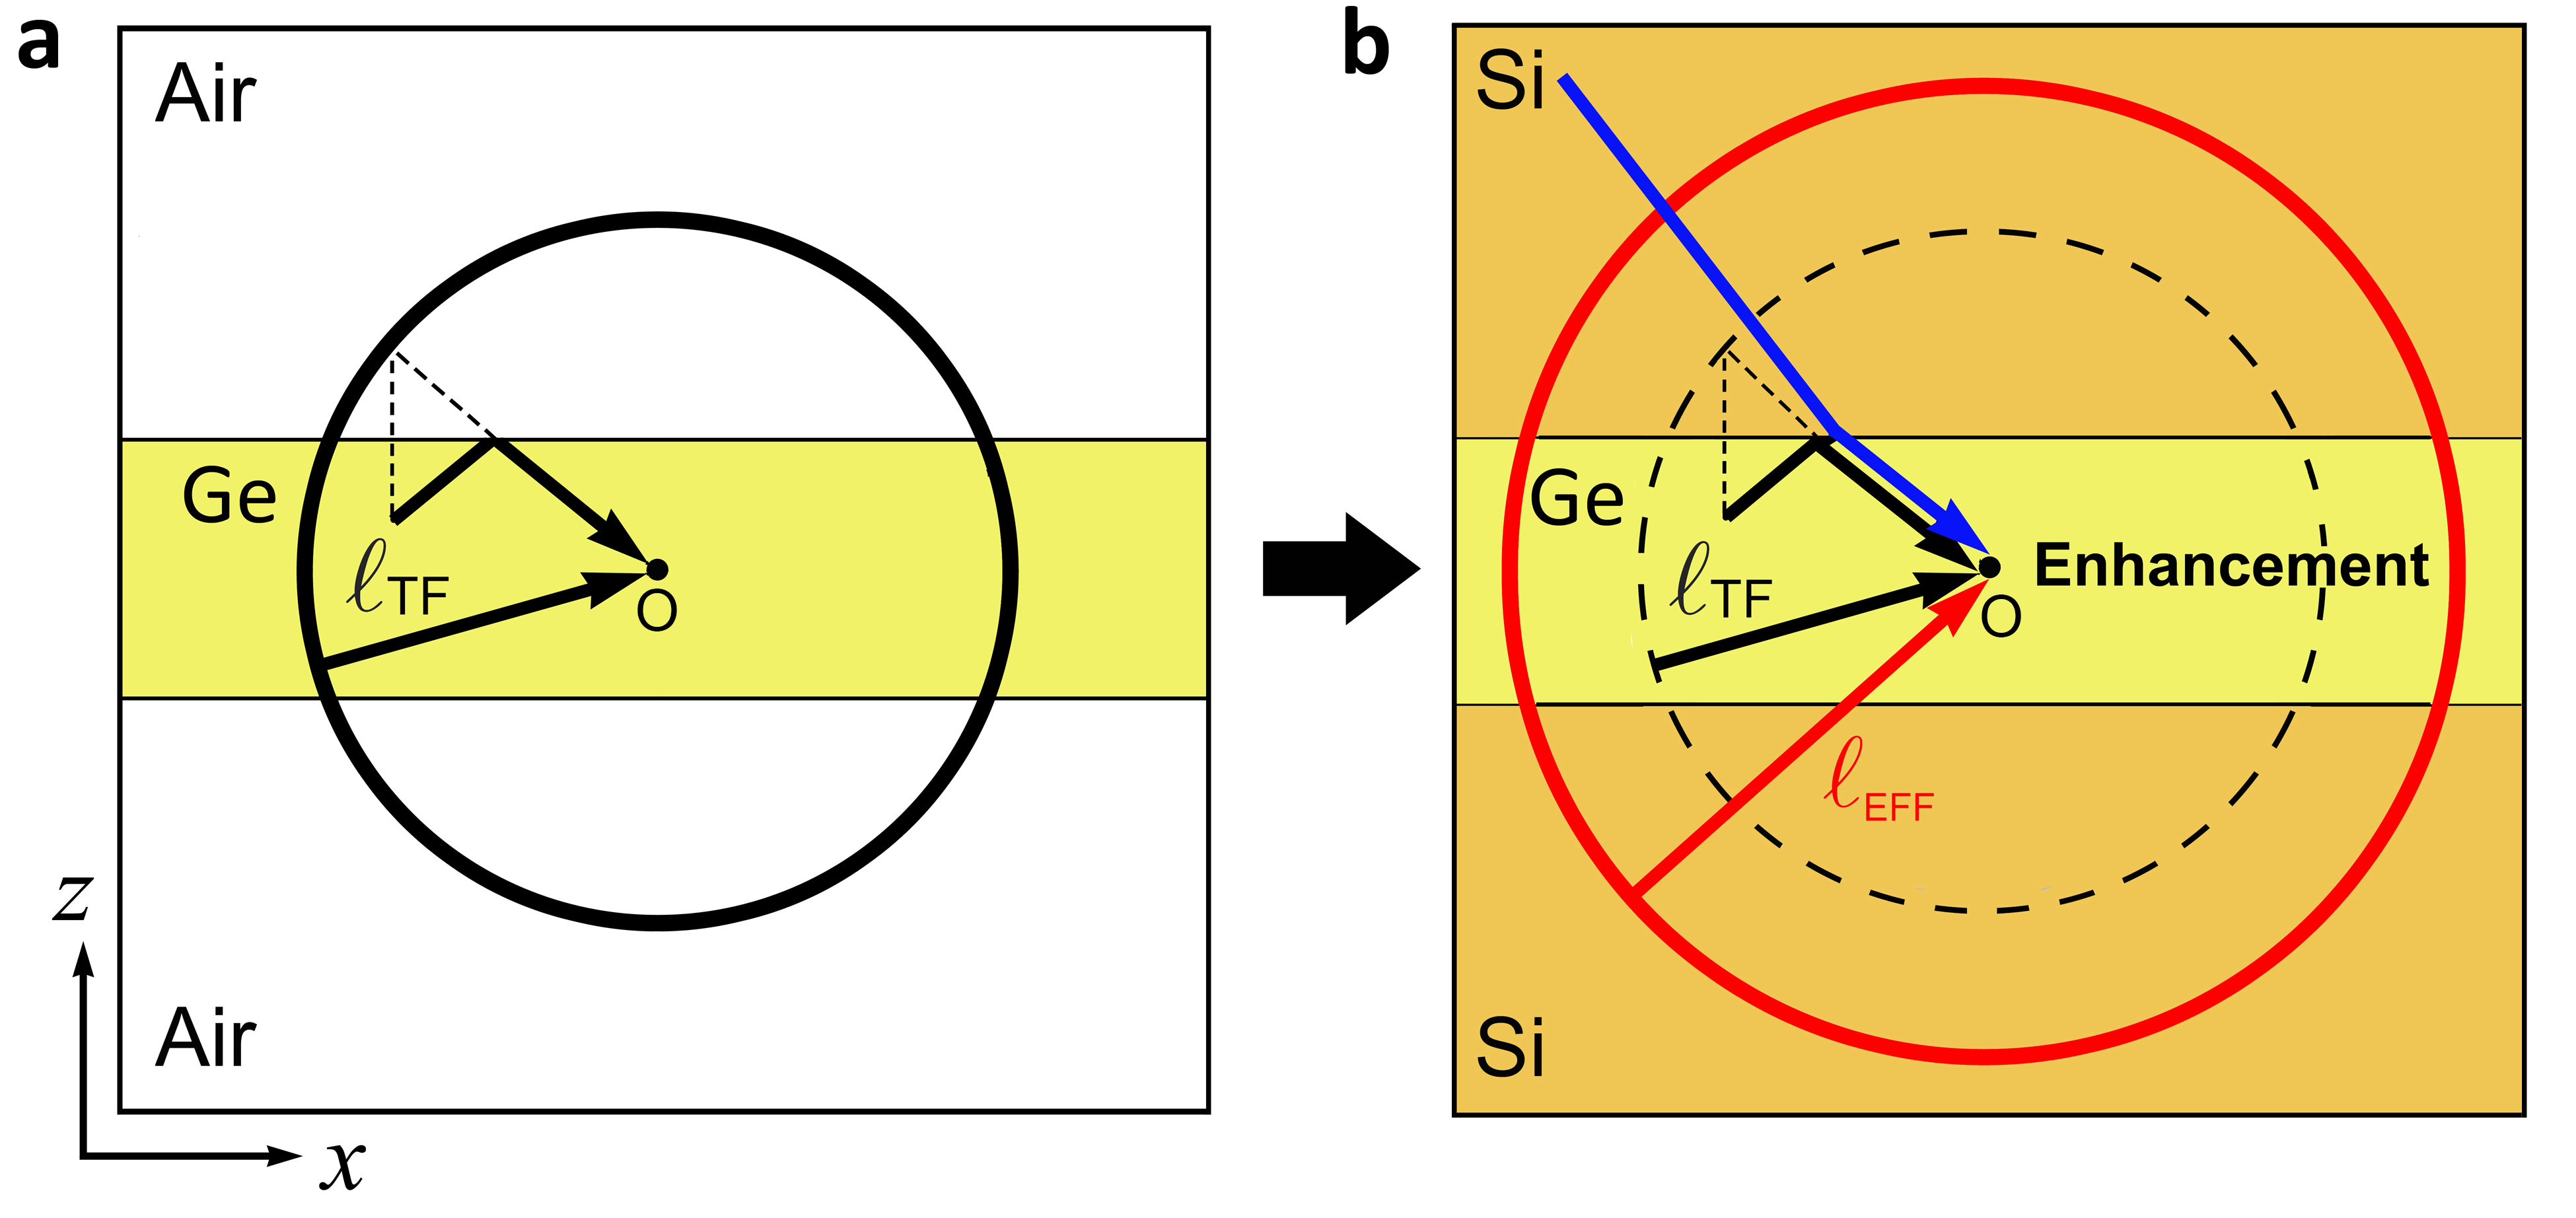
\includegraphics[width=0.90\textwidth]{figures/ch5/Fig3-enh.jpg}
  \caption{Phonon Injection. (a) Schematic for phonon contributions to the thermal conductivity of a germanium thin film under a temperature gradient along the $x$-direction. The thermal flux at point O is carried by phonons whose last collision was, on the average, at a distance of mean free path $\ell_{\text{TF}}$ away from O, as represented by the black circular line. For simplicity we neglect the angular dependence of $\ell_{\text{TF}}$. (b) When the germanium film is in contact with the silicon film, phonons from silicon can be injected into germanium (blue). These phonons had their last collision at a larger distance than those arriving from germanium. As a result, the effective mean free path $\ell_{\text{EFF}}$ is larger (red) and the thermal conductivity at point O is enhanced.}
    \label{fig:ch5-enh3}
\end{figure}
\par To further explain the origin of the thermal conductivity enhancement, we analyze the transport behavior of a well-established system of a “nanoparticle-in-alloy” bulk semiconductor \cite{RN98,RN29} and compare it with our nanostructured semiconductor. In a bulk structure, the thermal conductivity at a point O in real space is determined on an average by phonons coming from a spherical surface centered at that point with radius equaling the bulk mean free path in that semiconductor. Any changes to the semiconductor structure (such as addition of alloy atoms and nanoparticles) outside this “influence-sphere” can be considered to minimally affect the thermal conductivity at the point O. On the other hand, the inclusion of alloy atoms and nanoparticles within this influence-sphere will reduce the thermal conductivity by shortening the bulk phonon mean free paths, thereby reducing the effective radius of the influence-sphere. Analogous to the bulk case, in the case of a free standing thin-film [\Cref{fig:ch5-enh3}(a)], the thermal conductivity at a point O inside the film is determined on an average by phonons arriving from the surface of the influence sphere (see black circular line) given by the thin-film mean free path. We analyze the phonon trajectories and the impact of scattering on the effective phonon mean free paths for the germanium thin film and the tri-layer superlattice structure in \Cref{fig:ch5-enh3}. The addition of the silicon cladding layers to the germanium thin film [\Cref{fig:ch5-enh3}(b)] ensures that in addition to the phonons within the germanium layer, transmitted phonons from silicon that can couple across the interface and reach point O are able to enhance the thermal conductivity by increasing the effective mean free paths (red circle). This is because phonons arriving from silicon through transmission had their last collision on an average at a larger distance than those arriving from germanium. Consequently, we show that nanostructuring does not necessarily lead to a reduction in the germanium thermal conductivity, alternatively it can generate an enhancement of heat conduction.
\subsection{Reduction in Si Layer Conductivity} 
It is important to note that the increase of $\kappa_{\text{Ge}}$ should not be interpreted as an increase in the average thermal conductivity of the structure due to the addition of material (Si) with higher conductivity. In fact, here we show that the Si cladding layers reduce their thermal conductivities in the Si-Ge-Si tri-layer structure. We calculate the thermal conductivity $\kappa_{\text{Si}}$ of the outer cladding layers of Si in \Cref{fig:ch5-red1}. 
%Figure
\begin{sidewaysfigure}[hbtp]
  \centering 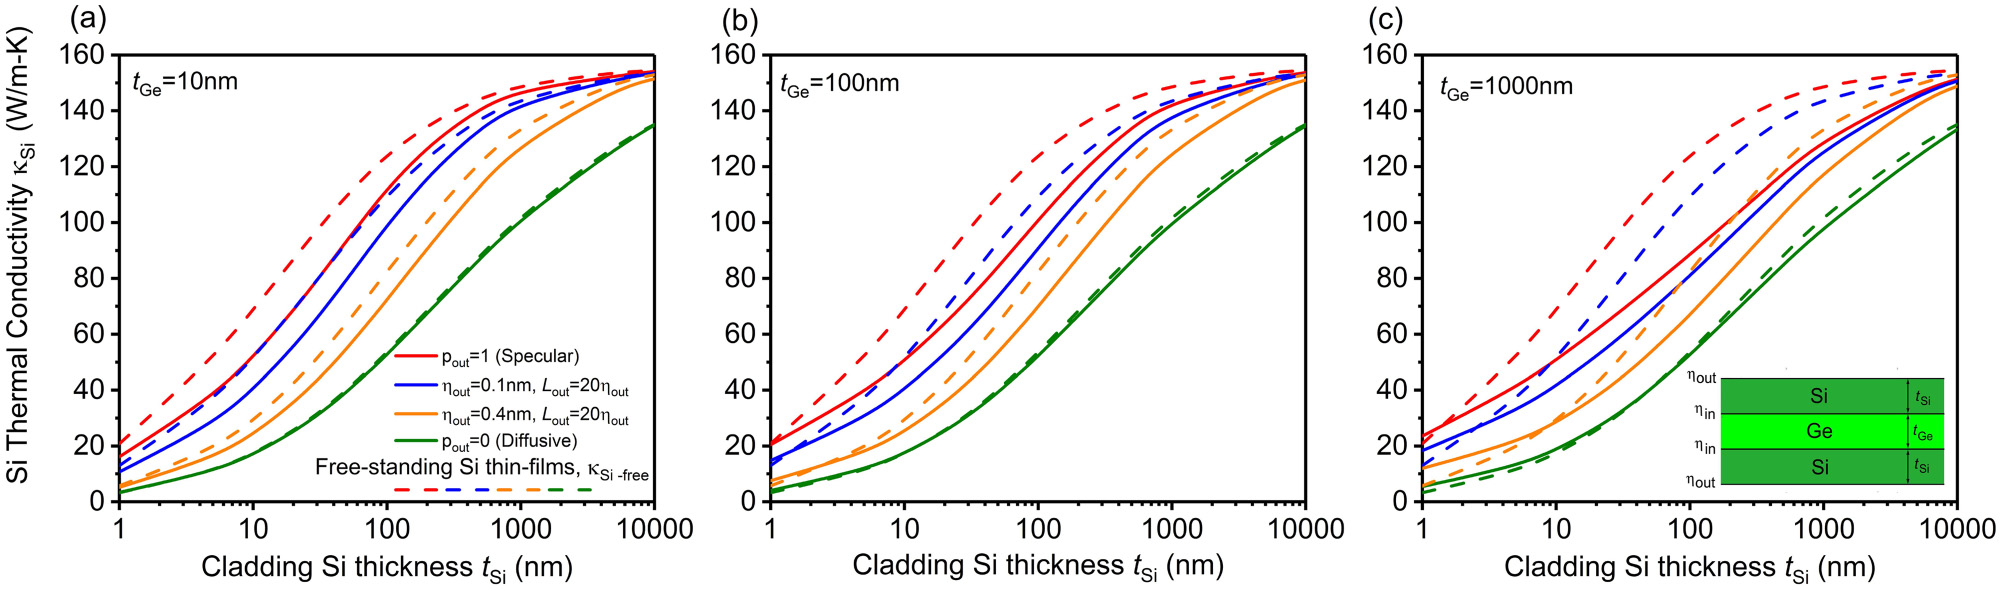
\includegraphics[width=1.0\textwidth]{figures/ch5/Fig1-red.jpg}
  \caption{Thermal conductivity of a cladding Si layer in a Si-Ge-Si architecture for different embedded layer thicknesses $t_{\text{Ge}}$ of (a) 10 nm, (b) 100 nm, and (c) 1000 nm. The inner roughness $\eta_{in}$ is 0.1 nm. The plots show the dependence of the thermal conductivity $\kappa_{\text{Si}}$ on cladding layer thickness $t_{\text{Si}}$ and outer Si-air interface conditions. The corresponding Si free-standing thin-film conductivity $\kappa_{\text{Si-free}}$ is shown for reference with dotted lines.}
    \label{fig:ch5-red1}
\end{sidewaysfigure}
In this system, the outer interface is defined as the interface between the outer Si layer and air and the inner interface is between Ge and Si layers. Note that the surface conditions of the baseline free-standing Si film are the same as the cladding Si layer in the tri-layer structure, i.e., roughness of the Ge-Si interface on one side and the roughness of the Si-air interface on the other, in order to obtain a comparison with same surface conditions and independently study the effects of phonon coupling between layers. In general, we find that $\kappa_{\text{Si}}$ falls below its corresponding free-standing thin-film value $\kappa_{\text{Si-free}}$. This result shows that the Si layer acts as a “net injector” of phonons into the Ge layer thereby reducing its own conductivity. We find that the reduction in $\kappa_{\text{Si}}$ in comparison to $\kappa_{\text{Si-free}}$ is larger for (a) thick Ge embedded layers and (b) smooth outer surfaces. A larger reduction in $\kappa_{\text{Si}}$ from $\kappa_{\text{Si-free}}$ for larger $t_{\text{Ge}}$ is obtained since more injected phonons travel in the Ge layer reducing the mean-free-paths below the freestanding values. For small $t_{\text{Ge}}$, phonons from one Si layer can travel across the Ge layer into the other Si layer (which possesses higher transport properties) thereby reducing their thermal conductivity to a lesser degree. In the case of a fully diffusive outer surface, the reduction of $\kappa_{\text{Si}}$ from $\kappa_{\text{Si-free}}$ is small since those phonons in the Si layer that interact with the diffusive interface are prevented from being reflected and thus being injected into the Ge layer. Thus, a strong shortening of phonon mean-free-paths in the Si layer effectively reduces the injection of phonons into the embedded layer. We note that the increase in $\kappa_{\text{Si}}$ with increasing thickness $t_{\text{Si}}$ is a consequence of the reduction of phonon surface scattering in the quasi-ballistic regime and not due to phonon coupling effects and is thus observed for both free-standing Si thin-films (dashed lines) and Si-layer in the tri-layer architecture (solid lines). To understand the role played by inner interface properties, we increase the inner Ge-Si roughness to $\eta_{in}$ = 0.4 nm as shown in [\Cref{fig:ch5-red2}]. The increased $\eta_{in}$ lowers the coupling of phonons between cladding and embedded layers as more phonons get diffusively scattered at the rougher interface (\Cref{eq:bezak_transmission}). The reduced phonon coupling for $\eta_{in}$ = 0.4 nm is manifested as a lesser reduction of $\kappa_{\text{Si}}$ with respect to $\kappa_{\text{Si-free}}$ [\Cref{fig:ch5-red2}] in comparison to $\eta_{in}$ = 0.1 nm [\Cref{fig:ch5-red1}]. For very large surface roughnesses $\eta_{in}$ (e.g., $p_{in}$ = 0), all the layers can be treated as decoupled from each other and, in that case, all phonon coupling effects on thermal transport would be negligible. 
%Figure
\begin{sidewaysfigure}[hbtp]
  \centering 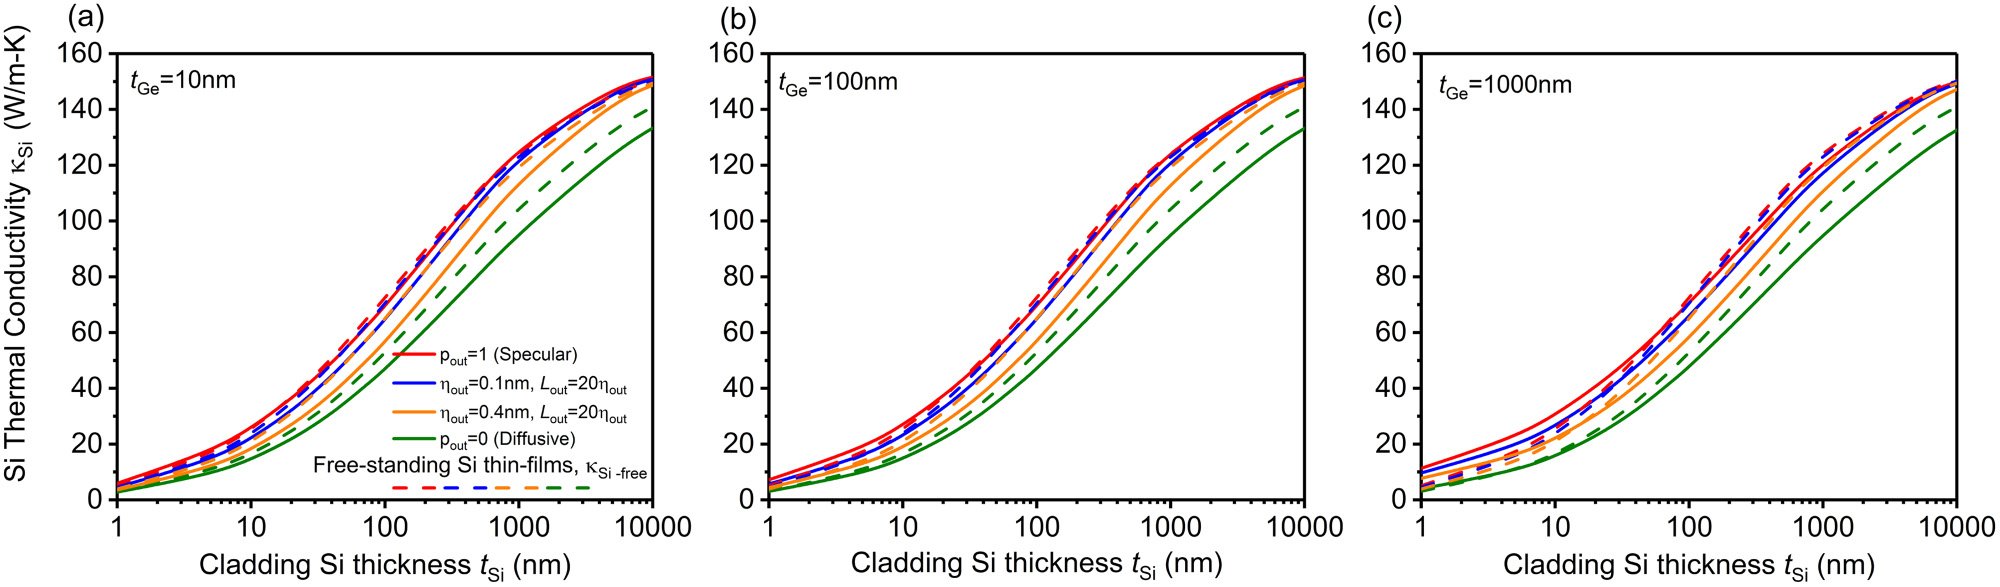
\includegraphics[width=1.0\textwidth]{figures/ch5/Fig2-red.jpg}
  \caption{Thermal conductivity of embedded Si layer $\kappa_{\text{Si}}$ in a Si-Ge-Si architecture with inner roughness $\eta_{in}$ = 0.4 nm as a function of cladding layer thickness $t_{\text{Si}}$. The thickness of the embedded layer $t_{\text{Ge}}$ is increased from (a) 10 nm, (b) 100 nm to (c) 1 \si{\micro}m, and four outer surface conditions are considered -- specular, $\eta_{out}$ = 0.1 nm, $\eta_{out}$ = 0.4 nm, and diffuse.}
    \label{fig:ch5-red2}
\end{sidewaysfigure}

\subsection{Si-Ge Bi-layers}
 We have focused our previous analysis on tri-layer structures made of Si and Ge with varying layer spacing to analyze the coupling of phonons between the layers and understand the impact on thermal conductivity modulations in each layer. Since the mechanism of phonon coupling is independent of the number of layers, the analysis can be extended to any arbitrary $n$-layered structure. We note that structures with $n$ = 2, i.e., bi-layers are a common experimentally grown structure, and the experimental measurement of each layer’s thermal conductivity \cite{RN189,RN126} could potentially be easier to achieve as compared to a tri-layer system. With the motivation for guiding future experiments, we briefly analyze the thermal conductivity modulations in a bi-layer system of Si and Ge with thickness of each layer given as $t_{\text{Si}}$ and $t_{\text{Ge}}$. We note that for a Si-Ge bi-layer, the system of equations to evaluate deviation functions \gls{g}$_i$ for layer-1 (Si) and layer-2 (Ge) can be easily extended to account for the changed boundary conditions from the tri-layer system discussed earlier. In a Si-Ge bi-layer system, three interfaces exist--the top Si-air interface, the Si-Ge interface, and the bottom Ge-air interface. For simplicity, we assume identical interfacial conditions for both the outer Si-air and Ge-air interfaces. Thermal conductivity modulations in three structures with different thicknesses of silicon and germanium (i) $t_{\text{Si}}$= $t_{\text{Ge}}$ = 10 nm, (ii) $t_{\text{Si}}$ = 100 nm, $t_{\text{Ge}}$ = 10 nm, and (iii) $t_{\text{Si}}$= $t_{\text{Ge}}$ = 100 nm are considered to elucidate the impact of phonon coupling. \Cref{fig:ch5-bilayer} shows that analogous to tri-layer structures, silicon thermal conductivity $\kappa_{\text{Si}}$ is reduced below its free standing thin-film value $\kappa_{\text{Si}}$-free when phonons originating in Si are injected into Ge causing a corresponding enhancement in $\kappa_{\text{Ge}}$. The impact of phonon coupling on thermal conductivity modulations in each layer is stronger when the inner surface is smoother as indicated by the larger differences in layer thermal conductivities in top panels in contrast to bottom-panels of \Cref{fig:ch5-bilayer} from their respective free-standing values. The enhancement in $\kappa_{\text{Ge}}$ is higher when silicon layer thickness $t_{\text{Si}}$ is large, while the reduction in $\kappa_{\text{Si}}$ is higher when germanium layer thickness $t_{\text{Ge}}$ is larger, clearly indicating the reciprocity in phonon injection process as was observed in tri-layer architectures. These findings would be useful for future experimental investigations into phonon coupling.
 %Figure
\begin{figure}[hbt]
  \centering \includegraphics[width=1.0\textwidth]{figures/ch5/Fig4.jpg}
  \caption{Thermal conductivity of layers of silicon $\kappa_{\text{Si}}$ (solid blue square) and germanium $\kappa_{\text{Ge}}$ (solid red circle) in bi-layer structures with different silicon and germanium layer thicknesses: [(a), (d)] $t_{\text{Si}}$= $t_{\text{Ge}}$= 10 nm, [(b), (e)] $t_{\text{Si}}$= 100 nm, $t_{\text{Ge}}$ = 10 nm, and [(c), (f)] $t_{\text{Si}}$ = $t_{\text{Ge}}$ = 100 nm. Top panels correspond to inner roughness $\eta_{in}$ = 0.1 nm and bottom panels to $\eta_{in}$ = 0.4 nm. Four different outer surface conditions are shown on the $x$-axis in each panel -- specular, $\eta_{\text{Si-air}}$ = $\eta_{\text{Ge-air}}$  = 0.1 nm, $\eta_{\text{Si-air}}$ = $\eta_{\text{Ge-air}}$ = 0.4 nm, and diffuse. Open symbols represent the corresponding free-standing thin-film conductivity $\kappa_{\text{Si-free}}$ (blue) and $\kappa_{\text{Ge-free}}$ (red).}
    \label{fig:ch5-bilayer}
 \end{figure}
 %
\subsection{Films-on-substrate}
We also consider a baseline physical system consisting of a thin-film of material A on top of a substrate of material B. Our choice of A and B is motivated from optoelectronic applications such as photo-detectors where configurations based on Si, Ge, GaAs and AlGaAs semiconductors are found ubiquitously \cite{book_rogalski_infrared,RN387,ownKK1}. We focus on studying the influence of this semi-infinite substrate on the thermal conductivity modulation in the film-on-substrate (FOS) system [\Cref{fig:ch5-fos1}] and contrast the unique behavior with free-standing isolated thin films.
%Figure
\begin{figure}[hbt]
  \centering 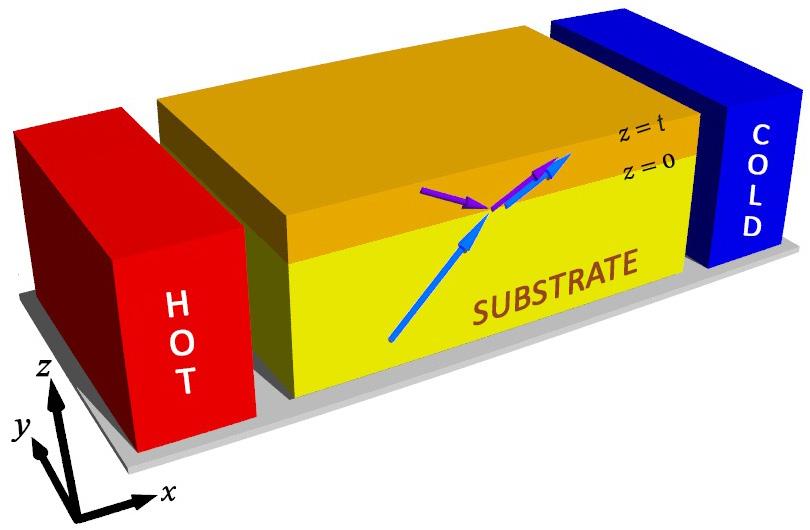
\includegraphics[width=0.75\textwidth]{figures/ch5/Fig5-fos1.jpg}
  \caption{Schematic of a film-on-substrate (FOS) architecture where the film is shown in orange and the substrate in yellow. Arrows represent phonons originating at the film and the substrate and contributing to film phonon transport after reflection and transmission (inter-layer coupling).}
    \label{fig:ch5-fos1}
 \end{figure}
 %Figure
\begin{figure}[hbt]
  \centering 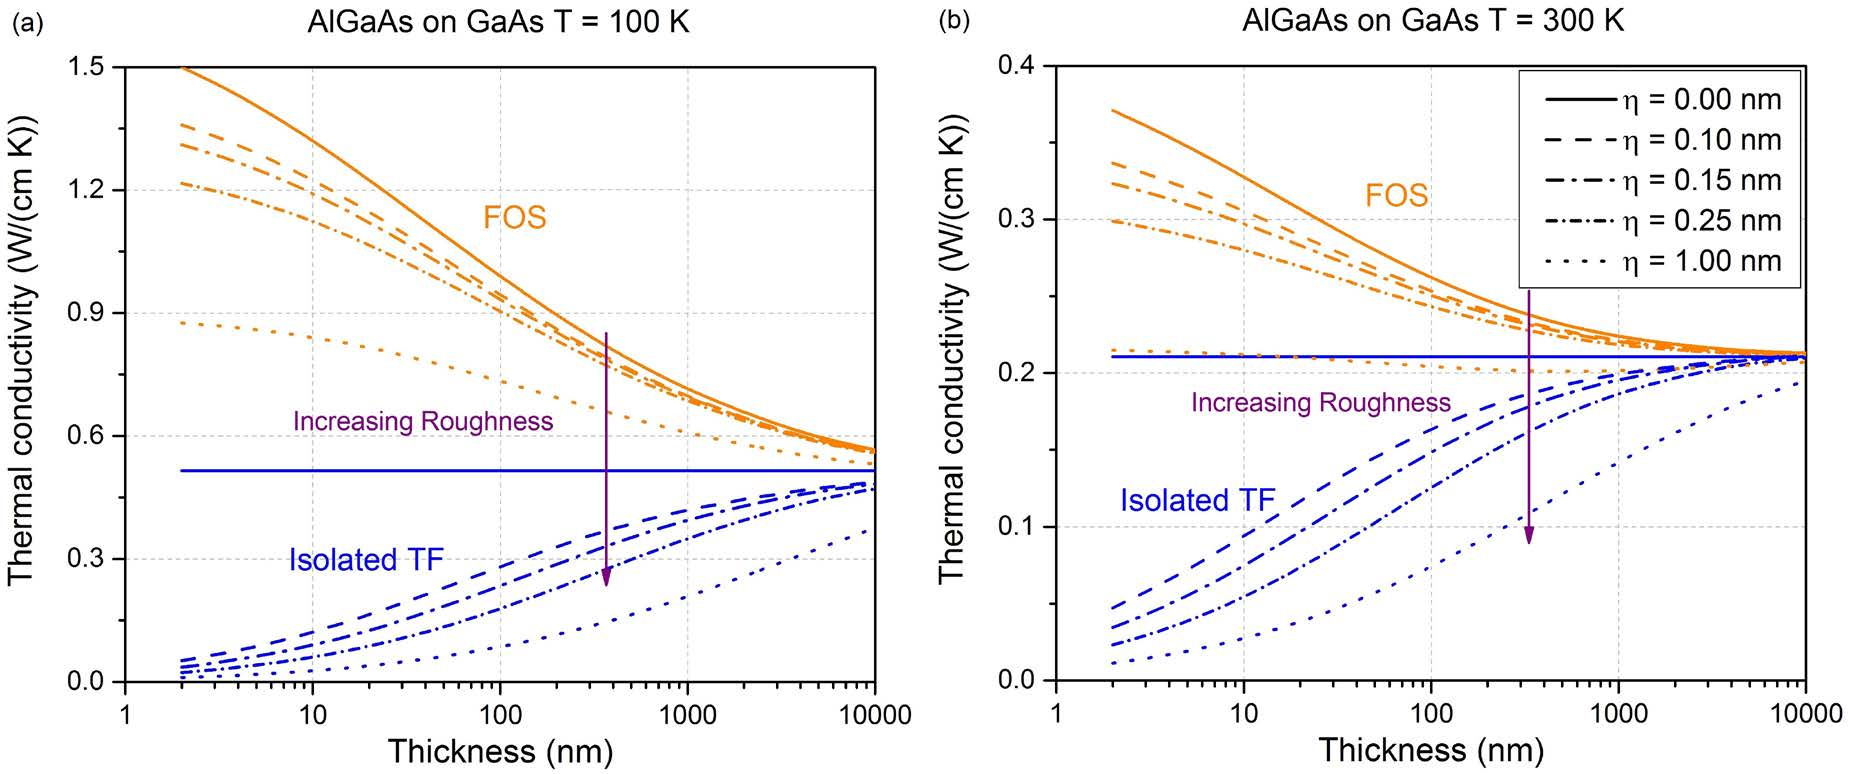
\includegraphics[width=1.0\textwidth]{figures/ch5/Fig5-fos2.jpg}
  \caption{Thermal conductivity of an \algas{0.10}{0.90} thin film grown on GaAs substrate in FOS architecture (orange lines) and an isolated free-standing \algas{0.10}{0.90} thin film (blue lines) for different interfacial roughnesses at temperatures (a) \gls{T} = 100 K and (b) \gls{T} = 300 K. The vertical arrow denotes the direction of increasing roughness. Blue horizontal line corresponds to the bulk thermal conductivity of \algas{0.10}{0.90}.}
    \label{fig:ch5-fos2}
 \end{figure}
 \par We show in \Cref{fig:ch5-fos2} the predicted thermal conduction variation of a ternary alloy \algas{0.10}{0.90} thin film atop a GaAs substrate for the case of equal inner and outer surface conditions, while varying the thickness of the \algas{0.10}{0.90} thin film. Our calculations show that the thermal conductivity $\kappa$ of the thin film in the FOS architecture increases with decreasing thickness, which is exactly the opposite of the conventional free-standing calculations \cite{RN204,ownTF} which predict that it decreases. Specifically, we found that the thermal conductivity of a thin-film in a FOS structure can be larger than the bulk thermal conductivity (horizontal blue line) as well as that of an isolated, free-standing film of the same material with similar structural properties. The observed enhancement in the thermal conductivity ($\Delta\kappa$) of the \algas{0.10}{0.90} film is attributed to phonon injection from the substrate \cite{ownCoupling1}. For certain surface conditions, interfacial coupling between the thin film and the substrate allow phonons to be exchanged between the two media. In the FOS case, the phonon mean-free-paths of the substrate material are larger than their corresponding thin-film phonon mean-free-path. Since the local thermal conductivity at a point inside the thin film is determined by the effective mean-free-path of phonons reaching that point, the local thermal conductivity of the thin-film in the FOS structure is enhanced beyond the isolated thin-film value due to an injection of larger mean-free-path phonons from the substrate, which leads to a larger effective mean-free-path for phonons in the thin-film. For the case when phonons in the thin film have larger mean-free-paths compared to the substrate, the thermal conductivity of the FOS would be smaller than the corresponding isolated thin-film. It is noteworthy that the thermal conductivity $\kappa$ of the film can be enhanced beyond the \algas{0.10}{0.90} bulk conductivity value. We denote this enhancement of thermal conduction beyond the bulk conductivity values by $\Delta\kappa_{\text{bulk}}$ whereas we denote the enhancement beyond isolated thin film conductivity values as $\Delta\kappa_{\text{iso}}$. We remark that we observe an increasing $\Delta\kappa_{\text{bulk}}$ with reducing thickness of thin film for a wide range of interfacial roughnesses. This finding can have profound consequences since achieving enhanced thermal conduction is a key component of enabling heat dissipation from hot spots in optoelectronic and microelectronic applications. The facilitation of effective heat dissipation in nanostructures can further promote miniaturization and efficient power consumption in devices. We observe this trend of enhancement beyond bulk conductivity $\Delta\kappa_{\text{bulk}}$ to be significant even at \gls{T} = 300 K, which shows that devices will be competent for room temperature operation as well. We note that, the unconventional increase in the thermal conductivity of the thin film in the FOS architecture with decreasing thickness can be understood in light of recognizing the role of interfacial scattering and film thickness. For small roughnesses, we have low diffusive interfacial scattering, and due to the low acoustic impedance mismatch between \algas{0.10}{0.90} and GaAs there is a strong inter-layer phonon coupling in the system. With decreasing film thickness, the volume fraction in the film in which there is an enhancement of thermal conductivity arising from inter-layer phonon coupling increases because phonons being injected from GaAs, which have finite mean-free-path, are allowed to influence a larger film proportion. As a result, the thermal conductivity $\kappa$ of the film increases with decreasing thickness for $\eta$ = 0, 0.10, 0.15 and 0.25 nm because the enhancement by phonon coupling is larger than the decrease by diffuse interface scattering. On the other hand, for the isolated free-standing thin film, we observe a reduction in thermal conductivity with decreasing thickness, which is due to conventional boundary scattering. Note that in this case there is no inter-layer phonon coupling and therefore there are no physical mechanisms to observe an increase in heat conduction. Significantly, we found that the different physical mechanisms behind thermal transport in isolated and FOS films can lead to opposite thermal conductivity behaviors when the film thickness is reduced. We note that we investigate the thermal conductivity of the thin film atop the substrate and not that of the entire structure consisting of the substrate and thin film. \Cref{fig:ch5-fos2} also shows how the thermal conductivity increases with reducing roughness and temperature. We remark that for case of very rough interfaces (e.g. $\eta$ = 1.0 nm) and \gls{T} = 300 K [\Cref{fig:ch5-fos2}(b)], we observe a minimum in thermal conductivity for a film thickness close to \gls{t} = 500 nm, which is due to the competition between thermal conductivity enhancement by phonon coupling and thermal conduction reduction by interfacial scattering. We highlight that this minimum in thermal conductivity is independent of any thermal phonon wave effects or coherent heat conduction which have been reported in other studies \cite{RN253,RN393}. 
 %Figure
\begin{figure}[hbt]
  \centering 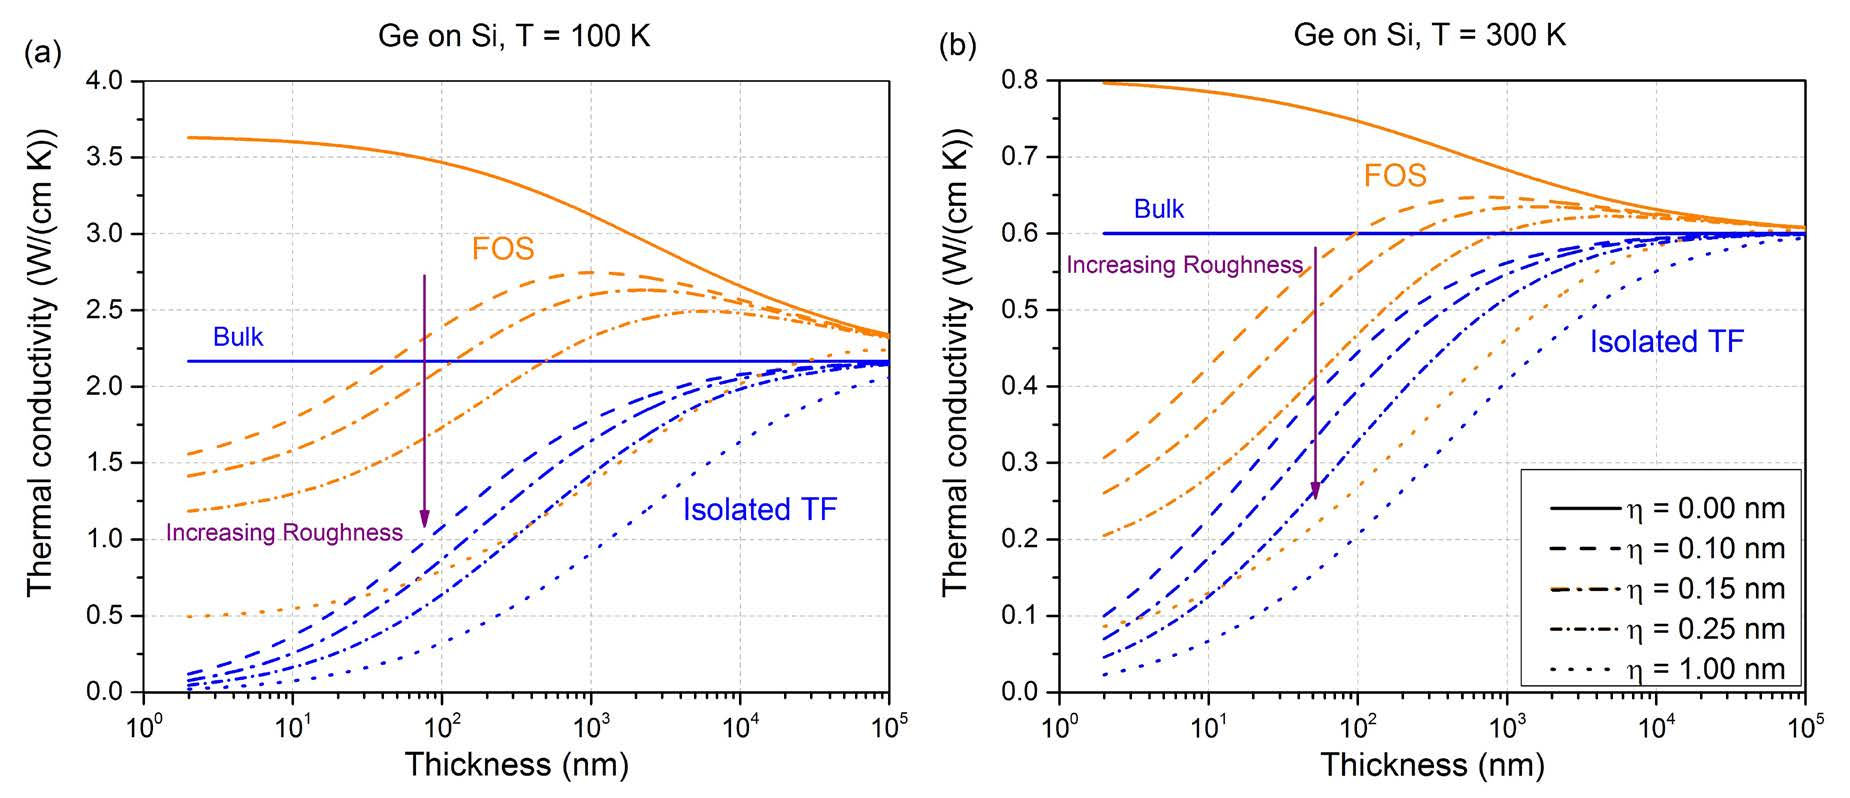
\includegraphics[width=1.0\textwidth]{figures/ch5/Fig5-fos3.jpg}
  \caption{Thermal conductivity of a Ge thin film grown on Si substrate in FOS architecture and an isolated free-standing Ge thin film depicted by orange and blue lines respectively for different interfacial roughnesses at temperatures (a) \gls{T} = 100 K and (b) \gls{T} = 300 K. Blue horizontal line corresponds to bulk thermal conductivity of Ge.}
    \label{fig:ch5-fos3}
 \end{figure}
\par In \Cref{fig:ch5-fos3}, we consider an FOS system consisting of a thin film of Ge deposited on a Si substrate, where we study the variation of thermal conductivity of the FOS film and contrast it with that of bulk Ge and an isolated thin film of Ge. Our numerical predictions show that for certain surface conditions and thicknesses the thermal conductivity of the thin film on substrate still increases beyond the bulk Ge thermal conductivity with decreasing thickness but enhancement effects by phonon coupling are less pronounced in this case due to dissimilar dispersion relations for Si and Ge. The thermal conductivity of FOS is also enhanced beyond the corresponding isolated thin film conductivity values. We note that a large acoustic impedance between Si and Ge owing to a difference in densities and phonon mode velocities leads to significant reduction in transmission and phonon coupling in the Si-Ge case. Thus, with decreasing thickness, we generally observe a decrease in the thermal conductivity of the FOS due to increasing diffuse scattering effects. However, for cases where the interfacial diffuse scattering is not the dominant mechanism (for instance, when $\eta$ = 0) the thermal conduction increases since the volume fraction in which the enhancement takes place increases with decreasing spacing. These combined mechanisms for phonon transport (phonon coupling and interface scattering) also explain the maxima observed in the thermal conductivity of the FOS Si-Ge system. We also mark that the thermal conductivity enhancement ($\Delta\kappa_{\text{iso}}$), diminishes with increasing thickness of the thin film. This is due to the reducing influence of surface scattering and phonon coupling and the fact that thin film conductivities tend towards the bulk conductivity with increasing thickness. We also show in \Cref{fig:ch5-fos3} the impact of surface conditions and temperature variation and find how the thermal conductivity and its enhancement increases with reduction in surfaces roughness and temperature.
\par In contrast to established thermal transport in thin-films, we showed that it is possible to increase the in-plane thermal conductivity of a thin film by placing it on top of an appropriate substrate and that the thermal conductivity increases with decreasing spacing. We observe enhancement of thermal conductivity in FOS architecture beyond the predictions for bulk and isolated thin-film and study its behavior with changing thickness, roughness and temperature. AlGaAs on GaAs and Ge on Si, as considered in this chapter, are widely used as fundamental units in electronic and optoelectronic applications. The analysis of these FOS architectures suggests that experimental measurement of thermal conductivity of thin-films needs to account for thermal coupling between thin film and substrate and the consequent conductivity modification and indicates the need to develop rigorous conductivity read-out model for experiments. 
\section{Summary}
In this chapter, we presented a novel approach of phonon spectral coupling to modulate the thermal conductivities of nanomaterials. We first analyzed the underlying reasons behind thermal conductivity reduction of cladding Si layers in a Si-Ge-Si architecture with simultaneous thermal conductivity enhancement of embedded Ge layer. We also investigated the thermal conductivity of each layer in a Si-Ge bi-layer architecture which was extended to the experimentally important case of film-on-substrate systems. The overall phenomena underlying these modifications were discovered to be phonon injection due to spectral coupling across the interfaces in these materials. The complex nature of this injection mechanism manifests itself in unique and novel modifications to thermal conductivities. The enhancement and reduction in thermal conductivities depends on both structural and materials properties. The findings in this study are a critical step toward achieving a comprehensive control over the thermal properties of materials. By providing capabilities to enhance thermal conductivities, technologies such as microelectronics can be made more efficient by achieving high thermal dissipation rates. At the same time, reducing thermal conduction by combining phonon spectral coupling and current diffuse scattering approaches can improve the performance of thermoelectrics. The proposed phonon spectral coupling to modulate heat conduction advances the current understanding of phonon transport in nanostructures, creating new opportunities for thermal materials design and development.



%%%%%%%%%%%%%%%%
% Chapter 6
%%%%%%%%%%%%%%%%

%!TEX root = thesis.tex
\chapter{Cross-Plane Thermal Transport in Superlattices}
\label{chap:slxp}
\section{Introduction}\blfootnote{Portions of this chapter have originally been published in \cite{ownSLXP} "Cross-plane Thermal Conduction in Superlattices: Impact of Multiple Length Scales on Phonon Transport" (2019), \textit{Journal of Applied Physics}, Vol. 125 (044304). Reproduced with permission from AIP Publishing.} 
A superlattice is a periodic structure of layers of two (or more) materials. Typically, the thickness of one layer is in the order of nanometers \cite{RN999}. Semiconductor superlattices are central to optoelectronic devices \cite{RN1000,Faist553,book_rogalski_infrared} including photodetectors, quantum cascade lasers and modulators. From the point of view of  thermal transport phenomena in nanoscale semiconductor superlattices, the changes in their properties arise from altered phonon transport dynamics, which can be broadly categorized into coherent and incoherent phonon effects. The term coherent refers to the underlying requirement of phase-preservation between phonons incident on and reflected from an interface between two materials. This condition for coherency, if satisfied across multiple interfaces, can manifest itself in a number of novel modifications of phonon dispersion relations including zone-folding effects, edge-flattening, and opening of thermal bandgaps under certain conditions of periodicity, wavelength, and phonon mean-free-paths \cite{RN362,RN132,RN253,RN394,RN329,RN399,RN393}. On the other hand, incoherent phonon effects result in a modified thermal transport dynamics due to reduced mean-free-paths or deviation in populations from Bose-Einstein distribution of phonons because of phonon-boundary scattering events (see \Cref{chap:predictive,chap:nt}, for example). Although both phonon dynamics (coherent and incoherent) arise from fundamentally different phenomena (i.e., phase preservation and diffuse scattering, respectively), they are controlled by the interaction of phonons with interfaces. This strong underlying connection of nanostructure surfaces to thermal transport coupled with (a) the existence of multiple interfaces and (b) a periodical pattern of these interfaces makes semiconductor superlattices a perfect choice for understanding heat conduction. 

The phenomenon of thermal phonon conduction in any periodic structure, including superlattices, is dependent on multiple key length scales [\Cref{fig:sl_schematic}] which are (i) the total size of the structure \gls{slsize}, (ii) the periodicity of the  structure \gls{period}, and (iii) interface surface properties, i.e., roughness \gls{eta} and correlation length \gls{cl}. In addition, the phonon length variables (iv) mean-free-path \gls{mfp} and (v) wavelength \gls{wl} are integral to the conduction phenomenon. A complex interplay between effects occurring at these various length scales coupled with the broadband nature of phonons determines the overall transport of heat in nanostructures. 
%Fig Schematic
\begin{figure}%[hbt!]	
	{\centering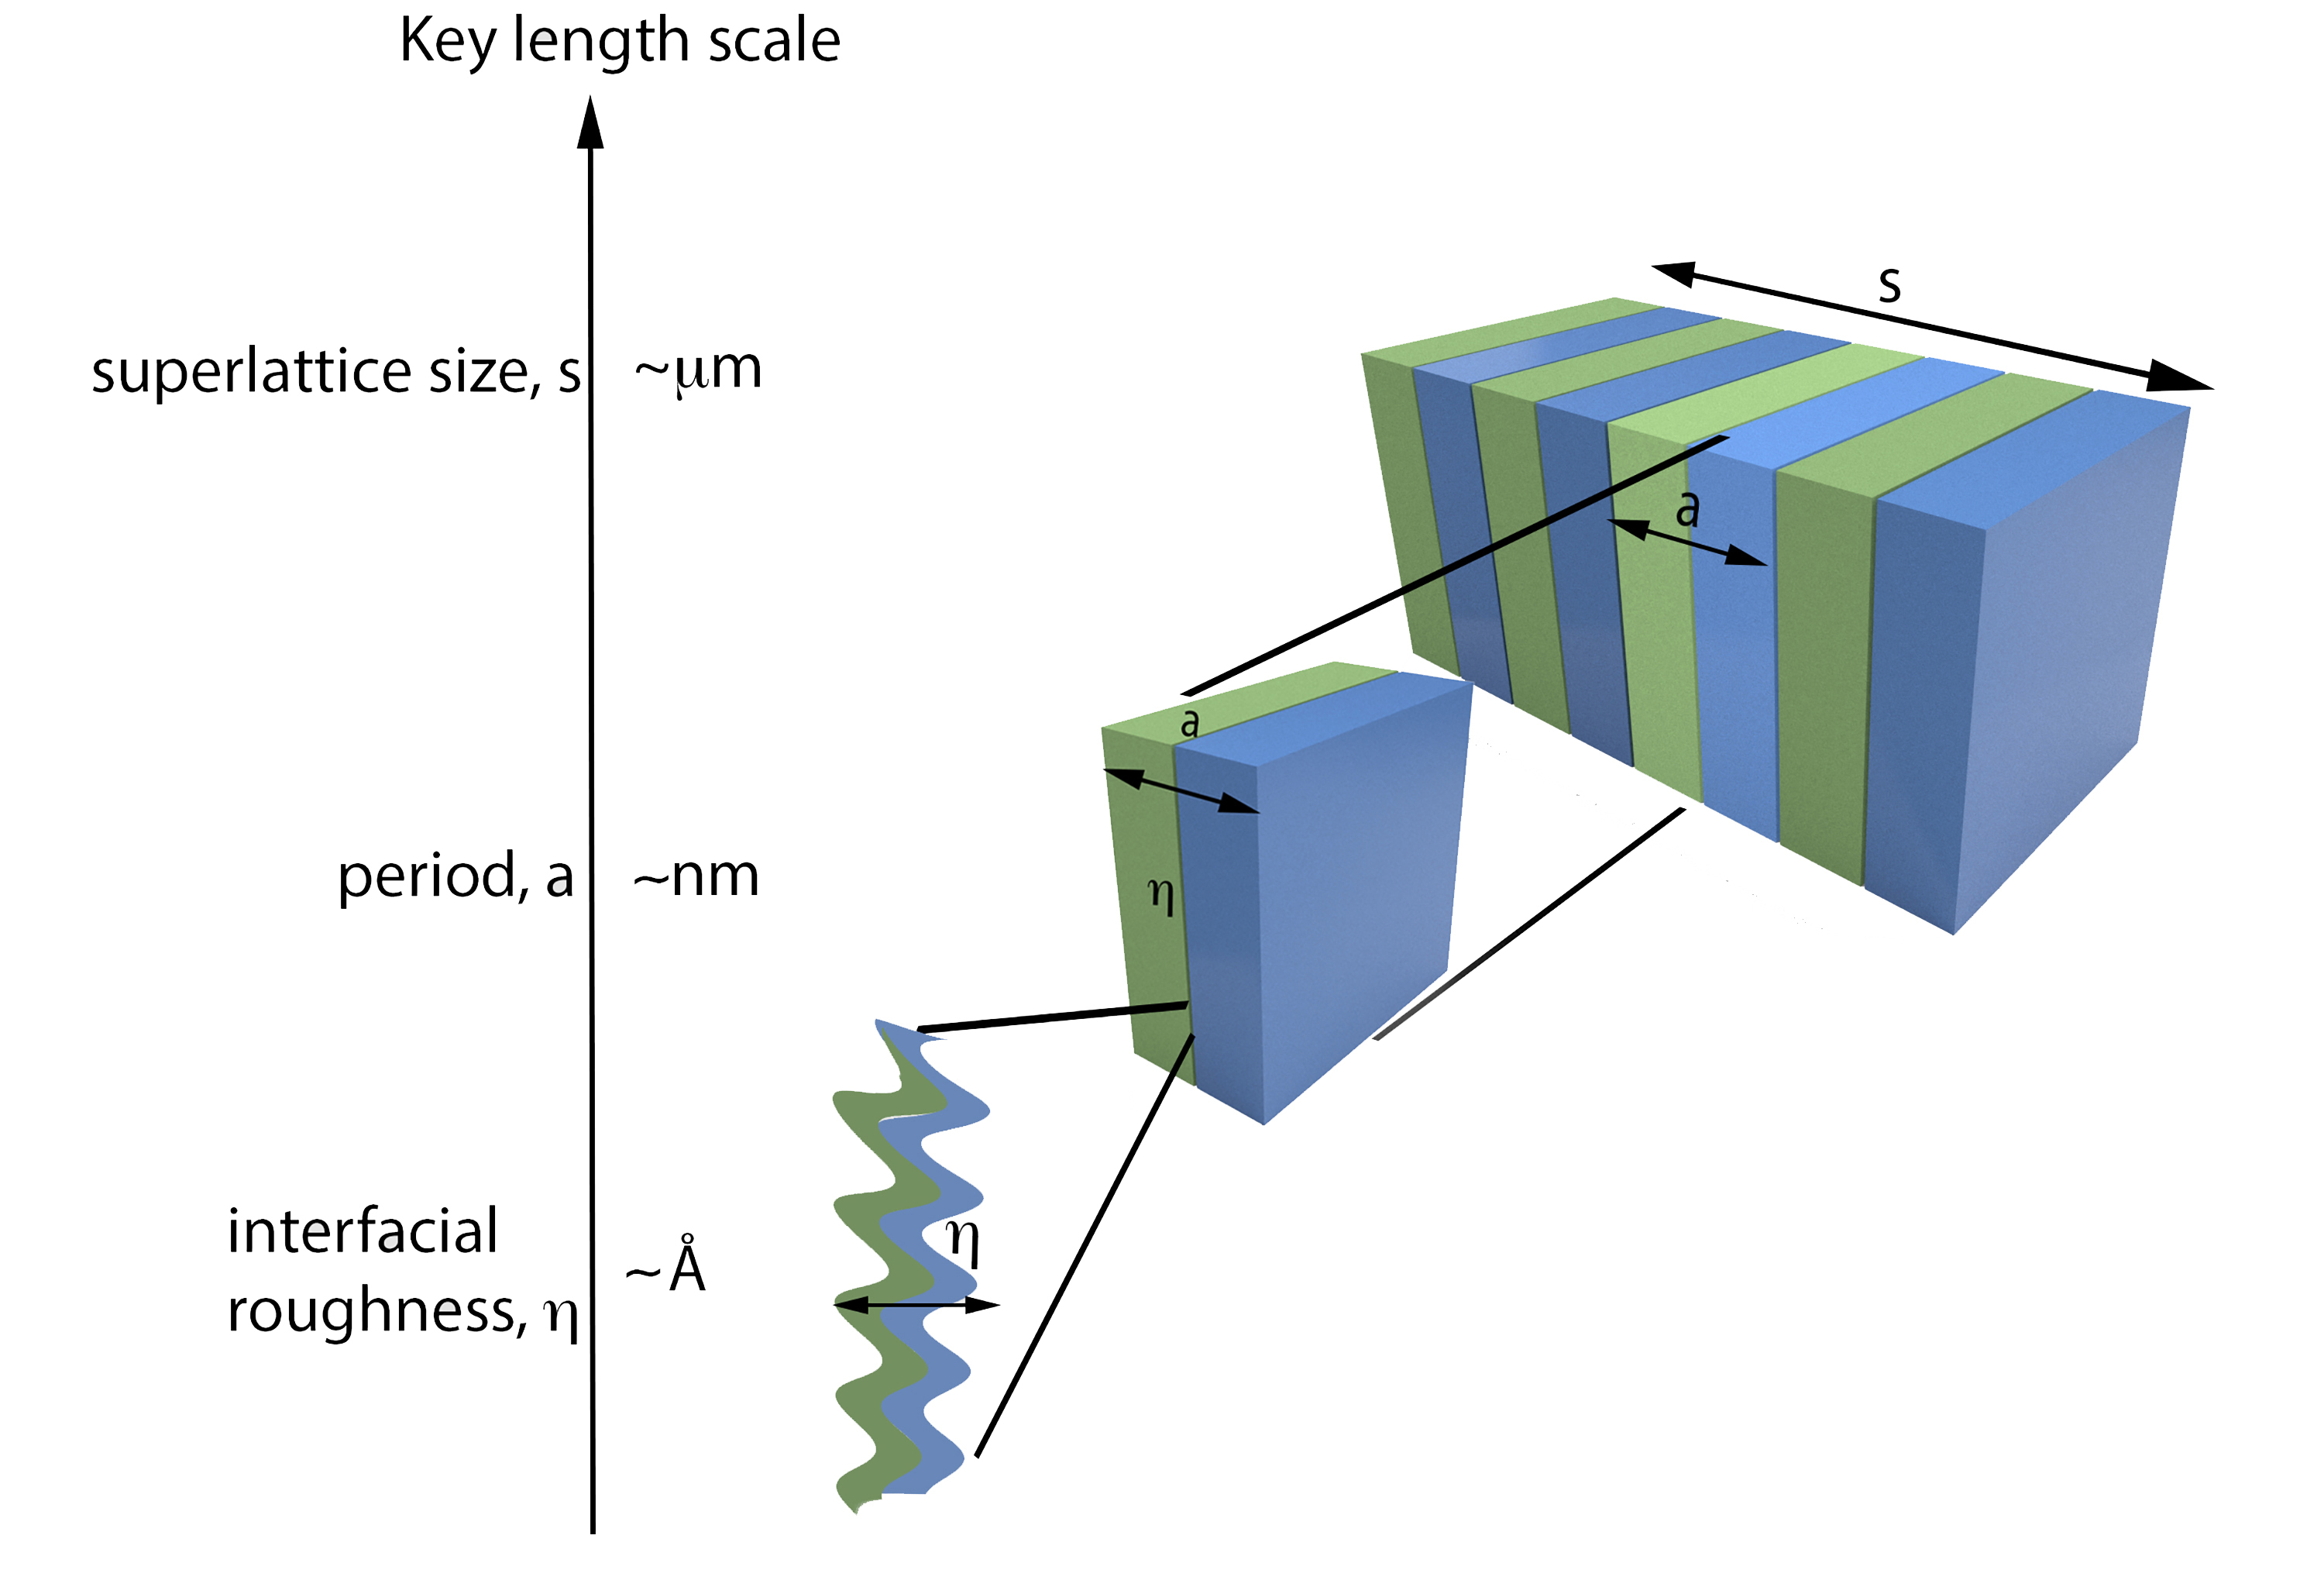
\includegraphics[width=0.93\textwidth]{/ch6/schematic.jpg}}
	\caption{Schematic showing key multiple length scales that control thermal conduction in superlattice structures. Thermal phonons scatter at rough interfaces ($\sim$\angstrom) between each layer within a unit cell of period \gls{period} ($\sim$nm) which combine to create a periodic superlattice nanostructure of total size \gls{slsize} ($\sim$\si{\micro}m).}
	\label{fig:sl_schematic}
\end{figure}

Despite several works over the last few decades, a clear understanding of the role of these fundamental length scales in phonon transport in superlattices remains lacking. For instance, a transition from coherent to incoherent thermal transport effects is expected in smooth-surface superlattices with increasing period length \gls{period}. The transition manifested as minima in thermal conductivity as a function of period has been shown in a few specific materials to date \cite{RN393,RN551}, indicating a need for an in-depth understanding of thermal transport in these structures. In addition to multiple reflections, the layered arrangement in a superlattice also creates an anisotropy in the structure that differentiates between heat flow parallel (in-plane) or perpendicular (cross-plane) to the interfaces, making them useful as directional heat spreaders for electronics \cite{RN545}. %

\section{Literature Overview of Si/Ge Superlattices}
Silicon and germanium are two popular and important semiconductors of commercial importance, and superlattices composed of these elements had attracted significant attention in experimental works. The work by Lee \etal \cite{RN282}, Borca-Tasciuc \etal \cite{RN298}, and Huxtable \etal \cite{RN361,RN297}, remains the primary source of experimental data for the cross-plane thermal conductivities in Si/Ge superlattices. All of these works alluded to the importance of the interface quality and defect density -- features which are still poorly quantified and understood-- in their thermal conductivity measurements. As noted in a recent study \cite{RN544}, the absence of consistency among the measured thermal conductivities in many of these studies \cite{RN282,RN298,RN300}, leaves a gaping hole in our understanding of thermal transport in these superlattices. From a theoretical standpoint, numerous techniques have been developed to understand thermal transport in superlattices \cite{RN266,RN264,RN305,RN306,RN357,RN353} but quantitative predictions of thermal transport properties in realistic nanostructures, accounting for interfacial scattering and phonon-phonon scattering across all temperatures, continue to be an open challenge. A quick glimpse at the literature reveals the underlying dissonance in the predictions by theoretical models. For instance, first-principle calculations and the Boltzmann transport equation (BTE) showed that interfacial roughness serves to reduce the thermal conductivity in Si/Ge superlattices \cite{RN328,RN294,RN169}. In contrast, Green function calculations predicted that lattice thermal conductivity of Si/Ge superlattices with rough interfaces could be higher than those with smooth interfaces if the number of periods were small \cite{RN295}. Furthermore, molecular dynamics \cite{RN319,RN353,RN262} have noted that the absence of a coherent transport signature (i.e., thermal conductivity minimum with period length) could be explained by the interfacial roughness in Si/Ge superlattices. First-principle approaches, on the other hand, showed that even after inclusion of interfacial disorder as perturbations, minima in thermal conductivity could still be observed \cite{RN262}. Thus, there is a clear need for a detailed study of cross-plane thermal transport in Si/Ge superlattices, addressing the role of interfaces and impact of all other relevant length variables on thermal conductivity, i.e., the periodicity \gls{period}, the mean-free-path of phonons \gls{mfp}, wavelength of phonons \gls{wl}, and total size/thickness of the structure \gls{slsize}.
\par Theoretical approaches based on the phonon Boltzmann transport equation (BTE) hold an untapped potential in being able to effectively connect theoretical predictions with experiments. The flexibility of BTE approaches allows for treatment of heat transport in various geometrical domains without relying on limiting assumptions about surface properties. Historically, BTE based approaches considered the use of fitting specularity parameters that limited the physical insights. However, as we discussed in \Cref{chap:predictive}, it is possible to incorporate rigorous surface description within the Boltzmann framework, which can be used to provide quantitative predictions on thermal transport. Moreover, using first-principle calculations to yield material-specific phonon properties as inputs to BTE can create accurate, computationally cost efficient, and comprehensive predictive models for experimental nanostructures provided that the treatment of phonon-interface behavior can be rigorously included. Specifically, for superlattices, the radiative/intensity form of BTE for superlattices \cite{RN267,RN348} dealing with an overall scalar intensity of phonons rather than with individual mode dependent populations precludes the inclusion of incident angle dependent interface-phonon scattering. Recently, solutions to BTE based on the treatment of boundary scattering without transmission between different layers have been developed \cite{RN328,RN372}. Rigorous solutions to the BTE with detailed boundary conditions to obtain local mode dependent phonon populations have been applied to heat transport problems in thin-films, nanowires, (see \Cref{chap:predictive,chap:diff_boundary}) and recently to in-plane thermal transport in layered nanomaterials \cite{RN396} (also see \Cref{chap:layered}). However, such a rigorous approach dealing with mode-by-mode calculation of phonon populations while accounting for interfacial surface characteristics, incident phonon properties, and phonon coupling is currently absent for cross-plane thermal transport in superlattices.
\section{Methodology}
The methodology is based on the layered nanomaterials solution discussed in \Cref{chap:layered}. The general first-order solution to the phonon Boltzmann transport equation under a small temperature gradient in the \textit{cross-plane} $x$ direction, can be written as \cite{ownSLXP},
\begin{equation} 
  g_i^\pm=  -v_{i|x} \tau_{i}\frac{\partial T}{\partial x}\frac{\partial f_{i}^{BE}}{\partial T}\Bigg(1+\Phi_{i}^\pm\exp\Big(-\dfrac{x}{\tau_{i} v_{i|x}}\Big) \Bigg)
\label{eq:ch6-gpm}
\end{equation}
Despite the similarity to \Cref{eq:ch5-gpm}, here the dependence of deviation function $g^\pm$ is independent of the z-dimension. We note that the deviation function depends on the direction of phonon propagation indicated by + and - symbols for propagation along the applied thermal gradient and opposite to the applied thermal gradient, respectively. Since the superlattice is comprised of periodically repeating unit cell, an interfacial phonon balance at the unit cell interface \cite{RN396} along with an anti-symmetric deviation from equilibrium for phonons moving in opposite directions in the superlattice \cite{RN582} are sufficient conditions to solve for deviation functions in the cross-plane direction. Individual layers thermal conductivities are obtained using \Cref{eq:pop_fourier}. The overall cross-plane thermal conductivity of the superlattice structure is evaluated by considering flux conservation in the direction of the thermal gradient. Due to the presence of interfaces between the two materials in adjoining layers of the superlattice, the temperature gradient across the interfaces would change abruptly, which is accounted for using the thermal boundary resistance ($R_\textrm{TBR}$) \cite{RN328}. Thus, the cross-plane thermal conductivity $\kappa_\textrm{cp}$ of the superlattice can be expressed as,
\begin{equation} 
\dfrac{t_1+t_2}{\kappa_\textrm{cp}}=\dfrac{t_1}{\kappa_1}+\dfrac{t_2}{\kappa_2}+R_\textrm{TBR}
\end{equation}
where $t_1$ and $t_2$ are, respectively, the thicknesses of the two constitutive layers of the superlattice and $\kappa_1$ and $\kappa_2$ are the individual thermal conductivities of the layers.
\section{Key Results and Discussion}
%Figure2
We first predict the thermal conductivity of Si/Ge superlattices at room temperature (\gls{T} = 300 K) in \Cref{fig:ch6-2}(a) and low temperature (\gls{T} = 80 K) in \Cref{fig:ch6-2}(b). We show how the thermal conductivity increases with increasing period thicknesses for different superlattice interface conditions ranging from very smooth to very rough surfaces. The increasing period thickness a reduces the interface density and allows phonons to travel longer distances between scatterings from interfaces. The reduction in interface density thus directly translates to increased phonon mean-free-paths and thermal conductivities. Interestingly, we observe that even at large period thicknesses (\gls{period} $\sim$ 5 \si{\micro}m), the thermal conductivity is below the value in the absence of phonon-surface scattering (i.e., bulk value), indicating the wide spectrum of phonon mean-free-paths and the strong interface scattering phenomenon in cross-plane phonon transport. The thermal conductivity predictions for different roughness values converge at larger period thicknesses owing to the reduced interface scattering events, removing the difference arising due to diffuse scattering. Interestingly, for small period \gls{period} $\sim$ 5 nm at low temperature \gls{T} = 80 K, introduction of a slight degree of disorder (\gls{eta} $\sim$ 0.05 nm) leads to a strong reduction in superlattice thermal conductivity. In this case, the small periodicity of the superlattice coupled with the reduced phonon-phonon scattering at low temperatures allows phonons to scatter strongly from the introduced disorder at the surfaces. Furthermore, it is observed that the increase of surface roughness from \gls{eta} = 0.5 nm to \gls{eta} = 1.0 nm leads to a minimal change in cross-plane thermal conductivity, indicating the onset of nearly complete diffusive scatterings at these roughnesses in these structures. We also plot in \Cref{fig:ch6-2} the experimentally measured thermal conductivities in Si/Ge superlattices and find excellent agreement despite the variability in the experimental data. We note that experimental growth of superlattices relies on the use of buffer layers as well as the use of surfactants whose presence in samples could influence the measured thermal conductivity \cite{RN361,RN297,RN298,RN300}. These experimental factors (e.g., the role of buffer layers, creation of native oxides, etc.) are not included in our model which is aimed at understanding the role of all length scales in thermal transport.
\begin{figure}[hbt]
  \centering 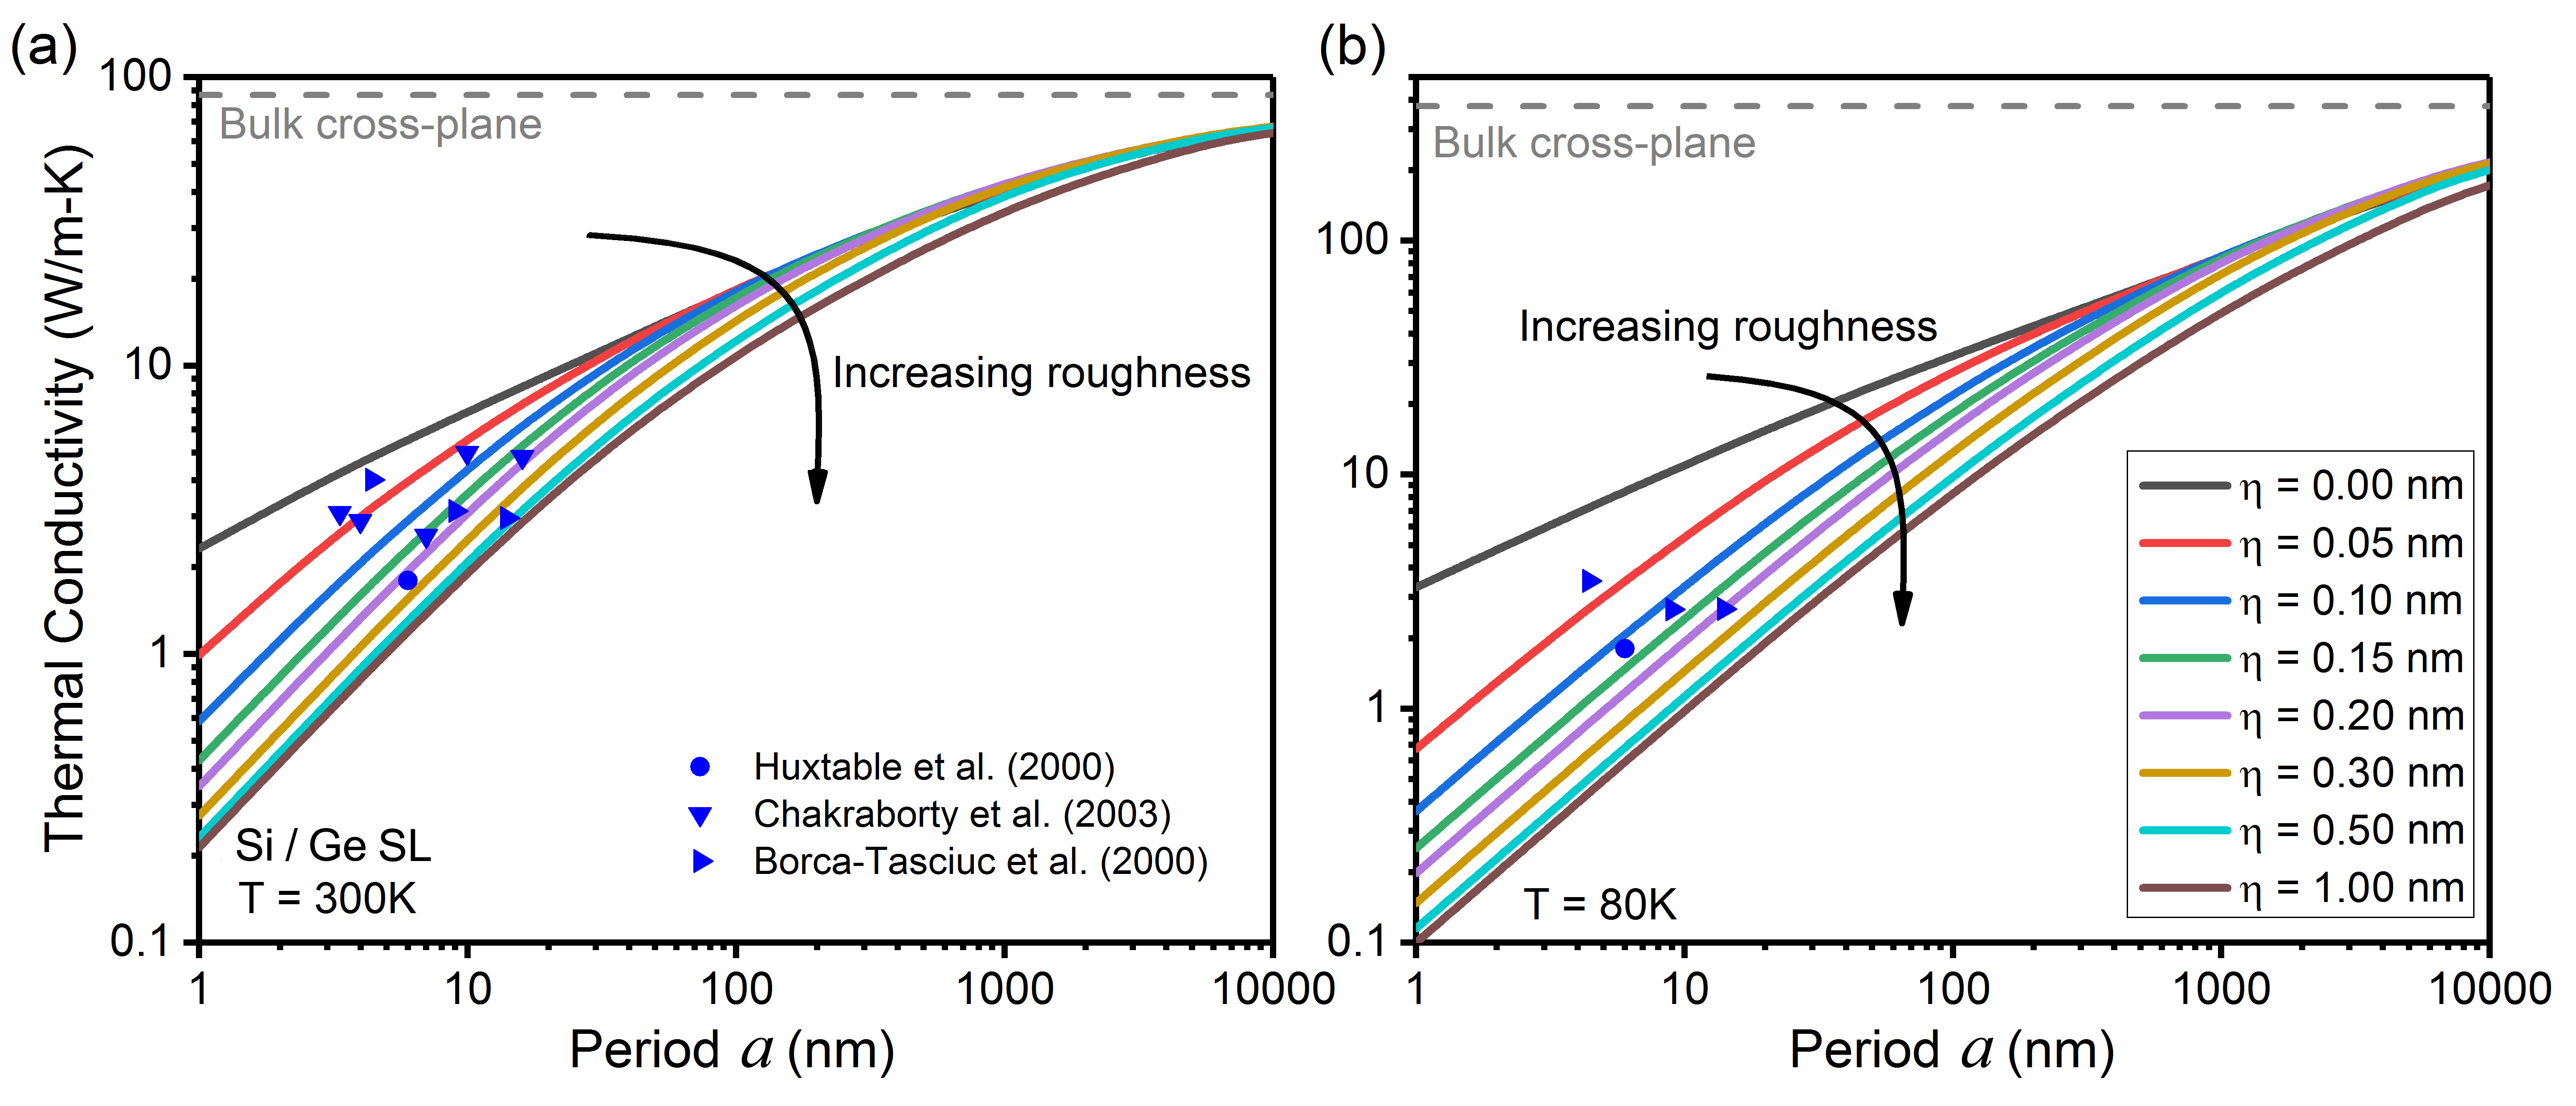
\includegraphics[width=1.0\textwidth]{figures/ch6/Fig2.jpg}
  \caption{Cross-plane thermal conductivity \gls{K} in Si/Ge superlattices at (a) \gls{T} = 300 K and (b) 80 K as a function of period thickness \gls{period}. \gls{K} predictions for different interfacial roughnesses \gls{eta} are shown and compared against available experimental data (scatter points).}
  \label{fig:ch6-2}
\end{figure}
%Figure3
Additionally, the large contrast in lattice constants between Si and Ge unit cells heightens the challenge of obtaining a control over interfacial roughness experimentally, which is a key factor in determining thermal transport in nanostructures \cite{RN396}. Note that our analysis is focused on phonon transport in the absence of coherent interference effects. It is expected that a high interfacial roughness in experimental Si/Ge superlattices prevents coherent effects from playing a dominant role \cite{RN544}. Our findings clearly show the importance of interface conditions, in particular for small period superlattices, as they can yield strong modulations in thermal transport, reinforcing the need for quantitative approaches to model and report superlattice surface conditions. In \Cref{fig:ch6-3}(a) and (b), we also compare our numerical predictions against experimental measurements on \sige{0.84}{0.16}/\sige{0.76}{0.24} alloy superlattices with equal volume fractions \cite{RN361}. We find excellent agreement with the experimental measurements and observe that the thermal conductivity has a very weak dependence on interfacial roughness in these superlattices. The weak dependence on interfacial scattering can be explained by the material similarity of the superlattice layers, which reduces the influence of roughness on phonon transmission at interfaces. For a different experimental data-set of Si/\sige{0.70}{0.30} superlattices with two-third of volume fraction comprised by the Si layer \cite{RN361}, we observe qualitative agreement with the data at \gls{T} = 300 K but we find that the reported thermal conductivities are larger than the numerical predictions. The dependence of thermal conductivity on surface roughness is observed to be stronger unlike the \sige{0.84}{0.16}/\sige{0.76}{0.24} case, since the materials across interfaces are more distinct. Thus, future experimental work with quantification of surface roughness especially in alloy superlattices would be an exciting avenue to experimentally validate the predictions of our model as well as advance the understanding of thermal transport in these nanostructures. Since surface roughness and correlation length are statistical quantities, techniques that can extract and combine surface profiles across the length of the interface are needed. Such techniques involving stitching of transmission electron microscope (TEM) images to extract surface profiles followed by background elimination \cite{RN131} have been used for nanowires while similar efforts for superlattices are currently lacking. 
\begin{figure}[hbtp]
  \centering \includegraphics[width=1.0\textwidth]{figures/ch6/Fig3.jpg}
  \caption{Cross-plane thermal conductivity in experimental alloyed superlattices as a function of period, for different interfacial roughness values. Thermal conductivities are evaluated at \gls{T} = 300 K in [(a) and (c)] and 80 K in [(b) and (d)]. Panels (a) and (b) are for \sige{0.84}{0.16}/\sige{0.76}{0.24} superlattices and (c) and (d) are for Si/\sige{0.70}{0.30} superlattices.}
  \label{fig:ch6-3}
\end{figure}
%Figure4
\par Based on the large number of SiGe alloy superlattice experiments, an interesting question that has not been answered is the impact of alloying one layer vs both layers in the superlattice. To address this question, we consider three possible configurations of alloying, i.e., we alloy either one of the two layers of a Si/Ge superlattice, and also alloy both the layers, and compare all configurations against an unalloyed Si/Ge superlattice. We show in \Cref{fig:ch6-4} the corresponding numerical predictions for the thermal conductivities for different periods, temperatures, and interface conditions. We find that the thermal conductivity in all the superlattices increases with increasing period \gls{period}, irrespective of the inner surface condition, temperature, or alloying. These results are in agreement with an earlier report \cite{RN267} and can be understood by the increased effective mean-free-paths with increasing distance between the boundaries under incoherent transport. However, unlike the conclusions of this report, we find that the thermal boundary resistance does not play a determining role in our predictions. We note that it has also been reported \cite{RN291} that thermal transport in superlattices cannot be attributed solely to thermal boundary resistance. In our calculations, one order change in thermal boundary resistance (TBR) at room temperature from $3\times 10^{-9}$ \si{\meter\squared\per\kilo\watt}  \cite{RN358} (value used in this report) to $3\times 10^{-8}$ \si{\meter\squared\per\kilo\watt} leads to a negligible change in the thermal conductivity (\textless1\% at \gls{period} = 5 nm), quantifying the small impact TBR has on thermal conductivity value of the Si/Ge superlattices. This finding can be understood by an order of magnitude analysis on individual resistances of the Si and Ge layers, and the effects of TBR between the layers, which becomes small with increasing period. Interestingly, we observe that the alloying of either of the Si or Ge layers leads to a similar reduction in thermal conductivity (red and blue lines) for all periods and surface conditions. We note that alloying of either of the layers leads to impurity scattering for phonons in the alloyed layer and also for phonons that can couple across the interfaces and travel in both the materials. Since the conductivities of the layers are arranged in parallel, the thermal transport is critically determined by the thermal conductivity of the layer with smaller conductivity. Thus, we conclude that alloying either layer in a Si/Ge superlattice to a small degree leads to similar thermal conductivities. In the case when both the layers are alloyed, phonons in all the layers have reduced mean-free-paths due to scattering by alloy atoms, lowering the thermal transport further (brown lines). This behavior persists for both smooth (\gls{eta} = 0.1 nm) and rough (\gls{eta} = 0.5 nm) inner interfaces. We also observe that the thermal conductivity of unalloyed Si/Ge superlattices especially at low temperatures (e.g., \gls{T} = 80 K) with rough inner interface decreases linearly with decreasing periods for \gls{period} \textless 100 nm [\Cref{fig:ch6-4}(c)], indicative of nearly ballistic transport within the layers at these temperatures.
\begin{figure}[hbt]
  \centering 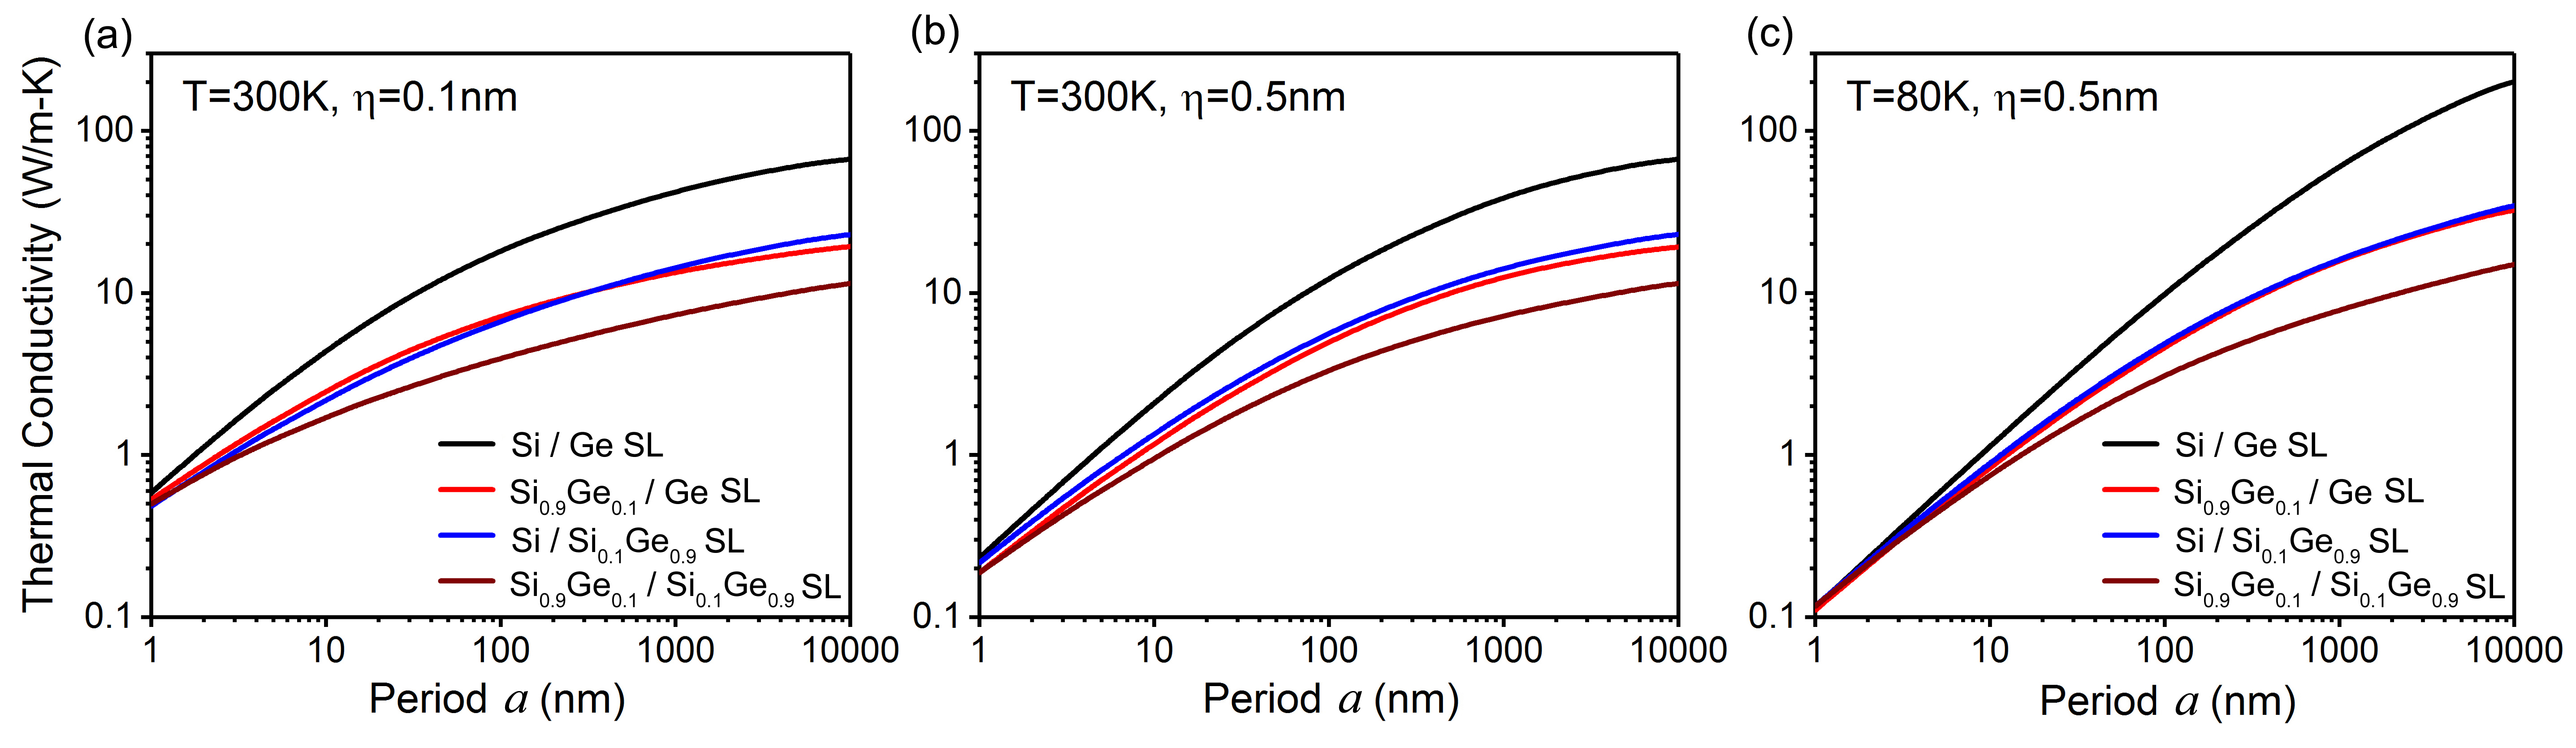
\includegraphics[width=1.0\textwidth]{figures/ch6/Fig4.jpg}
  \caption{Cross-plane thermal conductivity in Si/Ge (black lines), \sige{0.90}{0.10}/Ge (red lines), Si/\sige{0.10}{0.90} (blue lines), and \sige{0.90}{0.10}/\sige{0.10}{0.90} (brown lines) superlattices at (a) \gls{eta} = 0.1 nm and \gls{T} = 300 K, (b) \gls{eta} = 0.5 nm and \gls{T} = 300 K, and (c) \gls{eta} = 0.5 nm and \gls{T} = 80 K, as a function of period thickness \gls{period}.}
  \label{fig:ch6-4}
\end{figure}

%Figure5
\par Importantly, there is also the possibility of quasi-ballistic transport across the entire superlattice structure, which leads to another important length scale -- the total structure size \gls{slsize}. The existence of thermal conductivity that increases linearly with total structure size has been experimentally observed in GaAs superlattices \cite{RN394}, which has been corroborated by a recent study \cite{RN544}. To understand the role of structure size \gls{slsize} on thermal transport in Silicon-Germanium based superlattices, we next use our approach to predict the thermal conductivity in Si/Ge and \sige{0.90}{0.10}/\sige{0.10}{0.90} superlattices as a function of total size for different periods at \gls{T} = 300 K (\Cref{fig:ch6-5}). The finite size of the structure limits the number of periods that can exist in the structure. Strictly speaking, finite sized structures need to be modeled by applying phonon population balance at each surface (i.e. interfaces and boundaries). In our approach, we consider a unit cell of two layers as described in the Methodology and evaluate the thermal conductivity assuming a fully diffusive boundary after a specified number of periods. \Cref{fig:ch6-5} shows that the thermal conductivity of Si/Ge and SiGe alloyed superlattices is significantly influenced by the structure size \gls{slsize} (or number of periods, $N = s/a$), and thus these features need to be reported as well in experiments for consistent comparison between measurements. We observe that for small period superlattices at room temperature [\Cref{fig:ch6-5}(c,d)], a superlattice with smooth interface (solid lines) shows an increasing trend of thermal conductivity with increasing structure size, while for superlattices with rough interfaces (dashed lines), the total structure size change leads to a smaller increase in thermal conductivity. These findings indicate that smoother interfaces allow phonons to cross multiple periods and the total structure size \gls{slsize} becomes a limiting factor in their mean-free-paths. However, for alloyed superlattices [\Cref{fig:ch6-5}(b)], we observe that the structure size \gls{slsize} can influence the thermal conductivities of superlattices with both small and large roughness especially for period \gls{period} = 200 nm due to the existence of large mean-free-path phonons in large period superlattices. To further elucidate the thermal conductivity dependence on structure size in alloyed superlattices without having to consider the variability in individual period size \gls{period}, we added one period at a time in \Cref{fig:ch6-6}. The alloyed superlattice exhibits a significance dependence of \gls{K} on the number of periods, indicative of the large phonon mean-free-paths in these structures. We also find that the effect of adding periods leading to a quasi-linear increase in conductivity persists even at \gls{T} = 300 K highlighting the existence of phonons that can cross multiple interfaces at these temperatures provided the surface roughness is low. The impact of adding periods on conductivity is slightly stronger at \gls{T} = 80 K due to the diminishing phonon-phonon scattering at these temperatures. These results support the conclusion that phonons that can cross multiple interfaces are better observed at low temperatures and smooth interfaces, in agreement with the conclusions for GaAs/AlAs superlattices in Ref. \cite{RN394}. Since multiple interfacial scattering is a key criterion for interference phenomenon, it can be concluded that structures allowing for such large mean-free-path phonons to propagate (i.e., low temperatures and low roughness) would be better candidates to explore coherent interference modifications in thermal transport \cite{RN362,RN394,RN393}.
\begin{figure}[hbtp]
  \centering \includegraphics[width=1.0\textwidth]{figures/ch6/Fig5.jpg}
  \caption{Cross-plane thermal conductivity at \gls{T} = 300 K as a function of total superlattice size \gls{slsize} for [(a) and (b)] large periods \gls{period} = 50 nm and 200 nm, and [(c) and (d)] short periods \gls{period} = 4 nm and 10 nm. The solid lines represent smooth interfacial roughness \gls{eta} = 0.1 nm, and the dashed lines represent surface roughness \gls{eta} = 0.5 nm.}
  \label{fig:ch6-5}
\end{figure}
%Figure6
\begin{figure}[hbt]
  \centering 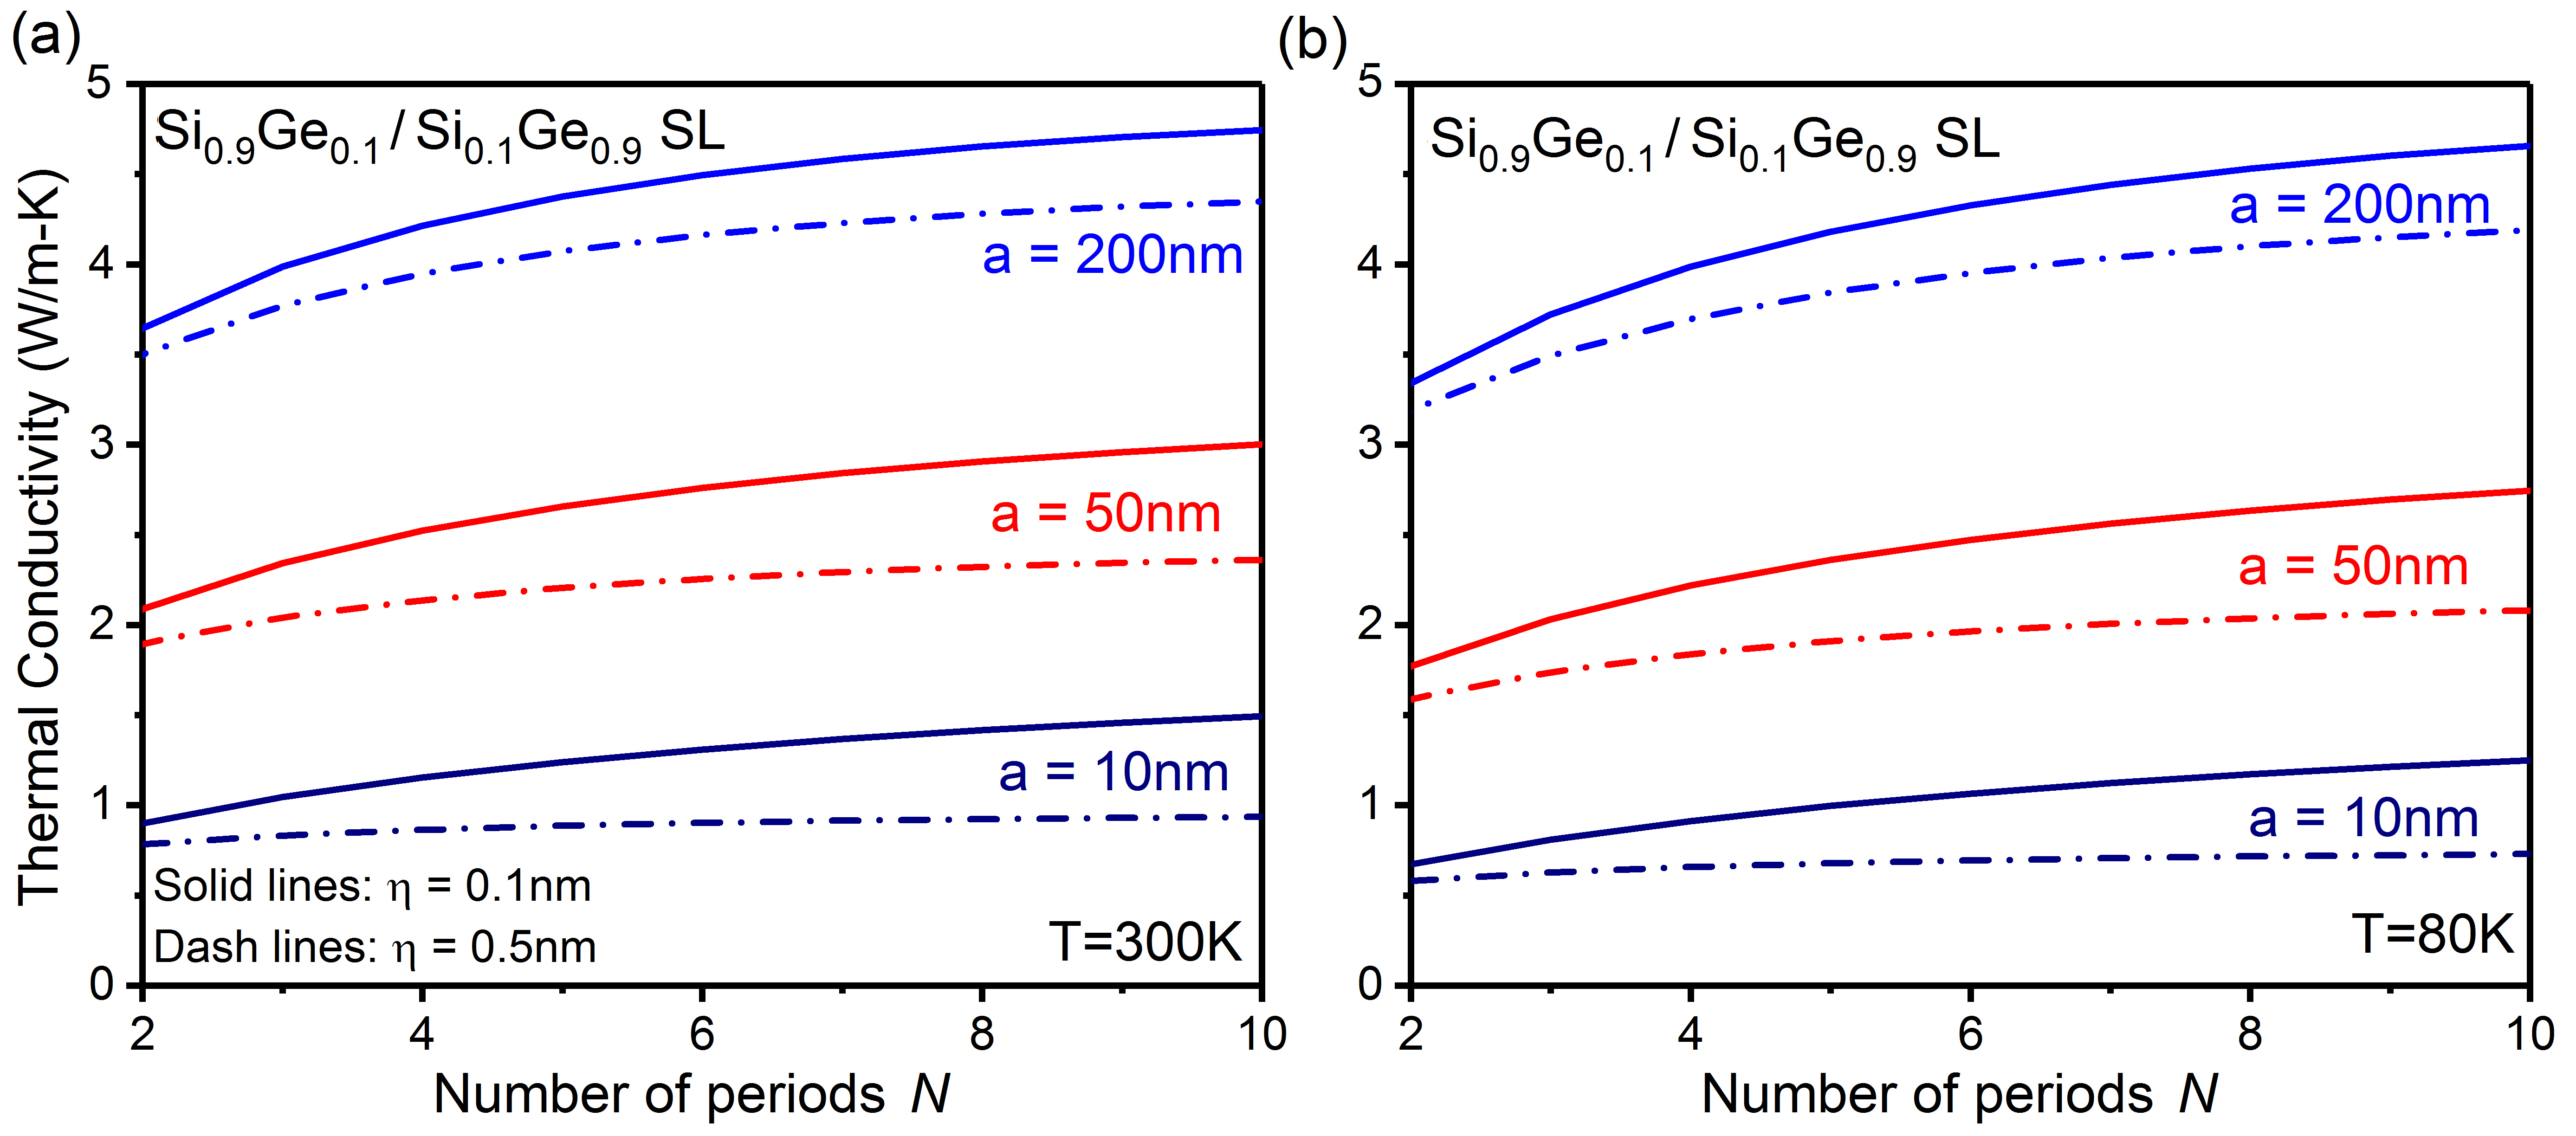
\includegraphics[width=1.0\textwidth]{figures/ch6/Fig6.jpg}
  \caption{Cross-plane thermal conductivity in alloyed superlattices at (a) \gls{T} = 300 K and (b) \gls{T} = 80 K as the function of number of periods $N$ in the superlattice. Three different periods \gls{period} = 10 nm (dark blue), 50 nm (red), and 200 nm (blue) are shown for two different surface conditions.}
  \label{fig:ch6-6}
\end{figure}
%Figure7
\par The layered structure of superlattices creates an anisotropic resistance to heat flow, providing a difference in thermal conductivities in the directions parallel and perpendicular to the interfaces. It is expected that when the thermal gradient is applied parallel to the interfaces (in-plane transport), phonon transport processes face less resistance from the boundaries than when the gradient is applied perpendicular to the interfaces \cite{book_Ziman}. This anisotropy in thermal transport is of great practical interest to create solid-state heat spreaders to better manage heat in electronic devices. We calculate the anisotropy in heat transport at 300 K (red lines) and 80 K (blue lines) in Si/Ge superlattices (\Cref{fig:ch6-7}) for different periods and interfacial conditions. We find that the anisotropy, defined as the ratio of in-plane to cross-plane thermal conductivity, reduces with increasing period \gls{period}. This indicates that with reduced interface density, both in-plane and cross-plane transport converge to the corresponding bulk values. For large roughness values, the diffusive scattering of phonons reduces the anisotropy ratio due to nearly saturated reduction in cross-plane conductivity. In contrast, for a given roughness, the anisotropy at \gls{T} = 80 K is larger than room temperature because at lower temperatures, resistance by phonon-phonon processes is diminished, allowing for the boundary scattering to dominate, which are stronger in the cross-plane direction. Based on the anisotropic thermal conductivities obtained for superlattices, it is clear that the cross-plane direction boundary scattering phenomenon is generally stronger compared to the in-plane direction. To further explore the transport of phonons in the two different directions, we evaluate their thermal spectra, i.e., the contribution of phonons of different wavelengths and mean-free-paths to total thermal transport. The conduction of heat by phonons with different wavelengths (or frequencies) and mean-free-paths is central to nanoscale thermal conduction. Normalized accumulation functions or heat-spectra have been utilized to understand nanoscale thermal transport in other nanostructures \cite{ownNW,RN236}.
\begin{figure}[hbt]
  \centering 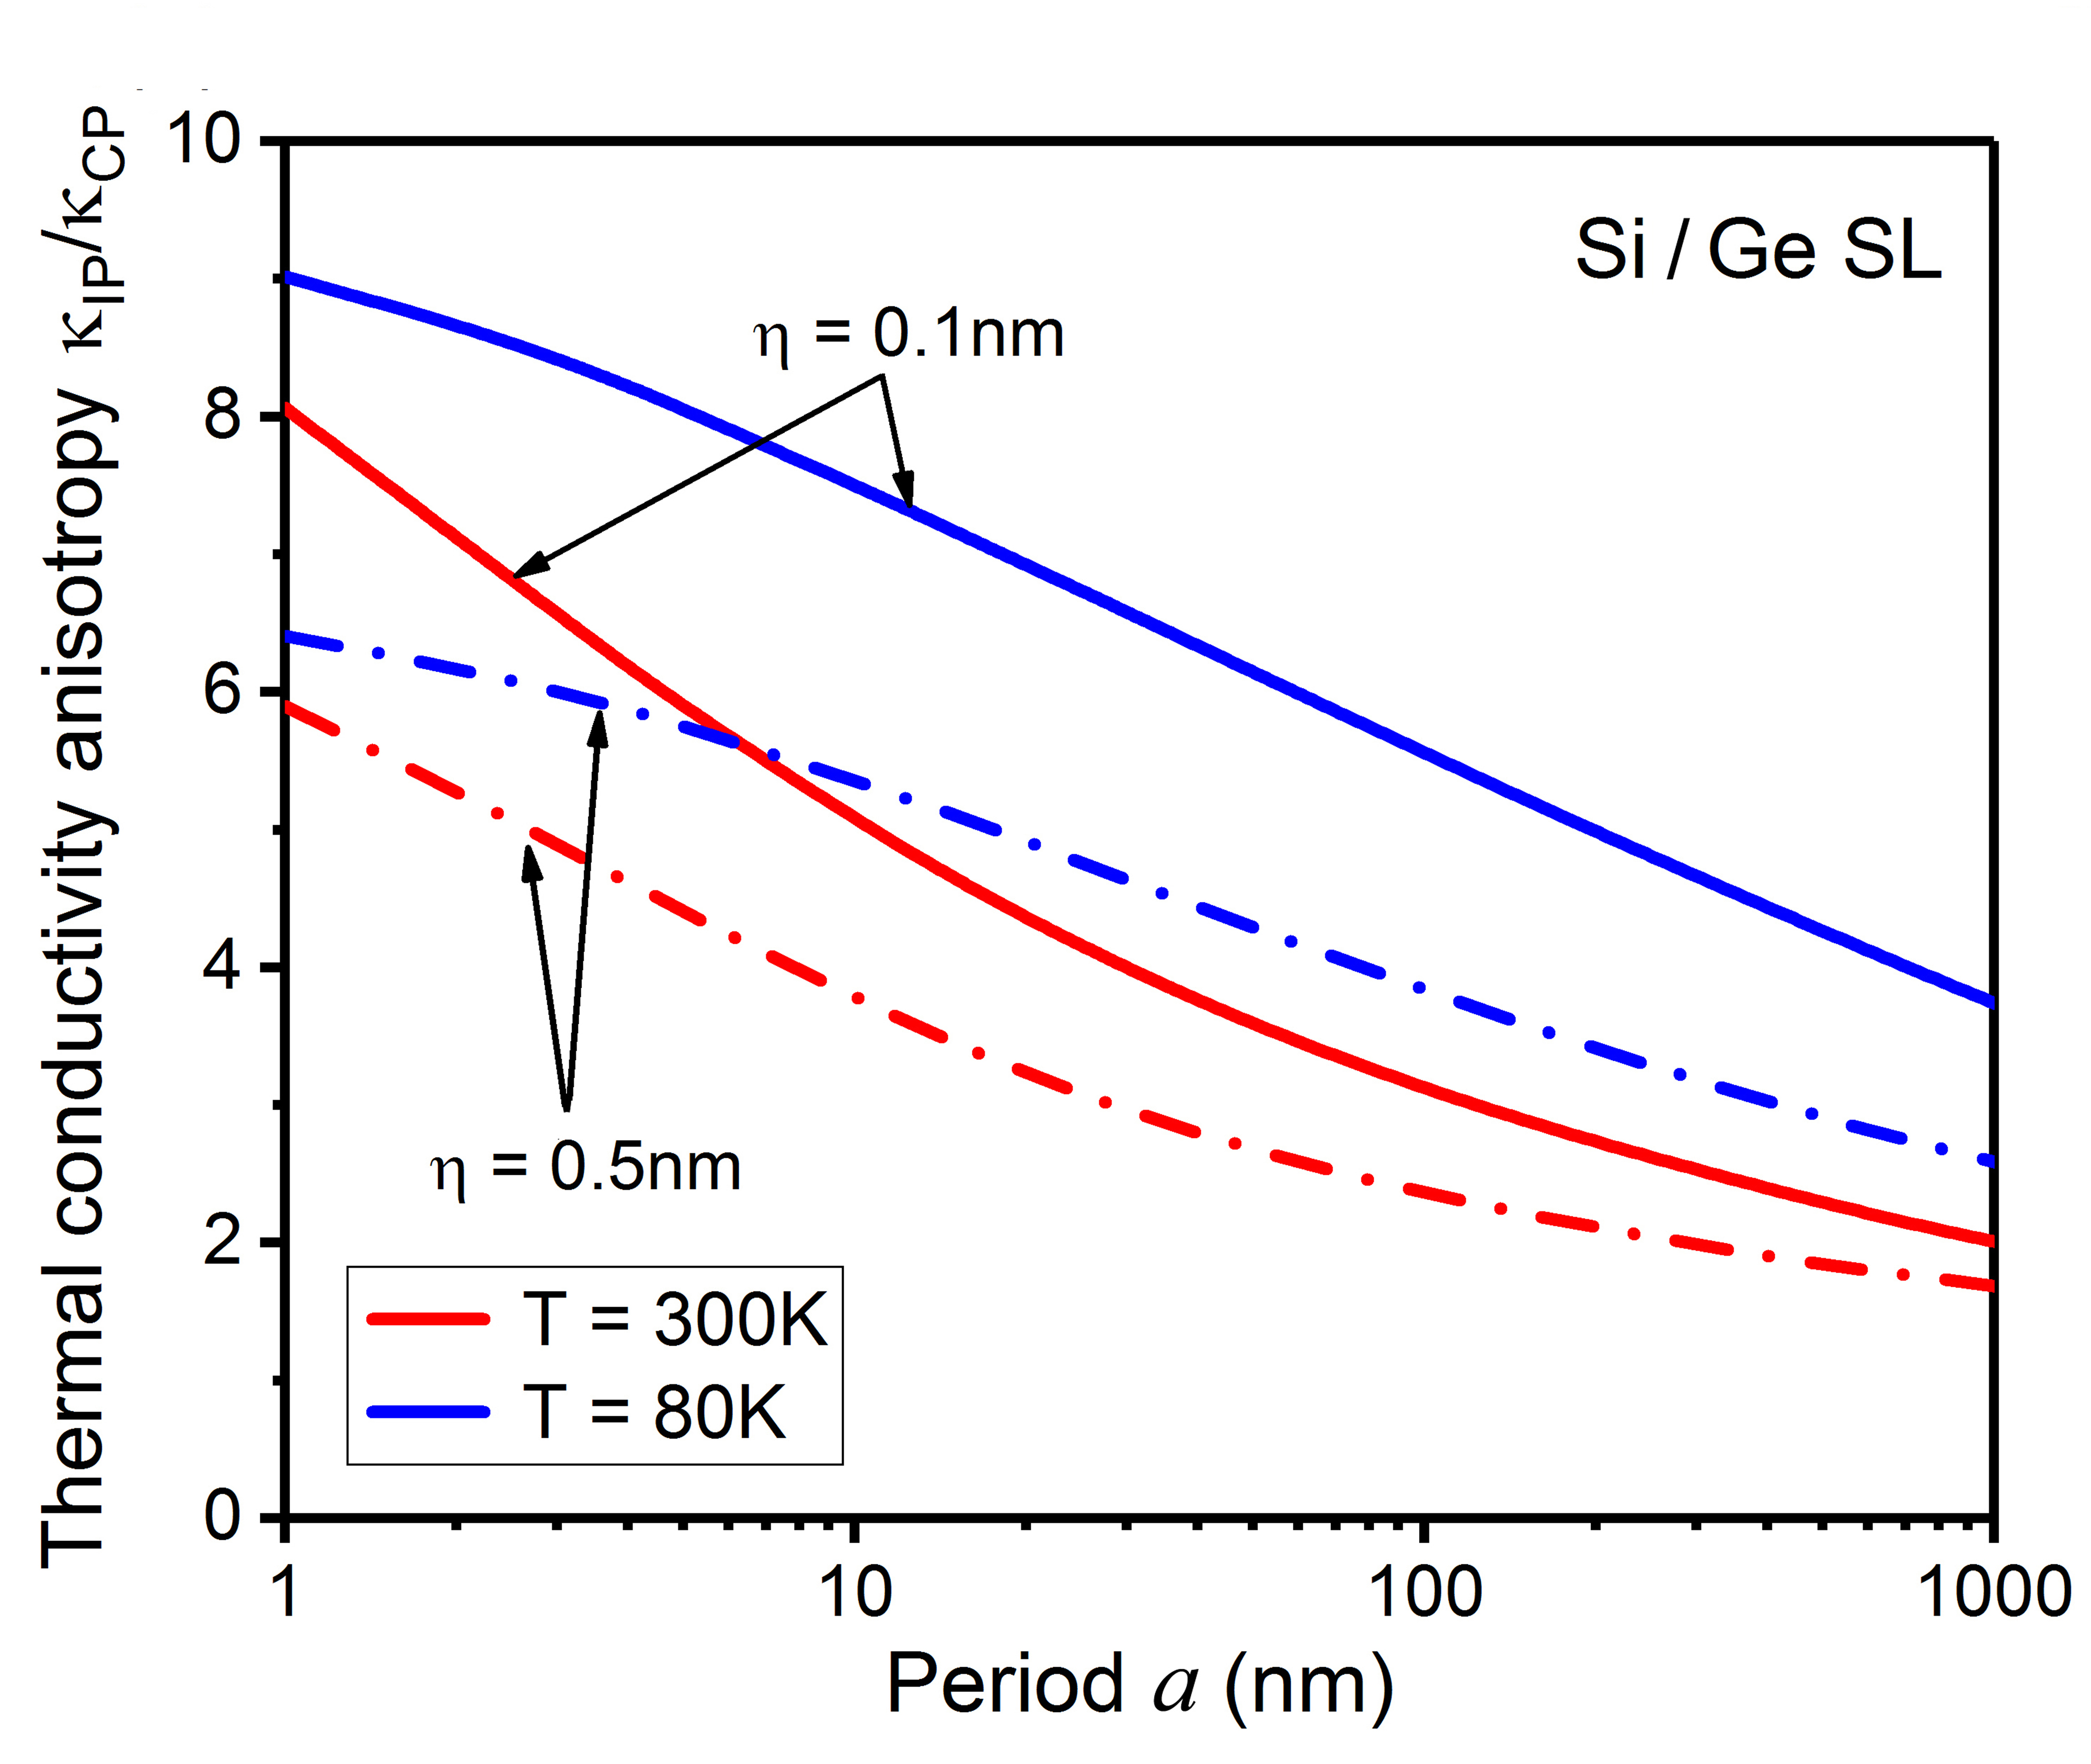
\includegraphics[width=0.80\textwidth]{figures/ch6/Fig7.jpg}
  \caption{The evolution of anisotropy in thermal conductivity with period thickness \gls{period} and roughness \gls{eta} in Si/Ge superlattices at room temperature (red lines) and \gls{T} = 80 K (blue lines).}
  \label{fig:ch6-7}
\end{figure}

%Figure8
\par However, cross-plane thermal transport in superlattices has not received similar attention. Using our developed methodology, we show our predictions for the cross-plane thermal heat spectra as a function of phonon wavelength at room temperature in \Cref{fig:ch6-8}(a,b), and compare it against the in-plane wavelength spectra in \Cref{fig:ch6-8}(c,d) \cite{RN396}. The increased surface scattering of large wavelength phonons caused by rougher interfaces (dashed lines) in all the cases (i.e., in-plane and cross-plane) shifts the thermal spectra to phonons of smaller wavelengths. Furthermore, surface scattering effects are stronger for shorter period superlattices owing to a higher interface density. However, in comparing between cross-plane and in-plane thermal spectra, we observe that the heat conduction in the cross-plane direction is shifted more strongly toward short-wavelength phonons reaffirming the understanding of enhanced surface effects when the gradient is applied perpendicular to interfaces. The difference between cross-plane and in-plane thermal spectra is observed even more clearly for alloyed superlattices. For the cross-plane SiGe alloy superlattice thermal transport [\Cref{fig:ch6-8}(b)], spectra are strongly suppressed such that phonons of wavelength \gls{wl} = 1–10 nm carry nearly all the heat. However, for the in-plane thermal transport, large wavelength phonons (\gls{wl} \textgreater 10 nm) contribute almost 35\% to heat transport for \gls{period} = 50 nm superlattices [\Cref{fig:ch6-8}(d)]. These findings clearly show that in cross-plane superlattice transport, the effects of surface scattering are stronger than in the in-plane direction. In particular, in cross-plane transport, phonons of wavelengths larger than \gls{wl} = 10 nm play no part in thermal transport at room temperature as they are effectively scattered out by scatterings at interfaces.
\begin{figure}[hbtp]
  \centering \includegraphics[width=1.0\textwidth]{figures/ch6/Fig8.jpg}
  \caption{Room temperature wavelength heat spectra for [(a) and (b)] cross-plane and [(c) and (d)] in-plane thermal transport in Si/Ge and \sige{0.90}{0.10}/\sige{0.10}{0.90} superlattices. Two different periods \gls{period} = 10 nm and \gls{period} = 50 nm and roughness values \gls{eta} = 0.1 nm and \gls{eta} = 0.5 nm are considered.}
  \label{fig:ch6-8}
\end{figure}

%Figure9
\par To understand the impact of surfaces on the mean-free-path spectra in superlattices, we consider periods \gls{period} = 50 nm (red lines) and \gls{period} = 10 nm (black lines), as well as surface roughnesses \gls{eta} = 0.1 nm and \gls{eta} = 0.5 nm in \Cref{fig:ch6-9}. We observe that with reducing period length and increasing roughness the heat spectra are shifted to smaller dominant mean-free-paths. This shift can be explained by a stronger interfacial scattering phenomenon in superlattices with smaller periods owing to their higher interfacial density and due to increased diffuse scattering with increasing surface roughness (dashed lines). Our predictions show that in the cross-plane direction heat flow in superlattices of up to period \gls{period} = 50 nm at room temperatures is controlled by phonons in the range of \gls{mfp} = 1–1000 nm. Even in alloyed superlattices where short mean-free-path phonons are scattered out of transport process, the thermal transport is upper bounded by \gls{mfp} = 1000 nm mean-free-path phonons, highlighting the strong role of interfacial scattering in the cross-plane direction. Since the surface properties can strongly influence the thermal transport in the cross-plane direction, quantification of experimental samples and better growth techniques would be the key drivers of future research in these superlattices.
\begin{figure}[hbt]
  \centering 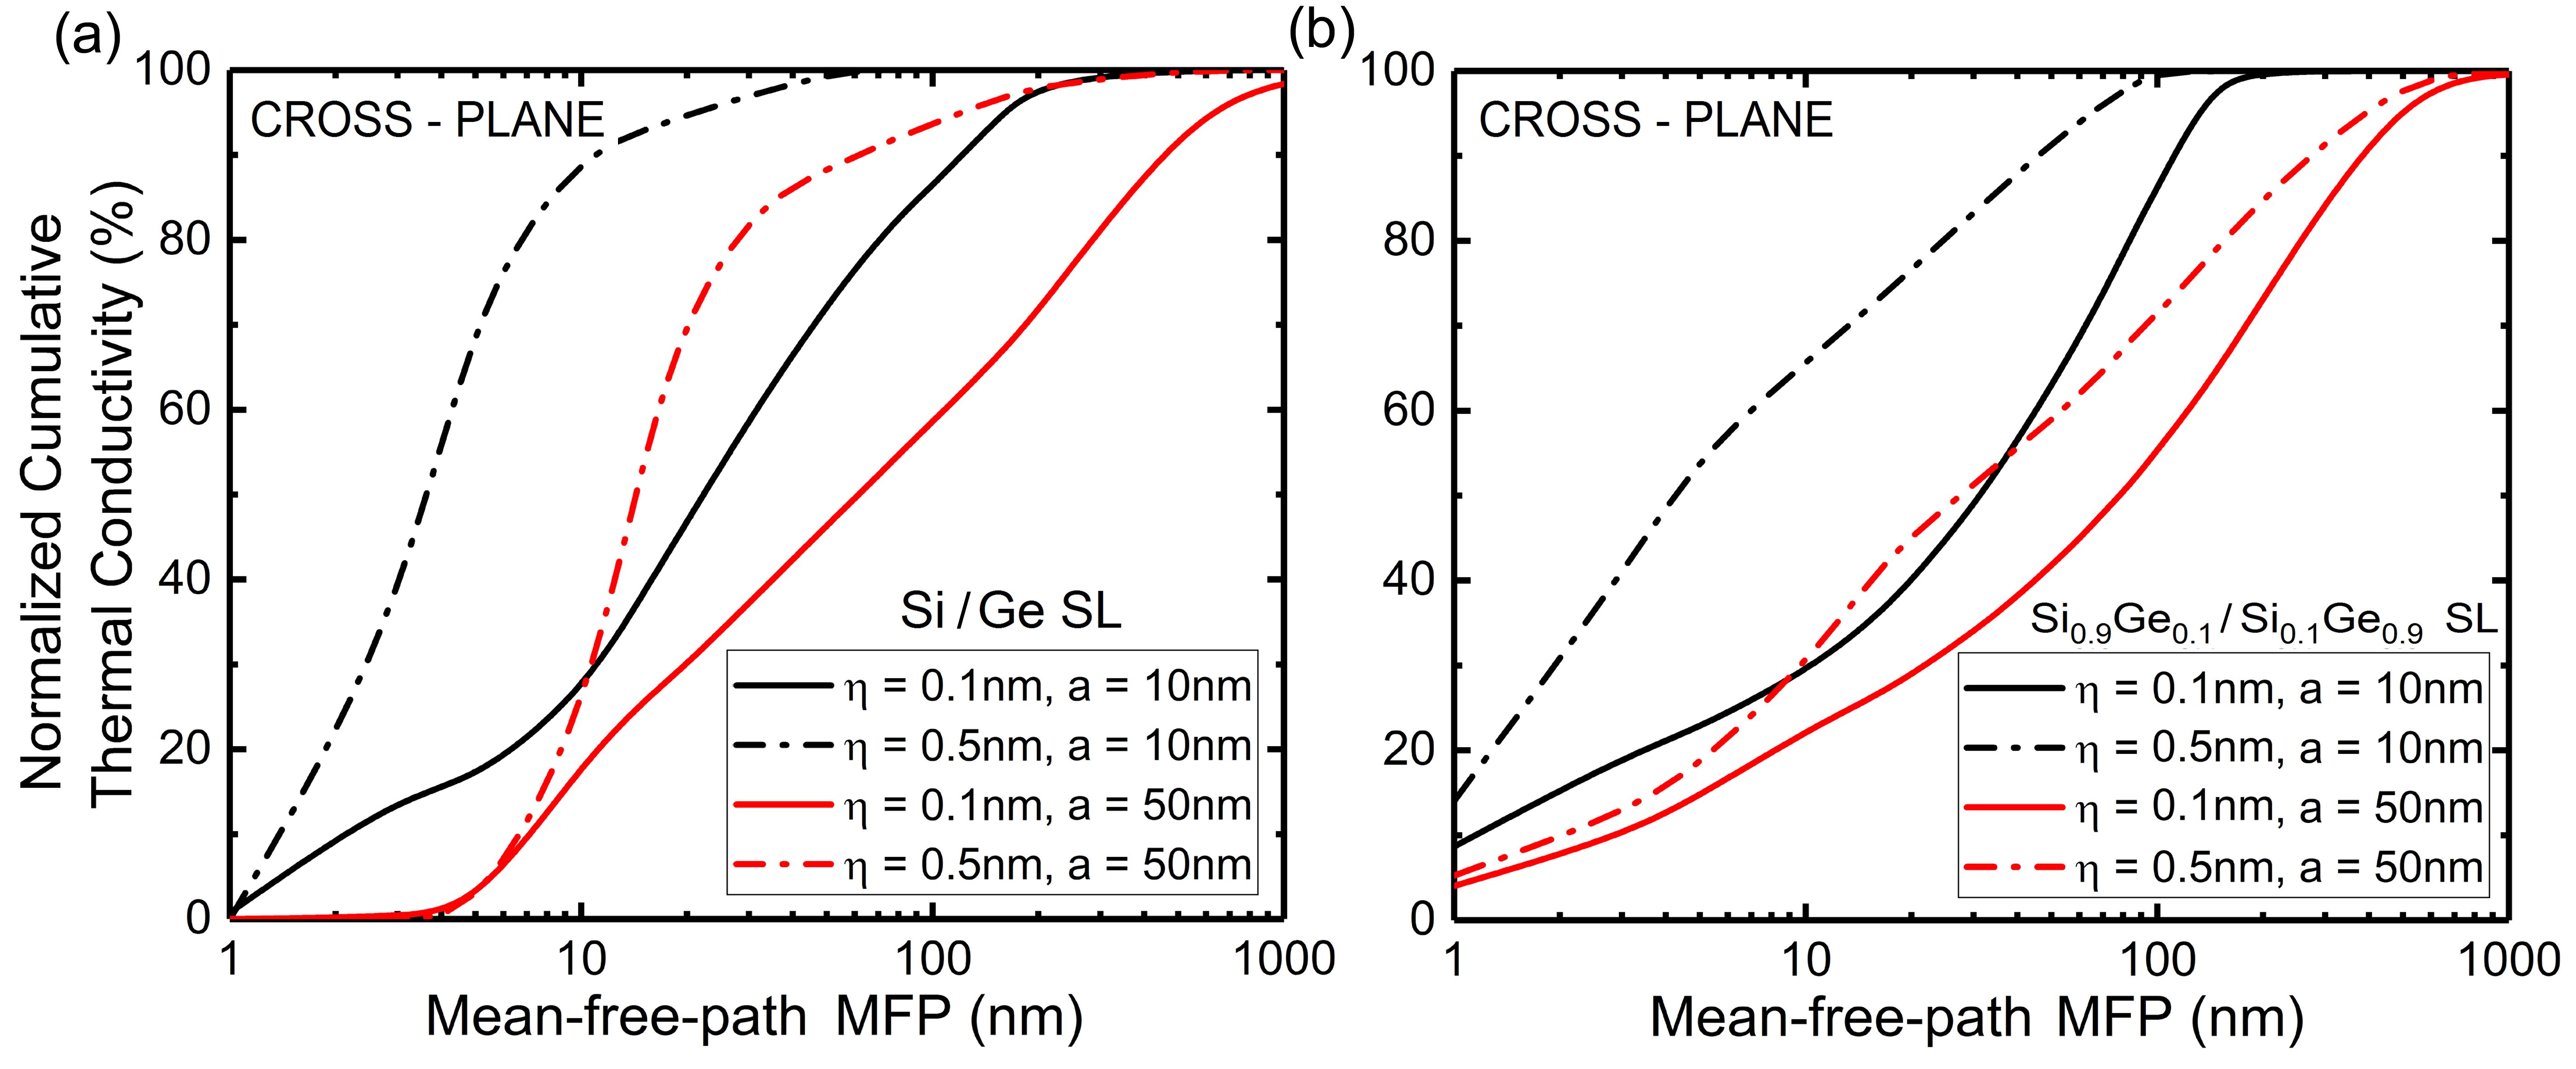
\includegraphics[width=1.0\textwidth]{figures/ch6/Fig9.jpg}
  \caption{Cross-plane thermal conductivity spectra at \gls{T} = 300 K as a function of phonon mean-free-path for superlattices of period 50 nm (red lines) and 10 nm (black lines) for smooth and rough interfaces in (a) Si/Ge and (b) \sige{0.90}{0.10}/\sige{0.10}{0.90} superlattices.}
  \label{fig:ch6-9}
\end{figure}

\section{Summary}
In this chapter, we extended the methodology developed in \Cref{chap:layered} to quantitatively predict and fundamentally understand incoherent cross-plane thermal transport in superlattices. We used our developed approach to study Si/Ge and SiGe alloyed superlattices in order to understand the role of all relevant length scales, i.e., interface roughness, period thickness, total structure thickness, phonon mean-free-path, and wavelength in the underlying thermal transport processes. Additionally, we unveiled the effects of alloying and temperature on cross-plane thermal transport in these superlattices. We found that thermal transport in cross-plane structures can be ballistic across the entire superlattice even at room temperatures. In addition, the contribution of large wavelength phonons is significantly suppressed in contrast to in-plane thermal transport, constraining the wavelength spectrum to less than 10 nm. These findings are essential toward efforts to rationally manipulating phonon transport and for future design of thermal transport processes in superlattices.




%%%%%%%%%%%%%%%%
% Chapter 7
%%%%%%%%%%%%%%%%

%!TEX root = thesis.tex
\chapter{Conclusions}
\label{chap:conc}
\section{Impact of Dissertation}
The work presented in this dissertation comprises of models of thermal conduction in a number of semiconductor nanostructures, beginning with incorporating surface descriptors to create predictive models and bridge the differences between experimental and computational research, to uncovering a novel phonon coupling mechanism to modulate thermal transport in layered nanomaterials. While we primarily utilized silicon and germanium as elements of choice, the general insights about the flow of heat in different nanostructures are applicable across a wide range of semiconductors. 

\par The lack of existing predictive models that could account for all the relevant physical descriptors in the phonon-surface scattering motivated the study in \Cref{chap:predictive}. The objective of creating phonon transport models which rely on experimentally quantifiable surface descriptors (i.e. surface roughness and correlation length) and embody key physics of phonon-transport (i.e. surface scattering dependence on incident phonon momentum, incident angle and do not treat internal and surface scattering as volumetric phenomena) was achieved with the use of Beckmann-Kirchhoff surface scattering theory along with surface shadowing correction. After developing the phonon-surface scattering model, we showed that the model accurately agrees with the experimentally thermal conductivities of nanowires and thin-films. Moving beyond the traditionally measured thermal conductivity, we predicted that a decrease in the nanostructure size and increased roughness and correlation lengths makes the thermal spectra significantly shift towards phonons with short wavelengths and mean-free-paths. The versatility of the predictive model was highlighted by the results of thermal spectra for bulk materials, which showed excellent agreement with recent experimental approaches that reconstruct the mean-free-path heat spectra. Our predictions showed how the specific surface properties and temperatures can significantly modify the thermal conductivity accumulation, thereby opening a way forward to the rational design of the semiconductor-air interfaces, which can be utilized to tailor the desired thermal transport properties in nanostructures. 

\par We extended the phonon-transport model in \Cref{chap:diff_boundary} to move beyond the assumption of symmetric boundaries in thin-films, with the motivation of a better replication of typical experimental nanostructures. The methods developed move beyond the commonly used diffuse scattering surface assumptions, enabling the surfaces of the thin films to be precisely described via their individual specularities. Furthermore, during this development, we highlighted the equivalence of solving the Boltzmann transport equation by explicitly calculating mean-free-paths or by utilizing the boundary conditions to semi-analytically evaluate non-equilibrium phononic populations. The latter approach is utilized in layered materials discussed in \Cref{chap:layered,chap:slxp}. Our primary objective was to analyze the spatial distribution of thermal flux in asymmetric thin-films.We showed that designing the physical properties of thin-film surfaces provides control over the preferential spatial location of thermal flux, which could hold significant potential for rational design of thermal materials. Additionally, we showed the existence of heat transport regimes, controlled by the surface properties resembling fluid flow in confined geometries.
 
\par Our ability to model asymmetric structures proved central in quantitatively predicting thermal transport in nanotubes in \Cref{chap:nt}. Semiconductor nanotubes present an exciting avenue to create very thin one-dimensional nanostructures using currently available growth techniques. Due to their large surface-to-volume ratio, nanotubes allow for an effective control over thermal energy transfer. The ability to treat the two boundaries of the nanotubes as distinct from one another allowed us to discriminate between phonon modes that depended on the properties of both the boundaries (NT-modes) and those that were independent of the inner boundary (NW-modes). The versatility of our model allowed us to analyze the impact of nanotube morphology such as shell thicknesses, outer diameters, and surface properties on thermal transport. We concluded that in general, the thermal conductivity of the nanotube depends on the outer diameter even for the same shell thickness. We showed that the experimentally observed independence between these quantities could be explained by a combination of addition of impurity atoms to the Silicon lattice and surface roughness. We also evaluated the frequency and mean-free-path spectra to elucidate and provide insight on the phonon transport mechanisms in low-dimensional nanotube structures.

\par The phonon-surface scattering in all of the nanostructures discussed serves to reduce thermal transport by shortening phononic mean-free-paths. Motivated by the central question, is it possible to increase phononic-mean-free-paths at the nanoscale, we explored thermal transport in layered nanomaterials in \Cref{chap:layered}. We showed that enhanced thermal conductivities can be achieved in semiconductor nanostructures by rationally engineering phonon spectral coupling between materials. By embedding a germanium film between silicon layers, we showed that its thermal conductivity could potentially be increased by more than 100\% at room temperature in contrast to a free standing thin-film and the injection of phonons from the cladding silicon layers created the observed enhancement in thermal conductivity. While analyzing the underlying phonon-injection mechanism we found that the aforesaid increase comes at the cost of a reduction of thermal conductivity of the silicon layers. Our evaluations of the dependence of thermal conductivity modulations of both silicon and germanium layers on structural parameters showed the critically role of layer spacings and interface properties. Thus, we showed a novel phonon-surface behavior beyond the traditional diffusive scattering of phonons that can be tuned to modulate thermal transport. Next, we extended the tri-layer transport analysis to bi-layer structures to elucidate thermal transport in structures of technological importance, i.e. film-on-substrate (FOS) architectures. We observed an unconventional behavior of thermal conductivity variation with film thickness, an increased thermal conductivity with decreasing thickness in \algas{0.1}{0.9} films over GaAs substrate. In contrast, Ge films over Si substrate showed a decreasing thermal conductivity with decreasing thickness. The difference in behavior arose due to the phonon injection from substrate media which is critically dependent on the interplay of acoustic impedance mismatch, materials thermal transport properties, interfacial characteristics, and thickness of thin film atop the substrate. We also determined that a trade-off between interfacial scattering and available volume fraction for enhancement play a crucial role in determining the thermal conductivity of the FOS. The analysis of the FOS architectures suggests that experimental measurement of thermal conductivity of thin-films needs to account for thermal coupling between thin film and substrate and the consequent conductivity modification and highlights the need to develop rigorous conductivity read-out models for experiments.

\par Lastly, we utilized our models of layered nanomaterials to study cross-plane thermal conduction in silicon-germanium superlattices considering interactions of phonons with multiple structural length scales in \Cref{chap:slxp}. Our results clearly highlighted the need for quantifying the impact of all relevant length variables in superlattices, i.e., the mean-free-path and wavelength of phonons, the periodicity of the structure, total size of the superlattice, and the length scale of interfacial disorder, to fully understand the heat conduction in superlattices. Our predictions showed that thermal conduction can be ballistic traveling across multiple low roughness interfaces of the superlattice even at room temperatures. In contrast to in-plane transport, we found that the strong surface scattering encountered in the cross-plane direction limits the phonon transport to mean-free-paths of less than 1 \si{\micro}m and wavelengths less than 10 nm even in alloyed superlattices of periods up to 50 nm. This strong role of boundaries also manifests itself in the form of thermal conductivity anisotropy in superlattices. We also reported the impact of the number of periods and total structural size on the thermal conductivity which is critical for accurate experimental reporting of thermal conductivities.

\section{Possible Directions for Future Work}
There are several interesting research projects that are natural extensions of the work presented in this thesis:

\subsection{Exploring the Limits of Phonon Injection Mechanism}
The complex nature of phonon injection mechanism manifests itself in unique and novel changes to thermal conductivities as highlighted in this thesis. Both the structural properties which include layer thicknesses and surfaces roughness, and the the material properties which involve the dispersion relations and relaxation times, are important to this mechanism.  Further study can help elucidate this mechanism to understand the limits of phonon coupling. For instance, transmission of phonons across interfaces requires propagating modes in both materials. From this perspective, materials with similar phononic dispersions would create a greater degree of phonon spectral coupling. Additionally, we showed that small surface roughness and consequential lower diffusive scattering of phonons increase the spectral coupling between the two materials. Thus, materials with similar lattice constants would favor effective phonon spectral coupling by providing smoother interfaces. Also, the difference in thermal transport properties gives rise to the concept of net phonon injector and acceptor roles for materials. Hence, the search for a system to observe maximized thermal conductivity enhancement and reduction effects would need to account for both the degree of phonon coupling and the difference in thermal properties. For instance, coupling a given material with an extremely high thermal conductivity material such as diamond or graphene could exhibit unique thermal conductivity modulations.  

\subsection{Guided Experiments for Validating Thermal Conductivity Enhancement Predictions}
In order to experimentally validate the predictions of thermal conductivity enhancement presented in this thesis, collaborative effort to fabricate samples with controlled surface disorder and measure layer-by-layer thermal conductivity would be required. In this regard, thermal conductivity measurements on thin-film grown on substrates may provide a better platform since they are better studied and thermoreflectance measurement techniques can be used to validate the findings. Considerations on the ability to fabricate specified layer thicknesses while preserving control over surface properties would need to be kept in mind and typical read-out models from experiments that ignore phonon coupling may need to be improved in order to quantitatively validate the predictions. Concurrently, a sequence of samples with different layer spacings may be utilized to qualitatively validate the predictions presented in this thesis.

\subsection{Coherent Phonons and their Impact on Thermal Transport}
The modulations of thermal transport in this thesis have stemmed from changes in transport properties of phonons that are uncorrelated with their phase, i.e. by considering the particle like behavior of phonons in the form of their mean-free-paths. However, under certain conditions, it is possible for phonons to exhibit coherent interference phenomenon which can manipulate their heat carrying ability by changing the phonon dispersion relations, thereby altering the phonon group velocities and density of states \cite{RN132,RN362}. We estimated the potential impact of such coherent behavior in the form of quantum confinement in thin-films by extracting information from thermal spectra in this thesis. However, in order to provide rigorous calculations further research is needed to account for these changes within a thermal transport model. In particular, the cross-plane transport in superlattices has been shown to be influenced by coherent interference of phonons \cite{RN393}. The presence of smooth surfaces that avoids diffuse scattering favors such coherent interference of phonons \cite{RN132,RN362} allowing the phonons to traverse multiple interfaces. Furthermore, thermal spectra can be tuned so that phonons with lower frequencies and longer mean-free-paths dominate thermal transport, allowing for coherent effects to be strongly expressed. Coherent modifications to phonon transport coupled with the transport models developed in this thesis would encompass the possible scope of modulating thermal transport via nanostructuring in semiconductors.
\todo{Discuss with MM, if need more, possibly combining conduction, convection and radiation effects?}
\par These are just a few of the possibilities that could present exciting avenues for research. As the understanding of phonon transport and the ability to engineer novel nanostructures continues to evolve, it is our hope that this thesis will provide a firm foundation for future exploration of engineering the flow of heat at the nanoscale.

%%Eqn.
%\begin{equation}
%  \sum_{i=1}^{n}{(X_i - \overline{X})^2}^{n}{(X_i - \overline{X})^2}\ . 
%\end{equation}
%
%
% This is a figure
%\begin{figure}
%	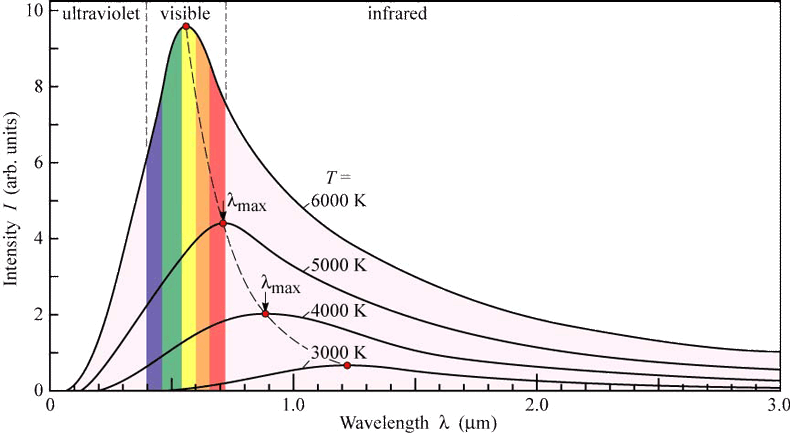
\includegraphics[width=\textwidth]{exampleFigure.png}
%	\caption{This is an example Figure.}
%	\label{Figure in Chapter 6}
%\end{figure}
%
%\begin{equation}\label{key}
%\sqrt{\cos(x)}=1
%\end{equation}
%This implies that,
%\begin{equation}\label{eq:test}
%\boxed{\text{Free particle is: } K_{k+1}=P_ka_{k+1}^T\left(a_{k+1}P_ka_{k+1}^T+I_N\right)^{-1}}
%\end{equation}
%
%\begin{equation}\label{eq:test2}
%\boxed{\text{Free particle is: }\  \Psi(\mathbf{x},t)=e^{i(\mathbf{k}.\mathbf{x}-\omega t)}}
%\end{equation}
%
%\begin{equation} \label{tranfdc}
%\begin{split}
%T_v(s) & = \frac{V_{dc}(s)}{V_{dcref}(s)}
%= \frac{\omega _B}{B}
%\frac{k_{pdc}s + k_{idc}} {s^2 + \frac{ k_{pdc} \omega _B s} {B} +
%	\frac{k_{idc} \omega _B} {B}} ,  \\
%%
%T_i(s) & = \frac{V_{dc}(s)}{i_{l}(s)}
%= - \frac{\omega _B}{B} \frac{s} {s^2
%	+ \frac{ k_{pdc} \omega _B s} {B} + \frac{k_{idc} \omega _B} {B}} .
%\end{split}
%\end{equation}
%
%
%\begin{align*}
%x&=y           &  w &=z              &  a&=b+c\\
%2x&=-y         &  3w&=\frac{1}{2}z   &  a&=b\\
%-4 + 5x&=2+y   &  w+2&=-1+w          &  ab&=cb
%\end{align*}



%%%%%%%%%%%%%%%%
% Appendices
%%%%%%%%%%%%%%%%

\begin{appendices}
\crefalias{chapter}{appendix}
%Some Table of Contents entry formatting
\addtocontents{toc}{\protect\renewcommand{\protect\cftchappresnum}{\appendixname\space}}
\addtocontents{toc}{\protect\renewcommand{\protect\cftchapnumwidth}{6em}}

%Begin individual appendices, separated as chapters
\chapter{Comparison of Acoustic Phonon Relaxation Rates in Silicon}
\label{app:si_relaxation_rates}
The accurate establishment of the bulk phonon relaxation times is an active research area involving experimental techniques and theoretical models ranging from first-principle to phenomenological approaches \cite{stokes_bulkSi_tau,RN273,RN217,ownNW,RN236}. Although initial theory assumed bulk relaxation times to be constant (i.e. frequency independent) the necessity for frequency-dependent times was realized and incorporated in the theoretical models. In recent years, first-principle approaches based on density-functional-theory (DFT) have provided theoretical predictions for the frequency-dependence of the bulk phonon relaxation times in a variety of materials including Silicon \cite{stokes_bulkSi_tau}. In this thesis, we use expressions obtained by assuming a $\omega^{-2}$ and  $\omega^{-4}$ dependence of relaxation times by Umklapp scattering and isotope scattering effects, respectively \cite{maldovan2011tf}. Optical modes are neglected, as owing to their low group velocities their contribution to thermal conductivity is low \cite{RN212}. 

The phonon relaxation times for bulk silicon at room temperature from various approaches are plotted in \Cref{fig:appendix-LA,fig:appendix-TA}. Overall, the different approaches yield the same range of relaxation times. The results show that models obtained by different approaches vary at very low frequencies, however it is important to note that low frequency phonons are non-dominant heat carriers in Si at room temperatures. The close agreement between the results from the approach used in this thesis (taken from Ref. \cite{maldovan2011tf}) and DFT calculations \cite{stokes_bulkSi_tau,RN244} especially for the transverse branch (dominant for heat transport) is noteworthy.

\begin{figure}[hbt]
	\centering 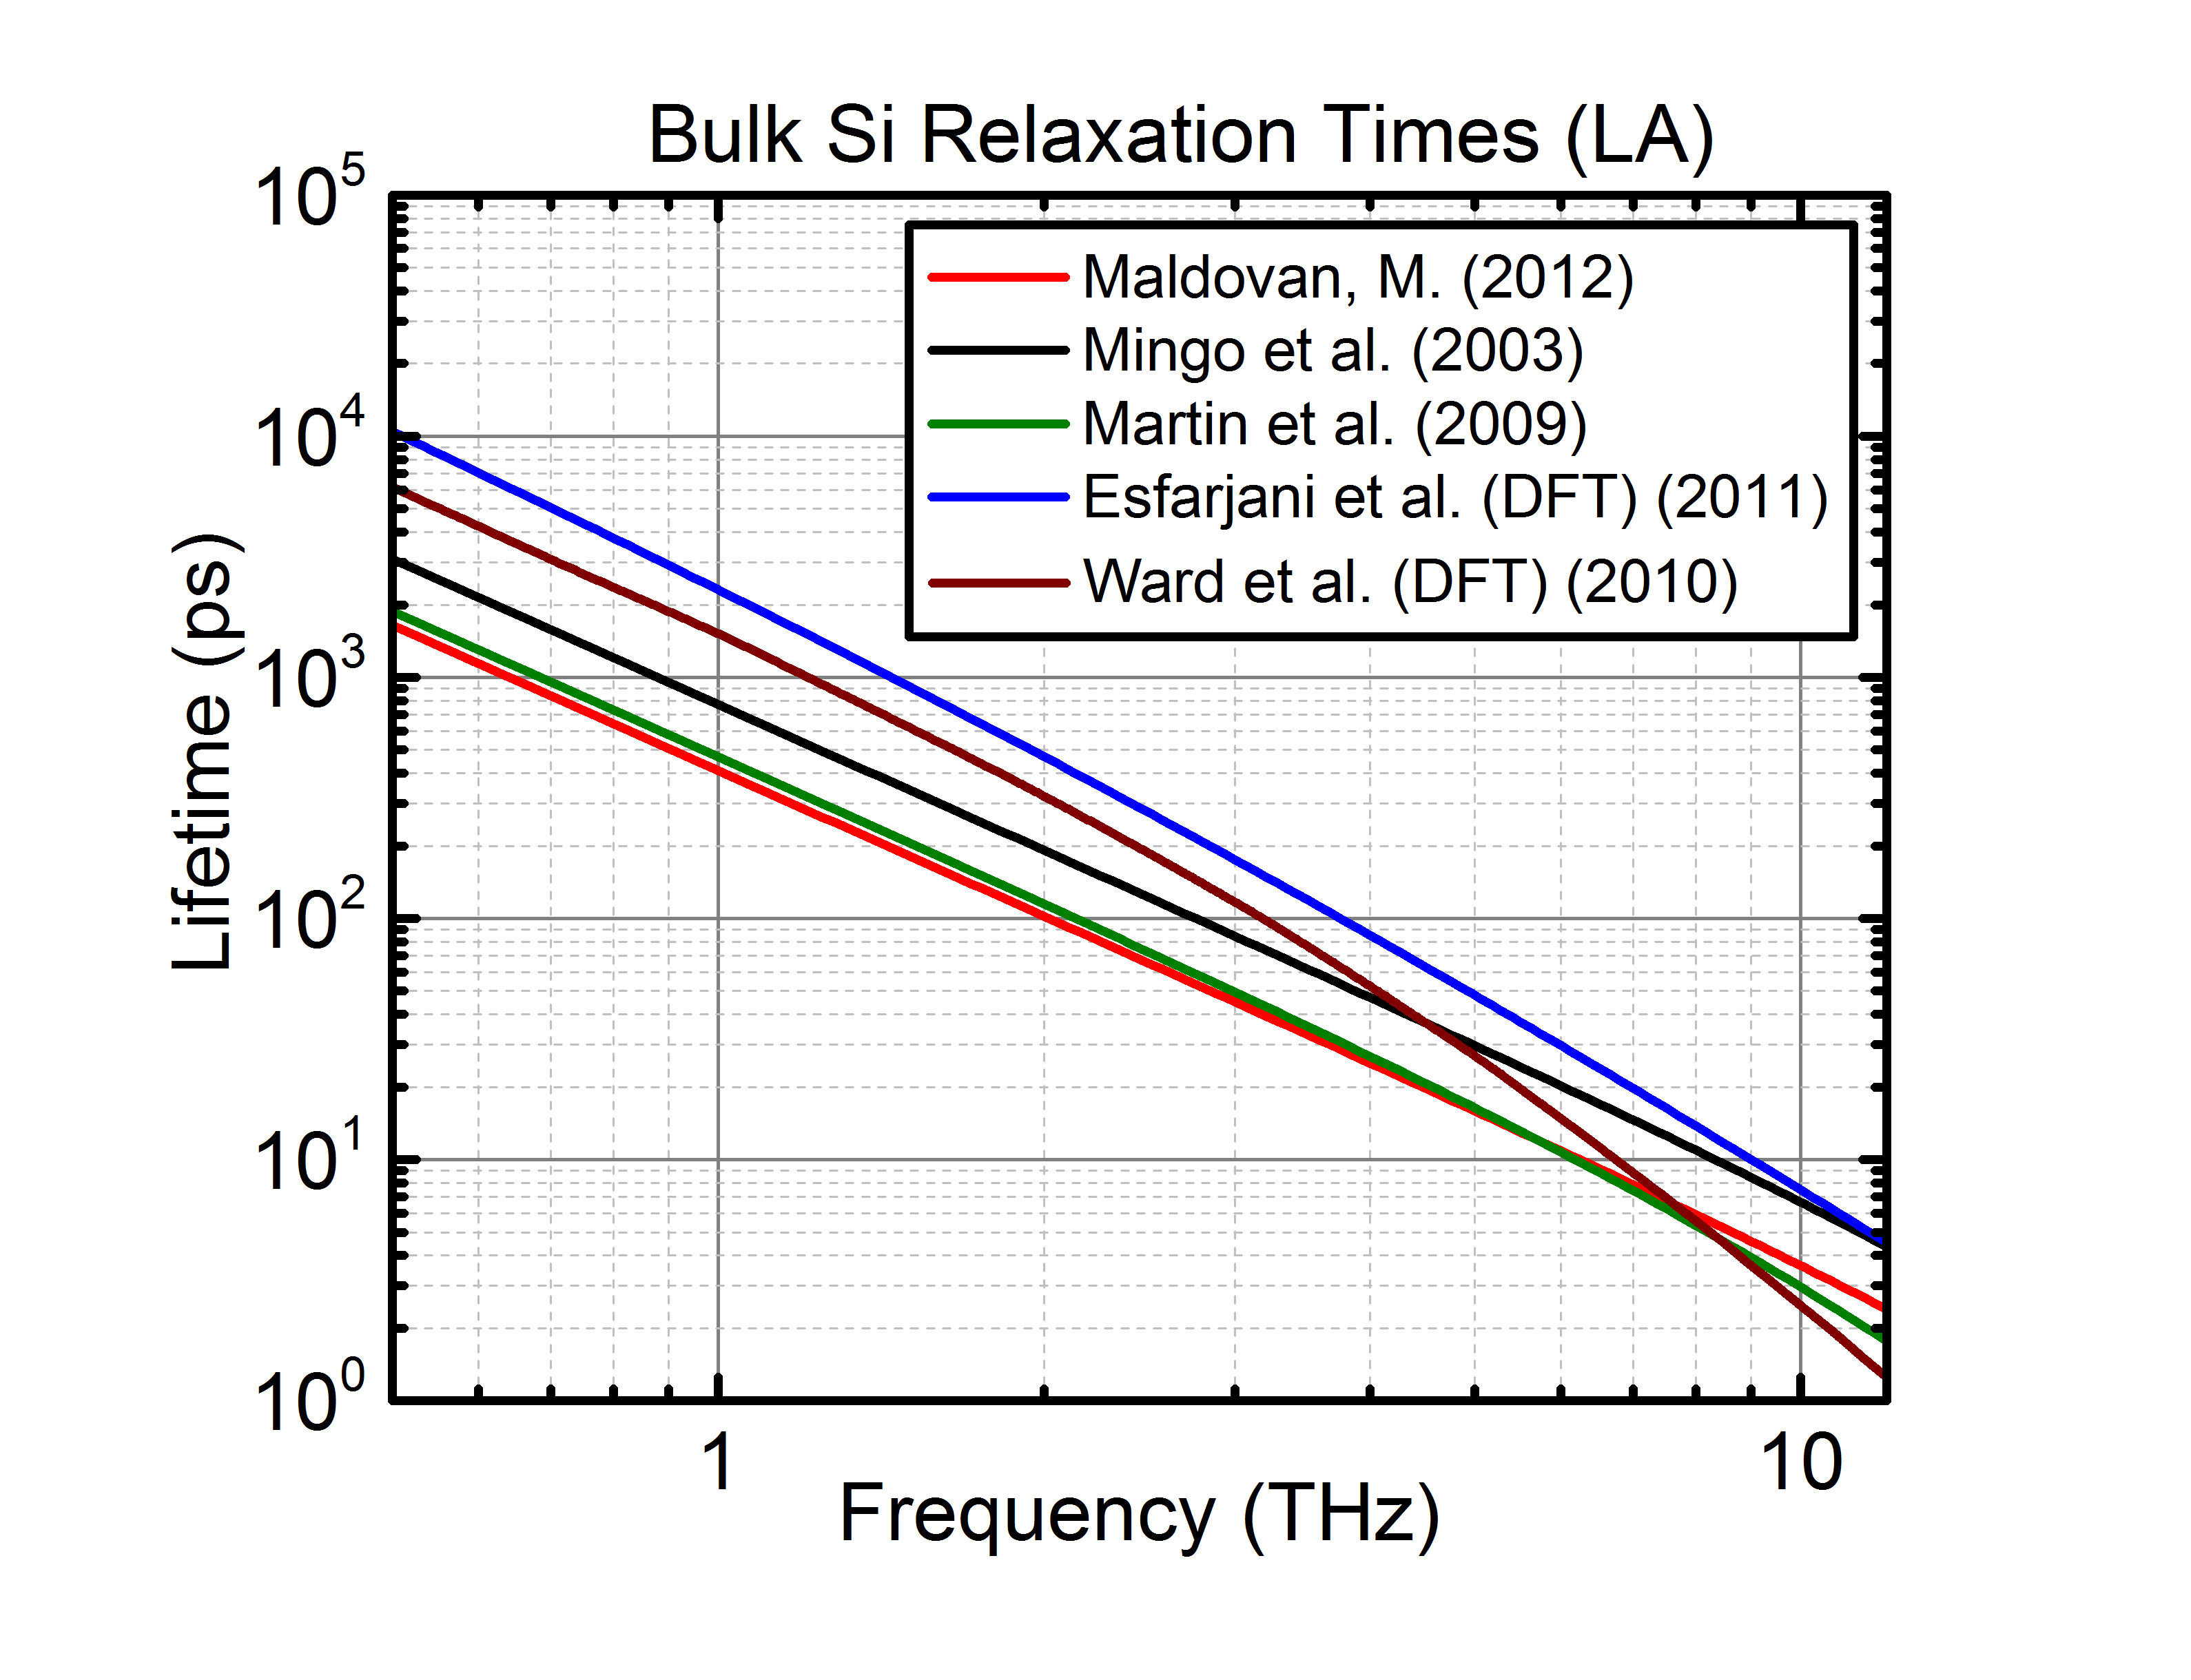
\includegraphics[width=0.80\textwidth]{/ch99/FigureA1.jpg}
	\caption{Relaxation times for longitudinal acoustic (LA) phonons in bulk Silicon at 300 K.}
	\label{fig:appendix-LA}
\end{figure}

\begin{figure}[hbt]
	\centering 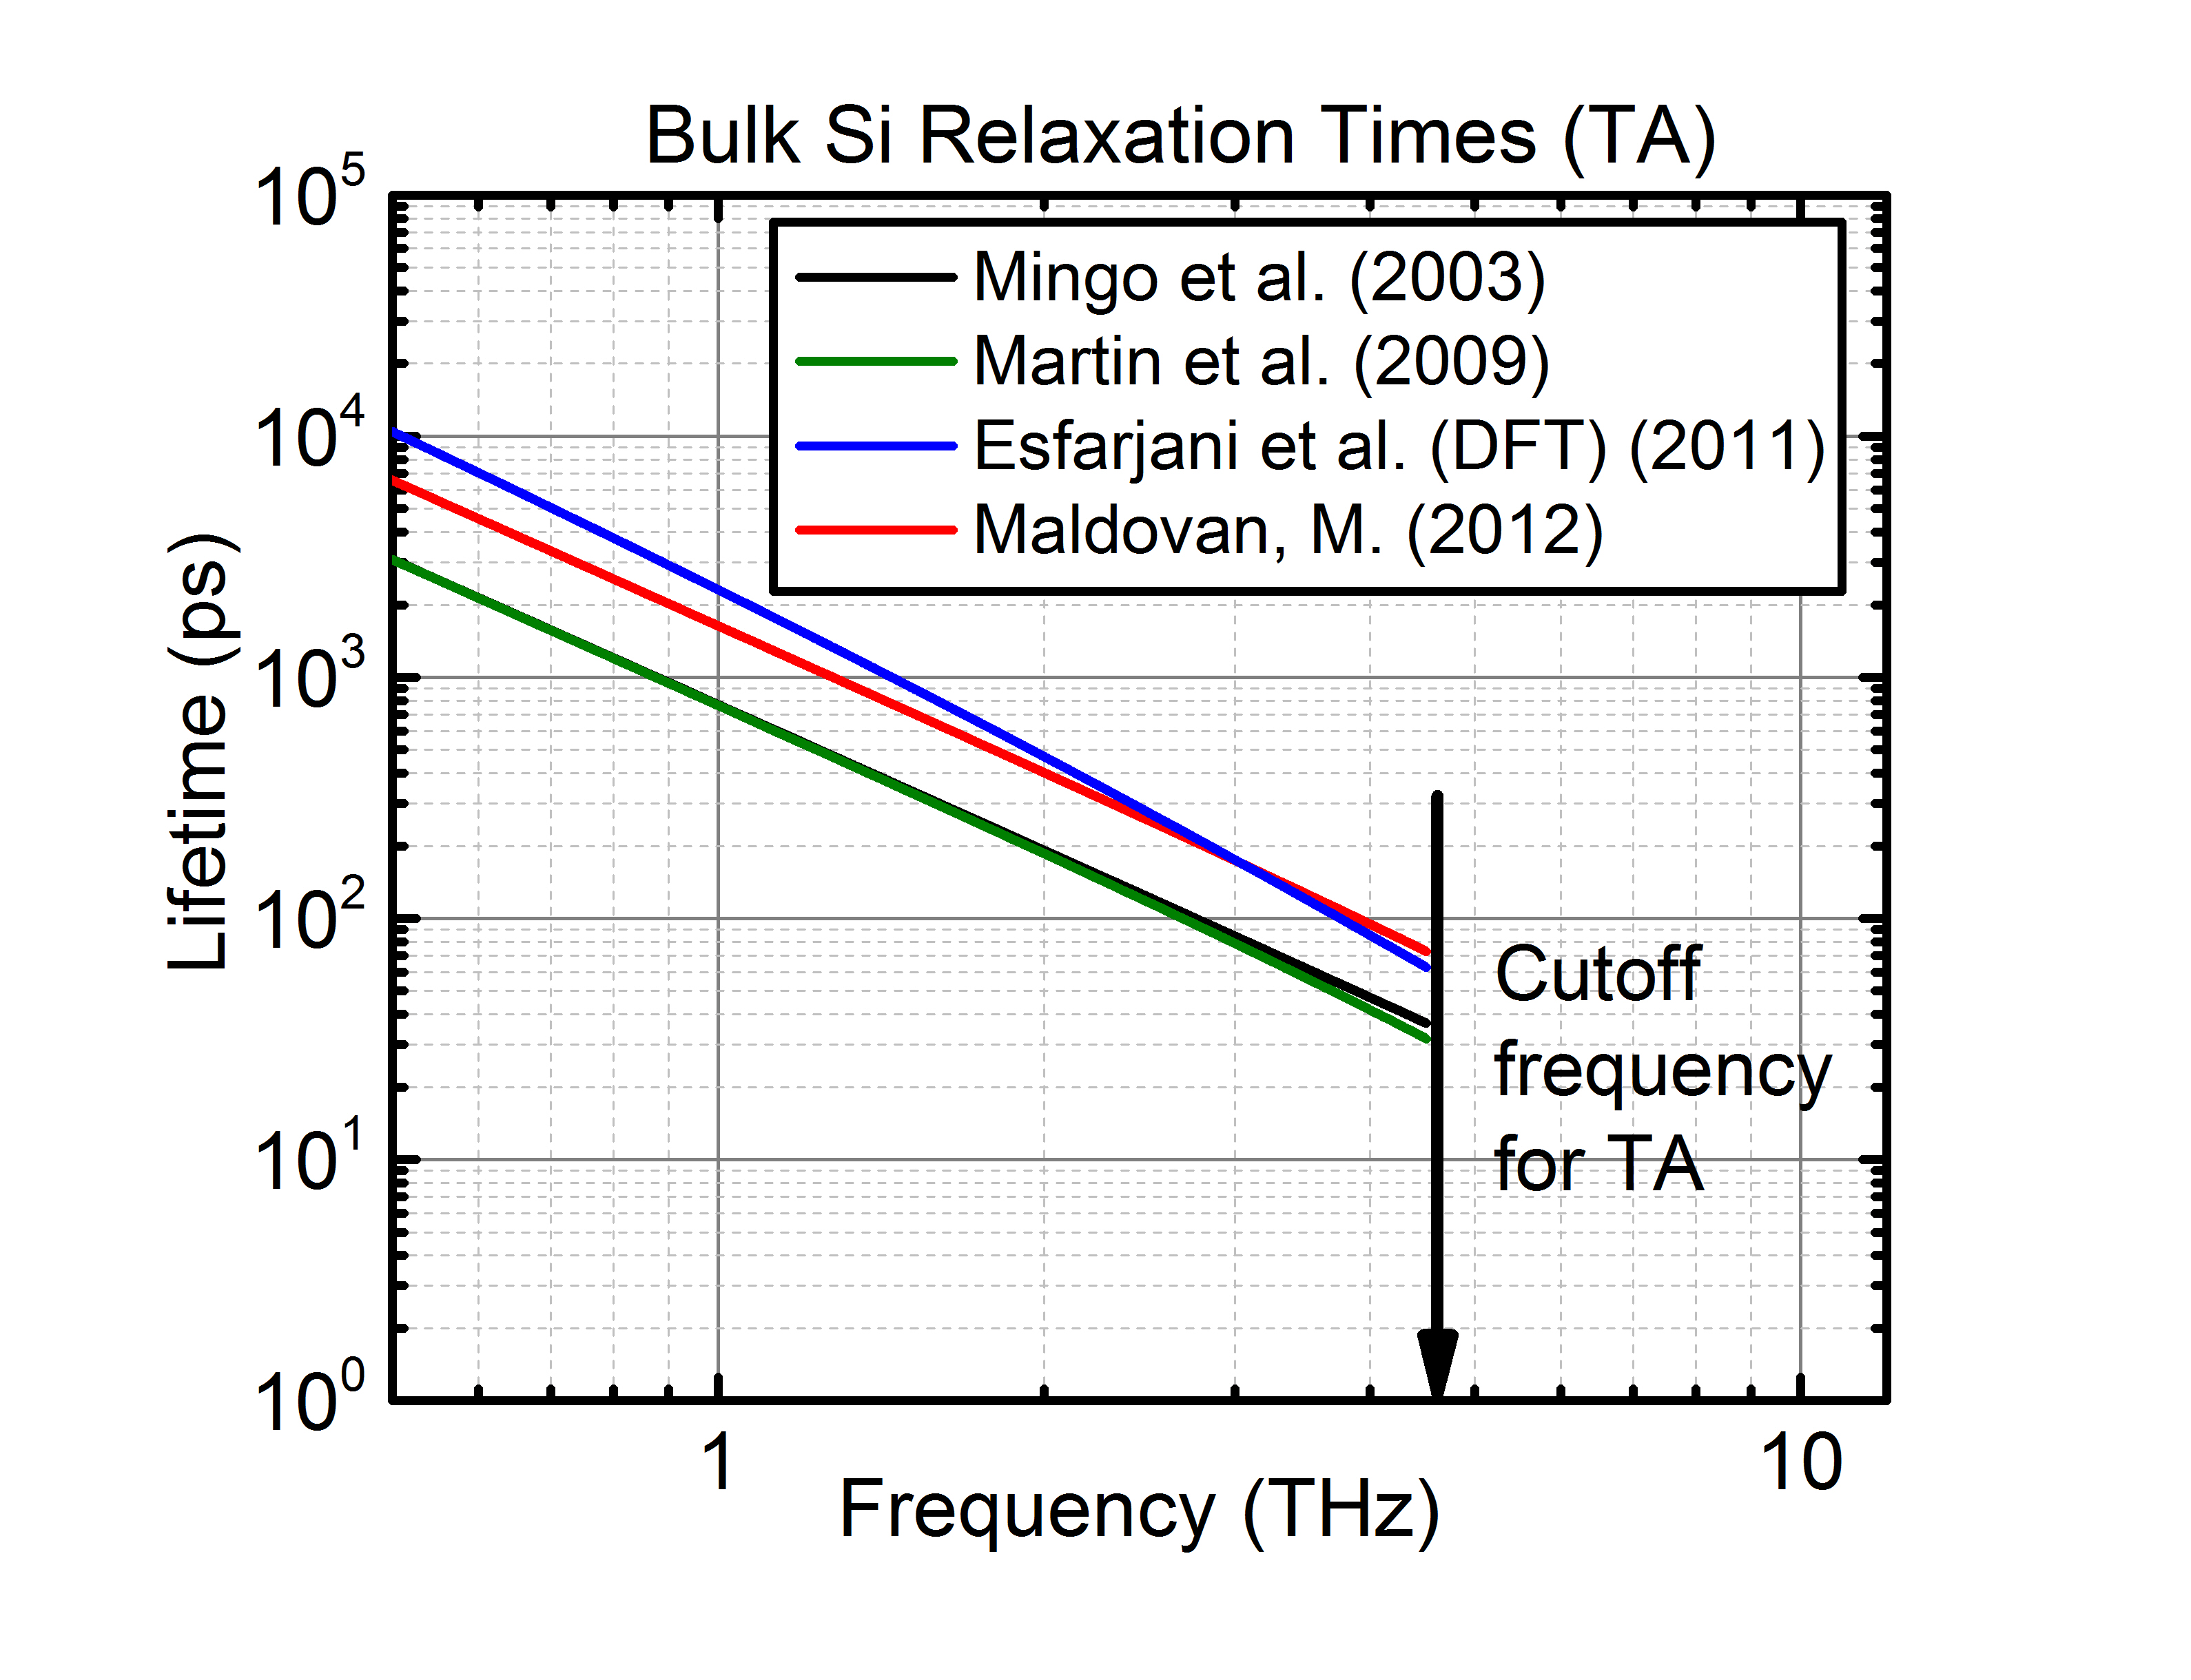
\includegraphics[width=0.80\textwidth]{/ch99/FigureA2.jpg}
	\caption{Relaxation times for transverse acoustic (TA) phonons in bulk Silicon at 300 K.}
	\label{fig:appendix-TA}
\end{figure}

%-------
\chapter{Numerical Calculations of Shadowing Function}
\label{app:shadowing}
A numerical calculation of shadowing function $S(\theta,\varphi)$ i.e. \Cref{eq:shadowing-full} is shown in \Cref{fig:appendix-Shadowing}. The plots are presented for two different cases: \gls{cl} = 5\gls{eta} (filled symbol) and \gls{cl} = 10\gls{eta} (open symbol). For smaller correlation lengths, the shadowing function approaches a lower value compared to a larger correlation length. This is intuitive and follows the previous discussion that a higher correlation length indicates a more continuous surface with lower number of sharp peaks and valleys, thus, reducing the number of points being shadowed. For incident angles close to the normal, a higher value of shadowing function is achieved, which is reasonable as the ability of a point to shadow a surface is negligible for small angles of incidence. It can also be seen in the case of higher correlation length, the value of shadowing quickly approaches unity for all incident angles less than \ang{70}. Note that the shadowing function used for calculations in our heat transport model is a subset of the general function presented. The locus generated by joining the points lying on the curves for which incident angles and observation angles are taken to be equal would provide the required shadowing function for the specular direction $S(\theta,\varphi=\theta)$.
\begin{figure}[hbt]
	\centering 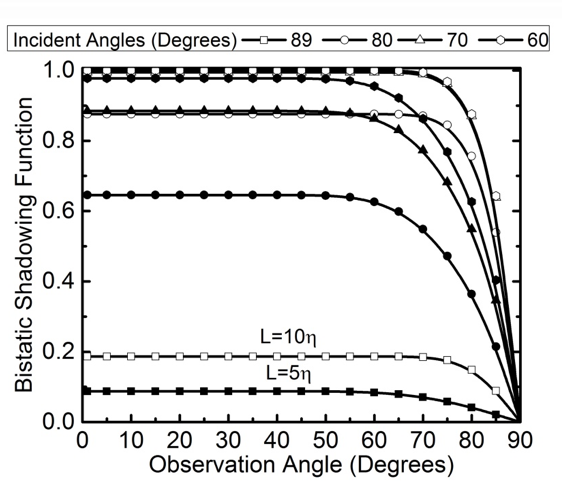
\includegraphics[width=0.85\textwidth]{/ch99/FigureB1.png}
	\caption{Bistatic shadowing function calculated for four representative incident angles and observation angles between 0 and $\pi$/2 radians. Open and filled symbols represent a surface correlation length \gls{cl} = 10\gls{eta} and \gls{cl} = 5\gls{eta}, respectively.}
	\label{fig:appendix-Shadowing}
\end{figure}
\end{appendices}

%%%%%%%%%%%%%%%%
% References
%%%%%%%%%%%%%%%%

\begin{singlespace}  % use single-line spacing for multi-line text within a single reference
	\setlength\bibitemsep{\baselineskip}  %manually set separataion betwen items in bibliography to double space
	\printbibliography[title={References}]
\end{singlespace}
	
\addcontentsline{toc}{chapter}{References}  %add References section to Table of Contents

%%%%%%%%%%%%%%%%
% Vita
% Only for PhD students
% Masters students remove this line
%%%%%%%%%%%%%%%%
%\chapter*{Vita}
\addcontentsline{toc}{chapter}{Vita}  %add Vita section to Table of Contents
\textbf{Abhinav Malhotra} was born in Amritsar, India in 1990. He is a Professor in Fine Arts at the University of Barcelona and member of the Faculty of Fine Arts PhD programme. He has held individual exhibitions of his sculptures and drawings in Barcelona, Madrid, Gerona, The Hague, Amsterdam and Brussels. He currently works on public art projects for several architects in Barcelona. His sculptures have been acquired by public and private collections in Europe, South Korea and the USA.



\end{document}
